\documentclass[12pt]{book}

\usepackage{booktabs}
\usepackage{csquotes}
\usepackage{enumitem}
\usepackage{verbatim}  % Needed for the "comment" environment to make LaTeX comments

\usepackage{longtable}

\usepackage{pdfpages}
\usepackage{listings}


%%% Llamadas de rmarkdown
\usepackage{lmodern}
\usepackage{amssymb,amsmath}
\usepackage{ifxetex,ifluatex}
\usepackage{fixltx2e} % provides \textsubscript
\ifnum 0\ifxetex 1\fi\ifluatex 1\fi=0 % if pdftex
  \usepackage[T1]{fontenc}
  \usepackage[utf8]{inputenc}
\else % if luatex or xelatex
  \ifxetex
    \usepackage{mathspec}
  \else
    \usepackage{fontspec}
  \fi
  \defaultfontfeatures{Ligatures=TeX,Scale=MatchLowercase}
\fi
% use upquote if available, for straight quotes in verbatim environments
\IfFileExists{upquote.sty}{\usepackage{upquote}}{}
% use microtype if available
\IfFileExists{microtype.sty}{%
\usepackage{microtype}
\UseMicrotypeSet[protrusion]{basicmath} % disable protrusion for tt fonts
}{}
\usepackage[margin=1in]{geometry}
\usepackage{hyperref}
\hypersetup{unicode=true,
            pdftitle={aprendeR},
            pdfborder={0 0 0},
            breaklinks=true}
\urlstyle{same}  % don't use monospace font for urls
\usepackage{color}
\usepackage{fancyvrb}
\newcommand{\VerbBar}{|}
\newcommand{\VERB}{\Verb[commandchars=\\\{\}]}
\DefineVerbatimEnvironment{Highlighting}{Verbatim}{commandchars=\\\{\}}
% Add ',fontsize=\small' for more characters per line
\usepackage{framed}
\definecolor{shadecolor}{RGB}{248,248,248}
\newenvironment{Shaded}{\begin{snugshade}}{\end{snugshade}}
\newcommand{\KeywordTok}[1]{\textcolor[rgb]{0.13,0.29,0.53}{\textbf{#1}}}
\newcommand{\DataTypeTok}[1]{\textcolor[rgb]{0.13,0.29,0.53}{#1}}
\newcommand{\DecValTok}[1]{\textcolor[rgb]{0.00,0.00,0.81}{#1}}
\newcommand{\BaseNTok}[1]{\textcolor[rgb]{0.00,0.00,0.81}{#1}}
\newcommand{\FloatTok}[1]{\textcolor[rgb]{0.00,0.00,0.81}{#1}}
\newcommand{\ConstantTok}[1]{\textcolor[rgb]{0.00,0.00,0.00}{#1}}
\newcommand{\CharTok}[1]{\textcolor[rgb]{0.31,0.60,0.02}{#1}}
\newcommand{\SpecialCharTok}[1]{\textcolor[rgb]{0.00,0.00,0.00}{#1}}
\newcommand{\StringTok}[1]{\textcolor[rgb]{0.31,0.60,0.02}{#1}}
\newcommand{\VerbatimStringTok}[1]{\textcolor[rgb]{0.31,0.60,0.02}{#1}}
\newcommand{\SpecialStringTok}[1]{\textcolor[rgb]{0.31,0.60,0.02}{#1}}
\newcommand{\ImportTok}[1]{#1}
\newcommand{\CommentTok}[1]{\textcolor[rgb]{0.56,0.35,0.01}{\textit{#1}}}
\newcommand{\DocumentationTok}[1]{\textcolor[rgb]{0.56,0.35,0.01}{\textbf{\textit{#1}}}}
\newcommand{\AnnotationTok}[1]{\textcolor[rgb]{0.56,0.35,0.01}{\textbf{\textit{#1}}}}
\newcommand{\CommentVarTok}[1]{\textcolor[rgb]{0.56,0.35,0.01}{\textbf{\textit{#1}}}}
\newcommand{\OtherTok}[1]{\textcolor[rgb]{0.56,0.35,0.01}{#1}}
\newcommand{\FunctionTok}[1]{\textcolor[rgb]{0.00,0.00,0.00}{#1}}
\newcommand{\VariableTok}[1]{\textcolor[rgb]{0.00,0.00,0.00}{#1}}
\newcommand{\ControlFlowTok}[1]{\textcolor[rgb]{0.13,0.29,0.53}{\textbf{#1}}}
\newcommand{\OperatorTok}[1]{\textcolor[rgb]{0.81,0.36,0.00}{\textbf{#1}}}
\newcommand{\BuiltInTok}[1]{#1}
\newcommand{\ExtensionTok}[1]{#1}
\newcommand{\PreprocessorTok}[1]{\textcolor[rgb]{0.56,0.35,0.01}{\textit{#1}}}
\newcommand{\AttributeTok}[1]{\textcolor[rgb]{0.77,0.63,0.00}{#1}}
\newcommand{\RegionMarkerTok}[1]{#1}
\newcommand{\InformationTok}[1]{\textcolor[rgb]{0.56,0.35,0.01}{\textbf{\textit{#1}}}}
\newcommand{\WarningTok}[1]{\textcolor[rgb]{0.56,0.35,0.01}{\textbf{\textit{#1}}}}
\newcommand{\AlertTok}[1]{\textcolor[rgb]{0.94,0.16,0.16}{#1}}
\newcommand{\ErrorTok}[1]{\textcolor[rgb]{0.64,0.00,0.00}{\textbf{#1}}}
\newcommand{\NormalTok}[1]{#1}
\usepackage{graphicx,grffile}
\makeatletter
\def\maxwidth{\ifdim\Gin@nat@width>\linewidth\linewidth\else\Gin@nat@width\fi}
\def\maxheight{\ifdim\Gin@nat@height>\textheight\textheight\else\Gin@nat@height\fi}
\makeatother
% Scale images if necessary, so that they will not overflow the page
% margins by default, and it is still possible to overwrite the defaults
% using explicit options in \includegraphics[width, height, ...]{}
\setkeys{Gin}{width=\maxwidth,height=\maxheight,keepaspectratio}
\IfFileExists{parskip.sty}{%
\usepackage{parskip}
}{% else
\setlength{\parindent}{0pt}
\setlength{\parskip}{6pt plus 2pt minus 1pt}
}
\setlength{\emergencystretch}{3em}  % prevent overfull lines
\providecommand{\tightlist}{%
  \setlength{\itemsep}{0pt}\setlength{\parskip}{0pt}}
\setcounter{secnumdepth}{0}
% Redefines (sub)paragraphs to behave more like sections
\ifx\paragraph\undefined\else
\let\oldparagraph\paragraph
\renewcommand{\paragraph}[1]{\oldparagraph{#1}\mbox{}}
\fi
\ifx\subparagraph\undefined\else
\let\oldsubparagraph\subparagraph
\renewcommand{\subparagraph}[1]{\oldsubparagraph{#1}\mbox{}}
\fi

%%% Use protect on footnotes to avoid problems with footnotes in titles
\let\rmarkdownfootnote\footnote%
\def\footnote{\protect\rmarkdownfootnote}

%%% Change title format to be more compact
\usepackage{titling}

% Create subtitle command for use in maketitle
\newcommand{\subtitle}[1]{
  \posttitle{
    \begin{center}\large#1\end{center}
    }
}

\setlength{\droptitle}{-2em}
  \title{aprendeR}
  \pretitle{\vspace{\droptitle}\centering\huge}
  \posttitle{\par}
  \author{}
  \preauthor{}\postauthor{}
  \date{}
  \predate{}\postdate{}

\usepackage[
  backend=biber,
  style=alphabetic,
  sorting=ynt,
  citestyle=authoryear
  ]{biblatex}
\addbibresource{lit/bib.bib}

\usepackage[utf8]{inputenc}
\usepackage[spanish]{babel}

%%%% Frames
\ifxetex
    \makeatletter % undo the wrong changes made by mathspec
    \let\RequirePackage\original@RequirePackage
    \let\usepackage\RequirePackage
    \makeatother
\fi

\usepackage{xcolor}
\usepackage[tikz]{bclogo}
\usepackage[framemethod=tikz]{mdframed}
\usepackage{lipsum}
\usepackage[many]{tcolorbox}

\definecolor{bgblue}{RGB}{245,243,253}
\definecolor{ttblue}{RGB}{91,194,224}
\definecolor{llred}{RGB}{255,228,225}
\definecolor{bbblack}{RGB}{0,0,0}

\mdfdefinestyle{mystyle}{%
  rightline=true,
  innerleftmargin=10,
  innerrightmargin=10,
  outerlinewidth=3pt,
  topline=false,
  rightline=true,
  bottomline=false,
  skipabove=\topsep,
  skipbelow=\topsep
}

\newtcolorbox{curiosidad}[1][]{
  breakable,
  title=#1,
  colback=white,
  colbacktitle=white,
  coltitle=black,
  fonttitle=\bfseries,
  bottomrule=0pt,
  toprule=0pt,
  leftrule=3pt,
  rightrule=3pt,
  titlerule=0pt,
  arc=0pt,
  outer arc=0pt,
  colframe=black,
}

\newtcolorbox{nota}[1][]{
  breakable,
  freelance,
  title=#1,
  colback=white,
  colbacktitle=white,
  coltitle=black,
  fonttitle=\bfseries,
  bottomrule=0pt,
  boxrule=0pt,
  colframe=white,
  overlay unbroken and first={
  \draw[red!75!black,line width=3pt]
    ([xshift=5pt]frame.north west) -- 
    (frame.north west) -- 
    (frame.south west);
  \draw[red!75!black,line width=3pt]
    ([xshift=-5pt]frame.north east) -- 
    (frame.north east) -- 
    (frame.south east);
  },
  overlay unbroken app={
  \draw[red!75!black,line width=3pt,line cap=rect]
    (frame.south west) -- 
    ([xshift=5pt]frame.south west);
  \draw[red!75!black,line width=3pt,line cap=rect]
    (frame.south east) -- 
    ([xshift=-5pt]frame.south east);
  },
  overlay middle and last={
  \draw[red!75!black,line width=3pt]
    (frame.north west) -- 
    (frame.south west);
  \draw[red!75!black,line width=3pt]
    (frame.north east) -- 
    (frame.south east);
  },
  overlay last app={
  \draw[red!75!black,line width=3pt,line cap=rect]
    (frame.south west) --
    ([xshift=5pt]frame.south west);
  \draw[red!75!black,line width=3pt,line cap=rect]
    (frame.south east) --
    ([xshift=-5pt]frame.south east);
  },
}

%%%
\usepackage{standalone}
\usepackage{float}

\usepackage[normalem]{ulem}
% avoid problems with \sout in headers with hyperref:
\pdfstringdefDisableCommands{\renewcommand{\sout}{}}

\providecommand{\tightlist}{%
  \setlength{\itemsep}{0pt}\setlength{\parskip}{0pt}}
%% USA 12.5 CENTIMETROS PARA EL MARGEN!
%% ----------------------------------------------------------------
\begin{document}
\frontmatter      % Begin Roman style (i, ii, iii, iv...) page numbering

% Set up the Title Page
%\title  {Title}

% % title page commented for now
% \maketitle
%% ----------------------------------------------------------------
\tableofcontents  % Write out the Table of Contents

%% ----------------------------------------------------------------
\listoffigures  % Write out the List of Figures

%% ----------------------------------------------------------------
\listoftables  % Write out the List of Tables


\addtocontents{toc}{\vspace{2em}}  % Add a gap in the Contents, for aesthetics


%% ----------------------------------------------------------------
\mainmatter	  % Begin normal, numeric (1,2,3...) page numbering

\chapter{Introducción}
\graphicspath{{00_otros/}}
\documentclass[]{article}
\usepackage{lmodern}
\usepackage{amssymb,amsmath}
\usepackage{ifxetex,ifluatex}
\usepackage{fixltx2e} % provides \textsubscript
\ifnum 0\ifxetex 1\fi\ifluatex 1\fi=0 % if pdftex
  \usepackage[T1]{fontenc}
  \usepackage[utf8]{inputenc}
\else % if luatex or xelatex
  \ifxetex
    \usepackage{mathspec}
  \else
    \usepackage{fontspec}
  \fi
  \defaultfontfeatures{Ligatures=TeX,Scale=MatchLowercase}
\fi
% use upquote if available, for straight quotes in verbatim environments
\IfFileExists{upquote.sty}{\usepackage{upquote}}{}
% use microtype if available
\IfFileExists{microtype.sty}{%
\usepackage{microtype}
\UseMicrotypeSet[protrusion]{basicmath} % disable protrusion for tt fonts
}{}
\usepackage[margin=1in]{geometry}
\usepackage{hyperref}
\hypersetup{unicode=true,
            pdftitle={Introducción},
            pdfborder={0 0 0},
            breaklinks=true}
\urlstyle{same}  % don't use monospace font for urls
\usepackage{graphicx,grffile}
\makeatletter
\def\maxwidth{\ifdim\Gin@nat@width>\linewidth\linewidth\else\Gin@nat@width\fi}
\def\maxheight{\ifdim\Gin@nat@height>\textheight\textheight\else\Gin@nat@height\fi}
\makeatother
% Scale images if necessary, so that they will not overflow the page
% margins by default, and it is still possible to overwrite the defaults
% using explicit options in \includegraphics[width, height, ...]{}
\setkeys{Gin}{width=\maxwidth,height=\maxheight,keepaspectratio}
\IfFileExists{parskip.sty}{%
\usepackage{parskip}
}{% else
\setlength{\parindent}{0pt}
\setlength{\parskip}{6pt plus 2pt minus 1pt}
}
\setlength{\emergencystretch}{3em}  % prevent overfull lines
\providecommand{\tightlist}{%
  \setlength{\itemsep}{0pt}\setlength{\parskip}{0pt}}
\setcounter{secnumdepth}{5}
% Redefines (sub)paragraphs to behave more like sections
\ifx\paragraph\undefined\else
\let\oldparagraph\paragraph
\renewcommand{\paragraph}[1]{\oldparagraph{#1}\mbox{}}
\fi
\ifx\subparagraph\undefined\else
\let\oldsubparagraph\subparagraph
\renewcommand{\subparagraph}[1]{\oldsubparagraph{#1}\mbox{}}
\fi

%%% Use protect on footnotes to avoid problems with footnotes in titles
\let\rmarkdownfootnote\footnote%
\def\footnote{\protect\rmarkdownfootnote}

%%% Change title format to be more compact
\usepackage{titling}

% Create subtitle command for use in maketitle
\newcommand{\subtitle}[1]{
  \posttitle{
    \begin{center}\large#1\end{center}
    }
}

\setlength{\droptitle}{-2em}
  \title{Introducción}
  \pretitle{\vspace{\droptitle}\centering\huge}
  \posttitle{\par}
  \author{}
  \preauthor{}\postauthor{}
  \date{}
  \predate{}\postdate{}

\usepackage[
  backend=biber,
  style=alphabetic,
  sorting=ynt,
  citestyle=authoryear
  ]{biblatex}
\addbibresource{../lit/bib.bib}

\usepackage[utf8]{inputenc}
\usepackage[spanish]{babel}

%%%% Frames
\ifxetex
    \makeatletter % undo the wrong changes made by mathspec
    \let\RequirePackage\original@RequirePackage
    \let\usepackage\RequirePackage
    \makeatother
\fi

\usepackage{xcolor}
\usepackage[tikz]{bclogo}
\usepackage[framemethod=tikz]{mdframed}
\usepackage{lipsum}
\usepackage[many]{tcolorbox}

\definecolor{bgblue}{RGB}{245,243,253}
\definecolor{ttblue}{RGB}{91,194,224}
\definecolor{llred}{RGB}{255,228,225}
\definecolor{bbblack}{RGB}{0,0,0}

\mdfdefinestyle{mystyle}{%
  rightline=true,
  innerleftmargin=10,
  innerrightmargin=10,
  outerlinewidth=3pt,
  topline=false,
  rightline=true,
  bottomline=false,
  skipabove=\topsep,
  skipbelow=\topsep
}

\newtcolorbox{curiosidad}[1][]{
  breakable,
  title=#1,
  colback=white,
  colbacktitle=white,
  coltitle=black,
  fonttitle=\bfseries,
  bottomrule=0pt,
  toprule=0pt,
  leftrule=3pt,
  rightrule=3pt,
  titlerule=0pt,
  arc=0pt,
  outer arc=0pt,
  colframe=black,
}

\newtcolorbox{nota}[1][]{
  breakable,
  freelance,
  title=#1,
  colback=white,
  colbacktitle=white,
  coltitle=black,
  fonttitle=\bfseries,
  bottomrule=0pt,
  boxrule=0pt,
  colframe=white,
  overlay unbroken and first={
  \draw[red!75!black,line width=3pt]
    ([xshift=5pt]frame.north west) -- 
    (frame.north west) -- 
    (frame.south west);
  \draw[red!75!black,line width=3pt]
    ([xshift=-5pt]frame.north east) -- 
    (frame.north east) -- 
    (frame.south east);
  },
  overlay unbroken app={
  \draw[red!75!black,line width=3pt,line cap=rect]
    (frame.south west) -- 
    ([xshift=5pt]frame.south west);
  \draw[red!75!black,line width=3pt,line cap=rect]
    (frame.south east) -- 
    ([xshift=-5pt]frame.south east);
  },
  overlay middle and last={
  \draw[red!75!black,line width=3pt]
    (frame.north west) -- 
    (frame.south west);
  \draw[red!75!black,line width=3pt]
    (frame.north east) -- 
    (frame.south east);
  },
  overlay last app={
  \draw[red!75!black,line width=3pt,line cap=rect]
    (frame.south west) --
    ([xshift=5pt]frame.south west);
  \draw[red!75!black,line width=3pt,line cap=rect]
    (frame.south east) --
    ([xshift=-5pt]frame.south east);
  },
}

\begin{document}


\texttt{R} inicia a principios de los noventas en la Universidad de
Auckland en Nueva Zelanda. Ross Ihaka, profesor del departamento de
estadística, pensaba que debía existir una alternativa superior para el
análisis de datos realizado por los alumnos, que utilizaban lo que él
llamaba \emph{programas viejos y cuchos}. Robert Gentleman le sugiere a
Ross escribir un software cuya ambición inicial era poder enseñar sus
cursos de licenciatura de primer año. Así, en 1991 generan una
estructura básica a través de la cuál sus estudiantes podían hacer
análisis de datos y producir modelos gráficos de la información. Lo
bautizan \texttt{R} por sus iniciales \parencite{rorigins}.

Ross y Robert no comercializan el software sino que lo ponen a
disposición de otros interesados. Ross ha expresado que \texttt{R}
cambió su opinión acerca de la humanidad pues es el resultado del
trabajo de muchos que no reciben ingresos o reconocimiento por el mismo
\parencite{rorigins}. En 1996, presentan \texttt{R} en un paper
introductorio \parencite{ihaka1996r}.

A partir de entonces, \texttt{R} ha crecido en forma importante. Entre
los contribuidores actuales más relevantes se encuentra Hadley Wickham,
alumno de licenciatura en el departamento de estadística de la
Universidad de Auckland cuando \texttt{R} se encontraba en desarrollo.
En la gráfica siguiente, se muestran las descargas anuales de paquetes
de \texttt{R} del 2012 al 2016 del espejo de
RStudio\footnote{Estos números representan únicamente una fracción de las descargas de \texttt{R} en el mundo pues existen múltiples espejos del software de donde es posible realizar la descarga. Los datos son tomados de \textcite{cranlogs}}.

\begin{figure}
\centering
\includegraphics{introduccion_files/figure-latex/unnamed-chunk-1-1.pdf}
\caption{Descargas anuales del espejo de RStudio de paquetes de R de
2012 a 2016 y descargas de R para 2015 y 2016 (en millones).}
\end{figure}

En el 2016 \texttt{R} fue descargado 670,705 veces. El aumento en la
popularidad de \texttt{R} no es el único elemento por el cuál \texttt{R}
es un lenguaje valioso. Sin embargo, el que sea un lenguaje comúnmente
enseñado en universidades y utilizado en empresas, lo convierte en una
habilidad con considerable valor de mercado.

En la encuesta de \texttt{Stackoverflow}, \texttt{R} se encuentra en el
lugar séptimo de los mejores pagados para los desarrolladores cuya
ocupación es matemáticas, superando a \texttt{Python} y a \texttt{SQL}
\parencite[][Top paying tech per occupation, mathematics]{stackoverflowsurvey16}.
En cuanto a las tecnologías más populares por tipo de desarrollador que
declara dedicarse a matemáticas y datos, \texttt{R} está en el sexto
lugar, el primer lugar lo tiene \texttt{python}, seguido de \texttt{SQL}
\parencite[][Most Popular Technologies per Dev Type, Math and Data]{stackoverflowsurvey16}.

Actualmente, \texttt{R}, \texttt{python} y \texttt{SQL} se encuentran
entre las herramientas más populares tanto entre desarrolladores como
empresas, aunque no son las únicas. La decisión de aprender alguno de
estos lenguajes depende de muchos factores, entre ellos cuán natural
resulta la interacción individual con cada cuál, el lenguaje preferido
en el grupo de trabajo particular y el tipo de análisis que se requiere
realizar en el día a día. Escapa del objetivo de este manual el realizar
una comparación exhaustiva de tecnologías pero se recomienda tener en
cuenta que cada herramienta tiene una especialidad específica y,
particularmente en un ambiente de producción, es necesario tener esto en
consideración.

\texttt{R} es un excelente lenguaje para aprender ciencia de datos; de
hecho en \textcite{cran} se describe a \texttt{R} como un proyecto para
estadística computacional. Esto lo convierte en un lenguaje único pues
fue construido por estadísticos y diseñado para realizar análisis de
datos.

Su uso generalizado en la comunidad estadística tiene la ventaja de que
casi cualquier prueba o técnica estadística puede ser encontrada en
algún paquete de \texttt{R} \parencite{recommendr}. Además, existe una
documentación extensa y estandarizada que facilita su uso.

Aunque el material para aprender \texttt{R} es amplio y hay una
comunidad mundial muy activa que constantemente produce nuevos recursos,
existen pocas referencias que faciliten iniciar su aprendizaje para
hispanoparlantes. En general, la documentación, listas de distribución,
libros y tutoriales están escritos en inglés.

Este manual tiene como objetivo guiar a principiantes en programación
que tienen una formación previa como analistas de datos. El enfoque
principal es el de facilitar de ejemplos que permitan al analista
traducir la manipulación de datos que ya saben realizar en otro ambiente
a \texttt{R}.

El manual se estructura como sigue: en el capítulo 2, se introducen
elementos básicos para poder iniciar el trabajo en \texttt{R}. Se
especifica cómo instalar el software, se recomienda utilizar un editor
especializado, así como paquetes útiles para diferentes tareas. En
particular, se explica cómo guardar código de manera que otras personas
puedan ejecutarlo y cómo realizar documentos reproducibles. Por último,
se explica cómo accesar a la ayuda y documentación, así como la forma en
la que puede optimizarse su funcionamiento. Este capítulo actúa más como
una referencia general para poder realizar el trabajo en el ambiente.

En el capítulo 3, se introducen las funciones, las estructuras de datos
y las estructuras de control disponibles en el lenguaje. El capítulo 4,
explica como operar los objetos y estructuras detallados en el capítulo
anterior, proporcionando múltiples ejemplos y ejercicios para
familiarizar al lector con el lenguaje.

El capítulo 5, detalla las herramientas básicas para poder realizar un
proyecto de datos en \texttt{R}. Las herramientas que se desarrollan en
este capítulo permiten iterar sobre parte del ciclo de un proyecto de
datos: importación de datos al ambiente, manipulación, limpieza y
visualización de los mismos. Éstas herramientas permiten operar sobre
los objetos introducidos en el capítulo 3 en una forma eficiente, fácil
de aprender, fácil de leer y que permite que el usuario realice
manipulaciones de datos complejas que le permitirán, a su vez, utilizar
todas las herramientas de modelado que \texttt{R} posee que necesitan
como insumo datos limpios y preparados en una forma específica.

Cada capítulo incluye ejercicios y respuestas a los mismos; al final se
recomienda material adicional para repasar los conceptos estudiados. El
material se encuentra disponible electrónicamente en
\url{https://github.com/animalito/aprendeR}. Para facilitar el
aprendizaje, se recomienda descargar los materiales o clonar el
repositorio, esto permite revisar el material y el código desde el
ambiente local evitando copiar y pegar el mismo para su ejecución.


\end{document}


\chapter{R: lo básico}
\graphicspath{{01_programacion_basica/}}
\documentclass[]{article}
\usepackage{lmodern}
\usepackage{amssymb,amsmath}
\usepackage{ifxetex,ifluatex}
\usepackage{fixltx2e} % provides \textsubscript
\ifnum 0\ifxetex 1\fi\ifluatex 1\fi=0 % if pdftex
  \usepackage[T1]{fontenc}
  \usepackage[utf8]{inputenc}
\else % if luatex or xelatex
  \ifxetex
    \usepackage{mathspec}
    \usepackage{xltxtra,xunicode}
  \else
    \usepackage{fontspec}
  \fi
  \defaultfontfeatures{Mapping=tex-text,Scale=MatchLowercase}
  \newcommand{\euro}{€}
\fi
% use upquote if available, for straight quotes in verbatim environments
\IfFileExists{upquote.sty}{\usepackage{upquote}}{}
% use microtype if available
\IfFileExists{microtype.sty}{%
\usepackage{microtype}
\UseMicrotypeSet[protrusion]{basicmath} % disable protrusion for tt fonts
}{}
\usepackage[margin=1in]{geometry}
\usepackage{color}
\usepackage{fancyvrb}
\newcommand{\VerbBar}{|}
\newcommand{\VERB}{\Verb[commandchars=\\\{\}]}
\DefineVerbatimEnvironment{Highlighting}{Verbatim}{commandchars=\\\{\}}
% Add ',fontsize=\small' for more characters per line
\usepackage{framed}
\definecolor{shadecolor}{RGB}{248,248,248}
\newenvironment{Shaded}{\begin{snugshade}}{\end{snugshade}}
\newcommand{\KeywordTok}[1]{\textcolor[rgb]{0.13,0.29,0.53}{\textbf{{#1}}}}
\newcommand{\DataTypeTok}[1]{\textcolor[rgb]{0.13,0.29,0.53}{{#1}}}
\newcommand{\DecValTok}[1]{\textcolor[rgb]{0.00,0.00,0.81}{{#1}}}
\newcommand{\BaseNTok}[1]{\textcolor[rgb]{0.00,0.00,0.81}{{#1}}}
\newcommand{\FloatTok}[1]{\textcolor[rgb]{0.00,0.00,0.81}{{#1}}}
\newcommand{\CharTok}[1]{\textcolor[rgb]{0.31,0.60,0.02}{{#1}}}
\newcommand{\StringTok}[1]{\textcolor[rgb]{0.31,0.60,0.02}{{#1}}}
\newcommand{\CommentTok}[1]{\textcolor[rgb]{0.56,0.35,0.01}{\textit{{#1}}}}
\newcommand{\OtherTok}[1]{\textcolor[rgb]{0.56,0.35,0.01}{{#1}}}
\newcommand{\AlertTok}[1]{\textcolor[rgb]{0.94,0.16,0.16}{{#1}}}
\newcommand{\FunctionTok}[1]{\textcolor[rgb]{0.00,0.00,0.00}{{#1}}}
\newcommand{\RegionMarkerTok}[1]{{#1}}
\newcommand{\ErrorTok}[1]{\textbf{{#1}}}
\newcommand{\NormalTok}[1]{{#1}}
\usepackage{graphicx}
\makeatletter
\def\maxwidth{\ifdim\Gin@nat@width>\linewidth\linewidth\else\Gin@nat@width\fi}
\def\maxheight{\ifdim\Gin@nat@height>\textheight\textheight\else\Gin@nat@height\fi}
\makeatother
% Scale images if necessary, so that they will not overflow the page
% margins by default, and it is still possible to overwrite the defaults
% using explicit options in \includegraphics[width, height, ...]{}
\setkeys{Gin}{width=\maxwidth,height=\maxheight,keepaspectratio}
\ifxetex
  \usepackage[setpagesize=false, % page size defined by xetex
              unicode=false, % unicode breaks when used with xetex
              xetex]{hyperref}
\else
  \usepackage[unicode=true]{hyperref}
\fi
\hypersetup{breaklinks=true,
            bookmarks=true,
            pdfauthor={},
            pdftitle={R: lo básico},
            colorlinks=true,
            citecolor=blue,
            urlcolor=blue,
            linkcolor=magenta,
            pdfborder={0 0 0}}
\urlstyle{same}  % don't use monospace font for urls
\setlength{\parindent}{0pt}
\setlength{\parskip}{6pt plus 2pt minus 1pt}
\setlength{\emergencystretch}{3em}  % prevent overfull lines
\setcounter{secnumdepth}{5}

%%% Use protect on footnotes to avoid problems with footnotes in titles
\let\rmarkdownfootnote\footnote%
\def\footnote{\protect\rmarkdownfootnote}

%%% Change title format to be more compact
\usepackage{titling}

% Create subtitle command for use in maketitle
\newcommand{\subtitle}[1]{
  \posttitle{
    \begin{center}\large#1\end{center}
    }
}

\setlength{\droptitle}{-2em}
  \title{R: lo básico}
  \pretitle{\vspace{\droptitle}\centering\huge}
  \posttitle{\par}
  \author{}
  \preauthor{}\postauthor{}
  \date{}
  \predate{}\postdate{}

\usepackage[
  backend=biber,
  style=alphabetic,
  sorting=ynt,
  citestyle=authoryear
  ]{biblatex}
\addbibresource{../lit/bib.bib}

\usepackage[utf8]{inputenc}
\usepackage[spanish]{babel}

%%%% Frames
\ifxetex
    \makeatletter % undo the wrong changes made by mathspec
    \let\RequirePackage\original@RequirePackage
    \let\usepackage\RequirePackage
    \makeatother
\fi

\usepackage{xcolor}
\usepackage[tikz]{bclogo}
\usepackage[framemethod=tikz]{mdframed}
\usepackage{lipsum}
\usepackage[many]{tcolorbox}

\definecolor{bgblue}{RGB}{245,243,253}
\definecolor{ttblue}{RGB}{91,194,224}
\definecolor{llred}{RGB}{255,228,225}
\definecolor{bbblack}{RGB}{0,0,0}

\mdfdefinestyle{mystyle}{%
  rightline=true,
  innerleftmargin=10,
  innerrightmargin=10,
  outerlinewidth=3pt,
  topline=false,
  rightline=true,
  bottomline=false,
  skipabove=\topsep,
  skipbelow=\topsep
}

\newtcolorbox{curiosidad}[1][]{
  breakable,
  title=#1,
  colback=white,
  colbacktitle=white,
  coltitle=black,
  fonttitle=\bfseries,
  bottomrule=0pt,
  toprule=0pt,
  leftrule=3pt,
  rightrule=3pt,
  titlerule=0pt,
  arc=0pt,
  outer arc=0pt,
  colframe=black,
}

\newtcolorbox{nota}[1][]{
  breakable,
  freelance,
  title=#1,
  colback=white,
  colbacktitle=white,
  coltitle=black,
  fonttitle=\bfseries,
  bottomrule=0pt,
  boxrule=0pt,
  colframe=white,
  overlay unbroken and first={
  \draw[red!75!black,line width=3pt]
    ([xshift=5pt]frame.north west) -- 
    (frame.north west) -- 
    (frame.south west);
  \draw[red!75!black,line width=3pt]
    ([xshift=-5pt]frame.north east) -- 
    (frame.north east) -- 
    (frame.south east);
  },
  overlay unbroken app={
  \draw[red!75!black,line width=3pt,line cap=rect]
    (frame.south west) -- 
    ([xshift=5pt]frame.south west);
  \draw[red!75!black,line width=3pt,line cap=rect]
    (frame.south east) -- 
    ([xshift=-5pt]frame.south east);
  },
  overlay middle and last={
  \draw[red!75!black,line width=3pt]
    (frame.north west) -- 
    (frame.south west);
  \draw[red!75!black,line width=3pt]
    (frame.north east) -- 
    (frame.south east);
  },
  overlay last app={
  \draw[red!75!black,line width=3pt,line cap=rect]
    (frame.south west) --
    ([xshift=5pt]frame.south west);
  \draw[red!75!black,line width=3pt,line cap=rect]
    (frame.south east) --
    ([xshift=-5pt]frame.south east);
  },
}

\begin{document}




\section{Instalación}\label{instalacion}

Para los usuario de Linux recomiendo
\href{https://github.com/Skalas/massive-adventure-ubuntu/blob/master/i_R.sh}{este
link} para instalar R compilándolo. Ésta es la mejor opción pues, de
esta manera, se aprovecharán todas las características de su máquina.
Pueden clonar el repositorio y en la terminal correr

\begin{verbatim}
./i_R.sh
\end{verbatim}

Para descargar e instalar R en su versión precompilada, seguir las
instrucciones de \href{https://cran.r-project.org/}{este link} para el
sistema operativo que estén utilizando.

\section{Editores}\label{editores}

Hay muchísimos, yo les recomiendo dos.

\subsection{RStudio}\label{rstudio}

Puedes descargar
\href{https://www.rstudio.com/products/rstudio/download/}{RStudio}
siguiendo las instrucciones para cada sistema operativo. RStudio es un
IDE (integrated development environment) para R que incluye consola,
editor de texto, memoria de gráficos, vista de objetos en el ambiente y
otras herramientas útiles para desarrollar \parencite{rstudio}. En su
versión más reciente, también autocompleta código y depura
(\emph{debugging}) ``al vuelo'', es decir, al mismo tiempo que se
escribe, señala potenciales errores de código.

Hay que tener cuidad con el uso de la memoria RAM de este editor pues
utiliza muchos recursos de la computadora y -cuando están usando una
gran cantidad de datos o procesos muy pesados- RStudio suele detenerse
fácilmente. Buenas prácticas en general: guardar seguido, seguir un
flujo de trabajo (\emph{workflow}) aunado a controlador de versiones (o
algún tipo de respaldo) y, sobretodo, crear las funciones, lógica,
algoritmos, con una muestra de los datos.

\subsection{ESS}\label{ess}

\href{http://ess.r-project.org/}{Emacs speaks statistics} es el add-on
favorito para los usuarios de \texttt{emacs} y \texttt{R}
\parencite{rossini2004ess}. Soporta la edición de scripts para R,
S-plus, SAS, Stata, OPenBUGS/JAGS. Para los que además ya están
acostumbrados al enorme poder de Emacs, ésta será la mejor opción.

El editor interactivo es muy bueno y casi no tiene overhead de memoria.

\section{El espacio de trabajo
(Workspace)}\label{el-espacio-de-trabajo-workspace}

El \emph{espacio de trabajo} es el ambiente actual de trabajo en
\texttt{R}. Incluye todos los objetos definidos por el usuario
(vectores, matrices, funciones, dataframes, listas).

Una sesión de R inicia cuando abres la consola. Al terminar el trabajo
se puede guardar la imagen del espacio de trabajo tal cual está, de
manera que sea posible continuar \emph{desde donde te quedaste}
\parencite[][p. 11]{kabacoff2015r}.

\subsection{Directorio de trabajo}\label{directorio-de-trabajo}

El directorio de trabajo (\emph{working directory}) es el directorio en
tu computadora en el que estás trabajando en ese momento. Cuando se le
pide a R que abra un archivo o guarde ciertos datos, R lo hará a partir
del directorio de trabajo que le hayas fijado.

Para saber en qué directorio te encuentras, se usa el comando
\texttt{getwd()}.

\begin{curiosidad} 
Usa la mnemotécnica del inglés: \textit{get working directory} $\equiv$ \textit{getwd}. 
Notarás como muchas funciones tienen un nombre que acorta lo que hacen.
\end{curiosidad}

\begin{Shaded}
\begin{Highlighting}[]
\KeywordTok{getwd}\NormalTok{()}
\end{Highlighting}
\end{Shaded}

\begin{verbatim}
## [1] "/home/animalito/study/aprendeR/01_programacion_basica"
\end{verbatim}

Para especificar el directorio de trabajo, se utiliza el comando
\texttt{setwd()} (\emph{set working directory}) en la consola. Y
volvemos a

\begin{Shaded}
\begin{Highlighting}[]
\KeywordTok{setwd}\NormalTok{(}\StringTok{"/home/animalito/study/"}\NormalTok{)}
\KeywordTok{getwd}\NormalTok{()}
\end{Highlighting}
\end{Shaded}

\textbf{Ejercicio}

\begin{enumerate}
\def\labelenumi{\arabic{enumi}.}
\itemsep1pt\parskip0pt\parsep0pt
\item
  Abre tu consola de \texttt{R} y escribe *setwd(``/*.
\item
  Utiliza la tecla \texttt{tab}
  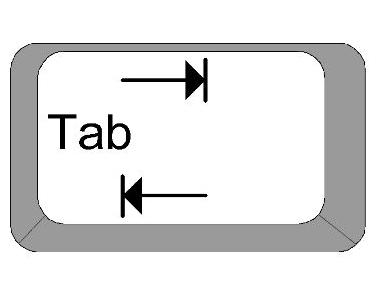
\includegraphics[scale=0.5]{../img/tab_key.jpg} para autocompletar las
  posibles rutas desde donde quiera que estes.
\item
  Escoge alguna (nuevamente usando la tecla tab para moverte entre las
  opciones). Si esto no funciona, teclea textualmente alguna de las
  rutas que ves.
\item
  Cierra la doble comilla y el paréntesis.
\item
  Teclea enter.
\item
  Debes encontrarte en la ruta elegida cuando tecleas \texttt{getwd()}.
\end{enumerate}

Con lo que acabamos de hacer, R buscará archivos o guardará archivos en
el folder \texttt{/home/animalito/study/}. En R también es posible
navegar a partir de el directorio de trabajo. Como siempre,

\begin{itemize}
\itemsep1pt\parskip0pt\parsep0pt
\item
  ``../un\_archivo.R'' le indica a R que busque un folder arriba del
  actual directorio de trabajo por el archivo \emph{un\_archivo.R}.
\item
  ``datos/otro\_archivo.R'' hace que se busque en el directorio de
  trabajo, dentro del folder \emph{datos} por el archivo
  \emph{otro\_archivo.R}
\end{itemize}

\begin{nota}
\textbf{Rutas relativas vs. Rutas absolutas\\}

El resultado que se muestra aquí al usar el comando \texttt{getwd()} depende de la computadora en la que se esta 
trabajando debido a que es una \textit{ruta absoluta}. Nota como es diferente la ruta 
que obtienes al correr el comando en tu consola de \texttt{R}. Eso es porque se trata 
de una ruta absoluta, es decir, es tal que da la ruta (\textit{path}) completo
al directorio en cuestión. Puedes accesar todos los directorios o archivos usando su ruta absoluta.\\

En investigación reproducible (\textit{reproducible research}), en investigación colaborativa o
incluso cuando trabajas en varias computadoras es una buena idea usar rutas relativas
en lugar de absolutas. Esto hace que el código sea menos dependiente de una estructura
de archivos o computadora en particular \parencite[][p. 67]{gandrud2013}. \\

En general, es \textit{buena práctica} configurar el código de un proyecto con rutas relativas.
En \texttt{R} en particular, cuando guardas un \texttt{Rmarkdown} y lo corres desde la línea de
comandos (o lo \textit{tejes} desde \texttt{RStudio}), la ruta que está fija -como si hubieras usado el comando \texttt{setwd()} es
en donde \textit{vive} ese archivo, es decir, el directorio en donde está guardado el mismo.\\

Desde cualquier \texttt{script} puedes llamar a otros usando este tipo de ruta como en 
el ejemplo anterior.
\end{nota}

\subsection{Ejemplos básicos}\label{ejemplos-basicos}

La consola permite hacer operaciones sobre números o caracteres (cuando
tiene sentido).

\begin{Shaded}
\begin{Highlighting}[]
\CommentTok{# Potencias, sumas, multiplicaciones}
\DecValTok{2}\NormalTok{^}\DecValTok{3} \NormalTok{+}\StringTok{ }\DecValTok{67} \NormalTok{*}\StringTok{ }\DecValTok{4} \NormalTok{-}\StringTok{ }\NormalTok{(}\DecValTok{45} \NormalTok{+}\StringTok{ }\DecValTok{5}\NormalTok{)}
\end{Highlighting}
\end{Shaded}

\begin{verbatim}
## [1] 226
\end{verbatim}

\begin{Shaded}
\begin{Highlighting}[]
\CommentTok{# Comparaciones}
\DecValTok{56} \NormalTok{>}\StringTok{ }\DecValTok{78} 
\end{Highlighting}
\end{Shaded}

\begin{verbatim}
## [1] FALSE
\end{verbatim}

\begin{Shaded}
\begin{Highlighting}[]
\DecValTok{34} \NormalTok{<=}\StringTok{ }\DecValTok{34}
\end{Highlighting}
\end{Shaded}

\begin{verbatim}
## [1] TRUE
\end{verbatim}

\begin{Shaded}
\begin{Highlighting}[]
\DecValTok{234} \NormalTok{<}\StringTok{ }\DecValTok{345}
\end{Highlighting}
\end{Shaded}

\begin{verbatim}
## [1] TRUE
\end{verbatim}

\begin{Shaded}
\begin{Highlighting}[]
\StringTok{"hola"} \NormalTok{==}\StringTok{ "hola"}
\end{Highlighting}
\end{Shaded}

\begin{verbatim}
## [1] TRUE
\end{verbatim}

\begin{Shaded}
\begin{Highlighting}[]
\StringTok{"buu"} \NormalTok{!=}\StringTok{ "yay"}
\end{Highlighting}
\end{Shaded}

\begin{verbatim}
## [1] TRUE
\end{verbatim}

\begin{Shaded}
\begin{Highlighting}[]
\CommentTok{# módulo}
\DecValTok{10} \NormalTok\StringTok{ }\DecValTok{4} 
\end{Highlighting}
\end{Shaded}

\begin{verbatim}
## [1] 2
\end{verbatim}

Estas operaciones también pueden ser realizadas entre vectores\footnote{Revisaremos
  más adelante con detalle la definición de vectores en la sección
  \ref{estructuras-de-datos}.}.

\begin{Shaded}
\begin{Highlighting}[]
\CommentTok{# Creamos un vector con entradas del -1 al 12 y lo asignamos a la variable x}
\NormalTok{x <-}\StringTok{ }\NormalTok{-}\DecValTok{1}\NormalTok{:}\DecValTok{12}
\CommentTok{# Lo vemos}
\NormalTok{x}
\end{Highlighting}
\end{Shaded}

\begin{verbatim}
##  [1] -1  0  1  2  3  4  5  6  7  8  9 10 11 12
\end{verbatim}

\begin{Shaded}
\begin{Highlighting}[]
\CommentTok{# Le sumamos 1 a todas las entradas}
\NormalTok{x +}\StringTok{ }\DecValTok{1}
\end{Highlighting}
\end{Shaded}

\begin{verbatim}
##  [1]  0  1  2  3  4  5  6  7  8  9 10 11 12 13
\end{verbatim}

\begin{Shaded}
\begin{Highlighting}[]
\CommentTok{# Multiplicamos por 2 cada entrada y le sumamos 3}
\DecValTok{2} \NormalTok{*}\StringTok{ }\NormalTok{x +}\StringTok{ }\DecValTok{3}
\end{Highlighting}
\end{Shaded}

\begin{verbatim}
##  [1]  1  3  5  7  9 11 13 15 17 19 21 23 25 27
\end{verbatim}

\begin{Shaded}
\begin{Highlighting}[]
\CommentTok{# Sacamos el módulo de cada entrada}
\NormalTok{x %%}\StringTok{ }\DecValTok{5} 
\end{Highlighting}
\end{Shaded}

\begin{verbatim}
##  [1] 4 0 1 2 3 4 0 1 2 3 4 0 1 2
\end{verbatim}

\subsection{Comandos útiles}\label{comandos-utiles}

Para enlistar los objetos que están en el espacio de trabajo

\begin{Shaded}
\begin{Highlighting}[]
\KeywordTok{ls}\NormalTok{()}
\end{Highlighting}
\end{Shaded}

\begin{verbatim}
## [1] "x"
\end{verbatim}

Para eliminar todos los objetos en un workspace

\begin{Shaded}
\begin{Highlighting}[]
\NormalTok{rm(list = ls(}\ErrorTok{))} \CommentTok{# se puede borrar solo uno, por ejemplo, nombrándolo}
\KeywordTok{ls}\NormalTok{()}
\end{Highlighting}
\end{Shaded}

\begin{verbatim}
## character(0)
\end{verbatim}

También se puede utilizar/guardar la historia de comandos utilizados

\begin{Shaded}
\begin{Highlighting}[]
\KeywordTok{history}\NormalTok{()}
\KeywordTok{history}\NormalTok{(}\DataTypeTok{max.show =} \DecValTok{5}\NormalTok{)}
\KeywordTok{history}\NormalTok{(}\DataTypeTok{max.show =} \OtherTok{Inf}\NormalTok{) }\CommentTok{# Muestra toda la historia}

\CommentTok{# Se puede salvar la historia de comandos a un archivo}
\KeywordTok{savehistory}\NormalTok{(}\DataTypeTok{file =} \StringTok{"mihistoria"}\NormalTok{) }\CommentTok{# Por default, R ya hace esto }
\CommentTok{# en un archivo ".Rhistory"}

\CommentTok{# Cargar al espacio de trabajo actual (current workspace) una }
\CommentTok{# historia de comandos en particular}
\KeywordTok{loadhistory}\NormalTok{(}\DataTypeTok{file =} \StringTok{"mihistoria"}\NormalTok{)}
\end{Highlighting}
\end{Shaded}

Es posible también guardar el workspace -en forma completa- en un
archivo con el comando \texttt{save.image()} a un archivo con extensión
\emph{.RData}. Puedes guardar una lista de objetos específica a un
archivo \emph{.RData}. Por ejemplo:

\begin{Shaded}
\begin{Highlighting}[]
\NormalTok{x <-}\StringTok{ }\DecValTok{1}\NormalTok{:}\DecValTok{12}
\NormalTok{y <-}\StringTok{ }\DecValTok{3}\NormalTok{:}\DecValTok{45}
\NormalTok{save(x, y, file = }\StringTok{"ejemplo.RData"}\ErrorTok{)} \CommentTok{#la extensión puede ser arbitraria.}
\end{Highlighting}
\end{Shaded}

Después puedo cargar ese archivo. Prueba hacer:

\begin{Shaded}
\begin{Highlighting}[]
\KeywordTok{rm}\NormalTok{(}\DataTypeTok{list =} \KeywordTok{ls}\NormalTok{()) }\CommentTok{# limpiamos workspace}
\NormalTok{load(file = }\StringTok{"ejemplo.RData"}\ErrorTok{)} \CommentTok{#la extensión puede ser arbitraria.}
\KeywordTok{ls}\NormalTok{()}
\end{Highlighting}
\end{Shaded}

Nota como los objetos preservan el nombre con el que fueron guardados.

\section{Paquetes (\emph{libraries})}\label{paquetes-libraries}

R puede hacer muchos análisis estadísticos y de datos. Las diferentes
capacidades están organizadas en paquetes o librerías. Con la
instalación estándar resumida en la sección \ref{instalacion}, se
instalan también los paquetes más comunes (también llamado el
\emph{base} o R-básico). Para obtener una lista de todos los paquetes
instalados se puede utilizar el comando \texttt{library()} en la consola
o en un script.

Existen una gran cantidad de paquetes disponibles además de los
incluidos por omisión (\emph{default}).

\subsection{CRAN}\label{cran}

\emph{Comprehensive R Archive Network} \parencite{cran} es una colección
de sitios que contienen exactamente el mismo material, es decir, son
espejos (\emph{mirrors}) de las distribuciones de R, las extensiones, la
documentación y los binarios. El master de CRAN está en
Wirtschaftsuniversität Wien en Austria. Éste se ``espeja''
(\emph{mirrors}) en forma diaria a muchos sitios alrededor del mundo. En
la \href{https://cran.r-project.org/mirrors.html}{lista de espejos} se
puede ver que para México están disponibles el espejo del ITAM, del
Colegio de Postgraduados (Texcoco) y Jellyfish Foundation
\parencite{cran}.

Los espejos son importantes pues, cada vez que busquen instalar
paquetes, se les preguntará qué espejo quieren utilizar para la sesión
en cuestión. Del espejo que selecciones, será del cuál R \emph{bajará}
el binario y la documentación.

Del CRAN es que se obtiene la última versión oficial de R. Diario se
actualizan los espejos. Para más detalles consultar el
\href{https://cran.r-project.org/doc/FAQ/R-FAQ.html}{FAQ}.

Para contribuir un paquete en CRAN se deben seguir las instrucciones
\href{https://cran.r-project.org/web/packages/policies.html}{aquí}.

\subsection{Github}\label{github}

Git es un controlador de versiones muy popular para desarrollar
software. Cuando se combina con \href{https://github.com/}{GitHub} se
puede compartir el código con el resto de la comunidad. Éste controlador
de versiones es el más popular entre los que contribuyen a R. Muchos
problemas a los que uno se enfrenta alguien ya los desarrolló y no
necesariamente publicó el paquete en CRAN. Para instalar algún paquete
desde GitHub, se pueden seguir las instrucciones siguientes

\begin{Shaded}
\begin{Highlighting}[]
\KeywordTok{install.packages}\NormalTok{(}\StringTok{"devtools"}\NormalTok{)}
\NormalTok{devtools::}\KeywordTok{install_github}\NormalTok{(}\StringTok{"username/packagename"}\NormalTok{)}
\end{Highlighting}
\end{Shaded}

Donde \texttt{username} es el usuario de Github y \texttt{packagename}
es el nombre del repositorio que contiene el paquete. Cuidado, no todo
repositorio en GitHub es un paquete. Para más información ver el
capítulo \href{http://r-pkgs.had.co.nz/git.html}{Git and GitHub} en
\textcite{wickham2015r}.

\subsection{Otras fuentes}\label{otras-fuentes}

Otros lugares en donde es común que se publiquen paquetes es en
\href{https://www.bioconductor.org/}{Bioconductor} un projecto de
software para la comprensión de datos del genoma humano.

\section{Paquetes recomendados}\label{paquetes-recomendados}

Hay muchísimas librerías y lo recomendable es, dado un problema y un
modelo para resolverlo, revisar si alguien ya implementó el método en
algunas de las fuentes de paquetes mencionadas antes.

Para mantener orden en los paquetes descargados puede ser útil utilizar
el \textcite{pacman} pues provee de herramientas para instalar paquetes
en una forma un poco más sencilla que usando la función
\texttt{install.packages}.

En particular, la función \texttt{p\_load} permite instalar, cargar y
actualizar uno o varios paquetes.

Si queremos instalar varios paquetes usando las herramientas del R
básico (\emph{base}) \parencite{rbase} haríamos algo como
\parencite[ejemplo tomado de][en la viñeta de intrducción al paquete]{pacman}:

\begin{Shaded}
\begin{Highlighting}[]
\NormalTok{packs <-}\StringTok{ }\KeywordTok{c}\NormalTok{(}\StringTok{"XML"}\NormalTok{, }\StringTok{"devtools"}\NormalTok{, }\StringTok{"RCurl"}\NormalTok{, }\StringTok{"fakePackage"}\NormalTok{, }\StringTok{"SPSSemulate"}\NormalTok{)}
\NormalTok{success <-}\StringTok{ }\KeywordTok{suppressWarnings}\NormalTok{(}\KeywordTok{sapply}\NormalTok{(packs, require, }\DataTypeTok{character.only =} \OtherTok{TRUE}\NormalTok{))}
\KeywordTok{install.packages}\NormalTok{(}\KeywordTok{names}\NormalTok{(success)[!success])}
\KeywordTok{sapply}\NormalTok{(}\KeywordTok{names}\NormalTok{(success)[!success], require, }\DataTypeTok{character.only =} \OtherTok{TRUE}\NormalTok{)}
\end{Highlighting}
\end{Shaded}

Con \texttt{pacman::p\_load} la tarea se reduce a:

\begin{Shaded}
\begin{Highlighting}[]
\NormalTok{pacman::}\KeywordTok{p_load}\NormalTok{(XML, devtools, RCurl, fakePackage, SPSSemulate)}
\end{Highlighting}
\end{Shaded}

\begin{curiosidad}
Nota como se puede llamar a una función por su nombre \texttt{p\_load} una vez que 
ya cargamos el paquete en el cuál esa función está guardada con el comando \texttt{library(pacman)}
o podemos llamarla directamente utilizando la convención \texttt{paquete::funcion}, en este caso,
\texttt{pacman::p\_load}.
\end{curiosidad}

Para instalar \texttt{pacman} escribe:

\begin{Shaded}
\begin{Highlighting}[]
\KeywordTok{install.packages}\NormalTok{(}\StringTok{"pacman"}\NormalTok{)}
\end{Highlighting}
\end{Shaded}

Algunos paquetes se encuentran en desarrollo. En particular, si se
encuentran en \texttt{github} pueden descargarse usando la función
\texttt{pacman::p\_install\_gh('usuario/repositorio')}.

A continuación, hay una lista de paquetes que se recomienda descargar o
revisar para tener a la mano herramientas diversas útiles para el
trabajo del científico de datos. La lista no es comprensiva pues hay un
gran número de paquetes útiles.

\begin{Shaded}
\begin{Highlighting}[]
\CommentTok{# Para cargar datos al ambiente de trabajo (data load)}
\NormalTok{pacman::}\KeywordTok{p_load}\NormalTok{(RODBC, RMySQL, RPostgreSQL, RSQLite, foreign, Rpostgres, haven}
               \NormalTok{, readr)}
\NormalTok{pacman::}\KeywordTok{p_install_gh}\NormalTok{(}\StringTok{"hadley/readxl"}\NormalTok{)}
\NormalTok{pacman::}\KeywordTok{p_install_gh}\NormalTok{(}\StringTok{"rstats-db/RPostgres"}\NormalTok{)}

\CommentTok{# Para manipular datos (data manipulation)}
\NormalTok{pacman::}\KeywordTok{p_load}\NormalTok{(plyr, dplyr, data.table, tidyr, stringr, lubridate, gsubfn)}

\CommentTok{# Para visualizar datos (data visualization)}
\NormalTok{pacman::}\KeywordTok{p_load}\NormalTok{(ggplot2, graphics, ggvis)}
\NormalTok{pacman::}\KeywordTok{p_install_gh}\NormalTok{(}\StringTok{"RcppCore/Rcpp"}\NormalTok{)}
\NormalTok{pacman::}\KeywordTok{p_install_gh}\NormalTok{(}\StringTok{"rstats-db/DBI"}\NormalTok{)}
\NormalTok{pacman::}\KeywordTok{p_install_gh}\NormalTok{(}\StringTok{'ramnathv/htmlwidgets'}\NormalTok{)}
\NormalTok{pacman::}\KeywordTok{p_install_gh}\NormalTok{(}\StringTok{'rstudio/leaflet'}\NormalTok{)}
\NormalTok{pacman::}\KeywordTok{p_install_gh}\NormalTok{(}\StringTok{'bwlewis/rthreejs'}\NormalTok{)}
\NormalTok{pacman::}\KeywordTok{p_install_gh}\NormalTok{(}\StringTok{'htmlwidgets/sparkline'}\NormalTok{)}
\NormalTok{pacman::}\KeywordTok{p_load}\NormalTok{(dygraphs, DT, DiagrammeR, networkD3, googleVis)}

\CommentTok{# Para modelar (data modelling)}
\NormalTok{pacman::}\KeywordTok{p_load}\NormalTok{(car, mgcv, lme4, nlme, randomForest, multcomp, vcd, glmnet, survival, caret)}

\CommentTok{# Para generar reportes (reports)}
\NormalTok{pacman::}\KeywordTok{p_load}\NormalTok{(shiny, xtable, knitr, rmarkdown)}

\CommentTok{# Para trabajar con datos espaciales (spatial data)}
\NormalTok{pacman::}\KeywordTok{p_load}\NormalTok{(sp, maptools, maps, ggmap, rgdal)}

\CommentTok{# Para trabajo con series de tiempo (time series)}
\NormalTok{pacman::}\KeywordTok{p_load}\NormalTok{(zoo, quantmod)}

\CommentTok{# Para escribir código de alto rendimiento en R (High performance R code)}
\NormalTok{pacman::}\KeywordTok{p_load}\NormalTok{(Rcpp, parallel)}

\CommentTok{# Trabajar con la web }
\NormalTok{pacman::}\KeywordTok{p_load}\NormalTok{(XML, jsonlite, httr)}

\CommentTok{# Para escribir paquetes en R}
\NormalTok{pacman::}\KeywordTok{p_load}\NormalTok{(devtools, testthat, roxygen2)}
\end{Highlighting}
\end{Shaded}

\section{Scripting}\label{scripting}

R es un intérprete. Utiliza un ambiente basado en línea de comandos. Por
ende, es necesario escribir la secuencia de comandos que se desea
realizar a diferencia de otras herramientas en donde es posible utlizar
el mouse o menús.

Aunque los comandos pueden ser ejecutados directamente en consola una
única vez, también es posible guardarlos en archivos conocidos como
\emph{scripts}. Típicamente, utilizamos la extensión \textbf{.R} o
\textbf{.r}. En RStudio \parencite{rstudio}, \texttt{CTRL + SHIFT + N}
abre inmediatamente un nuevo editor en el panel superior izquierdo.

En RStudio, por ejemplo, se puede \emph{ir editando} el script y
corriendo los comandos línea por línea con \texttt{CTRL + ENTER}. Esto
también aplica para \emph{correr} una selección del texto
editable\footnote{RStudio tiene muchos
  \href{https://support.rstudio.com/hc/en-us/articles/200711853-Keyboard-Shortcuts}{atajos
  de teclado} que facilitan el trabajo.}.

Es posible también correr todo el script

\begin{Shaded}
\begin{Highlighting}[]
\KeywordTok{source}\NormalTok{(}\StringTok{"foo.R"}\NormalTok{)}
\end{Highlighting}
\end{Shaded}

O con el atajo \texttt{CTRL + SHIFT + S} en RStudio.

Para enlistar algunos shortcuts comunes en RStudio presiona
\texttt{ALT + SHIFT + K}.

De la misma manera, si utilizas \texttt{Emacs + ESS}
\parencite{rossini2004ess}, existen múltiples atajos de teclado para
realizar todo mucho más eficientemente. Estudiarlos no es tiempo
perdido.

\section{Ayuda y documentación}\label{ayuda-y-documentacion}

\texttt{R} tiene mucha documentación. Dado que es imposible recordar
todas las funciones o cómo utilizar todo lo que ya está hecho, es
necesario aprender a leerla. Desde la consola se puede accesar a la
misma.

Para ayuda general,

\begin{Shaded}
\begin{Highlighting}[]
\KeywordTok{help.start}\NormalTok{()}
\end{Highlighting}
\end{Shaded}

Para la \textbf{ayuda de una función en especifico}, por ejemplo, si se
quiere graficar algo y sabemos que existe la funcion \texttt{plot}
podemos consultar fácilmente la ayuda.

\begin{Shaded}
\begin{Highlighting}[]
\KeywordTok{help}\NormalTok{(plot)}
\CommentTok{# o tecleando directamente}
\NormalTok{?plot}
\end{Highlighting}
\end{Shaded}

El segundo ejemplo se puede extender para buscar esa función en todos
los paquetes que tengo instalados en mi ambiente al escribir
\texttt{??plot}.

A veces, es útil ver el \textbf{cuerpo de una función}. Esta tarea no
necesariamente es trivial. Para funciones generadas por el usuario, usa

\begin{Shaded}
\begin{Highlighting}[]
\NormalTok{xx <-}\StringTok{ }\NormalTok{function(x) x^}\DecValTok{2}
\KeywordTok{body}\NormalTok{(xx)}
\end{Highlighting}
\end{Shaded}

\begin{verbatim}
## x^2
\end{verbatim}

\begin{Shaded}
\begin{Highlighting}[]
\CommentTok{# o simplemente imprimir el objeto en donde guardamos la función}
\NormalTok{xx}
\end{Highlighting}
\end{Shaded}

\begin{verbatim}
## function(x) x^2
\end{verbatim}

También funciona para algunas funciones de paquete, por ejemplo
\texttt{rename}:

\begin{Shaded}
\begin{Highlighting}[]
\KeywordTok{library}\NormalTok{(plyr)}
\KeywordTok{body}\NormalTok{(rename)}
\end{Highlighting}
\end{Shaded}

\begin{verbatim}
## {
##     names(x) <- revalue(names(x), replace, warn_missing = warn_missing)
##     duplicated_names <- names(x)[duplicated(names(x))]
##     if (warn_duplicated && (length(duplicated_names) > 0L)) {
##         duplicated_names_message <- paste0("`", duplicated_names, 
##             "`", collapse = ", ")
##         warning("The plyr::rename operation has created duplicates for the ", 
##             "following name(s): (", duplicated_names_message, 
##             ")", call. = FALSE)
##     }
##     x
## }
\end{verbatim}

Para plot, en cambio, al usar la función \texttt{body} se ve:

\begin{Shaded}
\begin{Highlighting}[]
\KeywordTok{body}\NormalTok{(plot)}
\end{Highlighting}
\end{Shaded}

\begin{verbatim}
## UseMethod("plot")
\end{verbatim}

Esto es porque \texttt{plot} es una función genérica (S3) que tiene
métodos para distintas clases de objetos. En esos casos, primero debemos
usar la función \texttt{methods} para enlistar los métodos que tiene esa
función.

\begin{Shaded}
\begin{Highlighting}[]
\KeywordTok{methods}\NormalTok{(plot)}
\end{Highlighting}
\end{Shaded}

\begin{verbatim}
##  [1] plot.acf*           plot.data.frame*    plot.decomposed.ts*
##  [4] plot.default        plot.dendrogram*    plot.density*      
##  [7] plot.ecdf           plot.factor*        plot.formula*      
## [10] plot.function       plot.hclust*        plot.histogram*    
## [13] plot.HoltWinters*   plot.isoreg*        plot.lm*           
## [16] plot.medpolish*     plot.mlm*           plot.ppr*          
## [19] plot.prcomp*        plot.princomp*      plot.profile.nls*  
## [22] plot.raster*        plot.spec*          plot.stepfun       
## [25] plot.stl*           plot.table*         plot.ts            
## [28] plot.tskernel*      plot.TukeyHSD*     
## see '?methods' for accessing help and source code
\end{verbatim}

Si tiene asteriscos, significa que la función para ese método en
particular no viene directamente del espacio de nombres del paquete
pero, de cualquier forma, lo podemos pedir usando la
\texttt{función getAnywhere} para cualquiera de los métodos que se
desplegaron:

\begin{Shaded}
\begin{Highlighting}[]
\KeywordTok{getAnywhere}\NormalTok{(plot.density)}
\end{Highlighting}
\end{Shaded}

\begin{verbatim}
## A single object matching 'plot.density' was found
## It was found in the following places
##   registered S3 method for plot from namespace stats
##   namespace:stats
## with value
## 
## function (x, main = NULL, xlab = NULL, ylab = "Density", type = "l", 
##     zero.line = TRUE, ...) 
## {
##     if (is.null(xlab)) 
##         xlab <- paste("N =", x$n, "  Bandwidth =", formatC(x$bw))
##     if (is.null(main)) 
##         main <- deparse(x$call)
##     plot.default(x, main = main, xlab = xlab, ylab = ylab, type = type, 
##         ...)
##     if (zero.line) 
##         abline(h = 0, lwd = 0.1, col = "gray")
##     invisible(NULL)
## }
## <bytecode: 0x1ea9370>
## <environment: namespace:stats>
\end{verbatim}

Nota como el método \texttt{plot.density} viene del paquete
\texttt{stats}
\footnote{Hay otro tipo de funciones en las accesar al código fuente no se pueda con los métodos descritos. Para ello, es útil revisar la sección "old-school object-oriented programming in R" \parencite[][p.131-133]{adler2010r} o las secciones dedicadas a los objetos S3 y S4 en \textcite{wickham2014advanced}.}.

La documentación normalmente se acompaña de \textbf{ejemplos}. Para
\emph{correr} los ejemplos sin necesidad de copiar y pegar, prueba

\begin{Shaded}
\begin{Highlighting}[]
\KeywordTok{example}\NormalTok{(plot)}
\end{Highlighting}
\end{Shaded}

Para búsquedas más comprensivas, se puede buscar de otras maneras:

\begin{Shaded}
\begin{Highlighting}[]
\KeywordTok{apropos}\NormalTok{(}\StringTok{"foo"}\NormalTok{) }\CommentTok{# Enlista todas las funciones que contengan la cadena "foo"}
\KeywordTok{RSiteSearch}\NormalTok{(}\StringTok{"foo"}\NormalTok{) }\CommentTok{# Busca por la cadena "foo" en todos los manuales de ayuda }
\CommentTok{# y listas de distribución.}
\end{Highlighting}
\end{Shaded}

\section{Optimizando}\label{optimizando}

Es común que muy pronto nos encontremos con limitaciones al poder de
cómputo y rapidez con el que R procesa los datos. Hay operaciones
intensivas como, por ejemplo, la inversión de matrices (qr) o el
análisis por componentes principales (svd). Incluso una selección de
variables (\emph{back/forward selection}) usando una simple regresión
lineal sobre múltiples regresores puede llevar un tiempo de cómputo de
horas/días o no terminar.

Una de las manera más rápidas de mejorar el performance de \texttt{R} es
instalando las librerías de álgebra lineal que puede utilizar el
software para hacer las operaciones más rápido.

Para mucho (demasiado) detalle al respecto, referirse a la comparación
de performance en \textcite{eddelbuettel2010} o al paquete del mismo
autor \textcite{gcbd}.

Para la parte práctica de todo esto, referirse a
\href{http://brettklamer.com/diversions/statistical/faster-blas-in-r/}{este
blog} para instalar las librerías apropiadas para BLAS y Lapack
\parencite{blasinr}. Para una comparación bastante práctica de las
diferentes versiones de esas librerías, ver
\href{http://blog.nguyenvq.com/blog/2014/11/10/optimized-r-and-python-standard-blas-vs-atlas-vs-openblas-vs-mkl/}{aquí}
\parencite{optimizedr}.

\end{document}
 

\chapter{Estructuras y funciones}
\graphicspath{{01_programacion_basica/}}
\documentclass[]{article}
\usepackage{lmodern}
\usepackage{amssymb,amsmath}
\usepackage{ifxetex,ifluatex}
\usepackage{fixltx2e} % provides \textsubscript
\ifnum 0\ifxetex 1\fi\ifluatex 1\fi=0 % if pdftex
  \usepackage[T1]{fontenc}
  \usepackage[utf8]{inputenc}
\else % if luatex or xelatex
  \ifxetex
    \usepackage{mathspec}
  \else
    \usepackage{fontspec}
  \fi
  \defaultfontfeatures{Ligatures=TeX,Scale=MatchLowercase}
\fi
% use upquote if available, for straight quotes in verbatim environments
\IfFileExists{upquote.sty}{\usepackage{upquote}}{}
% use microtype if available
\IfFileExists{microtype.sty}{%
\usepackage{microtype}
\UseMicrotypeSet[protrusion]{basicmath} % disable protrusion for tt fonts
}{}
\usepackage[margin=1in]{geometry}
\usepackage{hyperref}
\hypersetup{unicode=true,
            pdftitle={Estructuras y funciones},
            pdfborder={0 0 0},
            breaklinks=true}
\urlstyle{same}  % don't use monospace font for urls
\usepackage{color}
\usepackage{fancyvrb}
\newcommand{\VerbBar}{|}
\newcommand{\VERB}{\Verb[commandchars=\\\{\}]}
\DefineVerbatimEnvironment{Highlighting}{Verbatim}{commandchars=\\\{\}}
% Add ',fontsize=\small' for more characters per line
\usepackage{framed}
\definecolor{shadecolor}{RGB}{248,248,248}
\newenvironment{Shaded}{\begin{snugshade}}{\end{snugshade}}
\newcommand{\KeywordTok}[1]{\textcolor[rgb]{0.13,0.29,0.53}{\textbf{#1}}}
\newcommand{\DataTypeTok}[1]{\textcolor[rgb]{0.13,0.29,0.53}{#1}}
\newcommand{\DecValTok}[1]{\textcolor[rgb]{0.00,0.00,0.81}{#1}}
\newcommand{\BaseNTok}[1]{\textcolor[rgb]{0.00,0.00,0.81}{#1}}
\newcommand{\FloatTok}[1]{\textcolor[rgb]{0.00,0.00,0.81}{#1}}
\newcommand{\ConstantTok}[1]{\textcolor[rgb]{0.00,0.00,0.00}{#1}}
\newcommand{\CharTok}[1]{\textcolor[rgb]{0.31,0.60,0.02}{#1}}
\newcommand{\SpecialCharTok}[1]{\textcolor[rgb]{0.00,0.00,0.00}{#1}}
\newcommand{\StringTok}[1]{\textcolor[rgb]{0.31,0.60,0.02}{#1}}
\newcommand{\VerbatimStringTok}[1]{\textcolor[rgb]{0.31,0.60,0.02}{#1}}
\newcommand{\SpecialStringTok}[1]{\textcolor[rgb]{0.31,0.60,0.02}{#1}}
\newcommand{\ImportTok}[1]{#1}
\newcommand{\CommentTok}[1]{\textcolor[rgb]{0.56,0.35,0.01}{\textit{#1}}}
\newcommand{\DocumentationTok}[1]{\textcolor[rgb]{0.56,0.35,0.01}{\textbf{\textit{#1}}}}
\newcommand{\AnnotationTok}[1]{\textcolor[rgb]{0.56,0.35,0.01}{\textbf{\textit{#1}}}}
\newcommand{\CommentVarTok}[1]{\textcolor[rgb]{0.56,0.35,0.01}{\textbf{\textit{#1}}}}
\newcommand{\OtherTok}[1]{\textcolor[rgb]{0.56,0.35,0.01}{#1}}
\newcommand{\FunctionTok}[1]{\textcolor[rgb]{0.00,0.00,0.00}{#1}}
\newcommand{\VariableTok}[1]{\textcolor[rgb]{0.00,0.00,0.00}{#1}}
\newcommand{\ControlFlowTok}[1]{\textcolor[rgb]{0.13,0.29,0.53}{\textbf{#1}}}
\newcommand{\OperatorTok}[1]{\textcolor[rgb]{0.81,0.36,0.00}{\textbf{#1}}}
\newcommand{\BuiltInTok}[1]{#1}
\newcommand{\ExtensionTok}[1]{#1}
\newcommand{\PreprocessorTok}[1]{\textcolor[rgb]{0.56,0.35,0.01}{\textit{#1}}}
\newcommand{\AttributeTok}[1]{\textcolor[rgb]{0.77,0.63,0.00}{#1}}
\newcommand{\RegionMarkerTok}[1]{#1}
\newcommand{\InformationTok}[1]{\textcolor[rgb]{0.56,0.35,0.01}{\textbf{\textit{#1}}}}
\newcommand{\WarningTok}[1]{\textcolor[rgb]{0.56,0.35,0.01}{\textbf{\textit{#1}}}}
\newcommand{\AlertTok}[1]{\textcolor[rgb]{0.94,0.16,0.16}{#1}}
\newcommand{\ErrorTok}[1]{\textcolor[rgb]{0.64,0.00,0.00}{\textbf{#1}}}
\newcommand{\NormalTok}[1]{#1}
\usepackage{longtable,booktabs}
\usepackage{graphicx,grffile}
\makeatletter
\def\maxwidth{\ifdim\Gin@nat@width>\linewidth\linewidth\else\Gin@nat@width\fi}
\def\maxheight{\ifdim\Gin@nat@height>\textheight\textheight\else\Gin@nat@height\fi}
\makeatother
% Scale images if necessary, so that they will not overflow the page
% margins by default, and it is still possible to overwrite the defaults
% using explicit options in \includegraphics[width, height, ...]{}
\setkeys{Gin}{width=\maxwidth,height=\maxheight,keepaspectratio}
\IfFileExists{parskip.sty}{%
\usepackage{parskip}
}{% else
\setlength{\parindent}{0pt}
\setlength{\parskip}{6pt plus 2pt minus 1pt}
}
\setlength{\emergencystretch}{3em}  % prevent overfull lines
\providecommand{\tightlist}{%
  \setlength{\itemsep}{0pt}\setlength{\parskip}{0pt}}
\setcounter{secnumdepth}{5}
% Redefines (sub)paragraphs to behave more like sections
\ifx\paragraph\undefined\else
\let\oldparagraph\paragraph
\renewcommand{\paragraph}[1]{\oldparagraph{#1}\mbox{}}
\fi
\ifx\subparagraph\undefined\else
\let\oldsubparagraph\subparagraph
\renewcommand{\subparagraph}[1]{\oldsubparagraph{#1}\mbox{}}
\fi

%%% Use protect on footnotes to avoid problems with footnotes in titles
\let\rmarkdownfootnote\footnote%
\def\footnote{\protect\rmarkdownfootnote}

%%% Change title format to be more compact
\usepackage{titling}

% Create subtitle command for use in maketitle
\newcommand{\subtitle}[1]{
  \posttitle{
    \begin{center}\large#1\end{center}
    }
}

\setlength{\droptitle}{-2em}
  \title{Estructuras y funciones}
  \pretitle{\vspace{\droptitle}\centering\huge}
  \posttitle{\par}
  \author{}
  \preauthor{}\postauthor{}
  \date{}
  \predate{}\postdate{}

\usepackage[
  backend=biber,
  style=alphabetic,
  sorting=ynt,
  citestyle=authoryear
  ]{biblatex}
\addbibresource{../lit/bib.bib}

\usepackage[utf8]{inputenc}
\usepackage[spanish]{babel}

\usepackage{float}
\usepackage{enumitem}
\newcommand\novspace{\@minipagetrue}

%%%% Frames
\ifxetex
    \makeatletter % undo the wrong changes made by mathspec
    \let\RequirePackage\original@RequirePackage
    \let\usepackage\RequirePackage
    \makeatother
\fi

\usepackage{xcolor}
\usepackage[tikz]{bclogo}
\usepackage[framemethod=tikz]{mdframed}
\usepackage{lipsum}
\usepackage[many]{tcolorbox}

\definecolor{bgblue}{RGB}{245,243,253}
\definecolor{ttblue}{RGB}{91,194,224}
\definecolor{llred}{RGB}{255,228,225}
\definecolor{bbblack}{RGB}{0,0,0}

\mdfdefinestyle{mystyle}{%
  rightline=true,
  innerleftmargin=10,
  innerrightmargin=10,
  outerlinewidth=3pt,
  topline=false,
  rightline=true,
  bottomline=false,
  skipabove=\topsep,
  skipbelow=\topsep
}

\newtcolorbox{curiosidad}[1][]{
  breakable,
  title=#1,
  colback=white,
  colbacktitle=white,
  coltitle=black,
  fonttitle=\bfseries,
  bottomrule=0pt,
  toprule=0pt,
  leftrule=3pt,
  rightrule=3pt,
  titlerule=0pt,
  arc=0pt,
  outer arc=0pt,
  colframe=black,
}

\newtcolorbox{nota}[1][]{
  breakable,
  freelance,
  title=#1,
  colback=white,
  colbacktitle=white,
  coltitle=black,
  fonttitle=\bfseries,
  bottomrule=0pt,
  boxrule=0pt,
  colframe=white,
  overlay unbroken and first={
  \draw[red!75!black,line width=3pt]
    ([xshift=5pt]frame.north west) -- 
    (frame.north west) -- 
    (frame.south west);
  \draw[red!75!black,line width=3pt]
    ([xshift=-5pt]frame.north east) -- 
    (frame.north east) -- 
    (frame.south east);
  },
  overlay unbroken app={
  \draw[red!75!black,line width=3pt,line cap=rect]
    (frame.south west) -- 
    ([xshift=5pt]frame.south west);
  \draw[red!75!black,line width=3pt,line cap=rect]
    (frame.south east) -- 
    ([xshift=-5pt]frame.south east);
  },
  overlay middle and last={
  \draw[red!75!black,line width=3pt]
    (frame.north west) -- 
    (frame.south west);
  \draw[red!75!black,line width=3pt]
    (frame.north east) -- 
    (frame.south east);
  },
  overlay last app={
  \draw[red!75!black,line width=3pt,line cap=rect]
    (frame.south west) --
    ([xshift=5pt]frame.south west);
  \draw[red!75!black,line width=3pt,line cap=rect]
    (frame.south east) --
    ([xshift=-5pt]frame.south east);
  },
}

\begin{document}


En este capítulo se introducen los principales objetos de \texttt{R}.
Primero, se definen brevemente. Después se introducen las funciones,
objetos que permiten realizar acciones sobre otros objetos.

Posteriormente, se introducen las distintas estructuras de datos en
\texttt{R} básico. El primer bloque de construcción son las
\emph{clases} de datos con los que \texttt{R} sabe trabajar, es decir,
caracteres, números enteros, reales, complejos y booleanos.

El segundo bloque son los \emph{vectores}. Esta es una estructura
fundamental en \texttt{R} y están conformados por un conjunto de
elementos de una de las clases de datos. El tercero son las
\emph{matrices}, que le agregan una dimensión a los vectores. Las
\emph{listas} son como vectores pero pueden contener un subconjunto de
elementos de cualesquiera de las clases, incluida otra lista.

Los \emph{dataframes} son listas con la restricción que cada uno de sus
elementos es un vector del mismo tamaño. Esta estructura es la más
natural para un estadístico pues refiere a la forma tabular en la que se
acostumbra pensar a los datos en esa disciplina. Los \emph{tibbles} y
los \emph{datatables} extienden los dataframes, haciéndolos más
eficientes para el procesamiento de una mayor cantidad de datos.

Finalmente, se mencionan objetos adicionales -como el infinito y el
objeto que representa valores perdidos- y se describen las principales
estructuras de control, proporcionando ejemplos para escribirlos en
\texttt{R}.

\section{Objetos}\label{objetos}

\renewcommand\bcStyleTitre[1]{\large\textcolor{ttblue}{#1}}

\begin{bclogo}[
  couleur=bgblue,
  arrondi=0,
  logo=\bcattention,
  barre=none,
  noborder=true]{En R}
\begin{itemize}
\item Todo lo que existe es un objeto.
\item Todo lo que sucede es una llamada a una función.
\end{itemize}
\end{bclogo}

Todo lenguaje de programación provee de una forma de accesar los datos
guardados en memoria. R no permite un acceso directo a la memoria de la
computadora pero ofrece varias estructuras de datos especializadas para
realizar esa tarea. A estas estructuras, se les da el nombre de objetos
\parencite[][ver sección 2 ``objetos'']{rmanual}. Estos objetos son
referidos a través de símbolos o variables, sin embargo, los símbolos
son también objetos y pueden ser manipulados de la misma manera.

Todos los objetos tienen un \emph{tipo}, mismo que se le puede preguntar
a los objetos con la función \texttt{typeof}

\begin{Shaded}
\begin{Highlighting}[]
\KeywordTok{typeof}\NormalTok{(}\StringTok{"hola"}\NormalTok{)}
\end{Highlighting}
\end{Shaded}

\begin{verbatim}
## [1] "character"
\end{verbatim}

Esta función puede reconocer muchos tipos, entre ellos algunos de los
que veremos con mayor detalle a continuación. Comenzaremos con las
funciones que, regresando al cuadro anterior, \emph{todo lo que sucede
es una llamada a una función}. Posteriormente, se revisarán las
estructuras de datos más básicas en R y, por último, se verán
estructuras de control básicas que permitirán mezclar el uso de objetos
de manera que se operen bajo ciertas condiciones lógicas.

\section{Funciones}\label{funciones}

Hay una regla de oro en programación en general: \emph{DRY
code}\footnote{El concepto es mucho más general que esto pero lo
  reduciremos a una de sus capas más bajas primero para introducirlo y,
  segundo, porque el concepto general cobra sentido al avanzar en las
  tareas de programación a las que se enfrenta el usuario.} (acrónimo de
``Don't repeat yourself'') \parencite{hunt2000}. Básicamente esto se
reduce a \emph{no te repitas}. Cuando tienes las mismas líneas de código
varias veces (cuando estas copiando y pegando mucho) entonces lo que
necesitas es escribir una función que realice esa tarea.

En R las funciones son los \emph{building blocks} de básicamente todo.
Como todo lo demás en R, las funciones son también objetos. Cuando
llamas a un objeto en R, casi siempre estas en realidad llamando a una
función.

\subsection{Componentes de una
función}\label{componentes-de-una-funcion}

\begin{itemize}
\tightlist
\item
  El \texttt{body()} o cuerpo de la función es el código dentro de la
  misma.
\item
  \texttt{formals()} o el listado de argumentos formales de la función,
  controla cómo se puede llamar a una función.
\item
  El ambiente \texttt{environment()} determina cómo son referidas las
  variables dentro de la función.
\item
  La lista de argumentos se obtiene con \texttt{args()}
\end{itemize}

\begin{Shaded}
\begin{Highlighting}[]
\CommentTok{# Ejecuto la función}
\NormalTok{f <-}\StringTok{ }\ControlFlowTok{function}\NormalTok{(x) x}
\CommentTok{# Imprimo el objeto f}
\NormalTok{f}
\end{Highlighting}
\end{Shaded}

\begin{verbatim}
## function(x) x
\end{verbatim}

\begin{Shaded}
\begin{Highlighting}[]
\CommentTok{# Al usar la función body, veo solo el cuerpo}
\KeywordTok{body}\NormalTok{(f)}
\end{Highlighting}
\end{Shaded}

\begin{verbatim}
## x
\end{verbatim}

\begin{Shaded}
\begin{Highlighting}[]
\CommentTok{# Listo sus parámetros o argumentos}
\KeywordTok{formals}\NormalTok{(f)}
\end{Highlighting}
\end{Shaded}

\begin{verbatim}
## $x
\end{verbatim}

\begin{Shaded}
\begin{Highlighting}[]
\CommentTok{# Veo en qué ambiente está la función}
\KeywordTok{environment}\NormalTok{(f)}
\end{Highlighting}
\end{Shaded}

\begin{verbatim}
## <environment: R_GlobalEnv>
\end{verbatim}

Una vez definida una función, llamarla es muy sencillo: se le
proporciona un valor para los parámetros y nos regresa el resultado
esperado. Una función puede regresar cualquier objeto, por ejemplo, una
función o un valor. Llamamos a la función declarada arriba:

\begin{Shaded}
\begin{Highlighting}[]
\KeywordTok{f}\NormalTok{(}\DecValTok{4}\NormalTok{)}
\end{Highlighting}
\end{Shaded}

\begin{verbatim}
## [1] 4
\end{verbatim}

\begin{Shaded}
\begin{Highlighting}[]
\CommentTok{# Elimino la función del espacio de trabajo}
\KeywordTok{rm}\NormalTok{(f)}
\end{Highlighting}
\end{Shaded}

Por defecto (\emph{default}), los argumentos de una función son flojos
(\emph{lazy}), es decir, solamente son evaluados cuando se utilizan
(esto es importante pues si tienes un error en una función no te darás
cuenta cuando ejecutes la misma sino cuando la mandes llamar).

\subsection{El ambiente}\label{el-ambiente}

Las variables que se definen dentro de una función existen en un
ambiente distinto al ambiente global de R. Si una variable \textbf{no}
está definida dentro de la función, R busca en el nivel superior por esa
variable.

\begin{Shaded}
\begin{Highlighting}[]
\NormalTok{x <-}\StringTok{ }\DecValTok{2}
\NormalTok{g <-}\StringTok{ }\ControlFlowTok{function}\NormalTok{() \{}
\NormalTok{    y <-}\StringTok{ }\DecValTok{1}
    \KeywordTok{c}\NormalTok{(x, y)}
\NormalTok{\}}
\KeywordTok{g}\NormalTok{()}
\end{Highlighting}
\end{Shaded}

\begin{verbatim}
## [1] 2 1
\end{verbatim}

\begin{Shaded}
\begin{Highlighting}[]
\KeywordTok{rm}\NormalTok{(x, g)}
\end{Highlighting}
\end{Shaded}

Así como fuimos capaces de anidar ciclos for, también podemos anidar
funciones. Esta capacidad es muy útil pero hay que tener cuidado con los
ambientes y la jerarquía en los mismos.

\begin{Shaded}
\begin{Highlighting}[]
\NormalTok{myfuncion <-}\StringTok{ }\ControlFlowTok{function}\NormalTok{() \{}
  \KeywordTok{print}\NormalTok{(}\StringTok{"Hola"}\NormalTok{)}
\NormalTok{\}}
\KeywordTok{myfuncion}\NormalTok{()}
\end{Highlighting}
\end{Shaded}

\begin{verbatim}
## [1] "Hola"
\end{verbatim}

Podemos generar funciones con mayor utilidad.

\begin{Shaded}
\begin{Highlighting}[]
\NormalTok{suma <-}\StringTok{ }\ControlFlowTok{function}\NormalTok{(x, y)\{}
  \KeywordTok{return}\NormalTok{(x }\OperatorTok{+}\StringTok{ }\NormalTok{y)}
\NormalTok{\}}
\NormalTok{vector <-}\StringTok{ }\KeywordTok{c}\NormalTok{(}\DecValTok{1}\NormalTok{, }\DecValTok{2}\NormalTok{, }\DecValTok{3}\NormalTok{, }\DecValTok{4}\NormalTok{)}
\KeywordTok{sapply}\NormalTok{(vector, suma, }\DecValTok{2}\NormalTok{)}
\end{Highlighting}
\end{Shaded}

\begin{verbatim}
## [1] 3 4 5 6
\end{verbatim}

Toda función \emph{regresa} un valor.

\begin{Shaded}
\begin{Highlighting}[]
\NormalTok{x <-}\StringTok{ }\DecValTok{10}
\NormalTok{f <-}\StringTok{ }\ControlFlowTok{function}\NormalTok{() \{}
\NormalTok{    y <-}\StringTok{ }\DecValTok{25}
\NormalTok{    g <-}\StringTok{ }\ControlFlowTok{function}\NormalTok{() \{}
\NormalTok{        z <-}\StringTok{ }\DecValTok{30}
        \KeywordTok{c}\NormalTok{(}\DataTypeTok{x =}\NormalTok{ x, }\DataTypeTok{y =}\NormalTok{ y, }\DataTypeTok{z =}\NormalTok{ z)}
\NormalTok{    \}}
    \KeywordTok{g}\NormalTok{()}
\NormalTok{\}}
\KeywordTok{f}\NormalTok{()}
\end{Highlighting}
\end{Shaded}

\begin{verbatim}
##  x  y  z 
## 10 25 30
\end{verbatim}

\begin{Shaded}
\begin{Highlighting}[]
\NormalTok{f <-}\StringTok{ }\ControlFlowTok{function}\NormalTok{(x) \{}
\NormalTok{  x }\OperatorTok{*}\StringTok{ }\DecValTok{2}
\NormalTok{\}}
\NormalTok{g <-}\StringTok{ }\ControlFlowTok{function}\NormalTok{(x) \{}
\NormalTok{  x }\OperatorTok{+}\StringTok{ }\DecValTok{2}
\NormalTok{\}}
\KeywordTok{f}\NormalTok{(}\KeywordTok{g}\NormalTok{(}\DecValTok{2}\NormalTok{))}
\end{Highlighting}
\end{Shaded}

\begin{verbatim}
## [1] 8
\end{verbatim}

\begin{Shaded}
\begin{Highlighting}[]
\KeywordTok{g}\NormalTok{(}\KeywordTok{f}\NormalTok{(}\DecValTok{2}\NormalTok{))}
\end{Highlighting}
\end{Shaded}

\begin{verbatim}
## [1] 6
\end{verbatim}

En este caso, utilizamos una función con parámetros que \emph{recibe}
cuando es llamada. También podemos generar funciones con valores
predefinidos, es decir, defaults. Éstos son utilizados cuando se llama a
la función \emph{a menos que} se especifique lo contrario (es decir, se
\emph{overide them}).

\begin{Shaded}
\begin{Highlighting}[]
\NormalTok{f <-}\StringTok{ }\ControlFlowTok{function}\NormalTok{(}\DataTypeTok{a =} \DecValTok{2}\NormalTok{, }\DataTypeTok{b =} \DecValTok{3}\NormalTok{) \{}
  \KeywordTok{return}\NormalTok{(a }\OperatorTok{+}\StringTok{ }\NormalTok{b)}
\NormalTok{\}}
\KeywordTok{f}\NormalTok{()}
\end{Highlighting}
\end{Shaded}

\begin{verbatim}
## [1] 5
\end{verbatim}

\begin{Shaded}
\begin{Highlighting}[]
\KeywordTok{f}\NormalTok{(}\DecValTok{4}\NormalTok{, }\DecValTok{5}\NormalTok{)}
\end{Highlighting}
\end{Shaded}

\begin{verbatim}
## [1] 9
\end{verbatim}

\begin{Shaded}
\begin{Highlighting}[]
\KeywordTok{f}\NormalTok{(}\DataTypeTok{b =} \DecValTok{4}\NormalTok{)}
\end{Highlighting}
\end{Shaded}

\begin{verbatim}
## [1] 6
\end{verbatim}

\begin{curiosidad}[Return]
No es necesario especificar lo que regresa la función. Las funciones por
default regresan el último elemento o valor computado.
\end{curiosidad}

\subsection{Reglas de visibilidad
(scoping)}\label{reglas-de-visibilidad-scoping}

Sabemos que existe la función \emph{c} que nos permite concatenar
vectores o elementos a vectores. Sin embargo, es posible asignar un
valor a una variable llamada \emph{c} y que la función \emph{c} siga
funcionando.

\begin{Shaded}
\begin{Highlighting}[]
\NormalTok{c <-}\StringTok{ }\DecValTok{1000}
\NormalTok{c }\OperatorTok{+}\StringTok{ }\DecValTok{1}
\end{Highlighting}
\end{Shaded}

\begin{verbatim}
## [1] 1001
\end{verbatim}

\begin{Shaded}
\begin{Highlighting}[]
\NormalTok{x <-}\StringTok{ }\KeywordTok{c}\NormalTok{(}\DecValTok{1}\OperatorTok{:}\DecValTok{4}\NormalTok{)}
\NormalTok{x}
\end{Highlighting}
\end{Shaded}

\begin{verbatim}
## [1] 1 2 3 4
\end{verbatim}

Esto es debido a que R tienen espacios de nombres (\emph{namespaces})
separados para funciones y no-funciones. Cuando R intenta concatenar los
valores del 1 al 4, busca primero en el ambiente global y, en caso de no
encontrarlo, busca en los \emph{namespaces} de cada uno de los paquetes
que tiene cargados.

El orden en el que busca se puede encontrar utilizando el comando
\texttt{search()}.

\begin{Shaded}
\begin{Highlighting}[]
\KeywordTok{search}\NormalTok{()}
\end{Highlighting}
\end{Shaded}

\begin{verbatim}
##  [1] ".GlobalEnv"        "package:knitr"     "package:rmarkdown"
##  [4] "package:stats"     "package:graphics"  "package:grDevices"
##  [7] "package:utils"     "package:datasets"  "Autoloads"        
## [10] "package:base"
\end{verbatim}

Los paquetes recién llamados acaban en la posición número 2 y todo lo
demás se recorre en el orden de la lista. Nota como el \emph{base} (que
se carga por default en toda sesión) está hasta el final.

\texttt{.GlobalEnv} es el workspace del que hablamos antes. Si hay un
símbolo que corresponde a tu petición entonces tomará el valor en tu
workspace para poder ejecutar tu petición. Si no encuentra nada, busca
en el namespace de cada uno de los paquetes que has cargado hasta el
momento en el \emph{orden} en el que los llamaste.

Esto es \textbf{muy} importante. Hay contribuidores de paquetes en todo
el mundo y es muy común que utilicen el mismo nombre para
implementaciones de distintas cosas y, por lo tanto, a veces nuestros
resultados no son lo que esperábamos.

El orden en el que cargamos los paquetes importa:

\begin{verbatim}
## <environment: namespace:car>
\end{verbatim}

\begin{verbatim}
## <environment: namespace:car>
\end{verbatim}

\begin{verbatim}
## <environment: namespace:VIF>
\end{verbatim}

La otra opción, sin quitar el paquete del ambiente, es especificar de
que paquete tomarlo. En otras palabras, le pedimos explícitamente a
\texttt{R} que busque la función en el espacio de nombres de \emph{un}
paquete en específico y que no use su búsqueda normal.

\begin{Shaded}
\begin{Highlighting}[]
\KeywordTok{environment}\NormalTok{(VIF}\OperatorTok{::}\NormalTok{vif)}
\end{Highlighting}
\end{Shaded}

\begin{verbatim}
## <environment: namespace:VIF>
\end{verbatim}

\begin{Shaded}
\begin{Highlighting}[]
\KeywordTok{environment}\NormalTok{(car}\OperatorTok{::}\NormalTok{vif)}
\end{Highlighting}
\end{Shaded}

\begin{verbatim}
## <environment: namespace:car>
\end{verbatim}

\section{Estructuras de datos}\label{estructuras-de-datos}

R tiene diferentes tipos y estructuras de datos que permiten al usuario
aprovechar el lenguaje. La manipulación de estos objetos es algo que se
hace diario y entender cómo operarlos o cómo convertir de una a otra es
muy útil.

\subsection{Clases atómicas (atomic
classes)}\label{clases-atomicas-atomic-classes}

R tiene 6 clases atómicas\footnote{Los tipos básicos son referidos como
  atómicos cuando es necesario excluir listas.} \parencite{rmanual}.

\begin{itemize}
\tightlist
\item
  \texttt{character} (caracter)
\item
  \texttt{numeric} (números reales o decimales, a esta clase también se
  le llama \texttt{double})
\item
  \texttt{integer} (números enteros)
\item
  \texttt{logical} (booleanos, i.e.~falso-verdadero)
\item
  \texttt{complex} (números complejos)
\item
  \texttt{raw} (contiene bytes)
\end{itemize}

\begin{table}[ht]
\centering
\begin{tabular}{p{2.5cm}p{2.5cm}p{5cm}}
  \hline
Type & Tipo & Ejemplo \\ 
  \hline
\texttt{character} & Caracter & "hola", "x" \\ 
\texttt{numeric} & Numérico & 67, 45.5 \\
\texttt{integer} & Integer & 2L, 67L \\
\texttt{logical} & Lógico & TRUE, FALSE, T, F \\
\texttt{complex} & Complejo & 1 + 4i\\
\texttt{raw} & Crudo & 01 - imprime hexadecimales\\
   \hline
\end{tabular}
\caption{Clases atómicas.}
\end{table}

Algunos comandos importantes para las clases atómicas son su tipo
\texttt{typeof()}, su tamaño \texttt{length()} y sus atributos
\texttt{attributes()}, es decir, sus metadatos.

\begin{Shaded}
\begin{Highlighting}[]
\NormalTok{############ Ejemplo 1}

\NormalTok{x <-}\StringTok{ "una cadena"}
\KeywordTok{typeof}\NormalTok{(x)}
\end{Highlighting}
\end{Shaded}

\begin{verbatim}
## [1] "character"
\end{verbatim}

\begin{Shaded}
\begin{Highlighting}[]
\KeywordTok{length}\NormalTok{(x) }\CommentTok{# tamaño: ¿cuántas cadenas son?}
\end{Highlighting}
\end{Shaded}

\begin{verbatim}
## [1] 1
\end{verbatim}

\begin{Shaded}
\begin{Highlighting}[]
\KeywordTok{nchar}\NormalTok{(x) }\CommentTok{# Número de caracteres}
\end{Highlighting}
\end{Shaded}

\begin{verbatim}
## [1] 10
\end{verbatim}

\begin{Shaded}
\begin{Highlighting}[]
\KeywordTok{attributes}\NormalTok{(x) }\CommentTok{# Le pusimos metadatos?}
\end{Highlighting}
\end{Shaded}

\begin{verbatim}
## NULL
\end{verbatim}

\begin{Shaded}
\begin{Highlighting}[]
\NormalTok{############ Ejemplo 2}

\NormalTok{y <-}\StringTok{ }\DecValTok{1}\OperatorTok{:}\DecValTok{10}
\KeywordTok{typeof}\NormalTok{(y)}
\end{Highlighting}
\end{Shaded}

\begin{verbatim}
## [1] "integer"
\end{verbatim}

\begin{Shaded}
\begin{Highlighting}[]
\KeywordTok{length}\NormalTok{(y)}
\end{Highlighting}
\end{Shaded}

\begin{verbatim}
## [1] 10
\end{verbatim}

\begin{Shaded}
\begin{Highlighting}[]
\KeywordTok{attributes}\NormalTok{(y)}
\end{Highlighting}
\end{Shaded}

\begin{verbatim}
## NULL
\end{verbatim}

\begin{Shaded}
\begin{Highlighting}[]
\NormalTok{############ Ejemplo 3}

\NormalTok{z <-}\StringTok{ }\KeywordTok{c}\NormalTok{(1L, 2L, 3L) }\CommentTok{# Nota como para denotar enteros se incluye una L al final}
\KeywordTok{typeof}\NormalTok{(z)}
\end{Highlighting}
\end{Shaded}

\begin{verbatim}
## [1] "integer"
\end{verbatim}

\begin{Shaded}
\begin{Highlighting}[]
\KeywordTok{length}\NormalTok{(z)}
\end{Highlighting}
\end{Shaded}

\begin{verbatim}
## [1] 3
\end{verbatim}

\subsection{Vectores}\label{vectores}

Los vectores son la estructura de datos más básica de R
\parencite{wickham2014advanced}. Hay dos tipos de vectores: vectores
atómicos y listas.

Típicamente -en libros, blogs, manuales, cuando se mencionan vectores se
refieren a los atómicos y no a las listas.

\subsubsection{Vectores atómicos}\label{vectores-atomicos}

Los vectores pueden ser pensados como celdas contiguas que contienen
datos \parencite{rmanual}, es decir, elementos de alguna de las clases
atómicas (\texttt{character}, \texttt{logical}, \texttt{integer},
\texttt{numeric}). Se puede crear un vector vacío con el comando
\texttt{vector()} así como especificar su tamaño y su clase.

\begin{Shaded}
\begin{Highlighting}[]
\NormalTok{v <-}\StringTok{ }\KeywordTok{vector}\NormalTok{()}
\NormalTok{v }
\end{Highlighting}
\end{Shaded}

\begin{verbatim}
## logical(0)
\end{verbatim}

\begin{Shaded}
\begin{Highlighting}[]
\NormalTok{## Especifico clase y longitud}
\KeywordTok{vector}\NormalTok{(}\StringTok{"character"}\NormalTok{, }\DataTypeTok{length =} \DecValTok{10}\NormalTok{)}
\end{Highlighting}
\end{Shaded}

\begin{verbatim}
##  [1] "" "" "" "" "" "" "" "" "" ""
\end{verbatim}

\begin{Shaded}
\begin{Highlighting}[]
\NormalTok{## Lo mismo pero usando un wrapper}
\KeywordTok{character}\NormalTok{(}\DecValTok{10}\NormalTok{)}
\end{Highlighting}
\end{Shaded}

\begin{verbatim}
##  [1] "" "" "" "" "" "" "" "" "" ""
\end{verbatim}

\begin{Shaded}
\begin{Highlighting}[]
\NormalTok{## Numerico de tamaño 5}
\KeywordTok{numeric}\NormalTok{(}\DecValTok{5}\NormalTok{)}
\end{Highlighting}
\end{Shaded}

\begin{verbatim}
## [1] 0 0 0 0 0
\end{verbatim}

\begin{Shaded}
\begin{Highlighting}[]
\NormalTok{## Lógico tamaño 5}
\KeywordTok{logical}\NormalTok{(}\DecValTok{5}\NormalTok{)}
\end{Highlighting}
\end{Shaded}

\begin{verbatim}
## [1] FALSE FALSE FALSE FALSE FALSE
\end{verbatim}

\subsubsection{Tipos de vectores}\label{tipos-de-vectores}

Realiza los siguientes ejemplos en la consola de R.

\begin{Shaded}
\begin{Highlighting}[]
\NormalTok{x <-}\StringTok{ }\KeywordTok{rep}\NormalTok{(}\DecValTok{1}\NormalTok{, }\DecValTok{5}\NormalTok{)}
\NormalTok{x}
\KeywordTok{typeof}\NormalTok{(x)}

\NormalTok{xi <-}\StringTok{ }\KeywordTok{c}\NormalTok{(1L, 3L, 56L, 4L)}
\NormalTok{xi}
\KeywordTok{typeof}\NormalTok{(xi)}

\NormalTok{y <-}\StringTok{ }\KeywordTok{c}\NormalTok{(T, F, T, F, F, T)}

\NormalTok{z <-}\StringTok{ }\KeywordTok{c}\NormalTok{(}\StringTok{"a"}\NormalTok{, }\StringTok{"aba"}\NormalTok{, }\StringTok{"andrea"}\NormalTok{, }\StringTok{"b"}\NormalTok{, }\StringTok{"bueno"}\NormalTok{)}
\end{Highlighting}
\end{Shaded}

Dijimos que la función \texttt{typeof} permitía preguntarle a un objeto
qué tipo de dato es. La función \texttt{class} permite hacer una
pregunta similar. La diferencia radica en el punto de vista: el primero
da el tipo del objeto como un objeto en \texttt{R} mientras que, el
segundo identifica el tipo del objeto desde el punto de vista de la
programación orientada a objetos en \texttt{R}.

\begin{Shaded}
\begin{Highlighting}[]
\KeywordTok{class}\NormalTok{(z)}
\end{Highlighting}
\end{Shaded}

\begin{verbatim}
## [1] "integer"
\end{verbatim}

Otra función útil es \texttt{str} pues permite desplegar en forma
compacta la estructura interna de un objeto en \texttt{R}:

\begin{Shaded}
\begin{Highlighting}[]
\KeywordTok{str}\NormalTok{(z)}
\end{Highlighting}
\end{Shaded}

\begin{verbatim}
##  int [1:3] 1 2 3
\end{verbatim}

\subsubsection{Operaciones con vectores}\label{operaciones-con-vectores}

Aritmética: por default, se realizan componente a componente.

\begin{Shaded}
\begin{Highlighting}[]
\NormalTok{a <-}\StringTok{ }\KeywordTok{c}\NormalTok{(}\DecValTok{1}\OperatorTok{:}\DecValTok{5}\NormalTok{)}
\NormalTok{b <-}\StringTok{ }\NormalTok{a }\OperatorTok{+}\StringTok{ }\DecValTok{10}
\NormalTok{b}
\end{Highlighting}
\end{Shaded}

\begin{verbatim}
## [1] 11 12 13 14 15
\end{verbatim}

\begin{Shaded}
\begin{Highlighting}[]
\NormalTok{c <-}\StringTok{ }\KeywordTok{sqrt}\NormalTok{(b) }\CommentTok{# square root = raíz}
\NormalTok{c}
\end{Highlighting}
\end{Shaded}

\begin{verbatim}
## [1] 3.316625 3.464102 3.605551 3.741657 3.872983
\end{verbatim}

\begin{Shaded}
\begin{Highlighting}[]
\NormalTok{a }\OperatorTok{+}\StringTok{ }\NormalTok{c}
\end{Highlighting}
\end{Shaded}

\begin{verbatim}
## [1] 4.316625 5.464102 6.605551 7.741657 8.872983
\end{verbatim}

\begin{Shaded}
\begin{Highlighting}[]
\DecValTok{10} \OperatorTok{*}\StringTok{ }\NormalTok{(a }\OperatorTok{+}\StringTok{ }\NormalTok{c)}
\end{Highlighting}
\end{Shaded}

\begin{verbatim}
## [1] 43.16625 54.64102 66.05551 77.41657 88.72983
\end{verbatim}

\begin{Shaded}
\begin{Highlighting}[]
\NormalTok{a}\OperatorTok{^}\DecValTok{2}
\end{Highlighting}
\end{Shaded}

\begin{verbatim}
## [1]  1  4  9 16 25
\end{verbatim}

\begin{Shaded}
\begin{Highlighting}[]
\NormalTok{a }\OperatorTok{*}\StringTok{ }\NormalTok{c}
\end{Highlighting}
\end{Shaded}

\begin{verbatim}
## [1]  3.316625  6.928203 10.816654 14.966630 19.364917
\end{verbatim}

Agregar elementos aun vector ya creado

\begin{Shaded}
\begin{Highlighting}[]
\NormalTok{a <-}\StringTok{ }\KeywordTok{c}\NormalTok{(a, }\DecValTok{7}\NormalTok{)}
\NormalTok{a}
\end{Highlighting}
\end{Shaded}

\begin{verbatim}
## [1] 1 2 3 4 5 7
\end{verbatim}

Para construir datos rápido, podemos usar comandos como \texttt{rep},
\texttt{seq} o distintas distribuciones, e.g., la normal \texttt{rnorm},
uniformes \texttt{runif} o cualquiera en
\href{https://stat.ethz.ch/R-manual/R-devel/library/stats/html/Distributions.html}{esta
lista}.

Prueba lo siguiente:

\begin{Shaded}
\begin{Highlighting}[]
\CommentTok{# Dame un vector donde el minimo sea 0, maximo 1 en intervalos de 0.25}
\KeywordTok{seq}\NormalTok{(}\DecValTok{0}\NormalTok{, }\DecValTok{1}\NormalTok{, }\FloatTok{0.25}\NormalTok{)}
\CommentTok{# Vector con 10 unos}
\KeywordTok{rep}\NormalTok{(}\DecValTok{1}\NormalTok{, }\DecValTok{10}\NormalTok{)}
\CommentTok{# 5 realizaciones de una normal(0,1)}
\KeywordTok{rnorm}\NormalTok{(}\DecValTok{5}\NormalTok{)}
\CommentTok{# De una normal(10, 5)}
\KeywordTok{rnorm}\NormalTok{(}\DecValTok{5}\NormalTok{, }\DataTypeTok{mean =} \DecValTok{10}\NormalTok{, }\DataTypeTok{sd =} \KeywordTok{sqrt}\NormalTok{(}\DecValTok{5}\NormalTok{))}
\CommentTok{# De una uniforme(0,1)}
\KeywordTok{runif}\NormalTok{(}\DecValTok{5}\NormalTok{)}
\CommentTok{# De una uniforme(5, 15)}
\KeywordTok{runif}\NormalTok{(}\DecValTok{5}\NormalTok{, }\DataTypeTok{min =} \DecValTok{5}\NormalTok{, }\DataTypeTok{max =} \DecValTok{15}\NormalTok{)}
\end{Highlighting}
\end{Shaded}

\subsubsection{Atributos de un vector}\label{atributos-de-un-vector}

Cada objeto tiene atributos. Hay atributos específicos para vectores
que, sin importar su clase, tienen en común. Ya revisamos algunos:
tamaño (\texttt{length}), clase (\texttt{class}). También son
importantes atributos como los nombres

\begin{Shaded}
\begin{Highlighting}[]
\NormalTok{calificaciones <-}\StringTok{ }\KeywordTok{c}\NormalTok{(}\DecValTok{6}\NormalTok{, }\DecValTok{5}\NormalTok{, }\DecValTok{8}\NormalTok{, }\DecValTok{9}\NormalTok{, }\DecValTok{10}\NormalTok{)}
\KeywordTok{names}\NormalTok{(calificaciones) <-}\StringTok{ }\KeywordTok{c}\NormalTok{(}\StringTok{"Maria"}\NormalTok{, }\StringTok{"Jorge"}\NormalTok{, }\StringTok{"Miguel"}\NormalTok{, }\StringTok{"Raúl", "}\NormalTok{Carla}\StringTok{")}
\StringTok{attributes(calificaciones)}
\end{Highlighting}
\end{Shaded}

\begin{verbatim}
## $names
## [1] "Maria"  "Jorge"  "Miguel" "Raúl"   "Carla"
\end{verbatim}

\begin{Shaded}
\begin{Highlighting}[]
\CommentTok{# O llamamos directo a los nombres}
\KeywordTok{names}\NormalTok{(calificaciones)}
\end{Highlighting}
\end{Shaded}

\begin{verbatim}
## [1] "Maria"  "Jorge"  "Miguel" "Raúl"   "Carla"
\end{verbatim}

\subsubsection{Coerción}\label{coercion}

Los vectores solo permiten tener objetos del mismo tipo. Hay coercioń
explícita (\emph{explicit coercion}, también llamada \emph{cast})
utilizando \texttt{as.\textless{}nombre\_clase\textgreater{}}.

\begin{Shaded}
\begin{Highlighting}[]
\KeywordTok{as.numeric}\NormalTok{()}
\KeywordTok{as.character}\NormalTok{()}
\KeywordTok{as.integer}\NormalTok{()}
\KeywordTok{as.logical}\NormalTok{()}
\end{Highlighting}
\end{Shaded}

Utilizando coerción explícita garantizamos siempre tener el resultado en
cuanto a la clase del objeto.

\begin{Shaded}
\begin{Highlighting}[]
\KeywordTok{c}\NormalTok{(}\KeywordTok{c}\NormalTok{(}\StringTok{"a"}\NormalTok{, }\StringTok{"b"}\NormalTok{, }\StringTok{"c"}\NormalTok{), }\KeywordTok{as.character}\NormalTok{(}\KeywordTok{c}\NormalTok{(}\DecValTok{1}\NormalTok{, }\DecValTok{2}\NormalTok{, }\DecValTok{3}\NormalTok{)))}
\end{Highlighting}
\end{Shaded}

\begin{verbatim}
## [1] "a" "b" "c" "1" "2" "3"
\end{verbatim}

Realizar coerción explícita implica trabajar extra y, a veces, no se
puede realizar de manera directa: los datos pueden venir \emph{sucios}
con varios tipos de datos mezclados en una misma \emph{variable}.

\texttt{R} mezcla distintos tipos de datos y realiza una \emph{coerción
implícita} utilizando reglas razonables. En otras palabras, R realiza
una coerción explícita \emph{por default} entre los objetos y ``decide''
cuál es la clase del vector.

\begin{Shaded}
\begin{Highlighting}[]
\CommentTok{# Número + caracter = caracter}
\KeywordTok{c}\NormalTok{(}\FloatTok{1.7}\NormalTok{, }\StringTok{"a"}\NormalTok{)}
\end{Highlighting}
\end{Shaded}

\begin{verbatim}
## [1] "1.7" "a"
\end{verbatim}

\begin{Shaded}
\begin{Highlighting}[]
\CommentTok{# Lógico + número = número}
\KeywordTok{c}\NormalTok{(}\OtherTok{TRUE}\NormalTok{, }\DecValTok{2}\NormalTok{)}
\end{Highlighting}
\end{Shaded}

\begin{verbatim}
## [1] 1 2
\end{verbatim}

\begin{Shaded}
\begin{Highlighting}[]
\CommentTok{# Número + caracter = caracter}
\KeywordTok{c}\NormalTok{(}\StringTok{"a"}\NormalTok{, }\OtherTok{TRUE}\NormalTok{)}
\end{Highlighting}
\end{Shaded}

\begin{verbatim}
## [1] "a"    "TRUE"
\end{verbatim}

En ese proceso, puede haber pérdidas de información, por ejemplo, al
mezclar valores lógicos con numéricos, Se confunden valores
\emph{verdaderos} con un \emph{uno}. Hay que tener cuidado
particularmente cuando se limpian los datos:

\begin{Shaded}
\begin{Highlighting}[]
\KeywordTok{c}\NormalTok{(}\KeywordTok{c}\NormalTok{(T, T, T), }\KeywordTok{c}\NormalTok{(}\DecValTok{1}\NormalTok{, }\DecValTok{2}\NormalTok{, }\DecValTok{3}\NormalTok{))}
\end{Highlighting}
\end{Shaded}

\begin{verbatim}
## [1] 1 1 1 1 2 3
\end{verbatim}

Hay conversiones que no tienen sentido y generan pérdida de información
total:

\begin{Shaded}
\begin{Highlighting}[]
\NormalTok{x <-}\StringTok{ }\KeywordTok{c}\NormalTok{(}\StringTok{"a"}\NormalTok{, }\StringTok{"b"}\NormalTok{, }\StringTok{"c"}\NormalTok{)}
\KeywordTok{as.numeric}\NormalTok{(x)}
\end{Highlighting}
\end{Shaded}

\begin{verbatim}
## [1] NA NA NA
\end{verbatim}

\begin{Shaded}
\begin{Highlighting}[]
\KeywordTok{as.logical}\NormalTok{(x)}
\end{Highlighting}
\end{Shaded}

\begin{verbatim}
## [1] NA NA NA
\end{verbatim}

Normalmente, se obtiene un mensaje de advertencia (\emph{warning})
cuando alguna coerción puede derivar en pérdida de información
\parencite{wickham2014advanced}.

La última consideración importante es que para R un objeto no es igual,
aunque no se pierda información, si su tipo no es el mismo

\begin{Shaded}
\begin{Highlighting}[]
\NormalTok{x <-}\StringTok{ }\DecValTok{0}\OperatorTok{:}\DecValTok{5}
\KeywordTok{identical}\NormalTok{(x, }\KeywordTok{as.numeric}\NormalTok{(x))}
\end{Highlighting}
\end{Shaded}

\begin{verbatim}
## [1] FALSE
\end{verbatim}

En este ejemplo, cuando declaramos \(x\) no especificamos su clase y R
decidió que era entero. Al coercionar al objeto para que fuese numérico,
R no considera a los dos objetos iguales.

En general, la coersión de R es muy útil pues permite incluso comparar
objetos de distintas clases si el resultado tiene sentido

\begin{Shaded}
\begin{Highlighting}[]
\DecValTok{1} \OperatorTok{<}\StringTok{ "2"}
\end{Highlighting}
\end{Shaded}

\begin{verbatim}
## [1] TRUE
\end{verbatim}

\begin{nota}
Lo importante es recordar que es importante revisar las \textbf{advertencias}
que \texttt{R} arroja a la consola y verificar que el resultado obtenido es el 
deseado o que la pérdida de información no se puede evitar.
\end{nota}

\subsubsection{Extraer partes del
vector}\label{extraer-partes-del-vector}

\texttt{R} tiene constructos que permite acceder a elementos
individuales o subconjuntos de un vector a través de operaciones de
indexación (\emph{indexing})
\parencite[][sección ``Indexing'']{rmanual}.

Para los vectores, es posible acceder al i-ésimo elemento usando
\texttt{x{[}i{]}}.

\begin{Shaded}
\begin{Highlighting}[]
\NormalTok{x <-}\StringTok{ }\KeywordTok{c}\NormalTok{(}\DecValTok{10}\NormalTok{, }\DecValTok{20}\NormalTok{, }\DecValTok{30}\NormalTok{, }\DecValTok{40}\NormalTok{, }\DecValTok{50}\NormalTok{)}
\KeywordTok{names}\NormalTok{(x) <-}\StringTok{ }\KeywordTok{c}\NormalTok{(}\StringTok{"a"}\NormalTok{, }\StringTok{"b"}\NormalTok{, }\StringTok{"c"}\NormalTok{, }\StringTok{"d"}\NormalTok{, }\StringTok{"e"}\NormalTok{)}
\CommentTok{# Accedemos al 4to elemento}
\NormalTok{x[}\DecValTok{4}\NormalTok{]}
\end{Highlighting}
\end{Shaded}

\begin{verbatim}
##  d 
## 40
\end{verbatim}

Además de la indexación con un entero, se puede

\begin{Shaded}
\begin{Highlighting}[]
\CommentTok{# x[i] - caso anterior}
\CommentTok{# x[[i]]}
\NormalTok{x[[}\DecValTok{4}\NormalTok{]]}
\end{Highlighting}
\end{Shaded}

\begin{verbatim}
## [1] 40
\end{verbatim}

\begin{Shaded}
\begin{Highlighting}[]
\CommentTok{# x["a"] - por nombre (cuando existen)}
\NormalTok{x[}\StringTok{"a"}\NormalTok{]}
\end{Highlighting}
\end{Shaded}

\begin{verbatim}
##  a 
## 10
\end{verbatim}

\begin{Shaded}
\begin{Highlighting}[]
\CommentTok{# Se puede extraer un subconjunto}
\NormalTok{x[}\DecValTok{1}\OperatorTok{:}\DecValTok{3}\NormalTok{]}
\end{Highlighting}
\end{Shaded}

\begin{verbatim}
##  a  b  c 
## 10 20 30
\end{verbatim}

\begin{nota}[\texttt{[]} vs. \texttt{[[]]}]
Estas dos formas de acceder a los elementos de un vector (utilizados también 
en otras estructuras de datos) suelen causar confusión.\\

En vectores, \texttt{[[} casi no se utiliza, aunque son ligeramente diferentes. Como 
vimos en el ejemplo, \texttt{[[} quita los nombres o atributos y permite extraer
únicamente un elemento a la vez.
\end{nota}

\subsection{Matrices}\label{matrices}

Las matrices son un tipo especial de vectores. Son un vector atómico con
una dimensión adicional pues tienen filas y columnas.

\begin{Shaded}
\begin{Highlighting}[]
\NormalTok{m <-}\StringTok{ }\KeywordTok{matrix}\NormalTok{(}\KeywordTok{c}\NormalTok{(}\DecValTok{1}\NormalTok{, }\DecValTok{2}\NormalTok{, }\DecValTok{3}\NormalTok{, }\DecValTok{4}\NormalTok{), }\DataTypeTok{nrow =} \DecValTok{2}\NormalTok{, }\DataTypeTok{ncol =} \DecValTok{2}\NormalTok{)}
\NormalTok{m}
\end{Highlighting}
\end{Shaded}

\begin{verbatim}
##      [,1] [,2]
## [1,]    1    3
## [2,]    2    4
\end{verbatim}

En términos de sus atributos por \emph{default}, la diferencia entre los
vectores y las matrices es:

\begin{Shaded}
\begin{Highlighting}[]
\NormalTok{x <-}\StringTok{ }\KeywordTok{c}\NormalTok{(}\DecValTok{1}\NormalTok{, }\DecValTok{2}\NormalTok{, }\DecValTok{3}\NormalTok{, }\DecValTok{4}\NormalTok{)}
\KeywordTok{attributes}\NormalTok{(x)}
\end{Highlighting}
\end{Shaded}

\begin{verbatim}
## NULL
\end{verbatim}

\begin{Shaded}
\begin{Highlighting}[]
\KeywordTok{attributes}\NormalTok{(m)}
\end{Highlighting}
\end{Shaded}

\begin{verbatim}
## $dim
## [1] 2 2
\end{verbatim}

Como puedes notar, las matrices se forman \emph{por default} usando los
elementos del vector para llenar columna por columna de izquierda a
derecha. Podemos simplemente ``agregarle'' una dimensión a un vector
para construir una matriz.

\begin{Shaded}
\begin{Highlighting}[]
\NormalTok{m <-}\StringTok{ }\DecValTok{1}\OperatorTok{:}\DecValTok{10}
\NormalTok{m}
\end{Highlighting}
\end{Shaded}

\begin{verbatim}
##  [1]  1  2  3  4  5  6  7  8  9 10
\end{verbatim}

\begin{Shaded}
\begin{Highlighting}[]
\KeywordTok{dim}\NormalTok{(m) <-}\StringTok{ }\KeywordTok{c}\NormalTok{(}\DecValTok{2}\NormalTok{, }\DecValTok{5}\NormalTok{)}
\NormalTok{m}
\end{Highlighting}
\end{Shaded}

\begin{verbatim}
##      [,1] [,2] [,3] [,4] [,5]
## [1,]    1    3    5    7    9
## [2,]    2    4    6    8   10
\end{verbatim}

También podemos pegar o concatenar vectores de la misma longitud como si
fueran columnas de una matriz usando \texttt{cbind} o como si fueran
filas \texttt{rbind} (r = row, c = column).

\begin{Shaded}
\begin{Highlighting}[]
\NormalTok{x <-}\StringTok{ }\KeywordTok{runif}\NormalTok{(}\DecValTok{4}\NormalTok{)}
\NormalTok{y <-}\StringTok{ }\KeywordTok{rnorm}\NormalTok{(}\DecValTok{4}\NormalTok{)}
\KeywordTok{cbind}\NormalTok{(x, y)}
\end{Highlighting}
\end{Shaded}

\begin{verbatim}
##              x          y
## [1,] 0.3683017  0.7765167
## [2,] 0.9638695  0.4221273
## [3,] 0.4937018 -0.8593989
## [4,] 0.8532536  0.6414013
\end{verbatim}

\begin{Shaded}
\begin{Highlighting}[]
\KeywordTok{rbind}\NormalTok{(x, y)}
\end{Highlighting}
\end{Shaded}

\begin{verbatim}
##        [,1]      [,2]       [,3]      [,4]
## x 0.3683017 0.9638695  0.4937018 0.8532536
## y 0.7765167 0.4221273 -0.8593989 0.6414013
\end{verbatim}

Le agregamos atributos para accesar más fácilmente a los objetos.

\begin{Shaded}
\begin{Highlighting}[]
\NormalTok{m <-}\StringTok{ }\KeywordTok{matrix}\NormalTok{(}\KeywordTok{c}\NormalTok{(x, y), }\DataTypeTok{nrow =} \DecValTok{4}\NormalTok{, }\DataTypeTok{ncol =} \DecValTok{2}\NormalTok{, }\DataTypeTok{byrow =}\NormalTok{ T,}
            \DataTypeTok{dimnames =} \KeywordTok{list}\NormalTok{(}\KeywordTok{paste0}\NormalTok{(}\StringTok{"row"}\NormalTok{, }\DecValTok{1}\OperatorTok{:}\DecValTok{4}\NormalTok{),}
                            \KeywordTok{paste0}\NormalTok{(}\StringTok{"col"}\NormalTok{, }\DecValTok{1}\OperatorTok{:}\DecValTok{2}\NormalTok{)))}
\NormalTok{m}
\end{Highlighting}
\end{Shaded}

\begin{verbatim}
##            col1      col2
## row1  0.3683017 0.9638695
## row2  0.4937018 0.8532536
## row3  0.7765167 0.4221273
## row4 -0.8593989 0.6414013
\end{verbatim}

\begin{Shaded}
\begin{Highlighting}[]
\KeywordTok{dimnames}\NormalTok{(m)}
\end{Highlighting}
\end{Shaded}

\begin{verbatim}
## [[1]]
## [1] "row1" "row2" "row3" "row4"
## 
## [[2]]
## [1] "col1" "col2"
\end{verbatim}

Acceder a elementos de una matriz puede hacerse de muchas formas

\begin{Shaded}
\begin{Highlighting}[]
\CommentTok{# m[i] - quinto elemento, contando desde entrada 1,1 por columnas}
\NormalTok{m[}\DecValTok{5}\NormalTok{]}
\end{Highlighting}
\end{Shaded}

\begin{verbatim}
## [1] 0.9638695
\end{verbatim}

\begin{Shaded}
\begin{Highlighting}[]
\CommentTok{# m[[i]] - quinto elemento, quitando atributos}
\NormalTok{m[[}\DecValTok{5}\NormalTok{]]}
\end{Highlighting}
\end{Shaded}

\begin{verbatim}
## [1] 0.9638695
\end{verbatim}

\begin{Shaded}
\begin{Highlighting}[]
\CommentTok{# m[i, j] - mismo elemento que m[5] pero usando notacion fila, columna}
\NormalTok{m[}\DecValTok{1}\NormalTok{, }\DecValTok{2}\NormalTok{]}
\end{Highlighting}
\end{Shaded}

\begin{verbatim}
## [1] 0.9638695
\end{verbatim}

\begin{Shaded}
\begin{Highlighting}[]
\CommentTok{# m[[i, j]] - mismo elemento, quitando atributos}
\NormalTok{m[[}\DecValTok{1}\NormalTok{, }\DecValTok{2}\NormalTok{]]}
\end{Highlighting}
\end{Shaded}

\begin{verbatim}
## [1] 0.9638695
\end{verbatim}

\begin{Shaded}
\begin{Highlighting}[]
\CommentTok{# Puedo llamar por su nombre}
\NormalTok{m[}\StringTok{"row1"}\NormalTok{, }\StringTok{"col2"}\NormalTok{]}
\end{Highlighting}
\end{Shaded}

\begin{verbatim}
## [1] 0.9638695
\end{verbatim}

\begin{Shaded}
\begin{Highlighting}[]
\CommentTok{# Misma forma, quitando atributos}
\NormalTok{m[[}\StringTok{"row1"}\NormalTok{, }\StringTok{"col2"}\NormalTok{]]}
\end{Highlighting}
\end{Shaded}

\begin{verbatim}
## [1] 0.9638695
\end{verbatim}

\begin{Shaded}
\begin{Highlighting}[]
\CommentTok{# m[i, ] - toda la fila i-ésima}
\NormalTok{m[}\DecValTok{1}\NormalTok{, ]}
\end{Highlighting}
\end{Shaded}

\begin{verbatim}
##      col1      col2 
## 0.3683017 0.9638695
\end{verbatim}

\begin{Shaded}
\begin{Highlighting}[]
\CommentTok{# m[, j] - toda la columna j-ésima}
\NormalTok{m[, }\DecValTok{2}\NormalTok{]}
\end{Highlighting}
\end{Shaded}

\begin{verbatim}
##      row1      row2      row3      row4 
## 0.9638695 0.8532536 0.4221273 0.6414013
\end{verbatim}

\begin{Shaded}
\begin{Highlighting}[]
\CommentTok{# Índices o nombres son equivalentes}
\NormalTok{m[}\DecValTok{1}\NormalTok{, }\DecValTok{1}\NormalTok{] }\OperatorTok{==}\StringTok{ }\NormalTok{m[}\StringTok{"row1"}\NormalTok{, }\StringTok{"col1"}\NormalTok{]}
\end{Highlighting}
\end{Shaded}

\begin{verbatim}
## [1] TRUE
\end{verbatim}

\begin{nota}[\texttt{[]} vs. \texttt{[[]]}]
En matrices, \texttt{[[} casi no se utiliza. Como 
vimos en el ejemplo, \texttt{[[} quita los nombres o atributos y permite extraer
únicamente un elemento a la vez.
\end{nota}

\subsection{Listas}\label{listas}

Tiene características muy similares a un vector pero permite que cada
elemento sea de un tipo distinto. Mas aún, es posible incluir una lista
como un elemento de otra lista y por eso también se les conoce como
vectores recursivos (\emph{recursive vectors})
\textbackslash{}parencite{[}{]}{[}sección
``lists''{]}\{wickham2014advanced.

Para crear una lista vacía utilizas \texttt{list()} y para coercionar un
objeto a una lista usa \texttt{as.list()}.

\begin{Shaded}
\begin{Highlighting}[]
\NormalTok{x <-}\StringTok{ }\KeywordTok{list}\NormalTok{(3L, }\FloatTok{3.56}\NormalTok{, }\DecValTok{1} \OperatorTok{+}\StringTok{ }\NormalTok{4i, }\OtherTok{TRUE}\NormalTok{, }\StringTok{"hola"}\NormalTok{, }\KeywordTok{list}\NormalTok{(}\StringTok{"genial"}\NormalTok{, }\DecValTok{1}\NormalTok{))}

\KeywordTok{length}\NormalTok{(x)}
\end{Highlighting}
\end{Shaded}

\begin{verbatim}
## [1] 6
\end{verbatim}

\begin{Shaded}
\begin{Highlighting}[]
\KeywordTok{class}\NormalTok{(x)}
\end{Highlighting}
\end{Shaded}

\begin{verbatim}
## [1] "list"
\end{verbatim}

\begin{Shaded}
\begin{Highlighting}[]
\KeywordTok{class}\NormalTok{(x[}\DecValTok{1}\NormalTok{])}
\end{Highlighting}
\end{Shaded}

\begin{verbatim}
## [1] "list"
\end{verbatim}

\begin{Shaded}
\begin{Highlighting}[]
\KeywordTok{class}\NormalTok{(x[[}\DecValTok{1}\NormalTok{]])}
\end{Highlighting}
\end{Shaded}

\begin{verbatim}
## [1] "integer"
\end{verbatim}

\begin{Shaded}
\begin{Highlighting}[]
\NormalTok{y <-}\StringTok{ }\KeywordTok{as.list}\NormalTok{(}\DecValTok{1}\OperatorTok{:}\DecValTok{10}\NormalTok{)}
\KeywordTok{length}\NormalTok{(y)}
\end{Highlighting}
\end{Shaded}

\begin{verbatim}
## [1] 10
\end{verbatim}

Nota como muchas propiedades que tenían los vectores atómicos los tienen
también las listas. Las listas también pueden tener nombres

\begin{Shaded}
\begin{Highlighting}[]
\CommentTok{# Lista vacia}
\NormalTok{lista <-}\StringTok{ }\KeywordTok{list}\NormalTok{()}
\CommentTok{# Concatenamos un vector}
\NormalTok{lista[[}\StringTok{"numeros"}\NormalTok{]] <-}\StringTok{ }\KeywordTok{c}\NormalTok{(}\DecValTok{1}\NormalTok{, }\DecValTok{34}\NormalTok{, }\FloatTok{45.5}\NormalTok{, }\DecValTok{34}\NormalTok{) }
\CommentTok{# Concatenamos un objeto de datos}
\NormalTok{lista[[}\StringTok{"datos"}\NormalTok{]] <-}\StringTok{ }\KeywordTok{head}\NormalTok{(iris)}
\CommentTok{# Concatenamos un número}
\NormalTok{lista <-}\StringTok{ }\KeywordTok{c}\NormalTok{(lista, }\DecValTok{3}\NormalTok{) }\CommentTok{# ¡No le tuvimos que poner nombre!}

\NormalTok{lista}
\end{Highlighting}
\end{Shaded}

\begin{verbatim}
## $numeros
## [1]  1.0 34.0 45.5 34.0
## 
## $datos
##   Sepal.Length Sepal.Width Petal.Length Petal.Width Species
## 1          5.1         3.5          1.4         0.2  setosa
## 2          4.9         3.0          1.4         0.2  setosa
## 3          4.7         3.2          1.3         0.2  setosa
## 4          4.6         3.1          1.5         0.2  setosa
## 5          5.0         3.6          1.4         0.2  setosa
## 6          5.4         3.9          1.7         0.4  setosa
## 
## [[3]]
## [1] 3
\end{verbatim}

\begin{curiosidad}
R tiene muchos \href{https://stat.ethz.ch/R-manual/R-devel/library/datasets/html/00Index.html}{datos de ejemplo}
que son utilizados en muchos paquetes, blogs y libros. Utiliza {\bf help(iris)} para
saber más del dataset usado arriba.
\end{curiosidad}

Por su propiedad recursiva, se navega diferente. Repasamos las
principales maneras de extraer los elementos de la lista utilizando la
lista \(x\) declarada anteriormente:

\begin{Shaded}
\begin{Highlighting}[]
\CommentTok{# Recordamos a x}
\NormalTok{x}
\end{Highlighting}
\end{Shaded}

\begin{verbatim}
## [[1]]
## [1] 3
## 
## [[2]]
## [1] 3.56
## 
## [[3]]
## [1] 1+4i
## 
## [[4]]
## [1] TRUE
## 
## [[5]]
## [1] "hola"
## 
## [[6]]
## [[6]][[1]]
## [1] "genial"
## 
## [[6]][[2]]
## [1] 1
\end{verbatim}

\begin{Shaded}
\begin{Highlighting}[]
\CommentTok{# x[i] - el i-ésimo elemento de la lista}
\NormalTok{x[}\DecValTok{3}\NormalTok{]}
\end{Highlighting}
\end{Shaded}

\begin{verbatim}
## [[1]]
## [1] 1+4i
\end{verbatim}

\begin{Shaded}
\begin{Highlighting}[]
\NormalTok{## Nota como la clase del objeto sigue siendo lista}
\KeywordTok{class}\NormalTok{(x[}\DecValTok{3}\NormalTok{])}
\end{Highlighting}
\end{Shaded}

\begin{verbatim}
## [1] "list"
\end{verbatim}

\begin{Shaded}
\begin{Highlighting}[]
\CommentTok{# x[[i]] - el i-ésimo elemento de la lista}
\NormalTok{x[[}\DecValTok{3}\NormalTok{]]}
\end{Highlighting}
\end{Shaded}

\begin{verbatim}
## [1] 1+4i
\end{verbatim}

\begin{Shaded}
\begin{Highlighting}[]
\NormalTok{## La clase ahora es la del objeto dentro del "espacio" 3 en la lista original}
\KeywordTok{class}\NormalTok{(x[[}\DecValTok{3}\NormalTok{]])}
\end{Highlighting}
\end{Shaded}

\begin{verbatim}
## [1] "complex"
\end{verbatim}

\begin{Shaded}
\begin{Highlighting}[]
\CommentTok{# Nombramos la lista}
\KeywordTok{names}\NormalTok{(x) <-}\StringTok{ }\KeywordTok{c}\NormalTok{(}\StringTok{"entero"}\NormalTok{, }\StringTok{"numerico"}\NormalTok{, }\StringTok{"complejo"}
\NormalTok{              , }\StringTok{"booleano"}\NormalTok{, }\StringTok{"caracter"}\NormalTok{, }\StringTok{"lista"}\NormalTok{)}

\CommentTok{# Ganamos formas de accesar los objetos}
\CommentTok{# x$a - llamamos al elemento con nombre "a"}
\NormalTok{x}\OperatorTok{$}\NormalTok{entero}
\end{Highlighting}
\end{Shaded}

\begin{verbatim}
## [1] 3
\end{verbatim}

\begin{Shaded}
\begin{Highlighting}[]
\KeywordTok{class}\NormalTok{(x}\OperatorTok{$}\NormalTok{entero) }\CommentTok{# Es equivalente a [[]]}
\end{Highlighting}
\end{Shaded}

\begin{verbatim}
## [1] "integer"
\end{verbatim}

\begin{Shaded}
\begin{Highlighting}[]
\CommentTok{# x$"a"}
\NormalTok{x}\OperatorTok{$}\StringTok{"complejo"}
\end{Highlighting}
\end{Shaded}

\begin{verbatim}
## [1] 1+4i
\end{verbatim}

\begin{Shaded}
\begin{Highlighting}[]
\CommentTok{# x[["lista"]][i] - i-ésimo elemento de la lista dentro de la lista }
\NormalTok{x[[}\StringTok{"lista"}\NormalTok{]][}\DecValTok{1}\NormalTok{]}
\end{Highlighting}
\end{Shaded}

\begin{verbatim}
## [[1]]
## [1] "genial"
\end{verbatim}

\begin{Shaded}
\begin{Highlighting}[]
\CommentTok{# x[[j]][i] - Mismas reglas en la lista anidada}
\NormalTok{x[[}\DecValTok{6}\NormalTok{]][}\DecValTok{1}\NormalTok{]}
\end{Highlighting}
\end{Shaded}

\begin{verbatim}
## [[1]]
## [1] "genial"
\end{verbatim}

\begin{Shaded}
\begin{Highlighting}[]
\CommentTok{# x[[j]][[i]] - i-ésimo elemento en la lista del j-ésimo elemento de x}
\NormalTok{x[[}\DecValTok{6}\NormalTok{]][[}\DecValTok{1}\NormalTok{]]}
\end{Highlighting}
\end{Shaded}

\begin{verbatim}
## [1] "genial"
\end{verbatim}

\begin{nota}[\texttt{[]} vs. \texttt{[[]]}]
En listas, \texttt{[[} es fundamental para accesar correctamente los objetos y 
poder navegar la lista. \\

Como en vectores y matrices, \texttt{[[} quita los nombres o atributos y permite extraer únicamente un elemento a la vez. En listas, además, devuelve el objeto dentro 
del i-ésimo elemento. Por el contrario, \texttt{[} devuelve una lista.\\

Puedo poner listas dentro de listas, dentro de listas... Se navega en orden
como en el ejemplo.
\end{nota}

Las longitudes de los objetos en la lista se pueden pensar \emph{por
niveles}, por su propiedad recursiva.

\begin{Shaded}
\begin{Highlighting}[]
\CommentTok{# El tamaño es del "primer nivel".}
\KeywordTok{length}\NormalTok{(x)}
\end{Highlighting}
\end{Shaded}

\begin{verbatim}
## [1] 6
\end{verbatim}

\begin{Shaded}
\begin{Highlighting}[]
\CommentTok{# Hay 6 elementos en x, todos de diferentes tipos}
\KeywordTok{names}\NormalTok{(x)}
\end{Highlighting}
\end{Shaded}

\begin{verbatim}
## [1] "entero"   "numerico" "complejo" "booleano" "caracter" "lista"
\end{verbatim}

\begin{Shaded}
\begin{Highlighting}[]
\CommentTok{# Para obtener la longitud dentro del i-ésimo elemento de la lista, debo}
\KeywordTok{length}\NormalTok{(x[[}\DecValTok{6}\NormalTok{]]) }\CommentTok{# La lista anidada tiene 2 elementos}
\end{Highlighting}
\end{Shaded}

\begin{verbatim}
## [1] 2
\end{verbatim}

\begin{Shaded}
\begin{Highlighting}[]
\CommentTok{# que no es lo mismo que}
\KeywordTok{length}\NormalTok{(x[}\DecValTok{6}\NormalTok{]) }\CommentTok{# Donde hay un solo elemento: una lista}
\end{Highlighting}
\end{Shaded}

\begin{verbatim}
## [1] 1
\end{verbatim}

\subsection{Factores (factor)}\label{factores-factor}

Los factores son otro tipo de vectores pero que ayuda a representar
datos del tipo categórico u ordinal, es decir, cuando los posibles
valores de la variable tipo caracter es limitado. Por ejemplo, son
útiles cuando tenemos una variable como ``sexo'' donde, al menos por
ahora, legalmente solo puede tomar los valores \emph{hombre} o
\emph{mujer}. Si, en cambio, se tiene un vector de nombres es
conveniente dejarlo como caracter.

Un factor se guarda como un \emph{enteros} pero con \emph{etiquetas}
encima tal que cada entero corresponde a una etiqueta (\emph{label}).

\begin{Shaded}
\begin{Highlighting}[]
\NormalTok{y <-}\StringTok{ }\KeywordTok{c}\NormalTok{(}\StringTok{"no"}\NormalTok{, }\StringTok{"si"}\NormalTok{, }\StringTok{"si"}\NormalTok{, }\StringTok{"no"}\NormalTok{)}
\KeywordTok{class}\NormalTok{(y)}
\end{Highlighting}
\end{Shaded}

\begin{verbatim}
## [1] "character"
\end{verbatim}

\begin{Shaded}
\begin{Highlighting}[]
\CommentTok{# Debemos pedirle explícitamente que lo guarde como factor}
\NormalTok{x <-}\StringTok{ }\KeywordTok{factor}\NormalTok{(}\KeywordTok{c}\NormalTok{(}\StringTok{"no"}\NormalTok{, }\StringTok{"si"}\NormalTok{, }\StringTok{"si"}\NormalTok{, }\StringTok{"no"}\NormalTok{))}
\NormalTok{x}
\end{Highlighting}
\end{Shaded}

\begin{verbatim}
## [1] no si si no
## Levels: no si
\end{verbatim}

Al imprimir el objeto, se observa como los niveles fueron asignados.
Éstos corresponden al número de valores únicos en el vector de caracter
y se asignan en orden alfabético los valores.

Los factores se despliegan \emph{como si fueran} vectores tipo caracter
y algunas operaciones son análogas:

\begin{Shaded}
\begin{Highlighting}[]
\KeywordTok{table}\NormalTok{(x)}
\end{Highlighting}
\end{Shaded}

\begin{verbatim}
## x
## no si 
##  2  2
\end{verbatim}

La ganancia es que son más rápidas. Aunque a veces los factores se
comportan como vectores tipo caracter pero \emph{debemos} recordar que
por debajo son enteros y tenemos que ser cuidadosos si los tratamos como
caracteres.

Supongamos por ejemplo que tenemos un factor con valores 5, 6 o 7. Lo
tenemos guardado como factor.

\begin{Shaded}
\begin{Highlighting}[]
\NormalTok{ej <-}\StringTok{ }\KeywordTok{factor}\NormalTok{(}\KeywordTok{c}\NormalTok{(}\StringTok{"7"}\NormalTok{, }\StringTok{"6"}\NormalTok{, }\StringTok{"5"}\NormalTok{, }\StringTok{"7"}\NormalTok{, }\StringTok{"5"}\NormalTok{, }\StringTok{"7"}\NormalTok{, }\StringTok{"6"}\NormalTok{, }\StringTok{"5"}\NormalTok{, }\StringTok{"5"}\NormalTok{, }\StringTok{"6"}\NormalTok{,}\StringTok{"5"}\NormalTok{))}
\NormalTok{ej}
\end{Highlighting}
\end{Shaded}

\begin{verbatim}
##  [1] 7 6 5 7 5 7 6 5 5 6 5
## Levels: 5 6 7
\end{verbatim}

Dado que los valores son números, conceptualmente tiene sentido
operarlos como tal:

\begin{Shaded}
\begin{Highlighting}[]
\KeywordTok{as.integer}\NormalTok{(ej)}
\end{Highlighting}
\end{Shaded}

\begin{verbatim}
##  [1] 3 2 1 3 1 3 2 1 1 2 1
\end{verbatim}

Obtuvimos los enteros a los que las etiquetas originales habían sido
asignados. Para recuperar los valores originales, debemos hacer

\begin{Shaded}
\begin{Highlighting}[]
\KeywordTok{as.integer}\NormalTok{(}\KeywordTok{as.character}\NormalTok{(ej))}
\end{Highlighting}
\end{Shaded}

\begin{verbatim}
##  [1] 7 6 5 7 5 7 6 5 5 6 5
\end{verbatim}

Algunos métodos que están hechos para caracteres coercionan un factor a
caracter mientras que otros arrojan un error. Si usas métodos de
caracteres, lo mejor es ``castear'' (coerción explícita) a caracter tu
factor utilizando \texttt{as.character(mifactor)}. De esta manera se
pierden algunas cosas pero te aseguras que las cosas funcionen como
deben.

\begin{Shaded}
\begin{Highlighting}[]
\KeywordTok{summary}\NormalTok{(x)}
\end{Highlighting}
\end{Shaded}

\begin{verbatim}
## no si 
##  2  2
\end{verbatim}

\begin{Shaded}
\begin{Highlighting}[]
\KeywordTok{summary}\NormalTok{(}\KeywordTok{as.character}\NormalTok{(x))}
\end{Highlighting}
\end{Shaded}

\begin{verbatim}
##    Length     Class      Mode 
##         4 character character
\end{verbatim}

\begin{curiosidad}[Summary]
\texttt{R} funciona mejor gracias a sus convenciones, es decir, porque
los contribuyentes se ponen de acuerdo en seguir ciertas 
reglas de manera que sea más fácil utilizar los paquetes de otros
(con sus objetos y funciones).\\

La función \texttt{summary} es la función genérica que produce resumenes para objetos
de muchas clases. La función invoca métodos que dependen de la clase
del argumento enviado (en estos ejemplos, el resumen para un factor y para un 
caracter respectivamente).
\end{curiosidad}

Los factores pueden incluir únicamente los niveles con los que fueron
definidos. Por esa razón, la unión de dos factores ddeclarados en forma
independiente puede dar resultados no deseados.

\begin{Shaded}
\begin{Highlighting}[]
\NormalTok{y <-}\StringTok{ }\KeywordTok{factor}\NormalTok{(}\KeywordTok{c}\NormalTok{(}\StringTok{"si"}\NormalTok{, }\StringTok{"no"}\NormalTok{, }\StringTok{"tal vez"}\NormalTok{))}
\KeywordTok{c}\NormalTok{(x, y)}
\end{Highlighting}
\end{Shaded}

\begin{verbatim}
## [1] 1 2 2 1 2 1 3
\end{verbatim}

\begin{Shaded}
\begin{Highlighting}[]
\KeywordTok{class}\NormalTok{(}\KeywordTok{c}\NormalTok{(x, y))}
\end{Highlighting}
\end{Shaded}

\begin{verbatim}
## [1] "integer"
\end{verbatim}

No es posible entonces recuperar el valor de las etiquetas. \texttt{R}
hizo las operaciones posibles pero hubo pérdida de información. Para
concatenar dos factores correctamente, es necesario:

\begin{Shaded}
\begin{Highlighting}[]
\KeywordTok{factor}\NormalTok{(}\KeywordTok{c}\NormalTok{(}\KeywordTok{as.character}\NormalTok{(x), }\KeywordTok{as.character}\NormalTok{(y)))}
\end{Highlighting}
\end{Shaded}

\begin{verbatim}
## [1] no      si      si      no      si      no      tal vez
## Levels: no si tal vez
\end{verbatim}

En general, se recomienda incluir el valor de u nnivel posible,
independientemente de si se tiene o no esa respuesta. Sin embargo, el
problema al concatenar persiste.

\begin{Shaded}
\begin{Highlighting}[]
\NormalTok{x <-}\StringTok{ }\KeywordTok{factor}\NormalTok{(}\KeywordTok{c}\NormalTok{(}\StringTok{"no"}\NormalTok{, }\StringTok{"si"}\NormalTok{, }\StringTok{"si"}\NormalTok{, }\StringTok{"no"}\NormalTok{), }\DataTypeTok{levels =} \KeywordTok{c}\NormalTok{(}\StringTok{"no"}\NormalTok{, }\StringTok{"si"}\NormalTok{, }\StringTok{"tal vez"}\NormalTok{))}
\KeywordTok{c}\NormalTok{(x, }\StringTok{"tal vez"}\NormalTok{)}
\end{Highlighting}
\end{Shaded}

\begin{verbatim}
## [1] "1"       "2"       "2"       "1"       "tal vez"
\end{verbatim}

Para datos ordinales como las respuestas en una pregunta de encuesta con
escala likert
\footnote{Se denomina así por su autor quien en \parencite{likert1932} describe su uso.}
los factores son también objetos útiles.

Veamos un ejemplo en donde tenemos 500 respuestas a la pregunta ``este
tutorial es muy útil'':

\begin{Shaded}
\begin{Highlighting}[]
\KeywordTok{set.seed}\NormalTok{(}\DecValTok{2887}\NormalTok{)}
\NormalTok{respuestas <-}\StringTok{ }\KeywordTok{sample}\NormalTok{(}\DataTypeTok{x =} \KeywordTok{c}\NormalTok{(}\DecValTok{1}\OperatorTok{:}\DecValTok{5}\NormalTok{), }\DataTypeTok{size =} \DecValTok{500}\NormalTok{, }\DataTypeTok{replace =}\NormalTok{  T}
\NormalTok{                     , }\DataTypeTok{prob =} \KeywordTok{c}\NormalTok{(}\FloatTok{0.1}\NormalTok{, }\FloatTok{0.15}\NormalTok{, }\FloatTok{0.2}\NormalTok{, }\FloatTok{0.4}\NormalTok{, }\FloatTok{0.15}\NormalTok{))}
\NormalTok{y <-}\StringTok{ }\KeywordTok{factor}\NormalTok{(}
  \DataTypeTok{x =}\NormalTok{ respuestas,}
  \DataTypeTok{levels =} \KeywordTok{c}\NormalTok{(}\StringTok{"1"}\NormalTok{, }\StringTok{"2"}\NormalTok{, }\StringTok{"3"}\NormalTok{, }\StringTok{"4"}\NormalTok{, }\StringTok{"5"}\NormalTok{),}
  \DataTypeTok{labels =} \KeywordTok{c}\NormalTok{(}\StringTok{"totalmente en desacuerdo"}\NormalTok{, }\StringTok{"en desacuerdo"}
\NormalTok{             , }\StringTok{"ni de acuerdo ni en desacuerdo"}
\NormalTok{             , }\StringTok{"de acuerdo"}\NormalTok{, }\StringTok{"totalmente de acuerdo"}\NormalTok{),}
  \DataTypeTok{ordered =}\NormalTok{ T)}
\KeywordTok{table}\NormalTok{(y)}
\end{Highlighting}
\end{Shaded}

\begin{verbatim}
## y
##       totalmente en desacuerdo                  en desacuerdo 
##                             51                             74 
## ni de acuerdo ni en desacuerdo                     de acuerdo 
##                            108                            194 
##          totalmente de acuerdo 
##                             73
\end{verbatim}

Nota como la tabla está ordenada de izquierda a derecha con la respuesta
más en desacuerdo a la más de acuerdo pues introducimos la opción
\texttt{ordered\ =\ T} en la definición del factor debido a que las
respuestas están en una escala ordinal.

\begin{curiosidad}[Otras funciones útiles]
En el ejemplo anterior, introducimos las funciones:
\begin{itemize}
\item \texttt{set.seed}: sirve para fijar la semilla con la que se generan números aleatorios. Esto es importante pues al fijarla se puede reproducir exactamente el mismo vector de respuestas cuantas veces sea necesario.
\item \texttt{sample}: permite extraer muestras de un vector \texttt{x} especificando el tamaño de la muestra, si es muestreo con reemplazo y permite establecer pesos para el muestreo.
\end{itemize}
\end{curiosidad}

\begin{Shaded}
\begin{Highlighting}[]
\KeywordTok{table}\NormalTok{(y)}
\end{Highlighting}
\end{Shaded}

\begin{verbatim}
## y
##       totalmente en desacuerdo                  en desacuerdo 
##                             51                             74 
## ni de acuerdo ni en desacuerdo                     de acuerdo 
##                            108                            194 
##          totalmente de acuerdo 
##                             73
\end{verbatim}

Por último, al utilizar factores (y más aún, declarar un orden cuando es
conceptualmente pertinente) es más fácil visualizar correctamente los
datos con menor desgaste. Si graficamos las respuestas como caracter
recibimos:

\begin{Shaded}
\begin{Highlighting}[]
\KeywordTok{library}\NormalTok{(ggplot2)}
\NormalTok{df <-}\StringTok{ }\KeywordTok{data.frame}\NormalTok{(}\DataTypeTok{como.caracter =} \KeywordTok{as.character}\NormalTok{(y), }\DataTypeTok{como.factor =}\NormalTok{ y) }
\KeywordTok{ggplot}\NormalTok{(df, }\KeywordTok{aes}\NormalTok{(}\DataTypeTok{x =}\NormalTok{ como.caracter)) }\OperatorTok{+}\StringTok{ }\KeywordTok{geom_bar}\NormalTok{() }\OperatorTok{+}\StringTok{ }
\StringTok{  }\KeywordTok{theme}\NormalTok{(}\DataTypeTok{axis.text.x =} \KeywordTok{element_text}\NormalTok{(}\DataTypeTok{angle =} \DecValTok{45}\NormalTok{, }\DataTypeTok{hjust =} \DecValTok{1}\NormalTok{))}
\end{Highlighting}
\end{Shaded}

\includegraphics{1b_basico_files/figure-latex/unnamed-chunk-53-1.pdf}

Si utilizamos el factor ordenado obtenemos:

\begin{Shaded}
\begin{Highlighting}[]
\KeywordTok{ggplot}\NormalTok{(df, }\KeywordTok{aes}\NormalTok{(}\DataTypeTok{x =}\NormalTok{ como.factor)) }\OperatorTok{+}\StringTok{ }\KeywordTok{geom_bar}\NormalTok{() }\OperatorTok{+}\StringTok{ }
\StringTok{  }\KeywordTok{theme}\NormalTok{(}\DataTypeTok{axis.text.x =} \KeywordTok{element_text}\NormalTok{(}\DataTypeTok{angle =} \DecValTok{45}\NormalTok{, }\DataTypeTok{hjust =} \DecValTok{1}\NormalTok{))}
\end{Highlighting}
\end{Shaded}

\includegraphics{1b_basico_files/figure-latex/unnamed-chunk-54-1.pdf}

\begin{nota}[Nota]
En R muchas cosas son más fáciles si se utliza la estructura de datos apropiada 
y se establecen correctamente todos los metadatos necesarios al objeto para 
que los defaults de R faciliten el trabajo.

Al utilizar factores cuando es pertinente se gana, al menos, lo siguiente:

\begin{itemize}
\item Se almacenan los datos usando menos memoria. Esto es importante pues R trabaja en ram.
\item El rendimiento es mejor que usando caracteres.
\item Por \textit{default} R utiliza los métodos apropiados para el tipo de variable. Por ejemplo, si se introduce un factor como variable dependiente en un modelo de regresión, automáticamente aplica un logit y no un ols.
\item Se pueden especificar elementos, como el orden de los niveles, que son útiles para el análisis y presentación de resultados.
\end{itemize}

A pesar de sus ventajas, si son incorrectamente utilizados las estructuras de datos pueden resultar en pérdidas de información o comportamientos indeseados.
\end{nota}

\subsection{Data frames}\label{data-frames}

Los dataframes son una de las estructuras de datos más importantes para
guardar datos en R
\parencite[][sección ``Data frames'']{wickham2014advanced}. En
\texttt{python}, existe una estructura similar en la librería
\texttt{pandas} creado para facilitar el análisis de datos en este
lenguaje sin la necesidad de cambiar a un lenguaje de dominio específico
como \texttt{R}
\parencite[][sección ``What problem does pandas solve?'']{pandas}.

Este objeto es tan importante porque muchos de los modelos estadísticos
que se utliizan necesitan una estructura de datos tabular.

Los dataframes tienen atributos adicionales a los que tienen los
vectores:

\begin{itemize}
\tightlist
\item
  \texttt{rownames()}
\item
  \texttt{colnames()}
\item
  \texttt{names()}
\item
  \texttt{head()} te enseña las primeras 6 lineas.
\item
  \texttt{tail()} te enseña las últimas 6 líneas.
\item
  \texttt{nrow()} te da el número de filas
\item
  \texttt{ncol()} te da el número de columnas
\item
  \texttt{str()} te dice el tipo de cada columna y te muestra ejemplos
\end{itemize}

Podemos ver a los dataframes como un tipo de lista con algunas
restricciones \parencite[][sección ``Data frames'']{rmanual}:

\begin{itemize}
\tightlist
\item
  Los componentes deben ser vectores, factores, matrices numéricas,
  listas u otros dataframes.
\item
  Las matrices, listaa y otros data frames proveen de tantas columnas,
  elementos o variables como las originales, respectivamente.
\item
  Los vectores numéricos, lógicos y factores se incluyen en el dataframe
  sin transformaciones adicionales. Los vectores tipo caracter se
  coercionan a factores.
\item
  Todos los elementos (las columnas) deben tener la misma longitud o
  tamaño.
\end{itemize}

Los dataframes se pueden crear utilizando comandos como
\texttt{read.table()} (que tiene como caso particular
\texttt{read.csv()}. Se verá con detalle el uso de estas funciones en la
sección \ref{importacion-de-datos}.

Para convertir un dataframe a una matriz se utiliza
\texttt{data.matrix()}. La coerción es forzada y no necesariamente da lo
que uno espera.

Se pueden crear data.frames con la función \texttt{data.frame()}.

\begin{Shaded}
\begin{Highlighting}[]
\NormalTok{df <-}\StringTok{ }\KeywordTok{data.frame}\NormalTok{(}
  \DataTypeTok{x =} \KeywordTok{rnorm}\NormalTok{(}\DecValTok{10}\NormalTok{),}
  \DataTypeTok{y =} \KeywordTok{runif}\NormalTok{(}\DecValTok{10}\NormalTok{),}
  \DataTypeTok{n =}\NormalTok{ LETTERS[}\DecValTok{1}\OperatorTok{:}\DecValTok{10}\NormalTok{],}
  \DataTypeTok{stringsAsFactors =}\NormalTok{ F }\CommentTok{# F = FALSE, T = TRUE}
\NormalTok{)}

\KeywordTok{head}\NormalTok{(df)}
\end{Highlighting}
\end{Shaded}

\begin{verbatim}
##             x          y n
## 1  0.89814648 0.52584158 A
## 2 -0.37532709 0.68789829 B
## 3 -2.17112789 0.60079780 C
## 4 -0.63011959 0.86922537 D
## 5  0.03778982 0.44119997 E
## 6  0.35565256 0.02638035 F
\end{verbatim}

\begin{Shaded}
\begin{Highlighting}[]
\KeywordTok{dim}\NormalTok{(df)}
\end{Highlighting}
\end{Shaded}

\begin{verbatim}
## [1] 10  3
\end{verbatim}

\begin{Shaded}
\begin{Highlighting}[]
\KeywordTok{str}\NormalTok{(df)}
\end{Highlighting}
\end{Shaded}

\begin{verbatim}
## 'data.frame':    10 obs. of  3 variables:
##  $ x: num  0.8981 -0.3753 -2.1711 -0.6301 0.0378 ...
##  $ y: num  0.526 0.688 0.601 0.869 0.441 ...
##  $ n: chr  "A" "B" "C" "D" ...
\end{verbatim}

\begin{curiosidad}[¿Por qué usar la opción \texttt{stringsAsFactors = F}?]

Por \textit{default} las columnas tipo caracter en un \texttt{dataframe} son
convertidas a factor. Esto es útil cuando se tienen los datos limpios y se va 
a proceder a modelas sin realizar mayores transformaciones o limpiezas a los
datos. Sin embargo, cuando se realizarán manipulaciones a los mismos, es 
recomendable cambiar la opción por \textit{default} para leer columnas
como caracter, de esta forma se evitan los problemas mencionados en la sección
de factores.
\end{curiosidad}

Es posible concatenar columnas o filas:

\begin{Shaded}
\begin{Highlighting}[]
\NormalTok{df <-}\StringTok{ }\KeywordTok{cbind}\NormalTok{(df, }\KeywordTok{data.frame}\NormalTok{(}\DataTypeTok{z =} \KeywordTok{rexp}\NormalTok{(}\DecValTok{10}\NormalTok{)))}
\NormalTok{df <-}\StringTok{ }\KeywordTok{rbind}\NormalTok{(df, }\KeywordTok{c}\NormalTok{(}\KeywordTok{rnorm}\NormalTok{(}\DecValTok{1}\NormalTok{), }\KeywordTok{runif}\NormalTok{(}\DecValTok{1}\NormalTok{), }\StringTok{"K"}\NormalTok{, }\KeywordTok{rexp}\NormalTok{(}\DecValTok{1}\NormalTok{)))}
\KeywordTok{dim}\NormalTok{(df)}
\end{Highlighting}
\end{Shaded}

\begin{verbatim}
## [1] 11  4
\end{verbatim}

Repasamos las principales maneras de extraer los elementos de un
dataframe utilizando el objeto \(df\):

\begin{Shaded}
\begin{Highlighting}[]
\NormalTok{df <-}\StringTok{ }\KeywordTok{data.frame}\NormalTok{(}
  \DataTypeTok{x =} \KeywordTok{rnorm}\NormalTok{(}\DecValTok{4}\NormalTok{),}
  \DataTypeTok{y =} \KeywordTok{runif}\NormalTok{(}\DecValTok{4}\NormalTok{),}
  \DataTypeTok{n =}\NormalTok{ LETTERS[}\DecValTok{1}\OperatorTok{:}\DecValTok{4}\NormalTok{],}
  \DataTypeTok{stringsAsFactors =}\NormalTok{ F }\CommentTok{# F = FALSE, T = TRUE}
\NormalTok{)}

\CommentTok{# df[i]}
\NormalTok{df[}\DecValTok{1}\NormalTok{] }\CommentTok{# La primera columna}
\end{Highlighting}
\end{Shaded}

\begin{verbatim}
##             x
## 1  0.38112864
## 2  0.51810269
## 3 -0.84698783
## 4  0.03558633
\end{verbatim}

\begin{Shaded}
\begin{Highlighting}[]
\KeywordTok{class}\NormalTok{(df[}\DecValTok{1}\NormalTok{]) }\CommentTok{# Regresa un dataframe}
\end{Highlighting}
\end{Shaded}

\begin{verbatim}
## [1] "data.frame"
\end{verbatim}

\begin{Shaded}
\begin{Highlighting}[]
\CommentTok{# df[[i]]}
\NormalTok{df[[}\DecValTok{1}\NormalTok{]] }\CommentTok{# La primera columna}
\end{Highlighting}
\end{Shaded}

\begin{verbatim}
## [1]  0.38112864  0.51810269 -0.84698783  0.03558633
\end{verbatim}

\begin{Shaded}
\begin{Highlighting}[]
\KeywordTok{class}\NormalTok{(df[[}\DecValTok{1}\NormalTok{]]) }\CommentTok{# Regresa un vector }
\end{Highlighting}
\end{Shaded}

\begin{verbatim}
## [1] "numeric"
\end{verbatim}

\begin{Shaded}
\begin{Highlighting}[]
\CommentTok{# df[i, j]}
\NormalTok{df[}\DecValTok{1}\NormalTok{,}\DecValTok{2}\NormalTok{] }\CommentTok{# elemento en la primera fila, segunda columna}
\end{Highlighting}
\end{Shaded}

\begin{verbatim}
## [1] 0.5346584
\end{verbatim}

\begin{Shaded}
\begin{Highlighting}[]
\CommentTok{# df[[i, j]]}
\NormalTok{df[[}\DecValTok{1}\NormalTok{, }\DecValTok{2}\NormalTok{]] }\CommentTok{# mismo resultado}
\end{Highlighting}
\end{Shaded}

\begin{verbatim}
## [1] 0.5346584
\end{verbatim}

\begin{Shaded}
\begin{Highlighting}[]
\CommentTok{# df$columna }
\NormalTok{df}\OperatorTok{$}\NormalTok{x }\CommentTok{# La columna llamada x}
\end{Highlighting}
\end{Shaded}

\begin{verbatim}
## [1]  0.38112864  0.51810269 -0.84698783  0.03558633
\end{verbatim}

\begin{Shaded}
\begin{Highlighting}[]
\CommentTok{# df$"columna"}
\NormalTok{df}\OperatorTok{$}\StringTok{"x"}
\end{Highlighting}
\end{Shaded}

\begin{verbatim}
## [1]  0.38112864  0.51810269 -0.84698783  0.03558633
\end{verbatim}

\begin{Shaded}
\begin{Highlighting}[]
\NormalTok{df[[}\StringTok{"n"}\NormalTok{]][}\DecValTok{1}\NormalTok{] }\CommentTok{# Podemos navegar igual que en una lista}
\end{Highlighting}
\end{Shaded}

\begin{verbatim}
## [1] "A"
\end{verbatim}

\begin{nota}[\texttt{[]} vs. \texttt{[[]]}]
Debido a que los \textit{dataframes} son un caso particular de las listas,
\texttt{[[} es también fundamental para accesar correctamente los objetos.\\ 

\texttt{[[} quita los nombres o atributos, permite extraer
únicamente un elemento a la vez y devuelve el objeto dentro 
del i-ésimo elemento. \\

\texttt{[} devuelve un data frame con la columna(s) que sea nombradas o los índices
que sean utilizados.
\end{nota}

Cuando se declara un \texttt{dataframe} automáticamente se verifican que
los nombres sean sintácticamente válidos con la función
\texttt{make.names}

\begin{Shaded}
\begin{Highlighting}[]
\KeywordTok{data.frame}\NormalTok{(}\StringTok{"2000"}\NormalTok{ =}\StringTok{ }\KeywordTok{c}\NormalTok{(}\DecValTok{100}\OperatorTok{:}\DecValTok{104}\NormalTok{)}
\NormalTok{           , }\StringTok{"una-variable"}\NormalTok{ =}\StringTok{ }\KeywordTok{c}\NormalTok{(}\DecValTok{200}\OperatorTok{:}\DecValTok{204}\NormalTok{)}
\NormalTok{           , }\StringTok{".2000"}\NormalTok{ =}\StringTok{ }\KeywordTok{c}\NormalTok{(}\DecValTok{300}\OperatorTok{:}\DecValTok{304}\NormalTok{)}
\NormalTok{)}
\end{Highlighting}
\end{Shaded}

\begin{verbatim}
##   X2000 una.variable X.2000
## 1   100          200    300
## 2   101          201    301
## 3   102          202    302
## 4   103          203    303
## 5   104          204    304
\end{verbatim}

\begin{curiosidad}[Nombres sintácticamente válidos]
Los \texttt{dataframes} pueden tener únicamente nombres sintácticamente 
válidos \parencite[][sección \textit{What are valid names?}]{rfaq}:
\begin{itemize}
\item Está compuesto por letras, números, puntos o guiones bajos. 
\item No deben empezar con números. Tampoco pueden empezar con un punto seguido de un número.
\item No se permiten palabras reservadas (if, else, repeat, next, TRUE, FALSE, entre otras).
\end{itemize}
\end{curiosidad}

\section{Estructuras de datos fuera de
R-básico}\label{estructuras-de-datos-fuera-de-r-basico}

Fuera del \textcite{rbase}, se han desarrollado otras estructuras de
datos particularmente útiles para hacer análisis de datos. Hay paquetes
compatibles con este tipo de estructuras que facilitan el trabajo. A
continuación presentaremos \texttt{data.tables} y \texttt{tibbles} que
sustituyen el \texttt{data.frame}. Ambos se coercionan a
\emph{dataframe} de manera automática cuando se llama a una función que
contiene únicamente métodos para \emph{dataframe}.

\subsection{Data tables}\label{data-tables}

\texttt{data.table} provee una versión de alto rendimiento para los
\emph{dataframes} del \textcite{rbase}. Está implementado en el paquete
del mismo nombre \parencite{datatable}.

Un \texttt{data.table} se crea en forma análoga a un
\texttt{data.frame}. En la sección anterior, creamos un objeto llamado
\(df\)

\begin{Shaded}
\begin{Highlighting}[]
\NormalTok{df <-}\StringTok{ }\KeywordTok{data.frame}\NormalTok{(}
  \DataTypeTok{x =} \KeywordTok{rnorm}\NormalTok{(}\DecValTok{4}\NormalTok{),}
  \DataTypeTok{y =} \KeywordTok{runif}\NormalTok{(}\DecValTok{4}\NormalTok{),}
  \DataTypeTok{n =}\NormalTok{ LETTERS[}\DecValTok{1}\OperatorTok{:}\DecValTok{4}\NormalTok{],}
  \DataTypeTok{stringsAsFactors =}\NormalTok{ F }
\NormalTok{)}
\end{Highlighting}
\end{Shaded}

Usamos la función \texttt{data.table()}:

\begin{Shaded}
\begin{Highlighting}[]
\KeywordTok{library}\NormalTok{(data.table)}
\NormalTok{dt <-}\StringTok{ }\KeywordTok{data.table}\NormalTok{(}
  \DataTypeTok{x =} \KeywordTok{rnorm}\NormalTok{(}\DecValTok{4}\NormalTok{),}
  \DataTypeTok{y =} \KeywordTok{runif}\NormalTok{(}\DecValTok{4}\NormalTok{),}
  \DataTypeTok{n =}\NormalTok{ LETTERS[}\DecValTok{1}\OperatorTok{:}\DecValTok{4}\NormalTok{]}
\NormalTok{)}
\KeywordTok{str}\NormalTok{(dt)}
\end{Highlighting}
\end{Shaded}

\begin{verbatim}
## Classes 'data.table' and 'data.frame':   4 obs. of  3 variables:
##  $ x: num  1.777 1.024 0.952 -0.492
##  $ y: num  0.0295 0.9999 0.4618 0.6732
##  $ n: chr  "A" "B" "C" "D"
##  - attr(*, ".internal.selfref")=<externalptr>
\end{verbatim}

\begin{Shaded}
\begin{Highlighting}[]
\KeywordTok{class}\NormalTok{(dt)}
\end{Highlighting}
\end{Shaded}

\begin{verbatim}
## [1] "data.table" "data.frame"
\end{verbatim}

Por \emph{default} los vectores tipo caracter son leidos \emph{as-is},
es decir, sin coercionar a factor. El objeto con clase \emph{data.table}
retiene todos los atributos del \emph{data.frame}. Podemos usar las
funciones: \texttt{head}, \texttt{names},

Para crear \texttt{data.tables} se puede coercionar cualquier
\texttt{data.frame} con

\begin{Shaded}
\begin{Highlighting}[]
\KeywordTok{as.data.table}\NormalTok{(diamonds)}
\end{Highlighting}
\end{Shaded}

\begin{verbatim}
##        carat       cut color clarity depth table price    x    y    z
##     1:  0.23     Ideal     E     SI2  61.5    55   326 3.95 3.98 2.43
##     2:  0.21   Premium     E     SI1  59.8    61   326 3.89 3.84 2.31
##     3:  0.23      Good     E     VS1  56.9    65   327 4.05 4.07 2.31
##     4:  0.29   Premium     I     VS2  62.4    58   334 4.20 4.23 2.63
##     5:  0.31      Good     J     SI2  63.3    58   335 4.34 4.35 2.75
##    ---                                                               
## 53936:  0.72     Ideal     D     SI1  60.8    57  2757 5.75 5.76 3.50
## 53937:  0.72      Good     D     SI1  63.1    55  2757 5.69 5.75 3.61
## 53938:  0.70 Very Good     D     SI1  62.8    60  2757 5.66 5.68 3.56
## 53939:  0.86   Premium     H     SI2  61.0    58  2757 6.15 6.12 3.74
## 53940:  0.75     Ideal     D     SI2  62.2    55  2757 5.83 5.87 3.64
\end{verbatim}

Nota como los \texttt{datatables} tienen por \emph{default} una
impresión diferente que un \texttt{dataframe} pues imprimen los primeros
y los últimos 6 renglones.

Los \emph{data.tables} incorporan nuevas maneras de extraer objetos,
agruparlos y juntarlos con otras tablas. Para más detalles, se pueden
revisar las viñetas del paquete:

\begin{longtable}[]{@{}ll@{}}
\toprule
Item & Title\tabularnewline
\midrule
\endhead
datatable-faq & Frequently asked questions (source, pdf)\tabularnewline
datatable-intro & Quick introduction (source, pdf)\tabularnewline
datatable-intro-vignette & Vignette Title (source, html)\tabularnewline
datatable-keys-fast-subset & Vignette Title (source,
html)\tabularnewline
datatable-reference-semantics & Vignette Title (source,
html)\tabularnewline
datatable-reshape & Vignette Title (source, html)\tabularnewline
\bottomrule
\end{longtable}

Para ver una viñeta en específico se puede usar
\texttt{vignette("datatable-faq",\ package\ =\ "data.table")}.

\begin{curiosidad}[Viñetas]
Todos los paquetes tienen viñetas en donde se documentan en forma más detallada
sus funciones, clases y métodos.
\end{curiosidad}

\subsection{Tibbles}\label{tibbles}

Los \texttt{tibbles} son escencialmente \texttt{dataframes} pero con
algunas modificaciones a los \emph{defaults} para facilitar el trabajo
\parencite[][ver sección ``tibbles'']{wickham2016r}.

Un \texttt{tibble} se crea en forma análoga a un \texttt{data.frame}. En
la sección \ref{}, creamos un objeto llamado \(df\)

\begin{Shaded}
\begin{Highlighting}[]
\NormalTok{df <-}\StringTok{ }\KeywordTok{data.frame}\NormalTok{(}
  \DataTypeTok{x =} \KeywordTok{rnorm}\NormalTok{(}\DecValTok{4}\NormalTok{),}
  \DataTypeTok{y =} \KeywordTok{runif}\NormalTok{(}\DecValTok{4}\NormalTok{),}
  \DataTypeTok{n =}\NormalTok{ LETTERS[}\DecValTok{1}\OperatorTok{:}\DecValTok{4}\NormalTok{],}
\NormalTok{)}
\end{Highlighting}
\end{Shaded}

Usamos la función \texttt{tibble()} del paquete \textcite{tibble}:

\begin{Shaded}
\begin{Highlighting}[]
\KeywordTok{library}\NormalTok{(tibble)}
\NormalTok{tb <-}\StringTok{ }\KeywordTok{tibble}\NormalTok{(}
  \DataTypeTok{x =} \KeywordTok{rnorm}\NormalTok{(}\DecValTok{4}\NormalTok{),}
  \DataTypeTok{y =} \KeywordTok{runif}\NormalTok{(}\DecValTok{4}\NormalTok{),}
  \DataTypeTok{n =}\NormalTok{ LETTERS[}\DecValTok{1}\OperatorTok{:}\DecValTok{4}\NormalTok{]}
\NormalTok{)}
\KeywordTok{str}\NormalTok{(tb)}
\end{Highlighting}
\end{Shaded}

\begin{verbatim}
## Classes 'tbl_df', 'tbl' and 'data.frame':    4 obs. of  3 variables:
##  $ x: num  0.208 1.155 0.731 -0.214
##  $ y: num  0.146 0.895 0.418 0.809
##  $ n: chr  "A" "B" "C" "D"
\end{verbatim}

\begin{Shaded}
\begin{Highlighting}[]
\KeywordTok{class}\NormalTok{(tb)}
\end{Highlighting}
\end{Shaded}

\begin{verbatim}
## [1] "tbl_df"     "tbl"        "data.frame"
\end{verbatim}

Para crear \texttt{tibbles} se puede coercionar cualquier
\texttt{data.frame} con

\begin{Shaded}
\begin{Highlighting}[]
\KeywordTok{as_tibble}\NormalTok{(diamonds)}
\end{Highlighting}
\end{Shaded}

\begin{verbatim}
## # A tibble: 53,940 × 10
##    carat       cut color clarity depth table price     x     y     z
##    <dbl>     <ord> <ord>   <ord> <dbl> <dbl> <int> <dbl> <dbl> <dbl>
## 1   0.23     Ideal     E     SI2  61.5    55   326  3.95  3.98  2.43
## 2   0.21   Premium     E     SI1  59.8    61   326  3.89  3.84  2.31
## 3   0.23      Good     E     VS1  56.9    65   327  4.05  4.07  2.31
## 4   0.29   Premium     I     VS2  62.4    58   334  4.20  4.23  2.63
## 5   0.31      Good     J     SI2  63.3    58   335  4.34  4.35  2.75
## 6   0.24 Very Good     J    VVS2  62.8    57   336  3.94  3.96  2.48
## 7   0.24 Very Good     I    VVS1  62.3    57   336  3.95  3.98  2.47
## 8   0.26 Very Good     H     SI1  61.9    55   337  4.07  4.11  2.53
## 9   0.22      Fair     E     VS2  65.1    61   337  3.87  3.78  2.49
## 10  0.23 Very Good     H     VS1  59.4    61   338  4.00  4.05  2.39
## # ... with 53,930 more rows
\end{verbatim}

Los \texttt{tibbles}, como los \texttt{datatables} tienen una impresión
diferente que un \texttt{dataframe}. En este caso, se imprime la
dimensión y los primeros 10 renglones.

Al crear un \texttt{tibble} nunca hay conversión de tipos (no se
convierte de caracter a factor), no se cambian los nombres de las
variables y no se crean nombres para las filas. Se permite también tener
nombres de variables que no son sintácticamente válidos, para utilizar
estos nombres, se declaran con acento invertido \texttt{`}

\begin{Shaded}
\begin{Highlighting}[]
\KeywordTok{tibble}\NormalTok{(}
  \StringTok{`}\DataTypeTok{2000}\StringTok{`}\NormalTok{ =}\StringTok{ }\KeywordTok{c}\NormalTok{(}\DecValTok{100}\OperatorTok{:}\DecValTok{104}\NormalTok{)}
\NormalTok{  , }\StringTok{`}\DataTypeTok{una-variable}\StringTok{`}\NormalTok{ =}\StringTok{ }\KeywordTok{c}\NormalTok{(}\DecValTok{200}\OperatorTok{:}\DecValTok{204}\NormalTok{)}
\NormalTok{  , }\StringTok{`}\DataTypeTok{año}\StringTok{`}\NormalTok{ =}\StringTok{ }\KeywordTok{c}\NormalTok{(}\DecValTok{300}\OperatorTok{:}\DecValTok{304}\NormalTok{)}
\NormalTok{)}
\end{Highlighting}
\end{Shaded}

\begin{verbatim}
## # A tibble: 5 × 3
##   `2000` `una-variable`   año
##    <int>          <int> <int>
## 1    100            200   300
## 2    101            201   301
## 3    102            202   302
## 4    103            203   303
## 5    104            204   304
\end{verbatim}

Para utilizar nombres no sintácticamente válidos es necesario
conjugarlos con el acento invertido al nombrarlos en otros paquetes como
\texttt{dplyr}, \texttt{ggplot2}, entre otros que son compatibles con el
objeto \texttt{tibble}.

La otra diferencia importante entre los \texttt{tibbles} y los
\texttt{data.frames} es que pueden incorporar elementos de listas en una
columna en forma sencilla \parencite{wickhammx}.

\begin{Shaded}
\begin{Highlighting}[]
\KeywordTok{try}\NormalTok{(df <-}\StringTok{ }\KeywordTok{data.frame}\NormalTok{(}\DataTypeTok{x =} \KeywordTok{list}\NormalTok{(}\DecValTok{1}\OperatorTok{:}\DecValTok{2}\NormalTok{, }\DecValTok{3}\OperatorTok{:}\DecValTok{5}\NormalTok{)))}

\NormalTok{df<-}\StringTok{ }\KeywordTok{data.frame}\NormalTok{(}\DataTypeTok{x =} \KeywordTok{I}\NormalTok{(}\KeywordTok{list}\NormalTok{(}\DecValTok{1}\OperatorTok{:}\DecValTok{2}\NormalTok{, }\DecValTok{3}\OperatorTok{:}\DecValTok{5}\NormalTok{)))}
\NormalTok{df}
\end{Highlighting}
\end{Shaded}

\begin{verbatim}
##         x
## 1    1, 2
## 2 3, 4, 5
\end{verbatim}

\begin{Shaded}
\begin{Highlighting}[]
\NormalTok{tb <-}\StringTok{ }\KeywordTok{tibble}\NormalTok{(}\DataTypeTok{x =} \KeywordTok{list}\NormalTok{(}\DecValTok{1}\OperatorTok{:}\DecValTok{2}\NormalTok{, }\DecValTok{3}\OperatorTok{:}\DecValTok{5}\NormalTok{))}
\NormalTok{tb}
\end{Highlighting}
\end{Shaded}

\begin{verbatim}
## # A tibble: 2 × 1
##           x
##      <list>
## 1 <int [2]>
## 2 <int [3]>
\end{verbatim}

\section{Objetos importantes}\label{objetos-importantes}

\subsection{Infinito}\label{infinito}

\texttt{Inf} es como R denomina al infinito. En el mundo de R se permite
también positivo o negativo.

\begin{Shaded}
\begin{Highlighting}[]
\DecValTok{1}\OperatorTok{/}\DecValTok{0}
\end{Highlighting}
\end{Shaded}

\begin{verbatim}
## [1] Inf
\end{verbatim}

\begin{Shaded}
\begin{Highlighting}[]
\DecValTok{1}\OperatorTok{/}\OtherTok{Inf}
\end{Highlighting}
\end{Shaded}

\begin{verbatim}
## [1] 0
\end{verbatim}

\subsection{No es un número}\label{no-es-un-numero}

\texttt{NaN} es como R denota a algo que no es un número (literal:
\emph{not a number}).

\begin{Shaded}
\begin{Highlighting}[]
\DecValTok{0}\OperatorTok{/}\DecValTok{0}
\end{Highlighting}
\end{Shaded}

\begin{verbatim}
## [1] NaN
\end{verbatim}

\subsection{Valores perdidos (missing
values)}\label{valores-perdidos-missing-values}

En la página \pageref{otros-objetos-importantes} se habló de otros
objetos en R. De particular importancia es \texttt{NA} para valores
perdidos en general y \texttt{NaN} para operaciones matemáticas no
definidas. Lógicamente, podemos preguntar a R si un objeto es de este
tipo

\begin{Shaded}
\begin{Highlighting}[]
\KeywordTok{is.na}\NormalTok{()}
\KeywordTok{is.nan}\NormalTok{()}
\end{Highlighting}
\end{Shaded}

Los valores \texttt{NA} tienen una clase particular. Puede haber valores
perdidos enteros \texttt{NA\_integer\_} o caracteres
\texttt{NA\_character\_}. \texttt{NaN} es un \texttt{NA} pero no al
revés.

\begin{Shaded}
\begin{Highlighting}[]
\NormalTok{x <-}\StringTok{ }\KeywordTok{c}\NormalTok{(}\DecValTok{1}\NormalTok{, }\DecValTok{4}\NormalTok{, }\DecValTok{6}\NormalTok{, }\OtherTok{NA}\NormalTok{, }\OtherTok{NaN}\NormalTok{, }\DecValTok{45}\NormalTok{)}
\KeywordTok{is.nan}\NormalTok{(x)}
\end{Highlighting}
\end{Shaded}

\begin{verbatim}
## [1] FALSE FALSE FALSE FALSE  TRUE FALSE
\end{verbatim}

\begin{Shaded}
\begin{Highlighting}[]
\KeywordTok{is.na}\NormalTok{(x)}
\end{Highlighting}
\end{Shaded}

\begin{verbatim}
## [1] FALSE FALSE FALSE  TRUE  TRUE FALSE
\end{verbatim}

Cuando tenemos un dataframe que tiene valores perdidos y lo queremos
incorporar, por ejemplo, a un modelo de regresión, lo primero que hará
el método es excluir todos los renglones que tengan \emph{algún} valor
perdido usando \texttt{na.exclude(datos)}. Normalmente, este \textbf{no}
es el tratamiento deseado para valores perdidos pero es el
comportamiento por \emph{default}.

\section{Estructuras de control}\label{estructuras-de-control}

Las estructuras de control permiten controlar la ejecución. Pueden ser
utilizadas en un script o dentro de funciones. Entre las más comunes se
encuentran:

\begin{itemize}
\tightlist
\item
  if, else
\item
  for
\item
  while
\item
  repeat
\item
  break
\item
  next
\item
  return
\end{itemize}

\subsection{If}\label{if}

\begin{Shaded}
\begin{Highlighting}[]
\ControlFlowTok{if}\NormalTok{ ( condicion ) \{}
  \CommentTok{# Cuando se cumple la condicion, ejecuta esto}
\NormalTok{\} }\ControlFlowTok{else}\NormalTok{ \{}
  \CommentTok{# Para todo lo que no se cumple la condicion, ejecuta esto}
\NormalTok{\}}
\end{Highlighting}
\end{Shaded}

Ejemplo,

\begin{Shaded}
\begin{Highlighting}[]
\NormalTok{x <-}\StringTok{ }\DecValTok{1}\OperatorTok{:}\DecValTok{20}
\ControlFlowTok{if}\NormalTok{ ( }\KeywordTok{sample}\NormalTok{(x, }\DecValTok{1}\NormalTok{) }\OperatorTok{<=}\StringTok{ }\DecValTok{10}\NormalTok{ ) \{}
  \KeywordTok{print}\NormalTok{(}\StringTok{"x es menor o igual que 10"}\NormalTok{)}
\NormalTok{\} }\ControlFlowTok{else}\NormalTok{ \{}
  \KeywordTok{print}\NormalTok{(}\StringTok{"x es mayor que 10"}\NormalTok{)}
\NormalTok{\}}
\end{Highlighting}
\end{Shaded}

\begin{verbatim}
## [1] "x es menor o igual que 10"
\end{verbatim}

O lo que es lo mismo:

\begin{Shaded}
\begin{Highlighting}[]
\KeywordTok{ifelse}\NormalTok{(}\KeywordTok{sample}\NormalTok{(x, }\DecValTok{1}\NormalTok{) }\OperatorTok{<=}\StringTok{ }\DecValTok{10}\NormalTok{, }\StringTok{"x es menor o igual que 10"}\NormalTok{, }\StringTok{"x es mayor que 10"}\NormalTok{)}
\end{Highlighting}
\end{Shaded}

\begin{verbatim}
## [1] "x es menor o igual que 10"
\end{verbatim}

También es posible asignar variables dentro de una condición.

\begin{Shaded}
\begin{Highlighting}[]
\ControlFlowTok{if}\NormalTok{ ( }\KeywordTok{sample}\NormalTok{(x, }\DecValTok{1}\NormalTok{) }\OperatorTok{<=}\StringTok{ }\DecValTok{10}\NormalTok{ )\{}
\NormalTok{  y <-}\StringTok{ }\DecValTok{0}
\NormalTok{\} }\ControlFlowTok{else}\NormalTok{ \{}
\NormalTok{  y <-}\StringTok{ }\DecValTok{1}
\NormalTok{\}}

\CommentTok{# o}

\NormalTok{y <-}\StringTok{ }\ControlFlowTok{if}\NormalTok{ ( }\KeywordTok{sample}\NormalTok{(x, }\DecValTok{1}\NormalTok{) }\OperatorTok{<=}\StringTok{ }\DecValTok{10}\NormalTok{ )\{}
    \DecValTok{0}
\NormalTok{  \} }\ControlFlowTok{else}\NormalTok{ \{}
    \DecValTok{1}
\NormalTok{  \}}
\end{Highlighting}
\end{Shaded}

\subsection{For}\label{for}

Un ciclo \texttt{for} itera una variable y va realizando, para cada
iteración, la secuencia de comandos que se especifica dentro del mismo.

\begin{Shaded}
\begin{Highlighting}[]
\ControlFlowTok{for}\NormalTok{ (i }\ControlFlowTok{in} \DecValTok{1}\OperatorTok{:}\DecValTok{3}\NormalTok{ )\{}
  \KeywordTok{print}\NormalTok{(}\KeywordTok{paste0}\NormalTok{(}\StringTok{"i vale: "}\NormalTok{, i))}
\NormalTok{\}}
\end{Highlighting}
\end{Shaded}

\begin{verbatim}
## [1] "i vale: 1"
## [1] "i vale: 2"
## [1] "i vale: 3"
\end{verbatim}

Es posible también iterar directamente sobre vectores o partes de
vectores.

\begin{Shaded}
\begin{Highlighting}[]
\NormalTok{x <-}\StringTok{ }\KeywordTok{c}\NormalTok{(}\StringTok{"Andrea"}\NormalTok{, }\StringTok{"Liz"}\NormalTok{, }\StringTok{"Edwin"}\NormalTok{, }\StringTok{"Miguel"}\NormalTok{)}

\ControlFlowTok{for}\NormalTok{ ( i }\ControlFlowTok{in} \KeywordTok{seq}\NormalTok{(x) ) \{}
  \KeywordTok{print}\NormalTok{(x[i])}
\NormalTok{\}}
\end{Highlighting}
\end{Shaded}

\begin{verbatim}
## [1] "Andrea"
## [1] "Liz"
## [1] "Edwin"
## [1] "Miguel"
\end{verbatim}

\begin{Shaded}
\begin{Highlighting}[]
\ControlFlowTok{for}\NormalTok{ ( e }\ControlFlowTok{in}\NormalTok{ x ) \{}
  \KeywordTok{print}\NormalTok{(e)}
\NormalTok{\}}
\end{Highlighting}
\end{Shaded}

\begin{verbatim}
## [1] "Andrea"
## [1] "Liz"
## [1] "Edwin"
## [1] "Miguel"
\end{verbatim}

\begin{Shaded}
\begin{Highlighting}[]
\ControlFlowTok{for}\NormalTok{ ( i }\ControlFlowTok{in} \KeywordTok{seq}\NormalTok{(x) )\{}
  \KeywordTok{print}\NormalTok{(x[i])}
\NormalTok{\}}

\ControlFlowTok{for}\NormalTok{ ( i }\ControlFlowTok{in} \DecValTok{1}\OperatorTok{:}\KeywordTok{length}\NormalTok{(x) ) }\KeywordTok{print}\NormalTok{(x[i])}
\end{Highlighting}
\end{Shaded}

Podemos incluir \texttt{fors} dentro de \texttt{fors}.

\begin{Shaded}
\begin{Highlighting}[]
\NormalTok{m <-}\StringTok{ }\KeywordTok{matrix}\NormalTok{(}\DecValTok{1}\OperatorTok{:}\DecValTok{10}\NormalTok{, }\DecValTok{2}\NormalTok{)}

\ControlFlowTok{for}\NormalTok{( i }\ControlFlowTok{in} \KeywordTok{seq}\NormalTok{(}\KeywordTok{nrow}\NormalTok{(m)) ) \{}
  \ControlFlowTok{for}\NormalTok{ ( j }\ControlFlowTok{in} \KeywordTok{seq}\NormalTok{(}\KeywordTok{ncol}\NormalTok{(m)) ) \{}
    \KeywordTok{print}\NormalTok{(m[i, j])}
\NormalTok{  \}}
\NormalTok{\}}
\end{Highlighting}
\end{Shaded}

\subsection{Whiles}\label{whiles}

Otra manera de iterar sobre comandos es con la estructura
\texttt{while}. A diferencia del \texttt{for}, esta te permite iterar
sobre la secuencia de comandos especificada hasta que se cumpla cierta
condición lógica. Esta última tiene que variar a lo largo de las
iteraciones o es posible generar ciclos infinitos. Esta estructrura da
mucha flexibilidad.

\begin{Shaded}
\begin{Highlighting}[]
\NormalTok{x <-}\StringTok{ }\KeywordTok{runif}\NormalTok{(}\DecValTok{1}\NormalTok{)}

\ControlFlowTok{while}\NormalTok{ ( x }\OperatorTok{<}\StringTok{ }\FloatTok{0.20} \OperatorTok{|}\StringTok{ }\NormalTok{i }\OperatorTok{<=}\StringTok{ }\DecValTok{10}\NormalTok{ ) \{}
  \KeywordTok{print}\NormalTok{(x)}
\NormalTok{  x <-}\StringTok{ }\KeywordTok{runif}\NormalTok{(}\DecValTok{1}\NormalTok{)}
\NormalTok{  i <-}\StringTok{ }\NormalTok{i }\OperatorTok{+}\StringTok{ }\DecValTok{1}
\NormalTok{\}}
\end{Highlighting}
\end{Shaded}

\begin{nota}[Importante]
Asegurate de especificar una manera de salir de un ciclo while.
\end{nota}

\subsection{Repeat - Break}\label{repeat---break}

\begin{Shaded}
\begin{Highlighting}[]
\NormalTok{x <-}\StringTok{ }\DecValTok{1}
\ControlFlowTok{repeat}\NormalTok{ \{}
  \CommentTok{# Haz algo}
  \KeywordTok{print}\NormalTok{(x)}
\NormalTok{  x =}\StringTok{ }\NormalTok{x}\OperatorTok{+}\DecValTok{1}
  \CommentTok{# Hasta que se cumpla lo siguiente}
  \ControlFlowTok{if}\NormalTok{ (x }\OperatorTok{==}\StringTok{ }\DecValTok{6}\NormalTok{)\{}
    \ControlFlowTok{break}
\NormalTok{  \}}
\NormalTok{\}}
\end{Highlighting}
\end{Shaded}

\subsection{Next}\label{next}

\begin{Shaded}
\begin{Highlighting}[]
\ControlFlowTok{for}\NormalTok{ (i }\ControlFlowTok{in} \DecValTok{1}\OperatorTok{:}\DecValTok{20}\NormalTok{) \{}
  \ControlFlowTok{if}\NormalTok{ (i }\OperatorTok\StringTok{ }\DecValTok{2} \OperatorTok{==}\StringTok{ }\DecValTok{0}\NormalTok{)\{}
    \ControlFlowTok{next}
\NormalTok{  \} }\ControlFlowTok{else}\NormalTok{ \{}
    \KeywordTok{print}\NormalTok{(i)}
\NormalTok{  \}}
\NormalTok{\}}
\end{Highlighting}
\end{Shaded}

Este ciclo itera sobre los valores del 1 al 20 e imprime los valores
impares.

\begin{nota}[Importante]
R no es muy eficiente cuando se combina con estructuras de control tipo for o 
while. Sin embargo, estas estructuras son muy comunes y es útil conocerlas. 

Normalmente, se recomienda utilizar estructuras vectorizadas (como ifelse) pues,
de esta manera, R es mucho más eficiente. 
\end{nota}

\section{Material adicional}\label{material-adicional}

\begin{itemize}
\tightlist
\item
  Curso de \texttt{swirl} \textbf{R Programming}, módulos 4 a 9.
\item
  Curso \textbf{Introduction to R} de
  \href{https://www.datacamp.com/courses/free-introduction-to-r}{Data
  Camp}.
\item
  Curso \textbf{TryR} de \href{http://tryr.codeschool.com/}{Code
  School}.
\end{itemize}


\end{document}
 

\chapter{Vectorización, la familia apply y otros}
\graphicspath{{01_programacion_basica/}}
\documentclass[]{article}
\usepackage{lmodern}
\usepackage{amssymb,amsmath}
\usepackage{ifxetex,ifluatex}
\usepackage{fixltx2e} % provides \textsubscript
\ifnum 0\ifxetex 1\fi\ifluatex 1\fi=0 % if pdftex
  \usepackage[T1]{fontenc}
  \usepackage[utf8]{inputenc}
\else % if luatex or xelatex
  \ifxetex
    \usepackage{mathspec}
    \usepackage{xltxtra,xunicode}
  \else
    \usepackage{fontspec}
  \fi
  \defaultfontfeatures{Mapping=tex-text,Scale=MatchLowercase}
  \newcommand{\euro}{€}
\fi
% use upquote if available, for straight quotes in verbatim environments
\IfFileExists{upquote.sty}{\usepackage{upquote}}{}
% use microtype if available
\IfFileExists{microtype.sty}{%
\usepackage{microtype}
\UseMicrotypeSet[protrusion]{basicmath} % disable protrusion for tt fonts
}{}
\usepackage[margin=1in]{geometry}
\usepackage{color}
\usepackage{fancyvrb}
\newcommand{\VerbBar}{|}
\newcommand{\VERB}{\Verb[commandchars=\\\{\}]}
\DefineVerbatimEnvironment{Highlighting}{Verbatim}{commandchars=\\\{\}}
% Add ',fontsize=\small' for more characters per line
\usepackage{framed}
\definecolor{shadecolor}{RGB}{248,248,248}
\newenvironment{Shaded}{\begin{snugshade}}{\end{snugshade}}
\newcommand{\KeywordTok}[1]{\textcolor[rgb]{0.13,0.29,0.53}{\textbf{{#1}}}}
\newcommand{\DataTypeTok}[1]{\textcolor[rgb]{0.13,0.29,0.53}{{#1}}}
\newcommand{\DecValTok}[1]{\textcolor[rgb]{0.00,0.00,0.81}{{#1}}}
\newcommand{\BaseNTok}[1]{\textcolor[rgb]{0.00,0.00,0.81}{{#1}}}
\newcommand{\FloatTok}[1]{\textcolor[rgb]{0.00,0.00,0.81}{{#1}}}
\newcommand{\CharTok}[1]{\textcolor[rgb]{0.31,0.60,0.02}{{#1}}}
\newcommand{\StringTok}[1]{\textcolor[rgb]{0.31,0.60,0.02}{{#1}}}
\newcommand{\CommentTok}[1]{\textcolor[rgb]{0.56,0.35,0.01}{\textit{{#1}}}}
\newcommand{\OtherTok}[1]{\textcolor[rgb]{0.56,0.35,0.01}{{#1}}}
\newcommand{\AlertTok}[1]{\textcolor[rgb]{0.94,0.16,0.16}{{#1}}}
\newcommand{\FunctionTok}[1]{\textcolor[rgb]{0.00,0.00,0.00}{{#1}}}
\newcommand{\RegionMarkerTok}[1]{{#1}}
\newcommand{\ErrorTok}[1]{\textbf{{#1}}}
\newcommand{\NormalTok}[1]{{#1}}
\usepackage{graphicx}
\makeatletter
\def\maxwidth{\ifdim\Gin@nat@width>\linewidth\linewidth\else\Gin@nat@width\fi}
\def\maxheight{\ifdim\Gin@nat@height>\textheight\textheight\else\Gin@nat@height\fi}
\makeatother
% Scale images if necessary, so that they will not overflow the page
% margins by default, and it is still possible to overwrite the defaults
% using explicit options in \includegraphics[width, height, ...]{}
\setkeys{Gin}{width=\maxwidth,height=\maxheight,keepaspectratio}
\ifxetex
  \usepackage[setpagesize=false, % page size defined by xetex
              unicode=false, % unicode breaks when used with xetex
              xetex]{hyperref}
\else
  \usepackage[unicode=true]{hyperref}
\fi
\hypersetup{breaklinks=true,
            bookmarks=true,
            pdfauthor={},
            pdftitle={Vectorización, la familia apply y otros},
            colorlinks=true,
            citecolor=blue,
            urlcolor=blue,
            linkcolor=magenta,
            pdfborder={0 0 0}}
\urlstyle{same}  % don't use monospace font for urls
\setlength{\parindent}{0pt}
\setlength{\parskip}{6pt plus 2pt minus 1pt}
\setlength{\emergencystretch}{3em}  % prevent overfull lines
\setcounter{secnumdepth}{0}

%%% Use protect on footnotes to avoid problems with footnotes in titles
\let\rmarkdownfootnote\footnote%
\def\footnote{\protect\rmarkdownfootnote}

%%% Change title format to be more compact
\usepackage{titling}

% Create subtitle command for use in maketitle
\newcommand{\subtitle}[1]{
  \posttitle{
    \begin{center}\large#1\end{center}
    }
}

\setlength{\droptitle}{-2em}
  \title{Vectorización, la familia apply y otros}
  \pretitle{\vspace{\droptitle}\centering\huge}
  \posttitle{\par}
  \author{}
  \preauthor{}\postauthor{}
  \date{}
  \predate{}\postdate{}

\usepackage[
  backend=biber,
  style=alphabetic,
  sorting=ynt,
  citestyle=authoryear
  ]{biblatex}
\addbibresource{../lit/bib.bib}

\usepackage[utf8]{inputenc}
\usepackage[spanish]{babel}

%%%% Frames
\ifxetex
    \makeatletter % undo the wrong changes made by mathspec
    \let\RequirePackage\original@RequirePackage
    \let\usepackage\RequirePackage
    \makeatother
\fi

\usepackage{xcolor}
\usepackage[tikz]{bclogo}
\usepackage[framemethod=tikz]{mdframed}
\usepackage{lipsum}
\usepackage[many]{tcolorbox}

\definecolor{bgblue}{RGB}{245,243,253}
\definecolor{ttblue}{RGB}{91,194,224}
\definecolor{llred}{RGB}{255,228,225}
\definecolor{bbblack}{RGB}{0,0,0}

\mdfdefinestyle{mystyle}{%
  rightline=true,
  innerleftmargin=10,
  innerrightmargin=10,
  outerlinewidth=3pt,
  topline=false,
  rightline=true,
  bottomline=false,
  skipabove=\topsep,
  skipbelow=\topsep
}

\newtcolorbox{curiosidad}[1][]{
  breakable,
  title=#1,
  colback=white,
  colbacktitle=white,
  coltitle=black,
  fonttitle=\bfseries,
  bottomrule=0pt,
  toprule=0pt,
  leftrule=3pt,
  rightrule=3pt,
  titlerule=0pt,
  arc=0pt,
  outer arc=0pt,
  colframe=black,
}

\newtcolorbox{nota}[1][]{
  breakable,
  freelance,
  title=#1,
  colback=white,
  colbacktitle=white,
  coltitle=black,
  fonttitle=\bfseries,
  bottomrule=0pt,
  boxrule=0pt,
  colframe=white,
  overlay unbroken and first={
  \draw[red!75!black,line width=3pt]
    ([xshift=5pt]frame.north west) -- 
    (frame.north west) -- 
    (frame.south west);
  \draw[red!75!black,line width=3pt]
    ([xshift=-5pt]frame.north east) -- 
    (frame.north east) -- 
    (frame.south east);
  },
  overlay unbroken app={
  \draw[red!75!black,line width=3pt,line cap=rect]
    (frame.south west) -- 
    ([xshift=5pt]frame.south west);
  \draw[red!75!black,line width=3pt,line cap=rect]
    (frame.south east) -- 
    ([xshift=-5pt]frame.south east);
  },
  overlay middle and last={
  \draw[red!75!black,line width=3pt]
    (frame.north west) -- 
    (frame.south west);
  \draw[red!75!black,line width=3pt]
    (frame.north east) -- 
    (frame.south east);
  },
  overlay last app={
  \draw[red!75!black,line width=3pt,line cap=rect]
    (frame.south west) --
    ([xshift=5pt]frame.south west);
  \draw[red!75!black,line width=3pt,line cap=rect]
    (frame.south east) --
    ([xshift=-5pt]frame.south east);
  },
}

\begin{document}




\section{Subconjuntos de diferentes estructuras de
datos}\label{subconjuntos-de-diferentes-estructuras-de-datos}

Esta sección está basada en \textcite[Subsetting]{wickham2014advanced}
disponible en
\href{http://adv-r.had.co.nz/Subsetting.html\#subsetting-operators}{línea}.

Aprender a extraer subconjuntos de los datos es importante y permite
realizar operaciones complejas con los mismos. De los conceptos
importantes que se deben aprender son

\begin{itemize}
\itemsep1pt\parskip0pt\parsep0pt
\item
  Los operadores para extraer subconjuntos (subsetting operators)
\item
  Los 6 tipos de extracciones de subconjuntos
\item
  Las diferencias a la hora de extraer subconjuntos de las diferentes
  estructuras de datos (factores, listas, matrices, dataframes)
\item
  El uso de la extracción de subconjuntos junto a asignar variables.
\end{itemize}

Cuando tenemos que extraer pedazos de los datos (o analizar solamente
parte de éstos), necesitamos complementar \texttt{str()} con
\texttt{{[}{[}}, es decir, la estructura nos dirá cómo utilizar el
operador subconjunto de manera que de hecho extraigamos lo que queremos.

\subsection{Operadores para extraer
subconjuntos}\label{operadores-para-extraer-subconjuntos}

Dependiendo la estructura de datos que tenemos, será la forma en la que
extraemos elementos de ella. Hay dos operadores de subconjunto:
\texttt{{[}{[}} y \texttt{\$}. \texttt{{[}{[}} se parece a \texttt{{[}}
pero regresa un solo valor y te permite sacar pedazos de una lista.
\texttt{\$} es un atajo útil para \texttt{{[}{[}}.

\subsubsection{Vectores atómicos}\label{vectores-atomicos}

¿De qué formas puedo extraer elementos de un vector? Hay varias maneras
\textbf{sin importar} la \emph{clase} del vector.

\begin{itemize}
\itemsep1pt\parskip0pt\parsep0pt
\item
  \textbf{Enteros positivos} regresan los elementos en las posiciones
  especificadas en el orden que especificamos.
\end{itemize}

\begin{Shaded}
\begin{Highlighting}[]
\NormalTok{x <-}\StringTok{ }\KeywordTok{c}\NormalTok{(}\FloatTok{5.6}\NormalTok{, }\FloatTok{7.8}\NormalTok{, }\FloatTok{4.5}\NormalTok{, }\FloatTok{3.3}\NormalTok{)}

\NormalTok{x[}\KeywordTok{c}\NormalTok{(}\DecValTok{3}\NormalTok{, }\DecValTok{1}\NormalTok{)]}
\end{Highlighting}
\end{Shaded}

\begin{verbatim}
## [1] 4.5 5.6
\end{verbatim}

\begin{Shaded}
\begin{Highlighting}[]
\NormalTok{## Si duplicamos posiciones, nos regresa resultados duplicados}
\NormalTok{x[}\KeywordTok{c}\NormalTok{(}\DecValTok{1}\NormalTok{, }\DecValTok{1}\NormalTok{, }\DecValTok{1}\NormalTok{)]}
\end{Highlighting}
\end{Shaded}

\begin{verbatim}
## [1] 5.6 5.6 5.6
\end{verbatim}

\begin{Shaded}
\begin{Highlighting}[]
\NormalTok{## Si usamos valores reales, se coerciona a entero}
\NormalTok{x[}\KeywordTok{c}\NormalTok{(}\FloatTok{1.1}\NormalTok{, }\FloatTok{2.4}\NormalTok{)]}
\end{Highlighting}
\end{Shaded}

\begin{verbatim}
## [1] 5.6 7.8
\end{verbatim}

\begin{Shaded}
\begin{Highlighting}[]
\NormalTok{x[}\KeywordTok{order}\NormalTok{(x)]}
\end{Highlighting}
\end{Shaded}

\begin{verbatim}
## [1] 3.3 4.5 5.6 7.8
\end{verbatim}

\begin{Shaded}
\begin{Highlighting}[]
\NormalTok{x[}\KeywordTok{order}\NormalTok{(x, }\DataTypeTok{decreasing =} \NormalTok{T)]}
\end{Highlighting}
\end{Shaded}

\begin{verbatim}
## [1] 7.8 5.6 4.5 3.3
\end{verbatim}

\begin{itemize}
\itemsep1pt\parskip0pt\parsep0pt
\item
  \textbf{Enteros negativos} omiten los valores en las posiciones que se
  especifican.
\end{itemize}

\begin{Shaded}
\begin{Highlighting}[]
\NormalTok{x}
\end{Highlighting}
\end{Shaded}

\begin{verbatim}
## [1] 5.6 7.8 4.5 3.3
\end{verbatim}

\begin{Shaded}
\begin{Highlighting}[]
\NormalTok{x[-}\KeywordTok{c}\NormalTok{(}\DecValTok{3}\NormalTok{, }\DecValTok{1}\NormalTok{)]}
\end{Highlighting}
\end{Shaded}

\begin{verbatim}
## [1] 7.8 3.3
\end{verbatim}

\emph{Mezclar} no funciona.

\begin{Shaded}
\begin{Highlighting}[]
\NormalTok{x[}\KeywordTok{c}\NormalTok{(-}\DecValTok{3}\NormalTok{, }\DecValTok{1}\NormalTok{)]}
\end{Highlighting}
\end{Shaded}

\begin{itemize}
\itemsep1pt\parskip0pt\parsep0pt
\item
  \textbf{Vectores lógicos} selecciona los elementos cuyo valor
  correspondiente es \texttt{TRUE}. Esta es una de los tipos más útiles.
\end{itemize}

\begin{Shaded}
\begin{Highlighting}[]
\NormalTok{x[}\KeywordTok{c}\NormalTok{(}\OtherTok{TRUE}\NormalTok{, }\OtherTok{TRUE}\NormalTok{, }\OtherTok{FALSE}\NormalTok{, }\OtherTok{FALSE}\NormalTok{)]}
\end{Highlighting}
\end{Shaded}

\begin{verbatim}
## [1] 5.6 7.8
\end{verbatim}

\begin{Shaded}
\begin{Highlighting}[]
\NormalTok{x[c(}\OtherTok{TRUE}\NormalTok{, }\OtherTok{FALSE}\ErrorTok{)}\NormalTok{] }\CommentTok{# Autocompleta el vector lógico al tamaño de x}
\end{Highlighting}
\end{Shaded}

\begin{verbatim}
## [1] 5.6 4.5
\end{verbatim}

\begin{Shaded}
\begin{Highlighting}[]
\NormalTok{x[}\KeywordTok{c}\NormalTok{(}\OtherTok{TRUE}\NormalTok{, }\OtherTok{TRUE}\NormalTok{, }\OtherTok{NA}\NormalTok{, }\OtherTok{FALSE}\NormalTok{)]}
\end{Highlighting}
\end{Shaded}

\begin{verbatim}
## [1] 5.6 7.8  NA
\end{verbatim}

\begin{itemize}
\itemsep1pt\parskip0pt\parsep0pt
\item
  \textbf{Nada} si no especifico nada, me regresa el vector original
\end{itemize}

\begin{Shaded}
\begin{Highlighting}[]
\NormalTok{x[]}
\end{Highlighting}
\end{Shaded}

\begin{verbatim}
## [1] 5.6 7.8 4.5 3.3
\end{verbatim}

\begin{itemize}
\itemsep1pt\parskip0pt\parsep0pt
\item
  \textbf{Cero} el índice cero no aplica en R, te regresa el vector
  vacio
\end{itemize}

\begin{Shaded}
\begin{Highlighting}[]
\NormalTok{x[}\DecValTok{0}\NormalTok{]}
\end{Highlighting}
\end{Shaded}

\begin{verbatim}
## numeric(0)
\end{verbatim}

\begin{itemize}
\itemsep1pt\parskip0pt\parsep0pt
\item
  Si el vector tiene \textbf{nombres} también los puedo usar.
\end{itemize}

\begin{Shaded}
\begin{Highlighting}[]
\KeywordTok{names}\NormalTok{(x) <-}\StringTok{ }\KeywordTok{c}\NormalTok{(}\StringTok{"a"}\NormalTok{, }\StringTok{"ab"}\NormalTok{, }\StringTok{"b"}\NormalTok{, }\StringTok{"c"}\NormalTok{)}
\NormalTok{x[}\StringTok{"ab"}\NormalTok{]}
\end{Highlighting}
\end{Shaded}

\begin{verbatim}
##  ab 
## 7.8
\end{verbatim}

\begin{Shaded}
\begin{Highlighting}[]
\NormalTok{x[}\StringTok{"d"}\NormalTok{]}
\end{Highlighting}
\end{Shaded}

\begin{verbatim}
## <NA> 
##   NA
\end{verbatim}

\begin{Shaded}
\begin{Highlighting}[]
\NormalTok{x[}\KeywordTok{grep}\NormalTok{(}\StringTok{"a"}\NormalTok{, }\KeywordTok{names}\NormalTok{(x))]}
\end{Highlighting}
\end{Shaded}

\begin{verbatim}
##   a  ab 
## 5.6 7.8
\end{verbatim}

Las \textbf{listas} operan básicamente igual a vectores recordando que
si usamos \texttt{{[}} regresa una lista y tanto \texttt{{[}{[}} y
\texttt{\$} extrae componentes de la lista.

\subsubsection{Matrices y arreglos}\label{matrices-y-arreglos}

Para estructuras de mayor dimensión se pueden extraer de tres maneras:

\begin{itemize}
\itemsep1pt\parskip0pt\parsep0pt
\item
  Con vectores múltiples
\item
  Con un solo vector
\item
  Con una matriz
\end{itemize}

\begin{Shaded}
\begin{Highlighting}[]
\NormalTok{m <-}\StringTok{ }\KeywordTok{matrix}\NormalTok{(}\DecValTok{1}\NormalTok{:}\DecValTok{12}\NormalTok{, }\DataTypeTok{nrow =} \DecValTok{3}\NormalTok{)}
\KeywordTok{colnames}\NormalTok{(m) <-}\StringTok{ }\NormalTok{LETTERS[}\DecValTok{1}\NormalTok{:}\DecValTok{4}\NormalTok{]}
\NormalTok{m[}\DecValTok{1}\NormalTok{:}\DecValTok{2}\NormalTok{, ]}
\end{Highlighting}
\end{Shaded}

\begin{verbatim}
##      A B C  D
## [1,] 1 4 7 10
## [2,] 2 5 8 11
\end{verbatim}

\begin{Shaded}
\begin{Highlighting}[]
\NormalTok{m[}\KeywordTok{c}\NormalTok{(T, F, F), }\KeywordTok{c}\NormalTok{(}\StringTok{"B"}\NormalTok{, }\StringTok{"C"}\NormalTok{)]}
\end{Highlighting}
\end{Shaded}

\begin{verbatim}
## B C 
## 4 7
\end{verbatim}

\begin{Shaded}
\begin{Highlighting}[]
\NormalTok{m[}\DecValTok{1}\NormalTok{, }\DecValTok{4}\NormalTok{]}
\end{Highlighting}
\end{Shaded}

\begin{verbatim}
##  D 
## 10
\end{verbatim}

Como ven, es solamente generalizar lo que se hace en vectores
replicándolo al número de dimensiones que se tiene.

\begin{Shaded}
\begin{Highlighting}[]
\NormalTok{m[}\KeywordTok{c}\NormalTok{(T, F, F)]}
\end{Highlighting}
\end{Shaded}

\begin{verbatim}
## [1]  1  4  7 10
\end{verbatim}

\begin{Shaded}
\begin{Highlighting}[]
\KeywordTok{class}\NormalTok{(m[}\KeywordTok{c}\NormalTok{(T, F, F)])}
\end{Highlighting}
\end{Shaded}

\begin{verbatim}
## [1] "integer"
\end{verbatim}

\texttt{{[}} simplifica al objeto. En matriz, me quita la
dimensionalidad, en listas me da lo que esta dentro de esa celda.

\subsubsection{Dataframes}\label{dataframes}

\begin{Shaded}
\begin{Highlighting}[]
\NormalTok{df <-}\StringTok{ }\KeywordTok{data.frame}\NormalTok{(}\DataTypeTok{x =} \DecValTok{1}\NormalTok{:}\DecValTok{3}\NormalTok{, }\DataTypeTok{y =} \DecValTok{3}\NormalTok{:}\DecValTok{1}\NormalTok{, }\DataTypeTok{z =} \NormalTok{letters[}\DecValTok{1}\NormalTok{:}\DecValTok{3}\NormalTok{])}

\NormalTok{df[}\KeywordTok{c}\NormalTok{(}\DecValTok{1}\NormalTok{, }\DecValTok{2}\NormalTok{), ]}
\end{Highlighting}
\end{Shaded}

\begin{verbatim}
##   x y z
## 1 1 3 a
## 2 2 2 b
\end{verbatim}

\begin{Shaded}
\begin{Highlighting}[]
\NormalTok{df[, }\KeywordTok{c}\NormalTok{(}\DecValTok{1}\NormalTok{, }\DecValTok{2}\NormalTok{)]}
\end{Highlighting}
\end{Shaded}

\begin{verbatim}
##   x y
## 1 1 3
## 2 2 2
## 3 3 1
\end{verbatim}

\begin{Shaded}
\begin{Highlighting}[]
\NormalTok{df[, }\KeywordTok{c}\NormalTok{(}\StringTok{"z"}\NormalTok{, }\StringTok{"x"}\NormalTok{)]}
\end{Highlighting}
\end{Shaded}

\begin{verbatim}
##   z x
## 1 a 1
## 2 b 2
## 3 c 3
\end{verbatim}

\begin{Shaded}
\begin{Highlighting}[]
\NormalTok{df[}\KeywordTok{c}\NormalTok{(}\StringTok{"z"}\NormalTok{, }\StringTok{"x"}\NormalTok{)]}
\end{Highlighting}
\end{Shaded}

\begin{verbatim}
##   z x
## 1 a 1
## 2 b 2
## 3 c 3
\end{verbatim}

\begin{Shaded}
\begin{Highlighting}[]
\KeywordTok{class}\NormalTok{(df[, }\KeywordTok{c}\NormalTok{(}\StringTok{"z"}\NormalTok{, }\StringTok{"x"}\NormalTok{)])}
\end{Highlighting}
\end{Shaded}

\begin{verbatim}
## [1] "data.frame"
\end{verbatim}

\begin{Shaded}
\begin{Highlighting}[]
\KeywordTok{class}\NormalTok{(df[}\KeywordTok{c}\NormalTok{(}\StringTok{"z"}\NormalTok{, }\StringTok{"x"}\NormalTok{)])}
\end{Highlighting}
\end{Shaded}

\begin{verbatim}
## [1] "data.frame"
\end{verbatim}

\begin{Shaded}
\begin{Highlighting}[]
\KeywordTok{str}\NormalTok{(df[}\StringTok{"x"}\NormalTok{])}
\end{Highlighting}
\end{Shaded}

\begin{verbatim}
## 'data.frame':    3 obs. of  1 variable:
##  $ x: int  1 2 3
\end{verbatim}

\begin{Shaded}
\begin{Highlighting}[]
\KeywordTok{str}\NormalTok{(df[, }\StringTok{"x"}\NormalTok{])}
\end{Highlighting}
\end{Shaded}

\begin{verbatim}
##  int [1:3] 1 2 3
\end{verbatim}

\begin{Shaded}
\begin{Highlighting}[]
\KeywordTok{str}\NormalTok{(df$x)}
\end{Highlighting}
\end{Shaded}

\begin{verbatim}
##  int [1:3] 1 2 3
\end{verbatim}

\renewcommand\bcStyleTitre[1]{\large\textcolor{bbblack}{#1}}

\begin{bclogo}[
  couleur=llred,
  arrondi=0,
  logo=\bcstop,
  barre=none,
  noborder=true]{Ejercicios}
\begin{enumerate}
\item Utiliza la base mtcars
\item{Arregla los errores al extraer subconjuntos en dataframes
\begin{verbatim}
mtcars[mtcars$cyl = 4, ]
mtcars[-1:4, ]
mtcars[mtcars$cyl <= 5]
mtcars[mtcars$cyl == 4 | 6, ]
\end{verbatim}
}
\item ¿Por qué al correr {\it x <- 1:5; x[NA] } obtengo valores perdidos?
\item Genera una matriz cuadrada tamaño 5 llamada m. ¿Qué te da correr m[upper.tri(m)]?
\item ¿Por qué al realizar mtcars[1:20] me da un error? ¿Por qué mtcars[1:2] no me lo da?
¿Por qué mtcars[1:20, ] es distinto?
\item Haz una función que extraiga la diagonal de la matriz m que creaste antes.
Debe dar el mismo resultado que ejecutar diag(m)
\item ¿Qué hace df[is.na(df)] <- 0?
\end{enumerate}
\end{bclogo}

\subsection{Asignar a un subconjunto}\label{asignar-a-un-subconjunto}

Muchas veces lo que necesitamos es encontrar ciertos valores para poder
reemplazarlos con algo más. Por ejemplo, muchas veces queremos imputar
valores perdidos con cierto valor.

\begin{Shaded}
\begin{Highlighting}[]
\CommentTok{# Variables continuas}
\NormalTok{x <-}\StringTok{ }\KeywordTok{c}\NormalTok{(}\DecValTok{1}\NormalTok{, }\DecValTok{2}\NormalTok{, }\DecValTok{3}\NormalTok{, }\OtherTok{NA}\NormalTok{, }\OtherTok{NaN}\NormalTok{, }\DecValTok{7}\NormalTok{)}
\NormalTok{media <-}\StringTok{ }\KeywordTok{mean}\NormalTok{(x, }\DataTypeTok{na.rm =} \NormalTok{T)}
\NormalTok{media}
\end{Highlighting}
\end{Shaded}

\begin{verbatim}
## [1] 3.25
\end{verbatim}

\begin{Shaded}
\begin{Highlighting}[]
\NormalTok{x[}\KeywordTok{is.na}\NormalTok{(x)] <-}\StringTok{ }\NormalTok{media}
\NormalTok{x}
\end{Highlighting}
\end{Shaded}

\begin{verbatim}
## [1] 1.00 2.00 3.00 3.25 3.25 7.00
\end{verbatim}

\begin{Shaded}
\begin{Highlighting}[]
\CommentTok{# Variables discretas}
\NormalTok{x <-}\StringTok{ }\KeywordTok{c}\NormalTok{(}\KeywordTok{rep}\NormalTok{(}\StringTok{"azul"}\NormalTok{, }\DecValTok{3}\NormalTok{), }\StringTok{"verde"}\NormalTok{, }\OtherTok{NA}\NormalTok{, }\StringTok{"verde"}\NormalTok{, }\KeywordTok{rep}\NormalTok{(}\StringTok{"rojo"}\NormalTok{, }\DecValTok{4}\NormalTok{))}
\NormalTok{x}
\end{Highlighting}
\end{Shaded}

\begin{verbatim}
##  [1] "azul"  "azul"  "azul"  "verde" NA      "verde" "rojo"  "rojo" 
##  [9] "rojo"  "rojo"
\end{verbatim}

\begin{Shaded}
\begin{Highlighting}[]
\NormalTok{moda <-}\StringTok{ }\KeywordTok{names}\NormalTok{(}\KeywordTok{table}\NormalTok{(x))[}\KeywordTok{which}\NormalTok{(}\KeywordTok{table}\NormalTok{(x) ==}\StringTok{ }\KeywordTok{max}\NormalTok{(}\KeywordTok{table}\NormalTok{(x)))] }\CommentTok{# Engorroso, no?}
\NormalTok{x[}\KeywordTok{is.na}\NormalTok{(x)] <-}\StringTok{ }\NormalTok{moda}
\NormalTok{x}
\end{Highlighting}
\end{Shaded}

\begin{verbatim}
##  [1] "azul"  "azul"  "azul"  "verde" "rojo"  "verde" "rojo"  "rojo" 
##  [9] "rojo"  "rojo"
\end{verbatim}

\begin{Shaded}
\begin{Highlighting}[]
\CommentTok{# Puedo reemplazar partes de un vector}
\NormalTok{x <-}\StringTok{ }\DecValTok{1}\NormalTok{:}\DecValTok{5}
\NormalTok{x[}\KeywordTok{c}\NormalTok{(}\DecValTok{1}\NormalTok{, }\DecValTok{2}\NormalTok{)] <-}\StringTok{ }\DecValTok{2}\NormalTok{:}\DecValTok{3}
\NormalTok{x}
\end{Highlighting}
\end{Shaded}

\begin{verbatim}
## [1] 2 3 3 4 5
\end{verbatim}

\begin{Shaded}
\begin{Highlighting}[]
\CommentTok{# Las longitudes de las asignaciones tienen que ser iguales}
\NormalTok{x[-}\DecValTok{1}\NormalTok{] <-}\StringTok{ }\DecValTok{4}\NormalTok{:}\DecValTok{1}
\NormalTok{x}
\end{Highlighting}
\end{Shaded}

\begin{verbatim}
## [1] 2 4 3 2 1
\end{verbatim}

\begin{Shaded}
\begin{Highlighting}[]
\CommentTok{# No se revisan duplicados}
\NormalTok{x[}\KeywordTok{c}\NormalTok{(}\DecValTok{1}\NormalTok{, }\DecValTok{1}\NormalTok{)] <-}\StringTok{ }\DecValTok{2}\NormalTok{:}\DecValTok{3}
\NormalTok{x}
\end{Highlighting}
\end{Shaded}

\begin{verbatim}
## [1] 3 4 3 2 1
\end{verbatim}

\begin{Shaded}
\begin{Highlighting}[]
\CommentTok{# Puedo sustituir valores considerando toda la logica }
\NormalTok{x <-}\StringTok{ }\KeywordTok{c}\NormalTok{(}\DecValTok{1}\NormalTok{:}\DecValTok{10}\NormalTok{)}
\NormalTok{x[x >}\StringTok{ }\DecValTok{5}\NormalTok{] <-}\StringTok{ }\DecValTok{0}
\NormalTok{x}
\end{Highlighting}
\end{Shaded}

\begin{verbatim}
##  [1] 1 2 3 4 5 0 0 0 0 0
\end{verbatim}

Por último, es útil notar la utilidad de asignar utilizando la forma de
asignar \textbf{nada} mencionada anteriormente.

\begin{Shaded}
\begin{Highlighting}[]
\KeywordTok{class}\NormalTok{(mtcars)}
\end{Highlighting}
\end{Shaded}

\begin{verbatim}
## [1] "data.frame"
\end{verbatim}

\begin{Shaded}
\begin{Highlighting}[]
\NormalTok{mtcars[] <-}\StringTok{ }\KeywordTok{lapply}\NormalTok{(mtcars, as.integer)}
\KeywordTok{class}\NormalTok{(mtcars)}
\end{Highlighting}
\end{Shaded}

\begin{verbatim}
## [1] "data.frame"
\end{verbatim}

\begin{Shaded}
\begin{Highlighting}[]
\KeywordTok{dim}\NormalTok{(mtcars)}
\end{Highlighting}
\end{Shaded}

\begin{verbatim}
## [1] 32 11
\end{verbatim}

\begin{Shaded}
\begin{Highlighting}[]
\NormalTok{mtcars <-}\StringTok{ }\KeywordTok{lapply}\NormalTok{(mtcars, as.integer)}
\KeywordTok{class}\NormalTok{(mtcars)}
\end{Highlighting}
\end{Shaded}

\begin{verbatim}
## [1] "list"
\end{verbatim}

\begin{Shaded}
\begin{Highlighting}[]
\KeywordTok{dim}\NormalTok{(mtcars)}
\end{Highlighting}
\end{Shaded}

\begin{verbatim}
## NULL
\end{verbatim}

Asignar utilizando el operador de suconjunto a nada nos permite
preservar la estructura del objeto original así como su clase.

En el caso de listas, si combinamos un operador de sunjunto mas
asignación a nulo, podemos remover objetos de ésta.

\begin{Shaded}
\begin{Highlighting}[]
\NormalTok{x <-}\StringTok{ }\KeywordTok{list}\NormalTok{(}\DataTypeTok{a =} \DecValTok{1}\NormalTok{, }\DataTypeTok{b =} \DecValTok{2}\NormalTok{)}
\NormalTok{x[[}\DecValTok{2}\NormalTok{]] <-}\StringTok{ }\OtherTok{NULL}
\KeywordTok{str}\NormalTok{(x)}
\end{Highlighting}
\end{Shaded}

\begin{verbatim}
## List of 1
##  $ a: num 1
\end{verbatim}

\begin{Shaded}
\begin{Highlighting}[]
\NormalTok{x[}\StringTok{"b"}\NormalTok{] <-}\StringTok{ }\KeywordTok{list}\NormalTok{(}\OtherTok{NULL}\NormalTok{)}
\KeywordTok{str}\NormalTok{(x)}
\end{Highlighting}
\end{Shaded}

\begin{verbatim}
## List of 2
##  $ a: num 1
##  $ b: NULL
\end{verbatim}

\subsection{Operadores lógicos}\label{operadores-logicos}

\begin{table}[ht]
\centering
\begin{tabular}{ll}
  \hline
Operador & Descripción \\ 
  \hline
$<$ & menor que \\ 
  $<$= & menor o igual que \\ 
  $>$ & mayor que \\ 
  == & exactamente igual que \\ 
  != & diferente de \\ 
  !x &  no x \\ 
  x $|$ y & x O y \\ 
  x \& y & x Y y \\ 
  isTRUE(x) & checa si x es verdadero \\ 
   \hline
\end{tabular}
\end{table}

\textbf{Ejemplo}: Supongamos que queremos saber qué elementos de $x$ son
menores que $5$ y mayores que $8$.

\begin{Shaded}
\begin{Highlighting}[]
\NormalTok{x <-}\StringTok{ }\KeywordTok{c}\NormalTok{(}\DecValTok{1}\NormalTok{:}\DecValTok{10}\NormalTok{)}
\NormalTok{x[(x>}\DecValTok{8}\NormalTok{) |}\StringTok{ }\NormalTok{(x<}\DecValTok{5}\NormalTok{)]}
\end{Highlighting}
\end{Shaded}

\begin{verbatim}
## [1]  1  2  3  4  9 10
\end{verbatim}

\begin{Shaded}
\begin{Highlighting}[]
\CommentTok{# ¿Cómo funciona?}
\NormalTok{x}
\end{Highlighting}
\end{Shaded}

\begin{verbatim}
##  [1]  1  2  3  4  5  6  7  8  9 10
\end{verbatim}

\begin{Shaded}
\begin{Highlighting}[]
\NormalTok{x >}\StringTok{ }\DecValTok{8}
\end{Highlighting}
\end{Shaded}

\begin{verbatim}
##  [1] FALSE FALSE FALSE FALSE FALSE FALSE FALSE FALSE  TRUE  TRUE
\end{verbatim}

\begin{Shaded}
\begin{Highlighting}[]
\NormalTok{x <}\StringTok{ }\DecValTok{5}
\end{Highlighting}
\end{Shaded}

\begin{verbatim}
##  [1]  TRUE  TRUE  TRUE  TRUE FALSE FALSE FALSE FALSE FALSE FALSE
\end{verbatim}

\begin{Shaded}
\begin{Highlighting}[]
\NormalTok{x >}\StringTok{ }\DecValTok{8} \NormalTok{|}\StringTok{ }\NormalTok{x <}\StringTok{ }\DecValTok{5}
\end{Highlighting}
\end{Shaded}

\begin{verbatim}
##  [1]  TRUE  TRUE  TRUE  TRUE FALSE FALSE FALSE FALSE  TRUE  TRUE
\end{verbatim}

\begin{Shaded}
\begin{Highlighting}[]
\CommentTok{# x > 8 || x < 5}
\NormalTok{x[}\KeywordTok{c}\NormalTok{(T,T,T,T,F,F,F,F,T,T)]}
\end{Highlighting}
\end{Shaded}

\begin{verbatim}
## [1]  1  2  3  4  9 10
\end{verbatim}

\begin{nota}
\begin{verbatim} || vs. | y && vs. & \end{verbatim}
La diferencia entre \& y \&\& (o | y ||) es que el primero es vectorizado y el
segundo no.
\end{nota}

\textbf{Ejercicio} ¿Qué crees que pasa en las siguientes situaciones?

\begin{Shaded}
\begin{Highlighting}[]
\KeywordTok{rm}\NormalTok{(}\DataTypeTok{list =} \KeywordTok{ls}\NormalTok{())}
\OtherTok{TRUE} \NormalTok{||}\StringTok{ }\NormalTok{a}
\OtherTok{FALSE} \NormalTok{&&}\StringTok{ }\NormalTok{a}
\OtherTok{TRUE} \NormalTok{&&}\StringTok{ }\NormalTok{a}
\OtherTok{TRUE} \NormalTok{|}\StringTok{ }\NormalTok{a}
\OtherTok{FALSE} \NormalTok{&}\StringTok{ }\NormalTok{a}
\end{Highlighting}
\end{Shaded}

La forma larga (la versión doble) no parece ser muy útil. El propósito
de ésta es que es más apropiado cuando se programa usando estructuras de
control, por ejemplo, en \textbf{ifs}*.

\begin{Shaded}
\begin{Highlighting}[]
\NormalTok{if( }\KeywordTok{c}\NormalTok{(T, F) ) }\KeywordTok{print}\NormalTok{(}\StringTok{"Hola"}\NormalTok{)}
\end{Highlighting}
\end{Shaded}

\begin{verbatim}
## [1] "Hola"
\end{verbatim}

Poner el \&\& me garantiza que la condicional será evaluado sobre un
único valor falso/verdadero.

\begin{Shaded}
\begin{Highlighting}[]
\NormalTok{(-}\DecValTok{2}\NormalTok{:}\DecValTok{2}\NormalTok{) >=}\StringTok{ }\DecValTok{0} 
\end{Highlighting}
\end{Shaded}

\begin{verbatim}
## [1] FALSE FALSE  TRUE  TRUE  TRUE
\end{verbatim}

\begin{Shaded}
\begin{Highlighting}[]
\NormalTok{(-}\DecValTok{2}\NormalTok{:}\DecValTok{2}\NormalTok{) <=}\StringTok{ }\DecValTok{0}
\end{Highlighting}
\end{Shaded}

\begin{verbatim}
## [1]  TRUE  TRUE  TRUE FALSE FALSE
\end{verbatim}

\begin{Shaded}
\begin{Highlighting}[]
\NormalTok{((-}\DecValTok{2}\NormalTok{:}\DecValTok{2}\NormalTok{) >=}\StringTok{ }\DecValTok{0}\NormalTok{) &&}\StringTok{ }\NormalTok{((-}\DecValTok{2}\NormalTok{:}\DecValTok{2}\NormalTok{) <=}\StringTok{ }\DecValTok{0}\NormalTok{)}
\end{Highlighting}
\end{Shaded}

\begin{verbatim}
## [1] FALSE
\end{verbatim}

\textbf{Ejercicio} Explora los siguientes comandos

\begin{Shaded}
\begin{Highlighting}[]
\NormalTok{impares <-}\StringTok{ }\DecValTok{1}\NormalTok{:}\DecValTok{10} \NormalTok\StringTok{ }\DecValTok{2} \NormalTok{==}\StringTok{ }\DecValTok{1}
\NormalTok{mult}\FloatTok{.3} \NormalTok{<-}\StringTok{ }\DecValTok{1}\NormalTok{:}\DecValTok{10} \NormalTok\StringTok{ }\DecValTok{3} \NormalTok{==}\StringTok{ }\DecValTok{0}
 
\NormalTok{impares &}\StringTok{ }\NormalTok{mult}\FloatTok{.3}
\NormalTok{impares |}\StringTok{ }\NormalTok{mult}\FloatTok{.3}

\KeywordTok{xor}\NormalTok{(impares, mult}\FloatTok{.3}\NormalTok{)}
\end{Highlighting}
\end{Shaded}

\section{¿Por qué tanto detalle?
Aplicaciones}\label{por-que-tanto-detalle-aplicaciones}

Una de las formas más fáciles de frustrarse con R (y con cualquier otro
lenguaje) es no saber decirle al lenguaje lo que se desea hacer.
Entender cómo manipular las estructuras de datos y la lógica detrás de
su comportamiento ahorra mucho sufrimiento y permite adaptarse ante
cosas que necesitamos que aún no se encuentran implementadas por alguien
más de una manera más sencilla.

Con saber de subconjuntos podemos realizar varias tareas indispensables.

\subsection{Buscarv o buscarh}\label{buscarv-o-buscarh}

Excel es excelente haciendo estas tareas. Lo malo de excel es que no es
\textbf{reproducible}. Es muy común que resulte imposible llegar de los
datos originales al resultado final pues muchos pasos intermedios de
limpieza no están documentados de forma alguna. Un \emph{script} de
limpieza nos permite no solamente ir del \emph{raw} a la estructura de
datos limpia y analizable sino que permite que alguien más verifique las
operaciones que se están realizando, se identifiquen errores y que,
cuando nos llega un nuevo mes, sea trivial incluir estos datos al
resultado final.

\begin{Shaded}
\begin{Highlighting}[]
\KeywordTok{rm}\NormalTok{(}\DataTypeTok{list =} \KeywordTok{ls}\NormalTok{())}
\NormalTok{x <-}\StringTok{ }\KeywordTok{c}\NormalTok{(}\StringTok{"m"}\NormalTok{, }\StringTok{"f"}\NormalTok{, }\StringTok{"u"}\NormalTok{, }\StringTok{"f"}\NormalTok{, }\StringTok{"f"}\NormalTok{, }\StringTok{"m"}\NormalTok{, }\StringTok{"m"}\NormalTok{)}
\NormalTok{busca <-}\StringTok{ }\KeywordTok{c}\NormalTok{(}\DataTypeTok{m =} \StringTok{"Male"}\NormalTok{, }\DataTypeTok{f =} \StringTok{"Female"}\NormalTok{, }\DataTypeTok{u =} \OtherTok{NA}\NormalTok{)}
\NormalTok{busca[x]}
\end{Highlighting}
\end{Shaded}

\begin{verbatim}
##        m        f        u        f        f        m        m 
##   "Male" "Female"       NA "Female" "Female"   "Male"   "Male"
\end{verbatim}

\begin{Shaded}
\begin{Highlighting}[]
\KeywordTok{unname}\NormalTok{(busca[x])}
\end{Highlighting}
\end{Shaded}

\begin{verbatim}
## [1] "Male"   "Female" NA       "Female" "Female" "Male"   "Male"
\end{verbatim}

\begin{Shaded}
\begin{Highlighting}[]
\KeywordTok{c}\NormalTok{(}\DataTypeTok{m =} \StringTok{"humano"}\NormalTok{, }\DataTypeTok{f =} \StringTok{"humano"}\NormalTok{, }\DataTypeTok{u =} \StringTok{"desconocido"}\NormalTok{)[x]}
\end{Highlighting}
\end{Shaded}

\begin{verbatim}
##             m             f             u             f             f 
##      "humano"      "humano" "desconocido"      "humano"      "humano" 
##             m             m 
##      "humano"      "humano"
\end{verbatim}

Esto nos permite pegar un vector a una base de datos de acuerdo a una
condicion.

\begin{Shaded}
\begin{Highlighting}[]
\NormalTok{calificaciones <-}\StringTok{ }\KeywordTok{c}\NormalTok{(}\DecValTok{10}\NormalTok{, }\DecValTok{9}\NormalTok{, }\DecValTok{5}\NormalTok{, }\DecValTok{5}\NormalTok{, }\DecValTok{6}\NormalTok{)}
\NormalTok{aprueba <-}\StringTok{ }\KeywordTok{data.frame}\NormalTok{(}
  \DataTypeTok{calificacion =} \DecValTok{10}\NormalTok{:}\DecValTok{1}\NormalTok{,}
  \DataTypeTok{descripcion =} \KeywordTok{c}\NormalTok{(}\KeywordTok{rep}\NormalTok{(}\StringTok{"excelente"}\NormalTok{, }\DecValTok{2}\NormalTok{), }\StringTok{"bueno"}\NormalTok{, }\KeywordTok{rep}\NormalTok{(}\StringTok{"aceptable"}\NormalTok{, }\DecValTok{2}\NormalTok{), }\KeywordTok{rep}\NormalTok{(}\StringTok{"no satisfactorio"}\NormalTok{, }\DecValTok{5}\NormalTok{)),}
  \DataTypeTok{aprobatorio =} \KeywordTok{c}\NormalTok{(}\KeywordTok{rep}\NormalTok{(T, }\DecValTok{5}\NormalTok{), }\KeywordTok{rep}\NormalTok{(F, }\DecValTok{5}\NormalTok{))}
\NormalTok{)}
\NormalTok{id <-}\StringTok{ }\KeywordTok{match}\NormalTok{(calificaciones, aprueba$calificacion)}

\NormalTok{aprueba[id, ]}
\end{Highlighting}
\end{Shaded}

\begin{verbatim}
##     calificacion      descripcion aprobatorio
## 1             10        excelente        TRUE
## 2              9        excelente        TRUE
## 6              5 no satisfactorio       FALSE
## 6.1            5 no satisfactorio       FALSE
## 5              6        aceptable        TRUE
\end{verbatim}

\renewcommand\bcStyleTitre[1]{\large\textcolor{bbblack}{#1}}

\begin{bclogo}[
  couleur=llred,
  arrondi=0,
  logo=\bcstop,
  barre=none,
  noborder=true]{Ejercicios}
\begin{enumerate}
\item Realiza la misma operación con las calificaciones pero utilizando los 
nombres de las filas, es decir, los rownames(aprueba)
\item Carga la libreria ggplot2 y utiliza la base de datos diamonds
\item Utiliza el comando match para quedarte con las variables cut y x 
\item Genera la variable categórica tal que, si el precio es mayor que 5,000 el 
valor de price.cat es cara, si es mayor que 2,000 es normal y barata en otro caso.
\end{enumerate}
\end{bclogo}

\subsection{Muestras aleatorias}\label{muestras-aleatorias}

Podemos utilizar índices enteros para generar muestras aleatorias de
nuestras bases de datos o de nuestros vectores.

\begin{Shaded}
\begin{Highlighting}[]
\KeywordTok{set.seed}\NormalTok{(}\DecValTok{102030}\NormalTok{)}
\NormalTok{aprueba[}\KeywordTok{sample}\NormalTok{(}\KeywordTok{nrow}\NormalTok{(aprueba)), ]}
\end{Highlighting}
\end{Shaded}

\begin{verbatim}
##    calificacion      descripcion aprobatorio
## 10            1 no satisfactorio       FALSE
## 2             9        excelente        TRUE
## 8             3 no satisfactorio       FALSE
## 7             4 no satisfactorio       FALSE
## 9             2 no satisfactorio       FALSE
## 3             8            bueno        TRUE
## 1            10        excelente        TRUE
## 6             5 no satisfactorio       FALSE
## 4             7        aceptable        TRUE
## 5             6        aceptable        TRUE
\end{verbatim}

\begin{Shaded}
\begin{Highlighting}[]
\NormalTok{aprueba[}\KeywordTok{sample}\NormalTok{(}\KeywordTok{nrow}\NormalTok{(aprueba), }\DataTypeTok{replace =} \NormalTok{T, }\DataTypeTok{size =} \DecValTok{5}\NormalTok{), ]}
\end{Highlighting}
\end{Shaded}

\begin{verbatim}
##     calificacion      descripcion aprobatorio
## 4              7        aceptable        TRUE
## 1             10        excelente        TRUE
## 4.1            7        aceptable        TRUE
## 7              4 no satisfactorio       FALSE
## 2              9        excelente        TRUE
\end{verbatim}

\renewcommand\bcStyleTitre[1]{\large\textcolor{bbblack}{#1}}

\begin{bclogo}[
  couleur=llred,
  arrondi=0,
  logo=\bcstop,
  barre=none,
  noborder=true]{Ejercicios}
\begin{enumerate}
\item Utiliza la base de datos de iris y genera un conjunto de prueba y uno de entrenamiento correspondientes al 20 y 80 \% de los datos, respectivamente.
\item Genera un vector x de tamaño 1000 con realizaciones de una normal media 10, varianza 3. 
\item Crea 100 muestras bootstrap del vector x.
\item Calcula la media para cada una de tus muestras.
\item Grafica con la función hist() el vector de medias de tus muestras.
\item Genera un vector l de letras, tamaño 10 y ordénalo. (Usa letters y order).
\item Ordena la base cars de acuerdo a distancia, en forma descendiente (muestra la cola -usa tail- de la base ordenada).
\end{enumerate}
\end{bclogo}

\subsection{Expande bases}\label{expande-bases}

Ahora, a veces tenemos tablas de resumen pero quisieramos extraer los
datos originales. Combinamos rep con subconjuntos de enteros para
expandir.

\begin{Shaded}
\begin{Highlighting}[]
\NormalTok{df <-}\StringTok{ }\KeywordTok{data.frame}\NormalTok{(}
  \DataTypeTok{color =} \KeywordTok{c}\NormalTok{(}\StringTok{"azul"}\NormalTok{, }\StringTok{"verde"}\NormalTok{, }\StringTok{"amarillo"}\NormalTok{),}
  \DataTypeTok{n =} \KeywordTok{c}\NormalTok{(}\DecValTok{4}\NormalTok{, }\DecValTok{3}\NormalTok{, }\DecValTok{5}\NormalTok{)}
\NormalTok{)}
\NormalTok{df}
\end{Highlighting}
\end{Shaded}

\begin{verbatim}
##      color n
## 1     azul 4
## 2    verde 3
## 3 amarillo 5
\end{verbatim}

\begin{Shaded}
\begin{Highlighting}[]
\NormalTok{df[}\KeywordTok{rep}\NormalTok{(}\DecValTok{1}\NormalTok{:}\KeywordTok{nrow}\NormalTok{(df), df$n), ]}
\end{Highlighting}
\end{Shaded}

\begin{verbatim}
##        color n
## 1       azul 4
## 1.1     azul 4
## 1.2     azul 4
## 1.3     azul 4
## 2      verde 3
## 2.1    verde 3
## 2.2    verde 3
## 3   amarillo 5
## 3.1 amarillo 5
## 3.2 amarillo 5
## 3.3 amarillo 5
## 3.4 amarillo 5
\end{verbatim}

\subsection{Otras}\label{otras}

Ya estuvimos utilizando otras aplicaciones de estos comandos:
ordenamientos, selección de filas o columnas según una condición lógica.

También utilizamos un comando muy útil llamado which.

\begin{Shaded}
\begin{Highlighting}[]
\KeywordTok{set.seed}\NormalTok{(}\DecValTok{45}\NormalTok{)}
\NormalTok{x <-}\StringTok{ }\KeywordTok{sample}\NormalTok{(letters, }\DecValTok{10}\NormalTok{)}
\NormalTok{x <=}\StringTok{ "e"}
\end{Highlighting}
\end{Shaded}

\begin{verbatim}
##  [1] FALSE FALSE FALSE FALSE FALSE FALSE  TRUE FALSE  TRUE  TRUE
\end{verbatim}

\begin{Shaded}
\begin{Highlighting}[]
\KeywordTok{which}\NormalTok{(x <=}\StringTok{ "e"}\NormalTok{)}
\end{Highlighting}
\end{Shaded}

\begin{verbatim}
## [1]  7  9 10
\end{verbatim}

Junto con which, puedes usar intersect y union.

\begin{Shaded}
\begin{Highlighting}[]
\NormalTok{pares <-}\StringTok{ }\DecValTok{1}\NormalTok{:}\DecValTok{10} \NormalTok\StringTok{ }\DecValTok{2} \NormalTok{==}\StringTok{ }\DecValTok{0}
\NormalTok{m}\FloatTok{.5} \NormalTok{<-}\StringTok{ }\DecValTok{1}\NormalTok{:}\DecValTok{10} \NormalTok\StringTok{ }\DecValTok{5} \NormalTok{==}\StringTok{ }\DecValTok{0}

\KeywordTok{c}\NormalTok{(}\DecValTok{1}\NormalTok{:}\DecValTok{10}\NormalTok{)[}\KeywordTok{union}\NormalTok{(}\KeywordTok{which}\NormalTok{(pares), }\KeywordTok{which}\NormalTok{(m}\FloatTok{.5}\NormalTok{))]}
\KeywordTok{c}\NormalTok{(}\DecValTok{1}\NormalTok{:}\DecValTok{10}\NormalTok{)[}\KeywordTok{intersect}\NormalTok{(}\KeywordTok{which}\NormalTok{(pares), }\KeywordTok{which}\NormalTok{(m}\FloatTok{.5}\NormalTok{))]}
\KeywordTok{c}\NormalTok{(}\DecValTok{1}\NormalTok{:}\DecValTok{10}\NormalTok{)[}\KeywordTok{which}\NormalTok{(}\KeywordTok{xor}\NormalTok{(pares, m}\FloatTok{.5}\NormalTok{))]}
\end{Highlighting}
\end{Shaded}

\section{Split-apply-combine}\label{split-apply-combine}

El paradigma split-apply-combine se resume en la figura \ref{fig:sac}.

\begin{figure}[h]
    \centering
    \includegraphics[width=0.75\textwidth]{../img/01_s-a-c.png}
    \caption{Ejemplificación del split-apply-combine \textcite[Split-Apply-Combine]{vaidyanathan2014r}.}
    \label{fig:sac}
\end{figure}

Entendamos mejor:

\begin{Shaded}
\begin{Highlighting}[]
\NormalTok{letras <-}\StringTok{ }\KeywordTok{sample}\NormalTok{(letters, }\DecValTok{3}\NormalTok{)}
\NormalTok{df <-}\StringTok{ }\KeywordTok{data.frame}\NormalTok{(}
  \DataTypeTok{letra =} \NormalTok{letras[}\KeywordTok{rep}\NormalTok{(}\KeywordTok{seq}\NormalTok{(letras), }\DecValTok{4}\NormalTok{)],}
  \DataTypeTok{valor =} \KeywordTok{sample}\NormalTok{(}\DecValTok{1}\NormalTok{:}\DecValTok{10}\NormalTok{, }\DataTypeTok{size =} \DecValTok{12}\NormalTok{, }\DataTypeTok{replace =} \NormalTok{T)}
\NormalTok{)}
\NormalTok{df <-}\StringTok{ }\NormalTok{df[}\KeywordTok{order}\NormalTok{(df$letra), ]}
\NormalTok{df}
\end{Highlighting}
\end{Shaded}

\begin{verbatim}
##    letra valor
## 3      h     5
## 6      h     5
## 9      h     4
## 12     h     9
## 1      j     5
## 4      j    10
## 7      j     3
## 10     j     6
## 2      w     5
## 5      w     2
## 8      w     2
## 11     w     7
\end{verbatim}

Queremos estimar la media del valor para cada tipo de letra.

\begin{Shaded}
\begin{Highlighting}[]
\CommentTok{# Dividimos}
\NormalTok{for (l in }\KeywordTok{unique}\NormalTok{(df$letra) )\{}
  \KeywordTok{print}\NormalTok{(df[l ==}\StringTok{ }\NormalTok{df$letra, ])}
\NormalTok{\}}
\end{Highlighting}
\end{Shaded}

\begin{verbatim}
##    letra valor
## 3      h     5
## 6      h     5
## 9      h     4
## 12     h     9
##    letra valor
## 1      j     5
## 4      j    10
## 7      j     3
## 10     j     6
##    letra valor
## 2      w     5
## 5      w     2
## 8      w     2
## 11     w     7
\end{verbatim}

\begin{Shaded}
\begin{Highlighting}[]
\CommentTok{# Aplicamos}
\NormalTok{for (l in }\KeywordTok{unique}\NormalTok{(df$letra) )\{}
  \KeywordTok{print}\NormalTok{(}\KeywordTok{mean}\NormalTok{(df[l ==}\StringTok{ }\NormalTok{df$letra, ]$valor))}
\NormalTok{\}}
\end{Highlighting}
\end{Shaded}

\begin{verbatim}
## [1] 5.75
## [1] 6
## [1] 4
\end{verbatim}

\begin{Shaded}
\begin{Highlighting}[]
\CommentTok{# Combinamos}
\NormalTok{medias <-}\StringTok{ }\KeywordTok{list}\NormalTok{()}
\NormalTok{for (l in }\KeywordTok{unique}\NormalTok{(df$letra) )\{}
  \NormalTok{medias[[l]] <-}\StringTok{ }\KeywordTok{mean}\NormalTok{(df[l ==}\StringTok{ }\NormalTok{df$letra, ]$valor)}
\NormalTok{\}}
\KeywordTok{as.data.frame}\NormalTok{(}\KeywordTok{list}\NormalTok{(}\DataTypeTok{letras =} \KeywordTok{names}\NormalTok{(medias), }\DataTypeTok{medias =} \KeywordTok{unname}\NormalTok{(}\KeywordTok{unlist}\NormalTok{(medias))))}
\end{Highlighting}
\end{Shaded}

\begin{verbatim}
##   letras medias
## 1      h   5.75
## 2      j   6.00
## 3      w   4.00
\end{verbatim}

R tiene muchas funciones que facilitan realizar este tipo de
operaciones. En particular, la familia \texttt{apply} fue pensada para
realizar ese tipo de operaciones.

\subsection{apply}\label{apply}

\texttt{apply} aplica una función a cada fila o columna en una matriz.

\begin{Shaded}
\begin{Highlighting}[]
\NormalTok{m <-}\StringTok{ }\KeywordTok{matrix}\NormalTok{(}\KeywordTok{c}\NormalTok{(}\DecValTok{1}\NormalTok{:}\DecValTok{5}\NormalTok{, }\DecValTok{6}\NormalTok{:}\DecValTok{10}\NormalTok{), }\DataTypeTok{nrow =} \DecValTok{5}\NormalTok{, }\DataTypeTok{ncol =} \DecValTok{2}\NormalTok{)}
\CommentTok{# 1 is the row index 2 is the column index}
\NormalTok{m}
\end{Highlighting}
\end{Shaded}

\begin{verbatim}
##      [,1] [,2]
## [1,]    1    6
## [2,]    2    7
## [3,]    3    8
## [4,]    4    9
## [5,]    5   10
\end{verbatim}

\begin{Shaded}
\begin{Highlighting}[]
\KeywordTok{apply}\NormalTok{(m, }\DecValTok{1}\NormalTok{, sum)}
\end{Highlighting}
\end{Shaded}

\begin{verbatim}
## [1]  7  9 11 13 15
\end{verbatim}

\begin{Shaded}
\begin{Highlighting}[]
\KeywordTok{apply}\NormalTok{(m, }\DecValTok{2}\NormalTok{, sum)}
\end{Highlighting}
\end{Shaded}

\begin{verbatim}
## [1] 15 40
\end{verbatim}

\textbf{Ejercicio} Haz una función que reciba un vector y devuelva la
suma de la posición $v_i + v_{i + 1}$. Para el n-esimo elemento, suma el
primero. Aplica esa función a las columnas y filas de la matriz m.

\subsection{lapply}\label{lapply}

\texttt{lapply} aplica una función a cada elemento en una lista. Como
sabemos, un \texttt{data.frame} es únicamente un estilo particular de
lista tal que todos sus elementos tienen el mismo tamaño. Por ende,
también podemos utilizar \texttt{lapply} para iterar sobre las columnas
de un \texttt{data.frame}.

\begin{Shaded}
\begin{Highlighting}[]
\NormalTok{lista <-}\StringTok{ }\KeywordTok{list}\NormalTok{(}\DataTypeTok{a =} \DecValTok{1}\NormalTok{:}\DecValTok{10}\NormalTok{, }\DataTypeTok{b =} \DecValTok{2}\NormalTok{:}\DecValTok{20}\NormalTok{)}
\KeywordTok{lapply}\NormalTok{(lista, mean)}
\end{Highlighting}
\end{Shaded}

\begin{verbatim}
## $a
## [1] 5.5
## 
## $b
## [1] 11
\end{verbatim}

\begin{Shaded}
\begin{Highlighting}[]
\NormalTok{df <-}\StringTok{ }\KeywordTok{data.frame}\NormalTok{(}\DataTypeTok{a =} \DecValTok{1}\NormalTok{:}\DecValTok{10}\NormalTok{, }\DataTypeTok{b =} \DecValTok{11}\NormalTok{:}\DecValTok{20}\NormalTok{)}
\KeywordTok{lapply}\NormalTok{(df, mean)}
\end{Highlighting}
\end{Shaded}

\begin{verbatim}
## $a
## [1] 5.5
## 
## $b
## [1] 15.5
\end{verbatim}

El \texttt{summary} de un data.frame genera un resumen para los vectores
que la conforman de acuerdo a la clase de la misma. Genera una función
que regrese una tabla de frecuencias para factores y caracteres o una
lista con media, desviación estándar para vectores numéricos o enteros.
Aplícalo a la base diamonds usando lapply.

\subsection{sapply}\label{sapply}

\texttt{sapply} es otra versión de \texttt{lapply} que regresa una lista
de una matriz cuando es apropiado.

\begin{Shaded}
\begin{Highlighting}[]
\NormalTok{x <-}\StringTok{ }\KeywordTok{sapply}\NormalTok{(lista, mean, }\DataTypeTok{simplify =} \NormalTok{F)}
\NormalTok{x}
\end{Highlighting}
\end{Shaded}

\begin{verbatim}
## $a
## [1] 5.5
## 
## $b
## [1] 11
\end{verbatim}

\begin{Shaded}
\begin{Highlighting}[]
\NormalTok{x <-}\StringTok{ }\KeywordTok{sapply}\NormalTok{(lista, mean, }\DataTypeTok{simplify =} \NormalTok{T)}
\NormalTok{x}
\end{Highlighting}
\end{Shaded}

\begin{verbatim}
##    a    b 
##  5.5 11.0
\end{verbatim}

\textbf{Ejercicio} Obtén un vector tipo caracter con los nombres de las
clases de las columnas de iris.

\textbf{Ejercicio} Repite el ejercicio de la suma rara pero usa
\texttt{sapply}.

\emph{Recuerda la instrucción}: Haz una función que reciba un vector y
devuelva la suma de la posición $v_i + v_{i + 1}$. Para el n-esimo
elemento, suma el primero. Utiliza \texttt{sapply} para realizar esta
operacion.

\subsection{mapply}\label{mapply}

\texttt{mapply} es como la versión multivariada de \texttt{sapply}. Le
aplica una función a todos los elementos correspondientes de un
argumento.

\begin{Shaded}
\begin{Highlighting}[]
\NormalTok{l1 <-}\KeywordTok{list}\NormalTok{(}\DataTypeTok{a =} \KeywordTok{c}\NormalTok{(}\DecValTok{1}\NormalTok{:}\DecValTok{5}\NormalTok{), }\DataTypeTok{b =} \KeywordTok{c}\NormalTok{(}\DecValTok{6}\NormalTok{:}\DecValTok{10}\NormalTok{))}
\NormalTok{l2 <-}\StringTok{ }\KeywordTok{list}\NormalTok{(}\DataTypeTok{c =} \KeywordTok{c}\NormalTok{(}\DecValTok{11}\NormalTok{:}\DecValTok{15}\NormalTok{), }\DataTypeTok{d =} \KeywordTok{c}\NormalTok{(}\DecValTok{16}\NormalTok{:}\DecValTok{20}\NormalTok{))}
\NormalTok{l1}
\end{Highlighting}
\end{Shaded}

\begin{verbatim}
## $a
## [1] 1 2 3 4 5
## 
## $b
## [1]  6  7  8  9 10
\end{verbatim}

\begin{Shaded}
\begin{Highlighting}[]
\NormalTok{l2}
\end{Highlighting}
\end{Shaded}

\begin{verbatim}
## $c
## [1] 11 12 13 14 15
## 
## $d
## [1] 16 17 18 19 20
\end{verbatim}

\begin{Shaded}
\begin{Highlighting}[]
\KeywordTok{mapply}\NormalTok{(sum, l1$a, l1$b, l2$c, l2$d)}
\end{Highlighting}
\end{Shaded}

\begin{verbatim}
## [1] 34 38 42 46 50
\end{verbatim}

\begin{Shaded}
\begin{Highlighting}[]
\NormalTok{l1[[}\StringTok{"a"}\NormalTok{]][}\DecValTok{1}\NormalTok{] +}\StringTok{ }\NormalTok{l1[[}\StringTok{"b"}\NormalTok{]][}\DecValTok{1}\NormalTok{] +}\StringTok{ }\NormalTok{l2[[}\StringTok{"c"}\NormalTok{]][}\DecValTok{1}\NormalTok{] +}\StringTok{ }\NormalTok{l2[[}\StringTok{"d"}\NormalTok{]][}\DecValTok{1}\NormalTok{]}
\end{Highlighting}
\end{Shaded}

\begin{verbatim}
## [1] 34
\end{verbatim}

\subsection{tapply}\label{tapply}

\texttt{tapply} le aplica una función a subconjuntos de un vector.

\begin{Shaded}
\begin{Highlighting}[]
\KeywordTok{head}\NormalTok{(warpbreaks)}
\end{Highlighting}
\end{Shaded}

\begin{verbatim}
##   breaks wool tension
## 1     26    A       L
## 2     30    A       L
## 3     54    A       L
## 4     25    A       L
## 5     70    A       L
## 6     52    A       L
\end{verbatim}

\begin{Shaded}
\begin{Highlighting}[]
\KeywordTok{with}\NormalTok{(warpbreaks, }\KeywordTok{tapply}\NormalTok{(breaks, }\KeywordTok{list}\NormalTok{(wool, tension), mean))}
\end{Highlighting}
\end{Shaded}

\begin{verbatim}
##          L        M        H
## A 44.55556 24.00000 24.55556
## B 28.22222 28.77778 18.77778
\end{verbatim}

\begin{Shaded}
\begin{Highlighting}[]
\KeywordTok{tapply}\NormalTok{(warpbreaks$breaks, }
       \KeywordTok{list}\NormalTok{(}\DataTypeTok{wool =} \NormalTok{warpbreaks$wool, }\DataTypeTok{tension =} \NormalTok{warpbreaks$tension), }
       \NormalTok{mean)}
\end{Highlighting}
\end{Shaded}

\begin{verbatim}
##     tension
## wool        L        M        H
##    A 44.55556 24.00000 24.55556
##    B 28.22222 28.77778 18.77778
\end{verbatim}

\textbf{Ejercicio}

\subsection{by}\label{by}

\texttt{by} le aplica una función a subconjuntos de un
\texttt{data.frame}. Se divide un data.frame según los valores de de uno
o más factores. Se aplica la función FUN a cada subconjunto.

\begin{Shaded}
\begin{Highlighting}[]
\KeywordTok{head}\NormalTok{(iris)}
\end{Highlighting}
\end{Shaded}

\begin{verbatim}
##   Sepal.Length Sepal.Width Petal.Length Petal.Width Species
## 1          5.1         3.5          1.4         0.2  setosa
## 2          4.9         3.0          1.4         0.2  setosa
## 3          4.7         3.2          1.3         0.2  setosa
## 4          4.6         3.1          1.5         0.2  setosa
## 5          5.0         3.6          1.4         0.2  setosa
## 6          5.4         3.9          1.7         0.4  setosa
\end{verbatim}

\begin{Shaded}
\begin{Highlighting}[]
\KeywordTok{by}\NormalTok{(}\DataTypeTok{data =} \NormalTok{iris[, }\DecValTok{1}\NormalTok{:}\DecValTok{2}\NormalTok{], }\DataTypeTok{INDICES =} \NormalTok{iris[, }\StringTok{"Species"}\NormalTok{], }\DataTypeTok{FUN =} \NormalTok{summary)}
\end{Highlighting}
\end{Shaded}

\begin{verbatim}
## iris[, "Species"]: setosa
##   Sepal.Length    Sepal.Width   
##  Min.   :4.300   Min.   :2.300  
##  1st Qu.:4.800   1st Qu.:3.200  
##  Median :5.000   Median :3.400  
##  Mean   :5.006   Mean   :3.428  
##  3rd Qu.:5.200   3rd Qu.:3.675  
##  Max.   :5.800   Max.   :4.400  
## -------------------------------------------------------- 
## iris[, "Species"]: versicolor
##   Sepal.Length    Sepal.Width   
##  Min.   :4.900   Min.   :2.000  
##  1st Qu.:5.600   1st Qu.:2.525  
##  Median :5.900   Median :2.800  
##  Mean   :5.936   Mean   :2.770  
##  3rd Qu.:6.300   3rd Qu.:3.000  
##  Max.   :7.000   Max.   :3.400  
## -------------------------------------------------------- 
## iris[, "Species"]: virginica
##   Sepal.Length    Sepal.Width   
##  Min.   :4.900   Min.   :2.200  
##  1st Qu.:6.225   1st Qu.:2.800  
##  Median :6.500   Median :3.000  
##  Mean   :6.588   Mean   :2.974  
##  3rd Qu.:6.900   3rd Qu.:3.175  
##  Max.   :7.900   Max.   :3.800
\end{verbatim}

Puedo calcular, por ejemplo, la suma de los valores del largo y ancho de
los sépalos en la base de datos iris según la especie.

\begin{Shaded}
\begin{Highlighting}[]
\NormalTok{res <-}\StringTok{ }\KeywordTok{by}\NormalTok{(iris[, }\KeywordTok{c}\NormalTok{(}\StringTok{"Sepal.Length"}\NormalTok{, }\StringTok{"Sepal.Width"}\NormalTok{)], iris[, }\StringTok{"Species"}\NormalTok{], sum)}
\end{Highlighting}
\end{Shaded}

Posteriormente, se pueden combinar los elementos.

\begin{Shaded}
\begin{Highlighting}[]
\KeywordTok{as.data.frame}\NormalTok{(}\KeywordTok{list}\NormalTok{(}
  \StringTok{"species"} \NormalTok{=}\StringTok{ }\KeywordTok{names}\NormalTok{(res), }
  \StringTok{"suma"} \NormalTok{=}\StringTok{ }\KeywordTok{sapply}\NormalTok{(}\KeywordTok{seq}\NormalTok{(}\KeywordTok{length}\NormalTok{(res)), }\DataTypeTok{FUN =} \NormalTok{function(i) res[[i]])}
  \NormalTok{))}
\end{Highlighting}
\end{Shaded}

\begin{verbatim}
##      species  suma
## 1     setosa 421.7
## 2 versicolor 435.3
## 3  virginica 478.1
\end{verbatim}

\textbf{Ejercicio} Vuelve a utilizar la base de diamonds para calcular
el promedio de carat según cut y color.

\begin{verbatim}
## # A tibble: 6 × 10
##   carat       cut color clarity depth table price     x     y     z
##   <dbl>     <ord> <ord>   <ord> <dbl> <dbl> <int> <dbl> <dbl> <dbl>
## 1  0.23     Ideal     E     SI2  61.5    55   326  3.95  3.98  2.43
## 2  0.21   Premium     E     SI1  59.8    61   326  3.89  3.84  2.31
## 3  0.23      Good     E     VS1  56.9    65   327  4.05  4.07  2.31
## 4  0.29   Premium     I     VS2  62.4    58   334  4.20  4.23  2.63
## 5  0.31      Good     J     SI2  63.3    58   335  4.34  4.35  2.75
## 6  0.24 Very Good     J    VVS2  62.8    57   336  3.94  3.96  2.48
\end{verbatim}

\subsection{replicate}\label{replicate}

\texttt{replicate} es una función muy útil sobretodo en el contexto de
simulación.

\begin{Shaded}
\begin{Highlighting}[]
\KeywordTok{replicate}\NormalTok{(}\DecValTok{5}\NormalTok{, }\KeywordTok{rnorm}\NormalTok{(}\DecValTok{6}\NormalTok{), }\DataTypeTok{simplify =} \NormalTok{F)}
\end{Highlighting}
\end{Shaded}

\begin{verbatim}
## [[1]]
## [1] -1.48174362  0.66978164 -0.78426278 -0.45197092  1.02655102  0.02008344
## 
## [[2]]
## [1] -0.5126506 -0.4285076  0.5632417  0.1028410  0.1923036  1.1650204
## 
## [[3]]
## [1] -0.18038327  0.33794788  0.08232277 -0.10389078 -1.14011737 -0.61650967
## 
## [[4]]
## [1]  0.7039886 -2.2066521 -0.8376586  1.7216593  0.4360063  0.7571990
## 
## [[5]]
## [1]  1.5398858  1.5393945  2.1829996 -0.9953758 -0.3013422  0.6005107
\end{verbatim}

\begin{Shaded}
\begin{Highlighting}[]
\KeywordTok{replicate}\NormalTok{(}\DecValTok{6}\NormalTok{, }\KeywordTok{rnorm}\NormalTok{(}\DecValTok{4}\NormalTok{), }\DataTypeTok{simplify =} \NormalTok{T)}
\end{Highlighting}
\end{Shaded}

\begin{verbatim}
##            [,1]       [,2]       [,3]       [,4]      [,5]       [,6]
## [1,] -0.3633049  0.8675148 -1.3168208  1.5543102 0.6130339  0.5737528
## [2,] -0.2211350 -0.1700282 -0.6075526  0.3306465 0.7158021  0.2225771
## [3,] -0.1981113  1.1900491 -0.9454914  0.2031200 0.6501763  1.1414076
## [4,]  0.6676305  0.9188715  1.2493954 -2.5829970 0.7201334 -0.6722725
\end{verbatim}

\begin{Shaded}
\begin{Highlighting}[]
\KeywordTok{hist}\NormalTok{(}\KeywordTok{replicate}\NormalTok{(}\DecValTok{100}\NormalTok{, }\KeywordTok{mean}\NormalTok{(}\KeywordTok{rexp}\NormalTok{(}\DecValTok{10}\NormalTok{))))}
\end{Highlighting}
\end{Shaded}

\includegraphics{2_basico_files/figure-latex/unnamed-chunk-46-1.pdf}

\textbf{Ejercicio} Replica el ejercicio de muestras bootstrap utilizando
replicate.

Recordando:

\begin{enumerate}
\item Genera un vector x de tamaño 1000 con realizaciones de una normal media 10, varianza 3. 
\item Crea 100 muestras bootstrap del vector x.
\item Calcula la media para cada una de tus muestras.
\item Grafica con la función hist() el vector de medias de tus muestras.
\end{enumerate}

\subsection{¿Puede ser más fácil?}\label{puede-ser-mas-facil}

La familia \texttt{apply} viene con R básico. Sin embargo, hay 3
implementaciones excelentes del paradigma split-apply-combine:
\texttt{plyr}, \texttt{dplyr} y \texttt{data.table}.

Si la familia apply es poderosa, se queda corta comparada con estos
tres. \texttt{plyr} es la primera versión de s-a-c de Wickham.
Posteriormente, mejoró muchas de las funciones en \texttt{dplyr}
sobretodo entorno a velocidad y facilidad de uso. \texttt{plyr} no
termina de ser relevante pues varias de sus funciones aun no están en
\texttt{dplyr}.

\texttt{data.table}, es una implementación con una tradición muy
diferente y tiene también funciones muy poderosas aunque con una
sintaxis muy distinta a \texttt{dplyr}. Es absurdamente eficiente y
tiene múltiples aplicaciones.

Muchas de las funciones en \texttt{dplyr} también están implementadas en
\texttt{data.table}. Cuál usar es cuestión de gustos. Depende de con qué
se acomoda cada quién pero, para algunas cosas uno es superior al otro y
viceversa.

\printbibliography

\begin{Shaded}
\begin{Highlighting}[]
\KeywordTok{sessionInfo}\NormalTok{()}
\end{Highlighting}
\end{Shaded}

\begin{verbatim}
## R version 3.3.1 (2016-06-21)
## Platform: x86_64-pc-linux-gnu (64-bit)
## Running under: Ubuntu 15.04
## 
## locale:
##  [1] LC_CTYPE=en_US.UTF-8       LC_NUMERIC=C              
##  [3] LC_TIME=es_MX.UTF-8        LC_COLLATE=en_US.UTF-8    
##  [5] LC_MONETARY=es_MX.UTF-8    LC_MESSAGES=en_US.UTF-8   
##  [7] LC_PAPER=es_MX.UTF-8       LC_NAME=C                 
##  [9] LC_ADDRESS=C               LC_TELEPHONE=C            
## [11] LC_MEASUREMENT=es_MX.UTF-8 LC_IDENTIFICATION=C       
## 
## attached base packages:
## [1] stats     graphics  grDevices utils     datasets  base     
## 
## other attached packages:
## [1] ggplot2_2.1.0      xtable_1.8-2       rformat_0.1       
## [4] rmarkdown_1.0.9016
## 
## loaded via a namespace (and not attached):
##  [1] Rcpp_0.12.7      digest_0.6.10    assertthat_0.1   plyr_1.8.4      
##  [5] grid_3.3.1       gtable_0.2.0     formatR_1.4      magrittr_1.5    
##  [9] scales_0.4.0     evaluate_0.9     stringi_1.1.1    tools_3.3.1     
## [13] stringr_1.1.0    munsell_0.4.3    yaml_2.1.13      colorspace_1.2-6
## [17] htmltools_0.3.5  knitr_1.14       methods_3.3.1    tibble_1.2
\end{verbatim}

\end{document}


\chapter{Herramientas básicas para un proyecto de datos}
\graphicspath{{02_manipulacion/}}
\documentclass[]{article}
\usepackage{lmodern}
\usepackage{amssymb,amsmath}
\usepackage{ifxetex,ifluatex}
\usepackage{fixltx2e} % provides \textsubscript
\ifnum 0\ifxetex 1\fi\ifluatex 1\fi=0 % if pdftex
  \usepackage[T1]{fontenc}
  \usepackage[utf8]{inputenc}
\else % if luatex or xelatex
  \ifxetex
    \usepackage{mathspec}
  \else
    \usepackage{fontspec}
  \fi
  \defaultfontfeatures{Ligatures=TeX,Scale=MatchLowercase}
\fi
% use upquote if available, for straight quotes in verbatim environments
\IfFileExists{upquote.sty}{\usepackage{upquote}}{}
% use microtype if available
\IfFileExists{microtype.sty}{%
\usepackage{microtype}
\UseMicrotypeSet[protrusion]{basicmath} % disable protrusion for tt fonts
}{}
\usepackage[margin=1in]{geometry}
\usepackage{hyperref}
\hypersetup{unicode=true,
            pdftitle={R: Importación de datos},
            pdfborder={0 0 0},
            breaklinks=true}
\urlstyle{same}  % don't use monospace font for urls
\usepackage{color}
\usepackage{fancyvrb}
\newcommand{\VerbBar}{|}
\newcommand{\VERB}{\Verb[commandchars=\\\{\}]}
\DefineVerbatimEnvironment{Highlighting}{Verbatim}{commandchars=\\\{\}}
% Add ',fontsize=\small' for more characters per line
\usepackage{framed}
\definecolor{shadecolor}{RGB}{248,248,248}
\newenvironment{Shaded}{\begin{snugshade}}{\end{snugshade}}
\newcommand{\KeywordTok}[1]{\textcolor[rgb]{0.13,0.29,0.53}{\textbf{#1}}}
\newcommand{\DataTypeTok}[1]{\textcolor[rgb]{0.13,0.29,0.53}{#1}}
\newcommand{\DecValTok}[1]{\textcolor[rgb]{0.00,0.00,0.81}{#1}}
\newcommand{\BaseNTok}[1]{\textcolor[rgb]{0.00,0.00,0.81}{#1}}
\newcommand{\FloatTok}[1]{\textcolor[rgb]{0.00,0.00,0.81}{#1}}
\newcommand{\ConstantTok}[1]{\textcolor[rgb]{0.00,0.00,0.00}{#1}}
\newcommand{\CharTok}[1]{\textcolor[rgb]{0.31,0.60,0.02}{#1}}
\newcommand{\SpecialCharTok}[1]{\textcolor[rgb]{0.00,0.00,0.00}{#1}}
\newcommand{\StringTok}[1]{\textcolor[rgb]{0.31,0.60,0.02}{#1}}
\newcommand{\VerbatimStringTok}[1]{\textcolor[rgb]{0.31,0.60,0.02}{#1}}
\newcommand{\SpecialStringTok}[1]{\textcolor[rgb]{0.31,0.60,0.02}{#1}}
\newcommand{\ImportTok}[1]{#1}
\newcommand{\CommentTok}[1]{\textcolor[rgb]{0.56,0.35,0.01}{\textit{#1}}}
\newcommand{\DocumentationTok}[1]{\textcolor[rgb]{0.56,0.35,0.01}{\textbf{\textit{#1}}}}
\newcommand{\AnnotationTok}[1]{\textcolor[rgb]{0.56,0.35,0.01}{\textbf{\textit{#1}}}}
\newcommand{\CommentVarTok}[1]{\textcolor[rgb]{0.56,0.35,0.01}{\textbf{\textit{#1}}}}
\newcommand{\OtherTok}[1]{\textcolor[rgb]{0.56,0.35,0.01}{#1}}
\newcommand{\FunctionTok}[1]{\textcolor[rgb]{0.00,0.00,0.00}{#1}}
\newcommand{\VariableTok}[1]{\textcolor[rgb]{0.00,0.00,0.00}{#1}}
\newcommand{\ControlFlowTok}[1]{\textcolor[rgb]{0.13,0.29,0.53}{\textbf{#1}}}
\newcommand{\OperatorTok}[1]{\textcolor[rgb]{0.81,0.36,0.00}{\textbf{#1}}}
\newcommand{\BuiltInTok}[1]{#1}
\newcommand{\ExtensionTok}[1]{#1}
\newcommand{\PreprocessorTok}[1]{\textcolor[rgb]{0.56,0.35,0.01}{\textit{#1}}}
\newcommand{\AttributeTok}[1]{\textcolor[rgb]{0.77,0.63,0.00}{#1}}
\newcommand{\RegionMarkerTok}[1]{#1}
\newcommand{\InformationTok}[1]{\textcolor[rgb]{0.56,0.35,0.01}{\textbf{\textit{#1}}}}
\newcommand{\WarningTok}[1]{\textcolor[rgb]{0.56,0.35,0.01}{\textbf{\textit{#1}}}}
\newcommand{\AlertTok}[1]{\textcolor[rgb]{0.94,0.16,0.16}{#1}}
\newcommand{\ErrorTok}[1]{\textcolor[rgb]{0.64,0.00,0.00}{\textbf{#1}}}
\newcommand{\NormalTok}[1]{#1}
\usepackage{longtable,booktabs}
\usepackage{graphicx,grffile}
\makeatletter
\def\maxwidth{\ifdim\Gin@nat@width>\linewidth\linewidth\else\Gin@nat@width\fi}
\def\maxheight{\ifdim\Gin@nat@height>\textheight\textheight\else\Gin@nat@height\fi}
\makeatother
% Scale images if necessary, so that they will not overflow the page
% margins by default, and it is still possible to overwrite the defaults
% using explicit options in \includegraphics[width, height, ...]{}
\setkeys{Gin}{width=\maxwidth,height=\maxheight,keepaspectratio}
\IfFileExists{parskip.sty}{%
\usepackage{parskip}
}{% else
\setlength{\parindent}{0pt}
\setlength{\parskip}{6pt plus 2pt minus 1pt}
}
\setlength{\emergencystretch}{3em}  % prevent overfull lines
\providecommand{\tightlist}{%
  \setlength{\itemsep}{0pt}\setlength{\parskip}{0pt}}
\setcounter{secnumdepth}{0}
% Redefines (sub)paragraphs to behave more like sections
\ifx\paragraph\undefined\else
\let\oldparagraph\paragraph
\renewcommand{\paragraph}[1]{\oldparagraph{#1}\mbox{}}
\fi
\ifx\subparagraph\undefined\else
\let\oldsubparagraph\subparagraph
\renewcommand{\subparagraph}[1]{\oldsubparagraph{#1}\mbox{}}
\fi

%%% Use protect on footnotes to avoid problems with footnotes in titles
\let\rmarkdownfootnote\footnote%
\def\footnote{\protect\rmarkdownfootnote}

%%% Change title format to be more compact
\usepackage{titling}

% Create subtitle command for use in maketitle
\newcommand{\subtitle}[1]{
  \posttitle{
    \begin{center}\large#1\end{center}
    }
}

\setlength{\droptitle}{-2em}
  \title{R: Importación de datos}
  \pretitle{\vspace{\droptitle}\centering\huge}
  \posttitle{\par}
  \author{}
  \preauthor{}\postauthor{}
  \date{}
  \predate{}\postdate{}

\usepackage[
  backend=biber,
  style=alphabetic,
  sorting=ynt,
  citestyle=authoryear
  ]{biblatex}
\addbibresource{../lit/bib.bib}

\usepackage[utf8]{inputenc}
\usepackage[spanish]{babel}

\usepackage{float}
\usepackage{enumitem}
\newcommand\novspace{\@minipagetrue}

%%%% Frames
\ifxetex
    \makeatletter % undo the wrong changes made by mathspec
    \let\RequirePackage\original@RequirePackage
    \let\usepackage\RequirePackage
    \makeatother
\fi

\usepackage{xcolor}
\usepackage[tikz]{bclogo}
\usepackage[framemethod=tikz]{mdframed}
\usepackage{lipsum}
\usepackage[many]{tcolorbox}

\definecolor{bgblue}{RGB}{245,243,253}
\definecolor{ttblue}{RGB}{91,194,224}
\definecolor{llred}{RGB}{255,228,225}
\definecolor{bbblack}{RGB}{0,0,0}

\mdfdefinestyle{mystyle}{%
  rightline=true,
  innerleftmargin=10,
  innerrightmargin=10,
  outerlinewidth=3pt,
  topline=false,
  rightline=true,
  bottomline=false,
  skipabove=\topsep,
  skipbelow=\topsep
}

\newtcolorbox{curiosidad}[1][]{
  breakable,
  title=#1,
  colback=white,
  colbacktitle=white,
  coltitle=black,
  fonttitle=\bfseries,
  bottomrule=0pt,
  toprule=0pt,
  leftrule=3pt,
  rightrule=3pt,
  titlerule=0pt,
  arc=0pt,
  outer arc=0pt,
  colframe=black,
}

\newtcolorbox{nota}[1][]{
  breakable,
  freelance,
  title=#1,
  colback=white,
  colbacktitle=white,
  coltitle=black,
  fonttitle=\bfseries,
  bottomrule=0pt,
  boxrule=0pt,
  colframe=white,
  overlay unbroken and first={
  \draw[red!75!black,line width=3pt]
    ([xshift=5pt]frame.north west) -- 
    (frame.north west) -- 
    (frame.south west);
  \draw[red!75!black,line width=3pt]
    ([xshift=-5pt]frame.north east) -- 
    (frame.north east) -- 
    (frame.south east);
  },
  overlay unbroken app={
  \draw[red!75!black,line width=3pt,line cap=rect]
    (frame.south west) -- 
    ([xshift=5pt]frame.south west);
  \draw[red!75!black,line width=3pt,line cap=rect]
    (frame.south east) -- 
    ([xshift=-5pt]frame.south east);
  },
  overlay middle and last={
  \draw[red!75!black,line width=3pt]
    (frame.north west) -- 
    (frame.south west);
  \draw[red!75!black,line width=3pt]
    (frame.north east) -- 
    (frame.south east);
  },
  overlay last app={
  \draw[red!75!black,line width=3pt,line cap=rect]
    (frame.south west) --
    ([xshift=5pt]frame.south west);
  \draw[red!75!black,line width=3pt,line cap=rect]
    (frame.south east) --
    ([xshift=-5pt]frame.south east);
  },
}

\begin{document}


Un proyecto de datos tiene una gran cantidad de componentes. Sin
embargo, en básicamente todos se necesita iterar sobre el ciclo que se
muestra en la figura \ref{fig:ciclo}.

\begin{figure}[h]
    \centering
    \includegraphics[width=0.75\textwidth]{../img/02_ciclo.png}
    \caption{Modelo de las herramientas que se necesitan en un proyecto de datos según \textcite[Introducción]{grolemund2016r}.}
    \label{fig:ciclo}
\end{figure}

Primero es necesario \textbf{importar} nuestros datos a R. Los datos
pueden estar en una gran cantidad de formatos o lugares.

Después, normalmente es necesario \textbf{limpiar} nuestros datos, es
decir, seguir criterios de datos limpios de tal forma que el cómo
guardemos los datos equivalga a la semántica de los datos que tenemos.
Es muy importante primero limpiar porque esto provee de consistencia a
lo largo del análisis.

Posteriormente, en casi todo proyecto, será necesario
\textbf{transformar} los datos. A veces esto implica enfocarse en un
subconjunto de los datos, generar nuevas variables, calcular
estadísticos, arreglar los datos de cierta manera, entre muchos otros.

Solamente después de estas etapas podemos empezar a generar conocimiento
a partir de los datos. Para esto tenemos dos herramientas fundamentales:
la estadística descriptiva (en el diagrama reducido a
\textbf{visualización}) y la generación de \textbf{modelos}. La primera
es fundamental pues permite derivar preguntas pertinentes a los datos,
encontrar patrones, respuestas, plantear hipótesis. Sin embargo, éstas
no escalan de la misma manera que los modelos pues éstos, una vez que
aceptamos sus supuestos, generan los resultados que esperamos o
contestan la pregunta planteada.

Por último, necesitamos \textbf{comunicar} los resultados.

En este capítulo nos ocuparemos, por sección, únicamente de 4 de las
etapas mencionadas: importación, limpieza, transformación y
visualización.

\section{Importación de datos}\label{importacion-de-datos}

Esta sección resume algunas de las funciones existentes para
\textbf{importar} datos de distintos formatos a \texttt{R}. En la figura
\ref{fig:ciclo1} podemos ver la etapa del análisis de datos
correspondiente.

\begin{figure}[h]
    \centering
    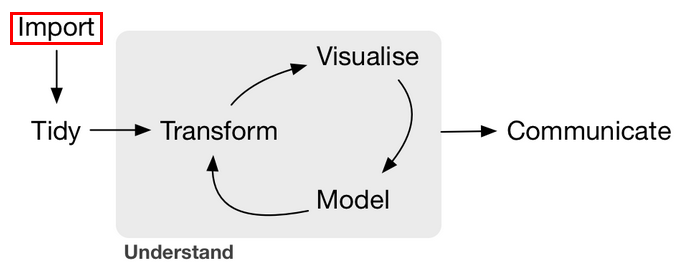
\includegraphics[width=0.75\textwidth]{../img/02_ciclo_1.png}
    \caption{Importación en el análisis de datos \textcite[Introducción]{grolemund2016r}.}
    \label{fig:ciclo1}
\end{figure}

Para aplicar las herramientas de R a nuestro trabajo, es necesario poder
importar nuestros datos a R. R tiene conectores ya implementados para
casi cualquier tipo y formato de datos. Entre los más comunes
están\footnote{La lista no pretende ser comprehensiva, sin embargo, se presentan algunos de los formatos de datos más comunes. De igual forma, se presentan algunas funciones que sirven para conectar \texttt{R} con datos que están guardados en un manejador de datos externo o en la nube. En caso de presentarse más de un método es porque aunque la recomendación de uso es la función en negritas, la otra opción es más antigua y muy utilizada.}:

\begin{longtable}[]{@{}lll@{}}
\toprule
Formato & Lectura & Escritura\tabularnewline
\midrule
\endhead
rds & \hyperref[rds]{base::readRDS} &
\hyperref[rds]{base::saveRDS}\tabularnewline
separado por * & \hyperref[separado-por]{utils::read.table};
\textbf{readr::read\_delim} &
\hyperref[separado-por]{utils::write.table};
\textbf{readr::write\_delim}\tabularnewline
csv & \hyperref[csv]{utils::read.csv}; \textbf{readr::read\_csv} &
\hyperref[csv]{utils::write.csv};
\textbf{readr::write\_csv}\tabularnewline
Microsoft Excel & \hyperref[microsoft-excel]{readxl::read\_excel} &
\hyperref[microsoft-excel]{xlsx::write.xlsx}\tabularnewline
dbf & \hyperref[dbf]{foreign::read.dbf} &
\hyperref[dbf]{foreign::write.dbf}\tabularnewline
IBM SPSS & \hyperref[ibm-spss]{haven::read\_sav} &
\hyperref[ibm-spss]{haven::write\_sav}\tabularnewline
Stata & \hyperref[stata]{haven::read\_dta} &
\hyperref[stata]{foreign::write.dta}\tabularnewline
SAS & \hyperref[sas]{haven::read\_sas} &
\hyperref[sas]{haven::write\_sas}\tabularnewline
Google spreadsheet &
\hyperref[google-spreadsheet]{googlesheets::gs\_read} &
\hyperref[google-spreadsheet]{googlesheets::gs\_new}\tabularnewline
Google bigquery & \hyperref[google-bigquery]{bigrquery::query\_exec}
&\tabularnewline
Heroku Postgres & \hyperref[heroku-postgres]{sql2df} &
\hyperref[heroku-postgres]{df2sql}\tabularnewline
rdata & \hyperref[rdata]{base::load} &
\hyperref[rdata]{base::save}\tabularnewline
\bottomrule
\end{longtable}

Los paquetes utilizados son (corre estos comandos en la consola):

\begin{Shaded}
\begin{Highlighting}[]
\KeywordTok{library}\NormalTok{(foreign)}
\KeywordTok{library}\NormalTok{(haven)}
\KeywordTok{library}\NormalTok{(readr)}
\KeywordTok{library}\NormalTok{(readxl)}
\KeywordTok{library}\NormalTok{(xlsx)}
\KeywordTok{library}\NormalTok{(googlesheets)}
\KeywordTok{library}\NormalTok{(bigrquery)}
\end{Highlighting}
\end{Shaded}

\begin{nota}[Importancia de rutas relativas]

Para leer un archivo, recordemos el comando \texttt{getwd()} para encontrar la carpeta
a la cual \texttt{R} esta dirigido en este momento. Una buena practica es considerar 
el directorio de trabajo como el lugar en donde esta guardado el archivo o \texttt{script} en el que se trabaja y ``moverse'' desde ahí hasta el archivo que se quiere leer.\\

Ya sea en escritura o en lectura, \texttt{R} buscará a partir del directorio
de trabajo (el que se despliega con \texttt{getwd()}) para buscar a partir 
de ahí el archivo por leer o para guardar el que se escribirá si se usan rutas
relativas.\\

En caso de usar rutas absolutas (a pesar de que esto \textbf{no} es una \textit{buena práctica}) se
hará lectura o escritura del archivo en el lugar especificado.
\end{nota}

\vspace{1cm}

\renewcommand\bcStyleTitre[1]{\large\textcolor{bbblack}{#1}}

\begin{bclogo}[
  couleur=llred,
  arrondi=0,
  logo=\bcstop,
  barre=none,
  noborder=true]{Ejercicios}
`R` tiene conexión con muchos de los formatos en los que se encuentran 
los datos. Veremos algunos de los mas relevantes.

El código en cada uno de los \texttt{chunks} (un chunk es el pedazo del documento
en donde hay código de \texttt{R}) está hecho para que puedas correrlo en la
consola (excepto cuando dice explícitamente \textit{do not run} (leyenda
comúnmente encontrada en los ejemplos de la documentación de las funciones. 
Con esto entenderás mejor el concepto de rutas relativas.
\end{bclogo}

\subsection{rds}\label{rds}

La extensión \texttt{rds} es de las más comúnmente utilizada en
\texttt{R}, por ejemplo, para guardar los datos para un paquete. Las
funciones pertenecen al \texttt{base} \parencite{rbase}. Permiten
guardar un solo objeto de \texttt{R} a un archivo y recuperarlo.

Para \textbf{escribirlos}

\begin{Shaded}
\begin{Highlighting}[]
\CommentTok{# Creamos un dataframe llamado misdatos}
\NormalTok{misdatos <-}\StringTok{ }\NormalTok{iris}
\CommentTok{# Los guardamos en comprimido}
\KeywordTok{saveRDS}\NormalTok{(misdatos, }\DataTypeTok{file =} \StringTok{"misdatos.rds"}\NormalTok{, }\DataTypeTok{ascii =} \OtherTok{FALSE}\NormalTok{, }\DataTypeTok{version =} \OtherTok{NULL}\NormalTok{,}
        \DataTypeTok{compress =} \OtherTok{TRUE}\NormalTok{, }\DataTypeTok{refhook =} \OtherTok{NULL}\NormalTok{)}
\end{Highlighting}
\end{Shaded}

Nota como si usas el comando \texttt{getwd()} y después vas a la ruta
indicada por medio del explorador de archivos, verás en esa carpeta el
archivo \texttt{misdatos.rds}.

Para \textbf{leerlos} usamos la ruta relativa. Dado que los guardamos en
el directorio de trabajo actual (Recuerda, se puede cambiar con el
comando \texttt{setwd}) entonces simplemente los llamamos:

\begin{Shaded}
\begin{Highlighting}[]
\NormalTok{misdatos <-}\StringTok{ }\KeywordTok{readRDS}\NormalTok{(}\StringTok{"misdatos.rds"}\NormalTok{)}
\CommentTok{# Los borramos}
\KeywordTok{file.remove}\NormalTok{(}\StringTok{"misdatos.rds"}\NormalTok{)}
\end{Highlighting}
\end{Shaded}

\subsection{separado por *}\label{separado-por}

Con esto nos referimos a la colección de archivos en texto plano, es
decir, \texttt{.txt}, \texttt{.tsv}, \texttt{.psv}, etcétera.

Para \textbf{escribirlos} el mas común es \texttt{write.table} del
paquete \texttt{utils} \parencite{utils}

\begin{Shaded}
\begin{Highlighting}[]
\CommentTok{# Do not run}
\KeywordTok{write.table}\NormalTok{(misdatos, }\DataTypeTok{file =} \StringTok{"~/misdatos.<extension>"}\NormalTok{, }\DataTypeTok{append =} \OtherTok{FALSE}
\NormalTok{, }\DataTypeTok{quote =} \OtherTok{TRUE}\NormalTok{, }\DataTypeTok{sep =} \StringTok{" "}\NormalTok{, }\DataTypeTok{eol =} \StringTok{"}\CharTok{\textbackslash{}n}\StringTok{"}\NormalTok{, }\DataTypeTok{na =} \StringTok{"NA"}\NormalTok{, }\DataTypeTok{dec =} \StringTok{"."}
\NormalTok{, }\DataTypeTok{row.names =} \OtherTok{TRUE}\NormalTok{, }\DataTypeTok{col.names =} \OtherTok{TRUE}
\NormalTok{, }\DataTypeTok{qmethod =} \KeywordTok{c}\NormalTok{(}\StringTok{"escape"}\NormalTok{, }\StringTok{"double"}\NormalTok{), }\DataTypeTok{fileEncoding =} \StringTok{""}\NormalTok{)}
\end{Highlighting}
\end{Shaded}

En el paquete \texttt{readr} se implementa también \texttt{write\_delim}

\begin{Shaded}
\begin{Highlighting}[]
\CommentTok{# Do not run}
\KeywordTok{write_delim}\NormalTok{(misdatos, }\DataTypeTok{path =} \StringTok{"~/misdatos.<extension>"}
\NormalTok{            , }\DataTypeTok{delim =} \StringTok{"}\CharTok{\textbackslash{}t}\StringTok{"}\NormalTok{, }\DataTypeTok{na =} \StringTok{"NA"}\NormalTok{, }\DataTypeTok{append =} \OtherTok{FALSE}\NormalTok{, }\DataTypeTok{col_names =} \OperatorTok{!}\NormalTok{append)}
\end{Highlighting}
\end{Shaded}

Escribamos ahora el \emph{dataframe} \texttt{misdatos} en \texttt{psv}:

\begin{Shaded}
\begin{Highlighting}[]
\KeywordTok{write_delim}\NormalTok{(misdatos, }\DataTypeTok{path =} \StringTok{"misdatos.psv"}\NormalTok{, }\DataTypeTok{delim =} \StringTok{"|"}\NormalTok{)}
\end{Highlighting}
\end{Shaded}

Para \textbf{leerlos} \texttt{read.table} del paquete \texttt{utils}
\parencite{utils} nos permite especificar casi cualquier particularidad
en un archivo de texto plano.

\begin{Shaded}
\begin{Highlighting}[]
\CommentTok{# Do not run}
\NormalTok{misdatos <-}\StringTok{ }\KeywordTok{read.table}\NormalTok{(}\StringTok{"~/misdatos.<extension>"}\NormalTok{, }\DataTypeTok{header =} \OtherTok{FALSE}
\NormalTok{                       , }\DataTypeTok{sep =} \StringTok{""}\NormalTok{, }\DataTypeTok{quote =} \StringTok{"}\CharTok{\textbackslash{}"}\StringTok{'"}\NormalTok{, }\DataTypeTok{dec =} \StringTok{"."}
\NormalTok{                       , }\DataTypeTok{numerals =} \KeywordTok{c}\NormalTok{(}\StringTok{"allow.loss"}\NormalTok{, }\StringTok{"warn.loss"}\NormalTok{, }\StringTok{"no.loss"}\NormalTok{)}
\NormalTok{                       , row.names, col.names, }\DataTypeTok{as.is =} \OperatorTok{!}\NormalTok{stringsAsFactors}
\NormalTok{                       , }\DataTypeTok{na.strings =} \StringTok{"NA"}\NormalTok{, }\DataTypeTok{colClasses =} \OtherTok{NA}\NormalTok{, }\DataTypeTok{nrows =} \OperatorTok{-}\DecValTok{1}
\NormalTok{                       , }\DataTypeTok{skip =} \DecValTok{0}\NormalTok{, }\DataTypeTok{check.names =} \OtherTok{TRUE}
\NormalTok{                       , }\DataTypeTok{fill =} \OperatorTok{!}\NormalTok{blank.lines.skip, }\DataTypeTok{strip.white =} \OtherTok{FALSE}
\NormalTok{                       , }\DataTypeTok{blank.lines.skip =} \OtherTok{TRUE}\NormalTok{, }\DataTypeTok{comment.char =} \StringTok{"#"}
\NormalTok{                       , }\DataTypeTok{allowEscapes =} \OtherTok{FALSE}\NormalTok{, }\DataTypeTok{flush =} \OtherTok{FALSE}
\NormalTok{                       , }\DataTypeTok{stringsAsFactors =} \KeywordTok{default.stringsAsFactors}\NormalTok{()}
\NormalTok{                       , }\DataTypeTok{fileEncoding =} \StringTok{""}\NormalTok{, }\DataTypeTok{encoding =} \StringTok{"unknown"}\NormalTok{, text}
\NormalTok{                       , }\DataTypeTok{skipNul =} \OtherTok{FALSE}\NormalTok{)}
\end{Highlighting}
\end{Shaded}

La función \texttt{read\_delim} del paquete \texttt{readr}
\parencite{readr} lee los datos más eficientemente a un objeto de clase
\texttt{tibble}.

\begin{Shaded}
\begin{Highlighting}[]
\CommentTok{# Do not run}
\NormalTok{misdatos <-}\StringTok{ }\KeywordTok{read_delim}\NormalTok{(}\DataTypeTok{file =} \StringTok{"~/misdatos.<extension>"}\NormalTok{, delim}
\NormalTok{                       , }\DataTypeTok{quote =} \StringTok{"}\CharTok{\textbackslash{}"}\StringTok{"}\NormalTok{, }\DataTypeTok{escape_backslash =} \OtherTok{FALSE}
\NormalTok{                       , }\DataTypeTok{escape_double =} \OtherTok{TRUE}\NormalTok{, }\DataTypeTok{col_names =} \OtherTok{TRUE}
\NormalTok{                       , }\DataTypeTok{col_types =} \OtherTok{NULL}\NormalTok{, }\DataTypeTok{locale =} \KeywordTok{default_locale}\NormalTok{()}
\NormalTok{                       , }\DataTypeTok{na =} \KeywordTok{c}\NormalTok{(}\StringTok{""}\NormalTok{, }\StringTok{"NA"}\NormalTok{), }\DataTypeTok{quoted_na =} \OtherTok{TRUE}\NormalTok{, }\DataTypeTok{comment =} \StringTok{""}
\NormalTok{                       , }\DataTypeTok{trim_ws =} \OtherTok{FALSE}\NormalTok{, }\DataTypeTok{skip =} \DecValTok{0}\NormalTok{, }\DataTypeTok{n_max =} \OtherTok{Inf}
\NormalTok{                       , }\DataTypeTok{guess_max =} \KeywordTok{min}\NormalTok{(}\DecValTok{1000}\NormalTok{, n_max)}
\NormalTok{                       , }\DataTypeTok{progress =} \KeywordTok{interactive}\NormalTok{())}
\end{Highlighting}
\end{Shaded}

Leemos el archivo \texttt{.psv} que creamos antes:

\begin{Shaded}
\begin{Highlighting}[]
\NormalTok{misdatos <-}\StringTok{ }\KeywordTok{read_delim}\NormalTok{(}\DataTypeTok{file =} \StringTok{"misdatos.psv"}\NormalTok{, }\DataTypeTok{delim =} \StringTok{"|"}\NormalTok{)}
\CommentTok{# Los borramos}
\KeywordTok{file.remove}\NormalTok{(}\StringTok{"misdatos.psv"}\NormalTok{)}
\end{Highlighting}
\end{Shaded}

\subsection{csv (archivo separado por
comas)}\label{csv-archivo-separado-por-comas}

Este es un caso particular de archivos de texto en el que se separan por
comas. Como es muy utilizado, generalmente se hacen funciones donde ya
se especifica el delimitador. Guardaremos el \emph{data frame}
\texttt{misdatos} en el directorio ``arriba'' de la ruta que se muestra
usando \texttt{getwd}. Esto lo podemos hacer anteponiendo al nombre del
archivo con \texttt{../}.

Para \textbf{escribirlos}

\begin{Shaded}
\begin{Highlighting}[]
\CommentTok{# utils }
\KeywordTok{write.csv}\NormalTok{(misdatos, }\DataTypeTok{file =} \StringTok{"../misdatos.csv"}\NormalTok{, }\DataTypeTok{row.names =}\NormalTok{ F)}
\CommentTok{# readr}
\KeywordTok{write_csv}\NormalTok{(misdatos, }\DataTypeTok{path =} \StringTok{"../misdatos.csv"}\NormalTok{, }\DataTypeTok{na =} \StringTok{"NA"}\NormalTok{, }\DataTypeTok{append =} \OtherTok{FALSE}\NormalTok{)}
\end{Highlighting}
\end{Shaded}

Observa en el explorador de archivos en dónde es que se guardó el
archivo \texttt{misdatos.csv}.

Para \textbf{leerlos}, seguimos usando rutas relativas.

\begin{Shaded}
\begin{Highlighting}[]
\CommentTok{# utils - como data.frame}
\NormalTok{misdatos <-}\StringTok{ }\KeywordTok{read.table}\NormalTok{(}\StringTok{"../misdatos.csv"}\NormalTok{, }\DataTypeTok{header=}\OtherTok{TRUE}\NormalTok{,}
   \DataTypeTok{sep=}\StringTok{","}\NormalTok{)}

\NormalTok{misdatos <-}\StringTok{ }\KeywordTok{read.csv}\NormalTok{(}\StringTok{"../misdatos.csv"}\NormalTok{)}

\CommentTok{# readr - como tibble}
\NormalTok{misdatos <-}\StringTok{ }\KeywordTok{read_csv}\NormalTok{(}\StringTok{"../misdatos.csv"}\NormalTok{)}

\CommentTok{# Lo borro}
\KeywordTok{file.remove}\NormalTok{(}\StringTok{"../misdatos.csv"}\NormalTok{)}
\end{Highlighting}
\end{Shaded}

\subsection{Microsoft Excel}\label{microsoft-excel}

Para \textbf{escribirlos} dentro del paquete \texttt{xlsx} usamos la
función \texttt{write.xlsx}

\begin{Shaded}
\begin{Highlighting}[]
\NormalTok{misdatos <-}\StringTok{ }\NormalTok{iris}
\KeywordTok{write.xlsx}\NormalTok{(misdatos, }\StringTok{"misdatos.xlsx"}\NormalTok{, }\DataTypeTok{row.names =}\NormalTok{ F)}
\end{Highlighting}
\end{Shaded}

Para \textbf{leerlos} dentro del paquete \texttt{readxl} se encuentra la
función \texttt{read\_excel} que es muy útil en este caso.

\begin{Shaded}
\begin{Highlighting}[]
\NormalTok{misdatos <-}\StringTok{ }\KeywordTok{read_excel}\NormalTok{(}\StringTok{"misdatos.xlsx"}\NormalTok{, }\DataTypeTok{sheet =} \DecValTok{1}\NormalTok{, }\DataTypeTok{col_names =} \OtherTok{TRUE}\NormalTok{, }
\DataTypeTok{col_types =} \OtherTok{NULL}\NormalTok{, }\DataTypeTok{na =} \StringTok{""}\NormalTok{, }\DataTypeTok{skip =} \DecValTok{0}\NormalTok{)}

\CommentTok{# Lo borro}
\KeywordTok{file.remove}\NormalTok{(}\StringTok{"misdatos.xlsx"}\NormalTok{)}
\end{Highlighting}
\end{Shaded}

\subsection{dbf}\label{dbf}

Extensión que representa un archivo de una base de datos (\emph{database
file}).

Para \textbf{escribirlos}:

\begin{Shaded}
\begin{Highlighting}[]
\KeywordTok{write.dbf}\NormalTok{(}\KeywordTok{as.data.frame}\NormalTok{(misdatos), }\StringTok{"misdatos.dbf"}\NormalTok{)}
\end{Highlighting}
\end{Shaded}

Nota cómo tuvimos que coercionar el objeto a \emph{data frame}. Como en
el ejemplo anterior leímos un \emph{tibble} y el paquete
\texttt{foreign} es más viejo (y no conoce los \emph{tibbles}) entonces
le mandamos un objeto que si conoce.

Veremos más adelante la ventaja de usar \emph{tibbles} aún cuando de vez
en cuando se tienen problemas de compatibilidad.

Para \textbf{leerlos}:

\begin{Shaded}
\begin{Highlighting}[]
\NormalTok{misdatos <-}\StringTok{ }\KeywordTok{read.dbf}\NormalTok{(}\StringTok{"misdatos.dbf"}\NormalTok{)}
\CommentTok{# Lo borro}
\KeywordTok{file.remove}\NormalTok{(}\StringTok{"misdatos.dbf"}\NormalTok{)}
\end{Highlighting}
\end{Shaded}

\subsection{IBM SPSS}\label{ibm-spss}

SPSS puede guardar los datos agregando etiquetas y otros metadatos. Para
evitar retrabajo, puede leerse directamente a \texttt{R}.

Para \textbf{escribirlos}

\begin{Shaded}
\begin{Highlighting}[]
\CommentTok{# haven}
\KeywordTok{write_sav}\NormalTok{(}\DataTypeTok{data =}\NormalTok{ misdatos, }\DataTypeTok{path =} \StringTok{"misdatos.sav"}\NormalTok{)}
\end{Highlighting}
\end{Shaded}

Para \textbf{leerlos}

\begin{Shaded}
\begin{Highlighting}[]
\CommentTok{# haven - como tibble}
\NormalTok{misdatos <-}\StringTok{ }\KeywordTok{read_sav}\NormalTok{(}\DataTypeTok{file =} \StringTok{"misdatos.sav"}\NormalTok{, }\DataTypeTok{user_na =} \OtherTok{FALSE}\NormalTok{)}

\CommentTok{# Lo borro}
\KeywordTok{file.remove}\NormalTok{(}\StringTok{"misdatos.sav"}\NormalTok{)}
\end{Highlighting}
\end{Shaded}

\subsection{Stata}\label{stata}

\begin{curiosidad}[HOME DIRECTORY]
El directorio (carpeta) \textit{home} es muy utilizado. Normalmente, se le 
denota como $\thicksim$ y es en donde un sistema operativo guarda los 
archivos del usuario que se encuentra en sesión. Dependiendo del sistema
operativo que utilices, encontrarás este directorio en una ruta específica.\\

En Microsoft Windows Vista 7, 8 y 10 lo encuentras en \texttt{<root>$\backslash$Users$\backslash$<username>}.\\

En Linux lo encuentras en \texttt{$/$home$/$<username>}.\\

En Mac OS X lo encuentras en \texttt{$/$Users$/$<username>}.
\end{curiosidad}

Para \textbf{escribirlos} en \texttt{Stata} primero tenemos que cambiar
los nombres de las variables en el \emph{data frame} pues \texttt{Stata}
no admite puntos en los nombres:

\begin{Shaded}
\begin{Highlighting}[]
\KeywordTok{names}\NormalTok{(misdatos) <-}\StringTok{ }\KeywordTok{tolower}\NormalTok{(}\KeywordTok{gsub}\NormalTok{(}\StringTok{"}\CharTok{\textbackslash{}\textbackslash{}}\StringTok{."}\NormalTok{, }\StringTok{"_"}\NormalTok{, }\KeywordTok{names}\NormalTok{(misdatos)))}
\CommentTok{# foreign}
\KeywordTok{write.dta}\NormalTok{(}\DataTypeTok{data =}\NormalTok{ misdatos, }\DataTypeTok{file =} \StringTok{"~/misdatos.dta"}\NormalTok{, }\DataTypeTok{version =} \DecValTok{12}\NormalTok{)}
\end{Highlighting}
\end{Shaded}

Para \textbf{leerlos}

\begin{Shaded}
\begin{Highlighting}[]
\CommentTok{# haven - como tibble}
\NormalTok{misdatos <-}\StringTok{ }\KeywordTok{read_dta}\NormalTok{(}\DataTypeTok{file =} \StringTok{"~/misdatos.dta"}\NormalTok{, }\DataTypeTok{encoding =} \OtherTok{NULL}\NormalTok{)}

\CommentTok{# Lo borramos}
\KeywordTok{file.remove}\NormalTok{(}\StringTok{"~/misdatos.dta"}\NormalTok{)}
\end{Highlighting}
\end{Shaded}

\subsection{SAS}\label{sas}

Para usar el paquete \texttt{haven} en este caso ejemplificaremos la
creación de un directorio de archivos en tu computadora desde
\texttt{R}:

\begin{Shaded}
\begin{Highlighting}[]
\CommentTok{# Creamos un directorio llamado datos}
\KeywordTok{dir.create}\NormalTok{(}\StringTok{"datos_sas"}\NormalTok{)}
\end{Highlighting}
\end{Shaded}

Observa como, en el directorio que se despliega con \texttt{getwd}
encuentras ahora una carpeta llamada \texttt{datos\_sas}. Creamos ahí un
archivo con la función \texttt{write\_sas} de \texttt{haven}. Nota que,
para \textbf{escribirlos}, también debemos asegurarnos que los nombres
de variables estén compuestos por letras, números o guiones bajos:

\begin{Shaded}
\begin{Highlighting}[]
\NormalTok{misdatos <-}\StringTok{ }\NormalTok{iris}
\KeywordTok{names}\NormalTok{(misdatos) <-}\StringTok{ }\KeywordTok{tolower}\NormalTok{(}\KeywordTok{gsub}\NormalTok{(}\StringTok{"}\CharTok{\textbackslash{}\textbackslash{}}\StringTok{."}\NormalTok{, }\StringTok{"_"}\NormalTok{, }\KeywordTok{names}\NormalTok{(misdatos)))}
\CommentTok{# haven}
\KeywordTok{write_sas}\NormalTok{(}\DataTypeTok{data =}\NormalTok{ misdatos, }\DataTypeTok{path =} \StringTok{"datos_sas/misdatos.sas7bdat"}\NormalTok{)}
\end{Highlighting}
\end{Shaded}

Para leerlos, utilizamos \texttt{read\_sas} del paquete \texttt{haven}:

\begin{Shaded}
\begin{Highlighting}[]
\CommentTok{# haven - como tibble}
\NormalTok{misdatos <-}\StringTok{ }\KeywordTok{read_sas}\NormalTok{(}\StringTok{"datos_sas/misdatos.sas7bdat"}
\NormalTok{                     , }\DataTypeTok{catalog_file =} \OtherTok{NULL}\NormalTok{, }\DataTypeTok{encoding =} \OtherTok{NULL}\NormalTok{)}
\end{Highlighting}
\end{Shaded}

Observa desde el explorador de archivos, cómo se creó el archivo dentro
del directorio \texttt{datos\_sas/}. También desde \texttt{R} podemos
borrar el directorio:

\begin{Shaded}
\begin{Highlighting}[]
\KeywordTok{unlink}\NormalTok{(}\StringTok{"datos_sas"}\NormalTok{, }\DataTypeTok{recursive =}\NormalTok{ T, }\DataTypeTok{force =} \OtherTok{FALSE}\NormalTok{)}
\end{Highlighting}
\end{Shaded}

La bandera \texttt{recursive} le dice al sistema que borre todo lo
contenido en esa carpeta.

\subsection{Google Spreadsheet}\label{google-spreadsheet}

Para hacer este ejercicio, debes tener una cuenta de \texttt{gmail}.

Primero, debe realizarse la autenticación. Esto lo puedes hacer en
cualquier sesión interactiva utilizando alguna función del paquete
\texttt{googlesheets}

\begin{Shaded}
\begin{Highlighting}[]
\KeywordTok{gs_ls}\NormalTok{()}
\end{Highlighting}
\end{Shaded}

En la consola de \texttt{R} te aparece:

\begin{figure}[H]
\centering
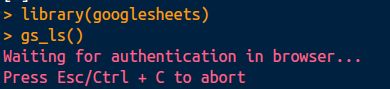
\includegraphics[width=0.3\textwidth]{../img/gs_oauth1.png}
\end{figure}

Se abrirá una ventana del explorador y deberás introducir tus
credenciales de tu cuenta de \texttt{gmail}

\begin{figure}[H]
\centering
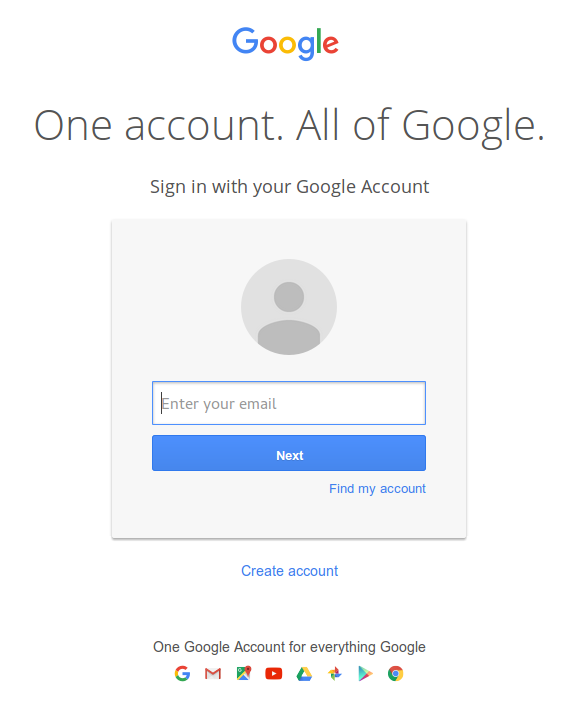
\includegraphics[width=0.5\textwidth]{../img/gs_oauth2.png}
\end{figure}

Después de poner tus credenciales, te aparecerá un mensaje pidiendo
acceso a tus datos en \texttt{drive}:

\begin{figure}[H]
\centering
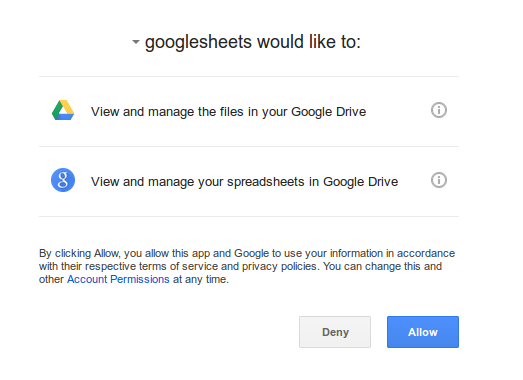
\includegraphics[width=0.5\textwidth]{../img/gs_oauth3.png}
\end{figure}

Al aceptar darle acceso, recibirás un mensaje parecido a
\emph{Authentication complete. Please close this page and return to R.}

Ahora verás en la consola de R un listado de las
\texttt{google\ spreadsheets} en tu cuenta de \texttt{gmail}.

Ahora, vamos a \textbf{escribir} una nueva hoja en tu cuenta.

\begin{Shaded}
\begin{Highlighting}[]
\KeywordTok{gs_new}\NormalTok{(}\StringTok{"misdatos"}\NormalTok{, }\DataTypeTok{ws_title =} \StringTok{"mihoja"}\NormalTok{, }\DataTypeTok{input =} \KeywordTok{head}\NormalTok{(iris)}
\NormalTok{       , }\DataTypeTok{trim =} \OtherTok{TRUE}\NormalTok{, }\DataTypeTok{verbose =} \OtherTok{FALSE}\NormalTok{)}
\end{Highlighting}
\end{Shaded}

Si vas a tu google drive, deberás ver que se creó un nuevo elemento que
se ve así:

\begin{figure}[H]
\centering
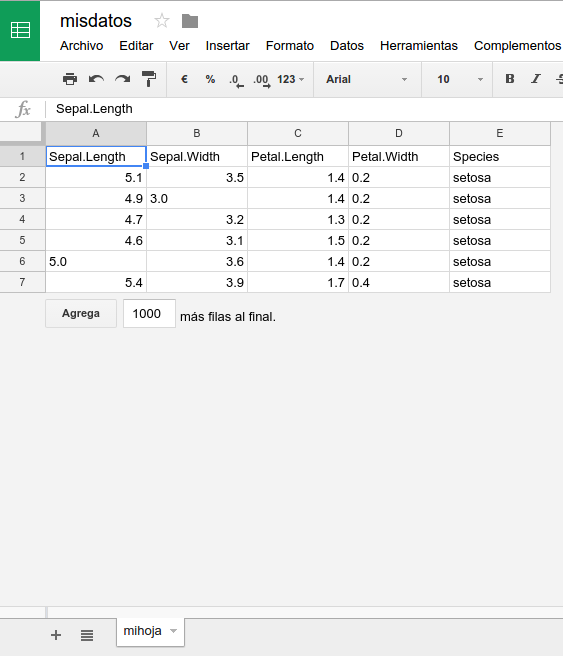
\includegraphics[width=0.5\textwidth]{../img/gs_nuevo.png}
\end{figure}

De igual forma, puedes ahora \textbf{leer} los datos de cualquier
\texttt{google\ spreadsheet} que tengas en tu cuenta.

\begin{Shaded}
\begin{Highlighting}[]
\NormalTok{misdatos <-}\StringTok{ }\KeywordTok{gs_read}\NormalTok{(}\KeywordTok{gs_title}\NormalTok{(}\StringTok{"misdatos"}\NormalTok{), }\DataTypeTok{ws =} \StringTok{"mihoja"}\NormalTok{)}
\CommentTok{# La borro}
\KeywordTok{gs_delete}\NormalTok{(}\KeywordTok{gs_title}\NormalTok{(}\StringTok{"misdatos"}\NormalTok{))}
\end{Highlighting}
\end{Shaded}

\subsection{Google bigquery}\label{google-bigquery}

\texttt{Google\ bigquery} es un \emph{data warehouse} que permite
guardar grandes bases de datos. Al contratar el servicio,
\texttt{google} se encarga del \emph{hardware} y la infraestructura
necesaria para que su procesamiento sea rápido
\parencite{whatisbigquery}.

Para guardar tus datos en \texttt{bigquery} debes crear un proyecto en
\href{https://console.developers.google.com/apis/library}{la consola de
desarrolladores}.

Existen varias bases de dato públicas disponibles. Para poder
utilizarlas, necesitas tener una cuenta. Puedes empezar una prueba
gratis en \href{https://cloud.google.com/free-trial/}{la página de
google cloud platform.} Verás una pantalla como esta:

\begin{figure}[H]
\centering
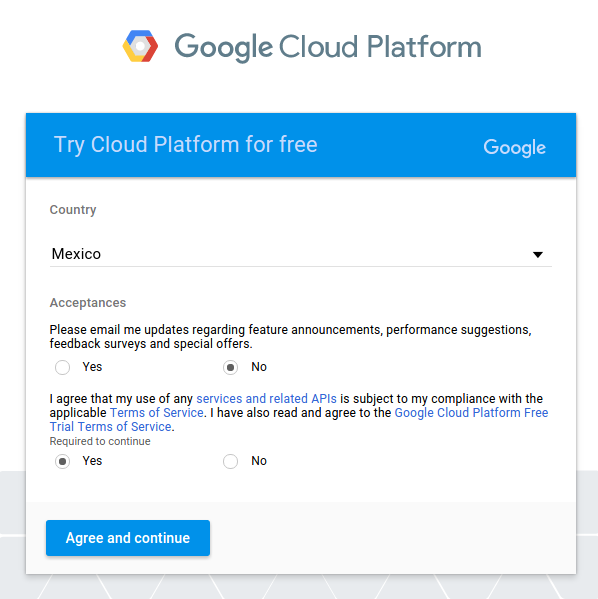
\includegraphics[width=0.5\textwidth]{../img/bq1.png}
\end{figure}

Sigue las instrucciones y eventualmente llegarás a una pantalla como
esta

\begin{figure}[H]
\centering
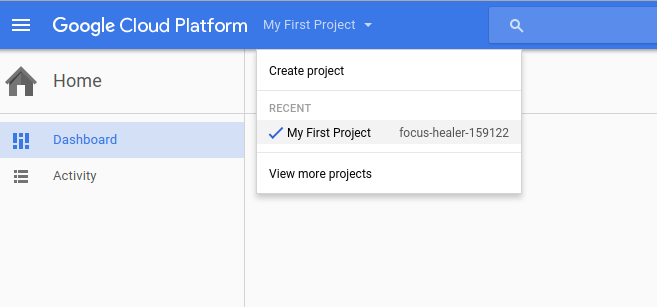
\includegraphics[width=0.5\textwidth]{../img/bq2.png}
\end{figure}

Copia el identificador de tu proyecto para que puedas realizar
\texttt{queries} (llamadas a las bases de datos).

Leemos la base de datos pública de natalidad en Estados Unidos.

\begin{Shaded}
\begin{Highlighting}[]
\NormalTok{project <-}\StringTok{ "focus-healer-159122"} \CommentTok{# pon tu projectID aquí}
 
\NormalTok{sql <-}\StringTok{ 'SELECT year, count(*) as babies, avg(mother_age) as mother_age_avg}
\StringTok{FROM[publicdata:samples.natality] }
\StringTok{WHERE year > 1980 and year < 2006}
\StringTok{group by year;'}
 
\NormalTok{data <-}\StringTok{ }\KeywordTok{query_exec}\NormalTok{(}\DataTypeTok{query =}\NormalTok{ sql, }\DataTypeTok{project =}\NormalTok{ project)}
\end{Highlighting}
\end{Shaded}

Nota como la tabla cuenta con aproximadamente. 140 millones de registros
y se obtiene el detalle en segundos.

\subsection{Heroku Postgres}\label{heroku-postgres}

\texttt{R} no es un manejador de base de datos y, por ende, no es un
lenguaje que permite trabajar con una gran cantidad de datos. \texttt{R}
guarda los objetos utilizando la memoria virtual de la computadora,
i.e.~la RAM, misma que depende de varios elementos (incluido el sistema
operativo) y que limita los datos que podrán ser procesados.

Cuando necesitamos conocer el tamaño de los datos que están en el
ambiente de trabajo, puede utilizarse el paquete \texttt{pryr}
\parencite[][sección ``the role of physical memory'']{pryr}.

\begin{Shaded}
\begin{Highlighting}[]
\KeywordTok{rm}\NormalTok{(}\DataTypeTok{list =} \KeywordTok{ls}\NormalTok{()) }\CommentTok{# borramos los objetos del ambiente}
\CommentTok{# Cargamos datos al ambiente}
\NormalTok{flights <-}\StringTok{ }\KeywordTok{read_csv}\NormalTok{(}\StringTok{"data/flights.csv"}\NormalTok{)}
\NormalTok{airports <-}\StringTok{ }\KeywordTok{read_csv}\NormalTok{(}\StringTok{"data/airports.csv"}\NormalTok{)}
\NormalTok{planes <-}\StringTok{ }\KeywordTok{read_csv}\NormalTok{(}\StringTok{"data/planes.csv"}\NormalTok{)}
\KeywordTok{ls}\NormalTok{() }\CommentTok{# mostramos los objetos en el ambiente}

\KeywordTok{library}\NormalTok{(pryr) }\CommentTok{# Cargamos el paquete pryr}
\KeywordTok{mem_used}\NormalTok{() }\CommentTok{# memoria utilizada}

\KeywordTok{object_size}\NormalTok{(flights, }\DataTypeTok{units =} \StringTok{"Mb"}\NormalTok{) }\CommentTok{# Obtenemos el tamaño de un objeto}
\KeywordTok{sapply}\NormalTok{(}\KeywordTok{ls}\NormalTok{(), }\ControlFlowTok{function}\NormalTok{(x) }\KeywordTok{object_size}\NormalTok{(}\KeywordTok{get}\NormalTok{(x))) }\CommentTok{# de todos en el ambiente}
\end{Highlighting}
\end{Shaded}

Las estrategias en memoria se revisaron brevemente en el apartado XXX,
en este caso, es pertinente mencionar las estrategias fuera de memoria
(\emph{out of memory}).

Es posible explorar un conjunto de datos sin necesidad de cargarlos en
\texttt{R} pero utilizando comandos de \texttt{R} y trabajando desde un
script de \texttt{R}, permitiendo que herramientas más eficientes (y
apropiadas) para el trabajo de grandes volúmenes de datos realicen el
procesamiento de los mismos.

Los sistemas gestores de base de datos están optimizados para almacenar
y buscar en grandes volúmenes de datos en forma más eficiente que
\texttt{R}. Algunos ejemplos populares son Oracle y PostgreSQL
\parencite[][sección ``working with large datasets'']{peng2016m}. Hay
múltiples paquetes que permiten establecer una conexión con estos
sistemas desde una sesión de \texttt{R}.

Los paquetes \texttt{DBI} y \texttt{Postgresql} permiten realizar esta
tarea. Debido a que requieren credenciales se muestra una función para
leer datos desde \texttt{PostgreSQL} y escribirlos sin necesidad de
poner las credenciales dentro del mismo script.

Para que funcionen apropiadamente, es necesario poner en el directorio
de trabajo un archivo llamado \texttt{parametros.yaml} en donde se
escriben las credenciales para Postgres:

\begin{verbatim}
host : localhost
db : postgres
username : usr
password : password
\end{verbatim}

Nota: el salto de línea en la última línea es importante.

Para leer datos, creamos una función a la que podemos enviarle una
cadena de comandos en SQL.

\begin{Shaded}
\begin{Highlighting}[]
\NormalTok{sql2df <-}\StringTok{ }\ControlFlowTok{function}\NormalTok{(sql.file, }\DataTypeTok{df.file =} \StringTok{""}\NormalTok{) \{}
  \KeywordTok{require}\NormalTok{(DBI)}
  \KeywordTok{require}\NormalTok{(futile.logger)}
  \KeywordTok{require}\NormalTok{(yaml)}
  \KeywordTok{require}\NormalTok{(RPostgreSQL)}
  
  \ControlFlowTok{if}\NormalTok{(}\OperatorTok{!}\KeywordTok{file.exists}\NormalTok{(df.file)) \{}
    \ControlFlowTok{if}\NormalTok{(}\KeywordTok{file.exists}\NormalTok{(}\StringTok{"./parametros.yaml"}\NormalTok{)) \{}
\NormalTok{      x <-}\StringTok{ }\NormalTok{yaml}\OperatorTok{::}\KeywordTok{yaml.load_file}\NormalTok{(}\StringTok{"./parametros.yaml"}\NormalTok{)}
\NormalTok{    \} }\ControlFlowTok{else}\NormalTok{ \{}
\NormalTok{      x <-}\StringTok{ }\NormalTok{yaml}\OperatorTok{::}\KeywordTok{yaml.load_file}\NormalTok{(}\StringTok{"../parametros.yaml"}\NormalTok{)}
\NormalTok{    \}}
    
    \CommentTok{# Creamos la conexión a la base de datos}
\NormalTok{    futile.logger}\OperatorTok{::}\KeywordTok{flog.info}\NormalTok{(}\StringTok{"Conectando a la base de datos"}\NormalTok{)}
    
\NormalTok{    con <-}\StringTok{ }\KeywordTok{dbConnect}\NormalTok{(RPostgreSQL}\OperatorTok{::}\KeywordTok{PostgreSQL}\NormalTok{(), }\DataTypeTok{dbname =}\NormalTok{ x}\OperatorTok{$}\NormalTok{db, }
                     \DataTypeTok{host =}\NormalTok{ x}\OperatorTok{$}\NormalTok{host, }
                     \DataTypeTok{port =} \DecValTok{5432}\NormalTok{, }
                     \DataTypeTok{user =}\NormalTok{ x}\OperatorTok{$}\NormalTok{username,}
                     \DataTypeTok{password =}\NormalTok{ x}\OperatorTok{$}\NormalTok{password)}
    
\NormalTok{    futile.logger}\OperatorTok{::}\KeywordTok{flog.info}\NormalTok{(}\StringTok{"Conectado a %s, como %s"}\NormalTok{, x}\OperatorTok{$}\NormalTok{host, x}\OperatorTok{$}\NormalTok{username)}
    
    \CommentTok{# Leemos el query}
\NormalTok{    sql <-}\StringTok{ }\KeywordTok{paste}\NormalTok{(}\KeywordTok{readLines}\NormalTok{(sql.file,}\DataTypeTok{encoding=}\StringTok{"UTF-8"}\NormalTok{)}
\NormalTok{                 , }\DataTypeTok{sep=}\StringTok{" "}\NormalTok{, }\DataTypeTok{collapse=}\StringTok{" "}\NormalTok{)}
    
    \KeywordTok{tryCatch}\NormalTok{( \{}
\NormalTok{      futile.logger}\OperatorTok{::}\KeywordTok{flog.info}\NormalTok{(}\StringTok{"Ejecutando el query"}\NormalTok{)}
      \CommentTok{# Creamos el query}
\NormalTok{      rs <-}\StringTok{ }\NormalTok{RPostgreSQL}\OperatorTok{::}\KeywordTok{dbSendQuery}\NormalTok{(con, sql)}
\NormalTok{      futile.logger}\OperatorTok{::}\KeywordTok{flog.info}\NormalTok{(}\StringTok{"Obteniendo los datos"}\NormalTok{)}
      \CommentTok{# Obtenemos los datos}
\NormalTok{      df <-}\StringTok{ }\NormalTok{DBI}\OperatorTok{::}\KeywordTok{dbFetch}\NormalTok{(rs)}
      \CommentTok{# Liberamos el ResultSet}
\NormalTok{      futile.logger}\OperatorTok{::}\KeywordTok{flog.info}\NormalTok{(}\StringTok{"Limpiando el result set"}\NormalTok{)}
\NormalTok{      RPostgreSQL}\OperatorTok{::}\KeywordTok{dbClearResult}\NormalTok{(rs)}
\NormalTok{    \}, }\DataTypeTok{finally=}\NormalTok{RPostgreSQL}\OperatorTok{::}\KeywordTok{dbDisconnect}\NormalTok{(con) }\CommentTok{# Nos desconectamos de la BD}
\NormalTok{    )}
    
    \ControlFlowTok{if}\NormalTok{(df.file }\OperatorTok{!=}\StringTok{ ""}\NormalTok{)\{ }
      \KeywordTok{saveRDS}\NormalTok{(}\DataTypeTok{object=}\NormalTok{df, }\DataTypeTok{file=}\NormalTok{df.file)  }
\NormalTok{    \}}
\NormalTok{  \} }\ControlFlowTok{else}\NormalTok{ \{}
\NormalTok{    df <-}\StringTok{ }\KeywordTok{readRDS}\NormalTok{(df.file)}
\NormalTok{  \}}
  
  \KeywordTok{return}\NormalTok{(df)}
\NormalTok{\}}
\end{Highlighting}
\end{Shaded}

La función
\texttt{sql2df}\footnote{Función adaptada de notas de Adolfo de Únanue.}
recibe como parámetro, como cadena, la ruta hacia un archivo de
extensión \texttt{.sql} con los comandos a ejecutar en el manejador de
base de datos. Éste puede verse, por ejemplo, como:

\begin{verbatim}
select * 
from information_schema.tables 
where table_schema = 'information_schema';
\end{verbatim}

Guardamos ésta en el archivo \texttt{sql/ejemplo.sql} la cláusula de
arriba. Después, llamamos a la función.

\begin{Shaded}
\begin{Highlighting}[]
\NormalTok{datos <-}\StringTok{ }\KeywordTok{sql2df}\NormalTok{(}\StringTok{"sql/ejemplo.sql"}\NormalTok{, }\DataTypeTok{df.file =} \StringTok{"ejemplo.rds"}\NormalTok{)}
\KeywordTok{head}\NormalTok{(datos)}
\end{Highlighting}
\end{Shaded}

Con el parámetro \texttt{df.file} es posible especificar una ruta para
que se guarde una copia local del resultado de los datos. Esto es útil
cuando se está trabajando con los datos, de forma que sea más rápido el
trabajo con los mismos.

Para escribir datos, podemos utilizar la función siguiente:

\begin{Shaded}
\begin{Highlighting}[]
\NormalTok{df2sql <-}\StringTok{ }\ControlFlowTok{function}\NormalTok{(data.frame, df.schema.name, df.table.name, }\DataTypeTok{owner.to =} \OtherTok{NA}\NormalTok{) \{}
  \KeywordTok{require}\NormalTok{(DBI)}
  \KeywordTok{require}\NormalTok{(futile.logger)}
  \KeywordTok{require}\NormalTok{(yaml)}
  \KeywordTok{require}\NormalTok{(RPostgreSQL)}
\NormalTok{  data.frame <-}\StringTok{ }\KeywordTok{data.frame}\NormalTok{(data.frame)}
  \CommentTok{# Normalizamos nombres}
  \KeywordTok{names}\NormalTok{(data.frame) <-}\StringTok{ }\KeywordTok{normalizarNombres}\NormalTok{(}\KeywordTok{names}\NormalTok{(data.frame))}
  
  \ControlFlowTok{if}\NormalTok{(}\KeywordTok{file.exists}\NormalTok{(}\StringTok{"./parametros.yaml"}\NormalTok{)) \{}
\NormalTok{    x <-}\StringTok{ }\NormalTok{yaml}\OperatorTok{::}\KeywordTok{yaml.load_file}\NormalTok{(}\StringTok{"./parametros.yaml"}\NormalTok{)}
\NormalTok{  \} }\ControlFlowTok{else}\NormalTok{ \{}
\NormalTok{    x <-}\StringTok{ }\NormalTok{yaml}\OperatorTok{::}\KeywordTok{yaml.load_file}\NormalTok{(}\StringTok{"../parametros.yaml"}\NormalTok{)}
\NormalTok{  \}}
   
  \CommentTok{# Creamos la conexión a la base de datos}
\NormalTok{  futile.logger}\OperatorTok{::}\KeywordTok{flog.info}\NormalTok{(}\StringTok{"Conectando a la base de datos"}\NormalTok{)}
    
\NormalTok{  con <-}\StringTok{ }\KeywordTok{dbConnect}\NormalTok{(RPostgreSQL}\OperatorTok{::}\KeywordTok{PostgreSQL}\NormalTok{(), }\DataTypeTok{dbname =}\NormalTok{ x}\OperatorTok{$}\NormalTok{db, }
                     \DataTypeTok{host =}\NormalTok{ x}\OperatorTok{$}\NormalTok{host, }
                     \DataTypeTok{port =} \DecValTok{5432}\NormalTok{, }
                     \DataTypeTok{user =}\NormalTok{ x}\OperatorTok{$}\NormalTok{username,}
                     \DataTypeTok{password =}\NormalTok{ x}\OperatorTok{$}\NormalTok{password)}
\NormalTok{  futile.logger}\OperatorTok{::}\KeywordTok{flog.info}\NormalTok{(}\StringTok{"Conectado a %s, como %s"}
\NormalTok{                           , x}\OperatorTok{$}\NormalTok{host, x}\OperatorTok{$}\NormalTok{username)}
  
  \KeywordTok{tryCatch}\NormalTok{( \{}
    \KeywordTok{flog.info}\NormalTok{(}\StringTok{"Ejecutando la escritura de tabla %s en el esquema %s"}
\NormalTok{              , df.table.name, df.schema.name)}
    \CommentTok{# Definimos el camino al esquema deseado}
    \ControlFlowTok{if}\NormalTok{(df.schema.name }\OperatorTok{!=}\StringTok{ "public"}\NormalTok{)\{}
      \KeywordTok{dbSendQuery}\NormalTok{(}\DataTypeTok{conn =}\NormalTok{ con}
\NormalTok{                  , }\DataTypeTok{statement =} \KeywordTok{paste0}\NormalTok{(}\StringTok{"SET search_path = "}
\NormalTok{                                       , df.schema.name, }\StringTok{", public;"}\NormalTok{))}
\NormalTok{    \}}
\NormalTok{    long.name <-}\StringTok{ }\KeywordTok{paste0}\NormalTok{(df.schema.name, }\StringTok{"."}\NormalTok{, df.table.name)}
    \CommentTok{# Escribimos la tabla}
    \KeywordTok{dbWriteTable}\NormalTok{(con,}
\NormalTok{                 df.table.name,}
\NormalTok{                 data.frame,}
                 \DataTypeTok{overwrite=}\OtherTok{FALSE}\NormalTok{,}
                 \DataTypeTok{append =} \OtherTok{TRUE}\NormalTok{)}
    
    \KeywordTok{flog.info}\NormalTok{(}\StringTok{"Escribiendo los datos"}\NormalTok{)}
    
    \ControlFlowTok{if}\NormalTok{(}\OperatorTok{!}\KeywordTok{is.na}\NormalTok{(owner.to))\{}
      \KeywordTok{flog.info}\NormalTok{(}\StringTok{"Otorgando ownership a %s"}\NormalTok{, owner.to)}
      \KeywordTok{dbSendQuery}\NormalTok{(con, }\KeywordTok{paste0}\NormalTok{(}\StringTok{"alter table "}\NormalTok{, long.name}
\NormalTok{                              , }\StringTok{" owner to "}\NormalTok{, owner.to, }\StringTok{";"}\NormalTok{))}
\NormalTok{    \}}
    
\NormalTok{  \}, }\DataTypeTok{finally=}\KeywordTok{dbDisconnect}\NormalTok{(con) }\CommentTok{# Nos desconectamos de la BD}
\NormalTok{  )}
  \KeywordTok{flog.info}\NormalTok{(}\StringTok{"Escritura finalizada"}\NormalTok{)}
\NormalTok{\}}

\CommentTok{# Función de ayuda}
\NormalTok{normalizarNombres <-}\StringTok{ }\ControlFlowTok{function}\NormalTok{(column_names) \{}
  \KeywordTok{require}\NormalTok{(magrittr)}
  \KeywordTok{gsub}\NormalTok{(}\StringTok{"}\CharTok{\textbackslash{}\textbackslash{}}\StringTok{s+"}\NormalTok{, }\StringTok{" "}\NormalTok{, stringr}\OperatorTok{::}\KeywordTok{str_trim}\NormalTok{(column_names)) }\OperatorTok
\StringTok{    }\KeywordTok{gsub}\NormalTok{(}\StringTok{"^ *|(?<= ) | *$"}\NormalTok{, }\StringTok{""}\NormalTok{, ., }\DataTypeTok{perl=}\NormalTok{T) }\OperatorTok
\StringTok{    }\KeywordTok{gsub}\NormalTok{(}\StringTok{'}\CharTok{\textbackslash{}\textbackslash{}}\StringTok{ |}\CharTok{\textbackslash{}\textbackslash{}}\StringTok{.'}\NormalTok{, }\StringTok{'_'}\NormalTok{, .) }\OperatorTok
\StringTok{    }\KeywordTok{gsub}\NormalTok{(}\StringTok{"([a-z])([A-Z])"}\NormalTok{, }\StringTok{"}\CharTok{\textbackslash{}\textbackslash{}}\StringTok{1_}\CharTok{\textbackslash{}\textbackslash{}}\StringTok{L}\CharTok{\textbackslash{}\textbackslash{}}\StringTok{2"}\NormalTok{, ., }\DataTypeTok{perl =} \OtherTok{TRUE}\NormalTok{) }\OperatorTok
\StringTok{    }\KeywordTok{gsub}\NormalTok{(}\StringTok{'ñ'}\NormalTok{, }\StringTok{'n'}\NormalTok{, .) }\OperatorTok
\StringTok{    }\KeywordTok{iconv}\NormalTok{(., }\DataTypeTok{to=}\StringTok{'ASCII//TRANSLIT'}\NormalTok{) }\OperatorTok
\StringTok{    }\KeywordTok{tolower}\NormalTok{(.)}
\NormalTok{\}}
\end{Highlighting}
\end{Shaded}

Se especifican en los parámetros el data.frame a escribir, una cadena de
caracteres indicando el esquema en el que se escribirá la base, una
cadena indicando el nombre de la tabla y es posible especificar qué
dueño deberá asignarse para la base:

\begin{Shaded}
\begin{Highlighting}[]
\KeywordTok{df2sql}\NormalTok{(iris, }\StringTok{"public"}\NormalTok{, }\StringTok{"iris"}\NormalTok{, }\DataTypeTok{owner.to =} \StringTok{"usr"}\NormalTok{)}
\end{Highlighting}
\end{Shaded}

\subsection{rdata}\label{rdata}

También es posible guardar objetos específicos del ambiente dentro de un
formato especial con extensión \texttt{rdata} o \texttt{RData}. Esto es
muy útil, por ejemplo, para guardar modelos u otros objetos y después
poder utilizarlos en producción o en alguna aplicación que requiera un
tiempo de respuesta bajo.

Para \textbf{escribirlos}

\begin{Shaded}
\begin{Highlighting}[]
\KeywordTok{save}\NormalTok{(..., }
     \DataTypeTok{file =} \StringTok{"~/misdatos.rdata"}\NormalTok{,}
     \DataTypeTok{ascii =} \OtherTok{FALSE}\NormalTok{, }\DataTypeTok{version =} \OtherTok{NULL}\NormalTok{, }\DataTypeTok{envir =} \KeywordTok{parent.frame}\NormalTok{(),}
     \DataTypeTok{compress =} \KeywordTok{isTRUE}\NormalTok{(}\OperatorTok{!}\NormalTok{ascii), compression_level,}
     \DataTypeTok{eval.promises =} \OtherTok{TRUE}\NormalTok{, }\DataTypeTok{precheck =} \OtherTok{TRUE}\NormalTok{)}
\end{Highlighting}
\end{Shaded}

Nota como \texttt{...} pueden ser uno o más objetos de \texttt{R}.

Para \textbf{leerlos}

\begin{Shaded}
\begin{Highlighting}[]
\KeywordTok{load}\NormalTok{(}\StringTok{"~/misdatos.rdata"}\NormalTok{)}
\end{Highlighting}
\end{Shaded}

Los objetos se cargarán al ambiente con los nombres con los que fueron
guardados.


\end{document}

\documentclass[]{article}
\usepackage{lmodern}
\usepackage{amssymb,amsmath}
\usepackage{ifxetex,ifluatex}
\usepackage{fixltx2e} % provides \textsubscript
\ifnum 0\ifxetex 1\fi\ifluatex 1\fi=0 % if pdftex
  \usepackage[T1]{fontenc}
  \usepackage[utf8]{inputenc}
\else % if luatex or xelatex
  \ifxetex
    \usepackage{mathspec}
  \else
    \usepackage{fontspec}
  \fi
  \defaultfontfeatures{Ligatures=TeX,Scale=MatchLowercase}
\fi
% use upquote if available, for straight quotes in verbatim environments
\IfFileExists{upquote.sty}{\usepackage{upquote}}{}
% use microtype if available
\IfFileExists{microtype.sty}{%
\usepackage{microtype}
\UseMicrotypeSet[protrusion]{basicmath} % disable protrusion for tt fonts
}{}
\usepackage[margin=1in]{geometry}
\usepackage{hyperref}
\hypersetup{unicode=true,
            pdftitle={R: Transformación de datos},
            pdfborder={0 0 0},
            breaklinks=true}
\urlstyle{same}  % don't use monospace font for urls
\usepackage{color}
\usepackage{fancyvrb}
\newcommand{\VerbBar}{|}
\newcommand{\VERB}{\Verb[commandchars=\\\{\}]}
\DefineVerbatimEnvironment{Highlighting}{Verbatim}{commandchars=\\\{\}}
% Add ',fontsize=\small' for more characters per line
\usepackage{framed}
\definecolor{shadecolor}{RGB}{248,248,248}
\newenvironment{Shaded}{\begin{snugshade}}{\end{snugshade}}
\newcommand{\KeywordTok}[1]{\textcolor[rgb]{0.13,0.29,0.53}{\textbf{#1}}}
\newcommand{\DataTypeTok}[1]{\textcolor[rgb]{0.13,0.29,0.53}{#1}}
\newcommand{\DecValTok}[1]{\textcolor[rgb]{0.00,0.00,0.81}{#1}}
\newcommand{\BaseNTok}[1]{\textcolor[rgb]{0.00,0.00,0.81}{#1}}
\newcommand{\FloatTok}[1]{\textcolor[rgb]{0.00,0.00,0.81}{#1}}
\newcommand{\ConstantTok}[1]{\textcolor[rgb]{0.00,0.00,0.00}{#1}}
\newcommand{\CharTok}[1]{\textcolor[rgb]{0.31,0.60,0.02}{#1}}
\newcommand{\SpecialCharTok}[1]{\textcolor[rgb]{0.00,0.00,0.00}{#1}}
\newcommand{\StringTok}[1]{\textcolor[rgb]{0.31,0.60,0.02}{#1}}
\newcommand{\VerbatimStringTok}[1]{\textcolor[rgb]{0.31,0.60,0.02}{#1}}
\newcommand{\SpecialStringTok}[1]{\textcolor[rgb]{0.31,0.60,0.02}{#1}}
\newcommand{\ImportTok}[1]{#1}
\newcommand{\CommentTok}[1]{\textcolor[rgb]{0.56,0.35,0.01}{\textit{#1}}}
\newcommand{\DocumentationTok}[1]{\textcolor[rgb]{0.56,0.35,0.01}{\textbf{\textit{#1}}}}
\newcommand{\AnnotationTok}[1]{\textcolor[rgb]{0.56,0.35,0.01}{\textbf{\textit{#1}}}}
\newcommand{\CommentVarTok}[1]{\textcolor[rgb]{0.56,0.35,0.01}{\textbf{\textit{#1}}}}
\newcommand{\OtherTok}[1]{\textcolor[rgb]{0.56,0.35,0.01}{#1}}
\newcommand{\FunctionTok}[1]{\textcolor[rgb]{0.00,0.00,0.00}{#1}}
\newcommand{\VariableTok}[1]{\textcolor[rgb]{0.00,0.00,0.00}{#1}}
\newcommand{\ControlFlowTok}[1]{\textcolor[rgb]{0.13,0.29,0.53}{\textbf{#1}}}
\newcommand{\OperatorTok}[1]{\textcolor[rgb]{0.81,0.36,0.00}{\textbf{#1}}}
\newcommand{\BuiltInTok}[1]{#1}
\newcommand{\ExtensionTok}[1]{#1}
\newcommand{\PreprocessorTok}[1]{\textcolor[rgb]{0.56,0.35,0.01}{\textit{#1}}}
\newcommand{\AttributeTok}[1]{\textcolor[rgb]{0.77,0.63,0.00}{#1}}
\newcommand{\RegionMarkerTok}[1]{#1}
\newcommand{\InformationTok}[1]{\textcolor[rgb]{0.56,0.35,0.01}{\textbf{\textit{#1}}}}
\newcommand{\WarningTok}[1]{\textcolor[rgb]{0.56,0.35,0.01}{\textbf{\textit{#1}}}}
\newcommand{\AlertTok}[1]{\textcolor[rgb]{0.94,0.16,0.16}{#1}}
\newcommand{\ErrorTok}[1]{\textcolor[rgb]{0.64,0.00,0.00}{\textbf{#1}}}
\newcommand{\NormalTok}[1]{#1}
\usepackage{graphicx,grffile}
\makeatletter
\def\maxwidth{\ifdim\Gin@nat@width>\linewidth\linewidth\else\Gin@nat@width\fi}
\def\maxheight{\ifdim\Gin@nat@height>\textheight\textheight\else\Gin@nat@height\fi}
\makeatother
% Scale images if necessary, so that they will not overflow the page
% margins by default, and it is still possible to overwrite the defaults
% using explicit options in \includegraphics[width, height, ...]{}
\setkeys{Gin}{width=\maxwidth,height=\maxheight,keepaspectratio}
\IfFileExists{parskip.sty}{%
\usepackage{parskip}
}{% else
\setlength{\parindent}{0pt}
\setlength{\parskip}{6pt plus 2pt minus 1pt}
}
\setlength{\emergencystretch}{3em}  % prevent overfull lines
\providecommand{\tightlist}{%
  \setlength{\itemsep}{0pt}\setlength{\parskip}{0pt}}
\setcounter{secnumdepth}{0}
% Redefines (sub)paragraphs to behave more like sections
\ifx\paragraph\undefined\else
\let\oldparagraph\paragraph
\renewcommand{\paragraph}[1]{\oldparagraph{#1}\mbox{}}
\fi
\ifx\subparagraph\undefined\else
\let\oldsubparagraph\subparagraph
\renewcommand{\subparagraph}[1]{\oldsubparagraph{#1}\mbox{}}
\fi

%%% Use protect on footnotes to avoid problems with footnotes in titles
\let\rmarkdownfootnote\footnote%
\def\footnote{\protect\rmarkdownfootnote}

%%% Change title format to be more compact
\usepackage{titling}

% Create subtitle command for use in maketitle
\newcommand{\subtitle}[1]{
  \posttitle{
    \begin{center}\large#1\end{center}
    }
}

\setlength{\droptitle}{-2em}
  \title{R: Transformación de datos}
  \pretitle{\vspace{\droptitle}\centering\huge}
  \posttitle{\par}
  \author{}
  \preauthor{}\postauthor{}
  \date{}
  \predate{}\postdate{}

\usepackage[
  backend=biber,
  style=alphabetic,
  sorting=ynt,
  citestyle=authoryear
  ]{biblatex}
\addbibresource{../lit/bib.bib}

\usepackage[utf8]{inputenc}
\usepackage[spanish]{babel}

\usepackage{float}
\usepackage{enumitem}
\newcommand\novspace{\@minipagetrue}

%%%% Frames
\ifxetex
    \makeatletter % undo the wrong changes made by mathspec
    \let\RequirePackage\original@RequirePackage
    \let\usepackage\RequirePackage
    \makeatother
\fi

\usepackage{xcolor}
\usepackage[tikz]{bclogo}
\usepackage[framemethod=tikz]{mdframed}
\usepackage{lipsum}
\usepackage[many]{tcolorbox}

\definecolor{bgblue}{RGB}{245,243,253}
\definecolor{ttblue}{RGB}{91,194,224}
\definecolor{llred}{RGB}{255,228,225}
\definecolor{bbblack}{RGB}{0,0,0}

\mdfdefinestyle{mystyle}{%
  rightline=true,
  innerleftmargin=10,
  innerrightmargin=10,
  outerlinewidth=3pt,
  topline=false,
  rightline=true,
  bottomline=false,
  skipabove=\topsep,
  skipbelow=\topsep
}

\newtcolorbox{curiosidad}[1][]{
  breakable,
  title=#1,
  colback=white,
  colbacktitle=white,
  coltitle=black,
  fonttitle=\bfseries,
  bottomrule=0pt,
  toprule=0pt,
  leftrule=3pt,
  rightrule=3pt,
  titlerule=0pt,
  arc=0pt,
  outer arc=0pt,
  colframe=black,
}

\newtcolorbox{nota}[1][]{
  breakable,
  freelance,
  title=#1,
  colback=white,
  colbacktitle=white,
  coltitle=black,
  fonttitle=\bfseries,
  bottomrule=0pt,
  boxrule=0pt,
  colframe=white,
  overlay unbroken and first={
  \draw[red!75!black,line width=3pt]
    ([xshift=5pt]frame.north west) -- 
    (frame.north west) -- 
    (frame.south west);
  \draw[red!75!black,line width=3pt]
    ([xshift=-5pt]frame.north east) -- 
    (frame.north east) -- 
    (frame.south east);
  },
  overlay unbroken app={
  \draw[red!75!black,line width=3pt,line cap=rect]
    (frame.south west) -- 
    ([xshift=5pt]frame.south west);
  \draw[red!75!black,line width=3pt,line cap=rect]
    (frame.south east) -- 
    ([xshift=-5pt]frame.south east);
  },
  overlay middle and last={
  \draw[red!75!black,line width=3pt]
    (frame.north west) -- 
    (frame.south west);
  \draw[red!75!black,line width=3pt]
    (frame.north east) -- 
    (frame.south east);
  },
  overlay last app={
  \draw[red!75!black,line width=3pt,line cap=rect]
    (frame.south west) --
    ([xshift=5pt]frame.south west);
  \draw[red!75!black,line width=3pt,line cap=rect]
    (frame.south east) --
    ([xshift=-5pt]frame.south east);
  },
}

\begin{document}


\section{Transformación de datos}\label{transformacion-de-datos}

Esta sección resume algunas de las funciones existentes para
\textbf{transformar} datos en \texttt{R}. En particular, se revisan las
transformaciones más comunes que se realizan sobre datos. En esta
sección, se revisan las acciones implementadas en el paquete
\texttt{dplyr} \parencite{dplyr}. En la figura \ref{fig:ciclo3} podemos
ver la etapa del análisis de datos correspondiente.

\begin{figure}[h]
    \centering
    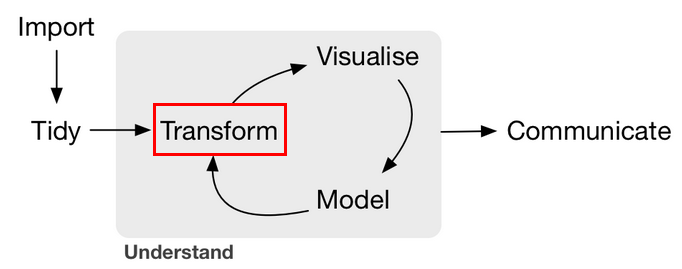
\includegraphics[width=0.75\textwidth]{../img/02_ciclo_3.png}
    \caption{Transformación de datos \textcite[Introducción]{grolemund2016r}.}
    \label{fig:ciclo3}
\end{figure}

Existen muchas maneras de transformar los datos y una gran cantidad de
paquetes que implementan distintas funciones útiles para realizar esta
tarea. En particular, resaltamos \texttt{dplyr} y \texttt{data.table}.
En esta sección se ejemplifican todas las funciones que permiten hacer
trabajo con datos que están implementadas en
\texttt{dplyr}\footnote{Para iniciar en \texttt{data.table} se recomienda ver \textcite{datatabletutorial} así como las viñetas del paquete \textcite{datatable}.}
y en \texttt{tidyr} \parencite{tidyr}.

\subsection{Tareas comunes en la manipulación de
datos}\label{tareas-comunes-en-la-manipulacion-de-datos}

Las funciones implementadas en este paquete están diseñadas para
facilitar la transformación de datos. En general, la transformación de
datos implica definir qué se hará con ellos, escribir un programa que
realice esa tarea y ejecutarlo
\parencite[][viñeta de introducción]{dplyr}.

\texttt{dplyr} y \texttt{tidyr} simplifican estos pasos al proveer de
opciones limitadas consideradas como las tareas más comunes en la
transformación de datos. Además, proveen de verbos simples que
corresponden a funciones en \texttt{R} y que mapean directamente a estas
\emph{tareas más comunes} (ver Tabla \ref{tab:accionescomunes}).

\begin{table}[H]
\centering
\scriptsize{
\begin{tabular}{p{4cm}p{10cm}}
  \hline
Acción & Verbos \\ 
\hline
Extracción de \textbf{subconjuntos de observaciones}. & 
  \parbox[t]{10cm}{
    \begin{itemize} 
      \item{\texttt{filter}: seleccionamos filas de acuerdo a los valores de las variables} 
      \item{\texttt{distinct}: elimina renglones duplicados}
      \item{\texttt{sample\_frac}: selecciona aleatoriamente una fracción de filas}
      \item{\texttt{sample\_n}: selecciona aleatoriamente $n$ filas}
      \item{\texttt{slice}: selecciona filas por posición}
      \item{\texttt{top\_n}: selecciona y ordena según una variable $n$ entradas\\}
    \end{itemize} 
  } \\
\hline
Extracción de \textbf{subconjuntos de variables}. &  
  \parbox[t]{10cm}{
    \begin{itemize} 
      \item{\texttt{select}: seleccionamos un subconjunto de las columnas utilizando los nombres de las variables\\}
    \end{itemize} 
  } \\
\hline
Creación de \textbf{resumenes de datos}. & 
  \parbox[t]{10cm}{
    \begin{itemize} 
      \item{\texttt{summarise}: resume los datos en un valor único}
      \item{\texttt{summarise\_each}: aplica una función de resumen a cada columna}
      \item{\texttt{count}: cuenta el número de filas con cada valor única de una variable\\}
    \end{itemize} 
  } \\
\hline
Creación de \textbf{nuevas variables}. &
  \parbox[t]{10cm}{
    \begin{itemize} 
      \item{\texttt{mutate}: genera nuevas variables a partir de las variables originales}
      \item{\texttt{mutate\_each}: aplica una función ventana a cada columna}
      \item{\texttt{transmute}: genera una o más nuevas columnas eliminando las columnas originales\\}
    \end{itemize} 
  } \\
\hline
\textbf{Combinación} de conjuntos de datos. & 
  \parbox[t]{10cm}{
    \begin{itemize} 
      \item{\texttt{left\_join}: realiza un join conservando todas las observaciones de la primera tabla especificada}
      \item{\texttt{right\_join}: realiza un join conservando todas las observaciones de la segunda tabla especificada}
      \item{\texttt{inner\_join}: realiza un join conservando todas las observaciones que están en ambas tablas}
      \item{\texttt{full\_join}: realiza un join conservando todas las observaciones y valores de ambas tablas}
      \item{\texttt{semi\_join}: conserva todas las observaciones de la primera tabla que están en la segunda tabla}
      \item{\texttt{anti\_join}: conserva todas las observaciones de la primera tabla que no están en la segunda tabla}
      \item{\texttt{intersect}: conserva observaciones que están tanto en la primera tabla como en la segunda}
      \item{\texttt{union}: conserva observaciones que están en cualesquier tabla}
      \item{\texttt{setdiff}: conserva observaciones de la primera tabla que no están en la segunda}
      \item{\texttt{bind\_rows}: une las filas de la segunda tabla a las de la primera}
      \item{\texttt{bind\_cols}: une las columnas de la segunda tabla a las de la primera\\}
    \end{itemize} 
  } \\
\hline
\textbf{Agrupar} datos. & 
  \parbox[t]{10cm}{
    \begin{itemize} 
      \item{\texttt{group\_by}: agrupa los datos según una o más variables}
      \item{\texttt{ungroup}: elimina los grupos en un data frame\\}
    \end{itemize} 
  } \\
\hline
\textbf{Reorganizar} datos (\textit{reshape data}). & 
  \parbox[t]{10cm}{
    \begin{itemize} 
      \item{\texttt{data\_frame}: combina vectores en un dataframe}
      \item{\texttt{arrange}: Ordena las filas según una o más variables}
      \item{\texttt{rename}: renombra columnas de un dataframe\\}
    \end{itemize} 
  } \\
\hline
\end{tabular}
}
\caption{Acciones y verbos comunes en la manipulación de datos \parencite{datawrangling}.} 
\label{tab:accionescomunes}
\end{table}

Dentro de \texttt{tidyr} hay más verbos útiles para reorganizar datos
que se verán en la sección \ref{datos-limpios} junto con los
\emph{criterios de datos limpios} que proporcionan un sustento para la
conceptualización de la manipulación de datos eficiente en \texttt{R}.

Todos estos verbos funcionan de la misma manera (tienen la misma
estructura):

\begin{itemize}
\tightlist
\item
  El primer argumento de la función es un \emph{data.frame}
\item
  Los argumentos subsecuentes indican qué es lo que se debe hacer a ese
  \emph{data.frame}
\item
  Siempre regresa un \emph{data.frame}
\end{itemize}

A continuación, se ejemplifica el uso de los distintos verbos de la
tabla \ref{tab:accionescomunes}. Para esto, utilizaremos los siguientes
conjuntos de datos de muestra, todos disponibles en el paquete
\texttt{nycflights13} \parencite{flights}. Se leerán desde archivo de
texto plano para ejemplificar algunos elementos de la limpieza.

Nota como utilizamos la función del paquete \texttt{readr}
\texttt{read\_csv}. Esta es una nueva implementación de
\texttt{read.csv} pero mucho mas rápida.

\begin{Shaded}
\begin{Highlighting}[]
\NormalTok{flights <-}\StringTok{ }\KeywordTok{read_csv}\NormalTok{(}\StringTok{"data/flights.csv"}\NormalTok{)}
\NormalTok{flights}
\end{Highlighting}
\end{Shaded}

\begin{verbatim}
## # A tibble: 227,496 x 14
##                   date  hour minute   dep   arr dep_delay arr_delay
##                 <dttm> <int>  <int> <int> <int>     <int>     <int>
##  1 2011-01-01 12:00:00    14      0  1400  1500         0       -10
##  2 2011-01-02 12:00:00    14      1  1401  1501         1        -9
##  3 2011-01-03 12:00:00    13     52  1352  1502        -8        -8
##  4 2011-01-04 12:00:00    14      3  1403  1513         3         3
##  5 2011-01-05 12:00:00    14      5  1405  1507         5        -3
##  6 2011-01-06 12:00:00    13     59  1359  1503        -1        -7
##  7 2011-01-07 12:00:00    13     59  1359  1509        -1        -1
##  8 2011-01-08 12:00:00    13     55  1355  1454        -5       -16
##  9 2011-01-09 12:00:00    14     43  1443  1554        43        44
## 10 2011-01-10 12:00:00    14     43  1443  1553        43        43
## # ... with 227,486 more rows, and 7 more variables: carrier <chr>,
## #   flight <int>, dest <chr>, plane <chr>, cancelled <int>, time <int>,
## #   dist <int>
\end{verbatim}

\begin{Shaded}
\begin{Highlighting}[]
\NormalTok{planes <-}\StringTok{ }\KeywordTok{read_csv}\NormalTok{(}\StringTok{"data/planes.csv"}\NormalTok{)}
\NormalTok{planes}
\end{Highlighting}
\end{Shaded}

\begin{verbatim}
## # A tibble: 2,853 x 9
##     plane  year               mfr          model no.eng no.seats speed
##     <chr> <int>             <chr>          <chr>  <int>    <int> <int>
##  1 N576AA  1991 MCDONNELL DOUGLAS DC-9-82(MD-82)      2      172    NA
##  2 N557AA  1993        MARZ BARRY      KITFOX IV      1        2    NA
##  3 N403AA  1974             RAVEN           S55A     NA        1    60
##  4 N492AA  1989 MCDONNELL DOUGLAS DC-9-82(MD-82)      2      172    NA
##  5 N262AA  1985 MCDONNELL DOUGLAS DC-9-82(MD-82)      2      172    NA
##  6 N493AA  1989 MCDONNELL DOUGLAS DC-9-82(MD-82)      2      172    NA
##  7 N477AA  1988 MCDONNELL DOUGLAS DC-9-82(MD-82)      2      172    NA
##  8 N476AA  1988 MCDONNELL DOUGLAS DC-9-82(MD-82)      2      172    NA
##  9 N504AA    NA AUTHIER ANTHONY P      TIERRA II      1        2    NA
## 10 N565AA  1987 MCDONNELL DOUGLAS DC-9-83(MD-83)      2      172    NA
## # ... with 2,843 more rows, and 2 more variables: engine <chr>, type <chr>
\end{verbatim}

\begin{Shaded}
\begin{Highlighting}[]
\NormalTok{airports <-}\StringTok{ }\KeywordTok{read_csv}\NormalTok{(}\StringTok{"data/airports.csv"}\NormalTok{)}
\NormalTok{airports}
\end{Highlighting}
\end{Shaded}

\begin{verbatim}
## # A tibble: 3,376 x 7
##     iata              airport             city state country      lat
##    <chr>                <chr>            <chr> <chr>   <chr>    <dbl>
##  1   00M              Thigpen      Bay Springs    MS     USA 31.95376
##  2   00R Livingston Municipal       Livingston    TX     USA 30.68586
##  3   00V          Meadow Lake Colorado Springs    CO     USA 38.94575
##  4   01G         Perry-Warsaw            Perry    NY     USA 42.74135
##  5   01J     Hilliard Airpark         Hilliard    FL     USA 30.68801
##  6   01M    Tishomingo County          Belmont    MS     USA 34.49167
##  7   02A           Gragg-Wade          Clanton    AL     USA 32.85049
##  8   02C              Capitol       Brookfield    WI     USA 43.08751
##  9   02G    Columbiana County   East Liverpool    OH     USA 40.67331
## 10   03D     Memphis Memorial          Memphis    MO     USA 40.44726
## # ... with 3,366 more rows, and 1 more variables: long <dbl>
\end{verbatim}

\subsection{Extracción de subconjuntos de
observaciones}\label{extraccion-de-subconjuntos-de-observaciones}

\subsubsection{filter}\label{filter}

Ya habíamos visto muchas maneras de extraer datos específicos de una
base de datos de acuerdo a condiciones lógicas impuestas en los valores
de las filas de columnas especificas. \texttt{filter} nos permite poner
tantas condiciones como queramos de manera muy fácil y entendible por
cualquiera que lea nuestro código.

Busquemos, por ejemplo, todos los vuelos hacia SFO u OAK

\begin{Shaded}
\begin{Highlighting}[]
\KeywordTok{filter}\NormalTok{(flights, dest }\OperatorTok{==}\StringTok{ "SFO"} \OperatorTok{|}\StringTok{ }\NormalTok{dest }\OperatorTok{==}\StringTok{ "OAK"}\NormalTok{)}
\end{Highlighting}
\end{Shaded}

\begin{verbatim}
## # A tibble: 3,508 x 14
##                   date  hour minute   dep   arr dep_delay arr_delay
##                 <dttm> <int>  <int> <int> <int>     <int>     <int>
##  1 2011-01-31 12:00:00     8     51   851  1052         1       -27
##  2 2011-01-31 12:00:00    11     29  1129  1351         4         1
##  3 2011-01-31 12:00:00    14     32  1432  1656         7         5
##  4 2011-01-31 12:00:00    17     48  1748  2001         3        -4
##  5 2011-01-31 12:00:00    21     43  2143  2338        50        24
##  6 2011-01-31 12:00:00     7     29   729  1002        -1         2
##  7 2011-01-31 12:00:00    15     58  1558  1812        -2        -8
##  8 2011-01-30 12:00:00     9     35   935  1203        45        49
##  9 2011-01-30 12:00:00    11     43  1143  1359        18        14
## 10 2011-01-30 12:00:00    14     59  1459  1715        34        24
## # ... with 3,498 more rows, and 7 more variables: carrier <chr>,
## #   flight <int>, dest <chr>, plane <chr>, cancelled <int>, time <int>,
## #   dist <int>
\end{verbatim}

Los vuelos con retraso mayor a 5 horas

\begin{Shaded}
\begin{Highlighting}[]
\KeywordTok{filter}\NormalTok{(flights, arr_delay }\OperatorTok{>}\StringTok{ }\DecValTok{5}\NormalTok{)}
\end{Highlighting}
\end{Shaded}

\begin{verbatim}
## # A tibble: 77,848 x 14
##                   date  hour minute   dep   arr dep_delay arr_delay
##                 <dttm> <int>  <int> <int> <int>     <int>     <int>
##  1 2011-01-09 12:00:00    14     43  1443  1554        43        44
##  2 2011-01-10 12:00:00    14     43  1443  1553        43        43
##  3 2011-01-11 12:00:00    14     29  1429  1539        29        29
##  4 2011-01-17 12:00:00    15     30  1530  1634        90        84
##  5 2011-01-20 12:00:00    15      7  1507  1622        67        72
##  6 2011-01-31 12:00:00    14     41  1441  1553        41        43
##  7 2011-01-13 12:00:00     7     22   722   841         2         6
##  8 2011-01-16 12:00:00     7     43   743   843        23         8
##  9 2011-01-17 12:00:00     7     24   724   842         4         7
## 10 2011-01-24 12:00:00     7     31   731   904        11        29
## # ... with 77,838 more rows, and 7 more variables: carrier <chr>,
## #   flight <int>, dest <chr>, plane <chr>, cancelled <int>, time <int>,
## #   dist <int>
\end{verbatim}

Podemos juntar las preguntas: vuelos con retraso mayor a 5 horas con
destino a SFO o OAK

\begin{Shaded}
\begin{Highlighting}[]
\KeywordTok{filter}\NormalTok{(flights, dest }\OperatorTok{==}\StringTok{ "SFO"} \OperatorTok{|}\StringTok{ }\NormalTok{dest }\OperatorTok{==}\StringTok{ "OAK"}\NormalTok{, arr_delay }\OperatorTok{>}\StringTok{ }\DecValTok{5}\NormalTok{)}
\end{Highlighting}
\end{Shaded}

\begin{verbatim}
## # A tibble: 1,581 x 14
##                   date  hour minute   dep   arr dep_delay arr_delay
##                 <dttm> <int>  <int> <int> <int>     <int>     <int>
##  1 2011-01-31 12:00:00    21     43  2143  2338        50        24
##  2 2011-01-30 12:00:00     9     35   935  1203        45        49
##  3 2011-01-30 12:00:00    11     43  1143  1359        18        14
##  4 2011-01-30 12:00:00    14     59  1459  1715        34        24
##  5 2011-01-30 12:00:00    17     49  1749  2011         4         6
##  6 2011-01-30 12:00:00    19     31  1931  2159        41        41
##  7 2011-01-30 12:00:00    21      0  2100  2320        10         9
##  8 2011-01-29 12:00:00     8     52   852  1126         2        12
##  9 2011-01-29 12:00:00    14     42  1442  1655        17         9
## 10 2011-01-29 12:00:00    18      9  1809  2021        14        11
## # ... with 1,571 more rows, and 7 more variables: carrier <chr>,
## #   flight <int>, dest <chr>, plane <chr>, cancelled <int>, time <int>,
## #   dist <int>
\end{verbatim}

\subsubsection{distinct}\label{distinct}

Para eliminar duplicados, usamos la función \texttt{distinct}

\begin{Shaded}
\begin{Highlighting}[]
\NormalTok{flights.dup <-}\StringTok{ }\KeywordTok{bind_rows}\NormalTok{(flights, flights)}
\KeywordTok{dim}\NormalTok{(flights.dup)}
\end{Highlighting}
\end{Shaded}

\begin{verbatim}
## [1] 454992     14
\end{verbatim}

\begin{Shaded}
\begin{Highlighting}[]
\KeywordTok{dim}\NormalTok{(}\KeywordTok{distinct}\NormalTok{(flights.dup))}
\end{Highlighting}
\end{Shaded}

\begin{verbatim}
## [1] 227496     14
\end{verbatim}

\begin{Shaded}
\begin{Highlighting}[]
\KeywordTok{rm}\NormalTok{(flights.dup)}
\end{Highlighting}
\end{Shaded}

\subsubsection{sample\_n, sample\_frac,
slice}\label{sample_n-sample_frac-slice}

En ocasiones necesitamos extraer subconjuntos aleatorios de los datos,
para ello podemos especificar el número de renglones que necesitamos
(usando \texttt{sample\_n}), el porcentaje de datos que deseamos (usando
\texttt{sample\_frac}) o las posiciones específicas de los datos que
queremos (usando \texttt{slice}).

\begin{Shaded}
\begin{Highlighting}[]
\KeywordTok{set.seed}\NormalTok{(}\DecValTok{1099}\NormalTok{) }
\CommentTok{# extraemos 10 datos en forma aleatoria}
\KeywordTok{sample_n}\NormalTok{(flights, }\DataTypeTok{size =} \DecValTok{10}\NormalTok{)}
\end{Highlighting}
\end{Shaded}

\begin{verbatim}
## # A tibble: 10 x 14
##                   date  hour minute   dep   arr dep_delay arr_delay
##                 <dttm> <int>  <int> <int> <int>     <int>     <int>
##  1 2011-05-29 12:00:00    12      3  1203  1304        -2       -16
##  2 2011-05-30 12:00:00    13     43  1343  1432        -2        -8
##  3 2011-07-20 12:00:00    18     21  1821  1956        10        20
##  4 2011-07-10 12:00:00    13      5  1305  1355         5         0
##  5 2011-06-17 12:00:00    11     30  1130  1228         5         3
##  6 2011-12-03 12:00:00     7     59   759   851        -1        -9
##  7 2011-06-12 12:00:00     9     19   919  1015         4         4
##  8 2011-09-24 12:00:00     7     55   755  1124        -5        -5
##  9 2011-04-19 12:00:00    17     48  1748     6        18        NA
## 10 2011-10-10 12:00:00    10     26  1026  1406         1        -1
## # ... with 7 more variables: carrier <chr>, flight <int>, dest <chr>,
## #   plane <chr>, cancelled <int>, time <int>, dist <int>
\end{verbatim}

\begin{Shaded}
\begin{Highlighting}[]
\CommentTok{# Extraemos el 1% de los datos de flights}
\KeywordTok{sample_frac}\NormalTok{(flights, }\DataTypeTok{size =} \FloatTok{0.01}\NormalTok{)}
\end{Highlighting}
\end{Shaded}

\begin{verbatim}
## # A tibble: 2,275 x 14
##                   date  hour minute   dep   arr dep_delay arr_delay
##                 <dttm> <int>  <int> <int> <int>     <int>     <int>
##  1 2011-03-21 12:00:00    13     21  1321  1635         6         0
##  2 2011-06-17 12:00:00    21      2  2102  2151         2        11
##  3 2011-07-12 12:00:00    10     17  1017  1448         2         1
##  4 2011-08-08 12:00:00    10     55  1055  1422         0        -3
##  5 2011-09-13 12:00:00    19      1  1901  2314        -4        -5
##  6 2011-03-06 12:00:00    18     32  1832  2044        -3       -11
##  7 2011-05-09 12:00:00     6     53   653   843        18       -15
##  8 2011-10-06 12:00:00    15     33  1533  1628         3        -7
##  9 2011-06-17 12:00:00    13     50  1350  1545         0         2
## 10 2011-11-01 12:00:00    14     30  1430  1601         5         1
## # ... with 2,265 more rows, and 7 more variables: carrier <chr>,
## #   flight <int>, dest <chr>, plane <chr>, cancelled <int>, time <int>,
## #   dist <int>
\end{verbatim}

\begin{Shaded}
\begin{Highlighting}[]
\CommentTok{# extraemos las posiciones 100 a 110}
\KeywordTok{slice}\NormalTok{(flights, }\DecValTok{100}\OperatorTok{:}\DecValTok{110}\NormalTok{)}
\end{Highlighting}
\end{Shaded}

\begin{verbatim}
## # A tibble: 11 x 14
##                   date  hour minute   dep   arr dep_delay arr_delay
##                 <dttm> <int>  <int> <int> <int>     <int>     <int>
##  1 2011-01-12 12:00:00    16     31  1631  1739         1        -6
##  2 2011-01-13 12:00:00    16     30  1630  1733         0       -12
##  3 2011-01-14 12:00:00    16     29  1629  1734        -1       -11
##  4 2011-01-15 12:00:00    16     32  1632  1736         2        -9
##  5 2011-01-16 12:00:00    17      8  1708  1819        38        34
##  6 2011-01-17 12:00:00    16     32  1632  1744         2        -1
##  7 2011-01-18 12:00:00    16     25  1625  1740        -5        -5
##  8 2011-01-19 12:00:00    16     29  1629  1731        -1       -14
##  9 2011-01-20 12:00:00    16     41  1641  1752        11         7
## 10 2011-01-21 12:00:00    16     38  1638  1746         8         1
## 11 2011-01-22 12:00:00    16     23  1623  1742        -7        -3
## # ... with 7 more variables: carrier <chr>, flight <int>, dest <chr>,
## #   plane <chr>, cancelled <int>, time <int>, dist <int>
\end{verbatim}

\subsubsection{top\_n}\label{top_n}

Podemos obtener los 5 vuelos con mayor retraso de salida:

\begin{Shaded}
\begin{Highlighting}[]
\KeywordTok{top_n}\NormalTok{(flights, }\DecValTok{5}\NormalTok{, dep_delay)}
\end{Highlighting}
\end{Shaded}

\begin{verbatim}
## # A tibble: 5 x 14
##                  date  hour minute   dep   arr dep_delay arr_delay carrier
##                <dttm> <int>  <int> <int> <int>     <int>     <int>   <chr>
## 1 2011-06-21 12:00:00    23     34  2334   124       869       861      UA
## 2 2011-06-09 12:00:00    20     29  2029  2243       814       793      MQ
## 3 2011-08-01 12:00:00     1     56   156   452       981       957      CO
## 4 2011-11-08 12:00:00     7     21   721   948       931       918      MQ
## 5 2011-12-12 12:00:00     6     50   650   808       970       978      AA
## # ... with 6 more variables: flight <int>, dest <chr>, plane <chr>,
## #   cancelled <int>, time <int>, dist <int>
\end{verbatim}

O con el menor retraso de salida:

\begin{Shaded}
\begin{Highlighting}[]
\KeywordTok{top_n}\NormalTok{(flights, }\DecValTok{5}\NormalTok{, }\KeywordTok{desc}\NormalTok{(dep_delay))}
\end{Highlighting}
\end{Shaded}

\begin{verbatim}
## # A tibble: 6 x 14
##                  date  hour minute   dep   arr dep_delay arr_delay carrier
##                <dttm> <int>  <int> <int> <int>     <int>     <int>   <chr>
## 1 2011-01-18 12:00:00    15     42  1542  1936       -18       -17      CO
## 2 2011-02-14 12:00:00    19     17  1917  2027       -23       -23      MQ
## 3 2011-04-10 12:00:00    21      1  2101  2206       -19       -12      XE
## 4 2011-08-03 12:00:00    17     41  1741  1810       -19       -40      XE
## 5 2011-10-04 12:00:00    14     38  1438  1813       -18       -31      EV
## 6 2011-12-24 12:00:00    11     12  1112  1314       -33       -25      OO
## # ... with 6 more variables: flight <int>, dest <chr>, plane <chr>,
## #   cancelled <int>, time <int>, dist <int>
\end{verbatim}

\subsection{\texorpdfstring{Extracción de subconjuntos de variables
(\emph{select})}{Extracción de subconjuntos de variables (select)}}\label{extraccion-de-subconjuntos-de-variables-select}

Podemos ahora, mas fácilmente, quedarnos con únicamente ciertas
variables. \texttt{select} esta implementado de tal manera que funciona
\emph{nombrando} las variables que se quieren utilizar.

\begin{Shaded}
\begin{Highlighting}[]
\KeywordTok{select}\NormalTok{(flights, flight, dest)}
\end{Highlighting}
\end{Shaded}

\begin{verbatim}
## # A tibble: 227,496 x 2
##    flight  dest
##     <int> <chr>
##  1    428   DFW
##  2    428   DFW
##  3    428   DFW
##  4    428   DFW
##  5    428   DFW
##  6    428   DFW
##  7    428   DFW
##  8    428   DFW
##  9    428   DFW
## 10    428   DFW
## # ... with 227,486 more rows
\end{verbatim}

También podemos especificar que queremos todas las variables
\emph{menos} algunas.

\begin{Shaded}
\begin{Highlighting}[]
\KeywordTok{select}\NormalTok{(flights, }\OperatorTok{-}\NormalTok{date, }\OperatorTok{-}\NormalTok{hour, }\OperatorTok{-}\NormalTok{minute, }\OperatorTok{-}\NormalTok{dep, }\OperatorTok{-}\NormalTok{arr, }\OperatorTok{-}\NormalTok{carrier, }\OperatorTok{-}\NormalTok{flight)}
\end{Highlighting}
\end{Shaded}

\begin{verbatim}
## # A tibble: 227,496 x 7
##    dep_delay arr_delay  dest  plane cancelled  time  dist
##        <int>     <int> <chr>  <chr>     <int> <int> <int>
##  1         0       -10   DFW N576AA         0    40   224
##  2         1        -9   DFW N557AA         0    45   224
##  3        -8        -8   DFW N541AA         0    48   224
##  4         3         3   DFW N403AA         0    39   224
##  5         5        -3   DFW N492AA         0    44   224
##  6        -1        -7   DFW N262AA         0    45   224
##  7        -1        -1   DFW N493AA         0    43   224
##  8        -5       -16   DFW N477AA         0    40   224
##  9        43        44   DFW N476AA         0    41   224
## 10        43        43   DFW N504AA         0    45   224
## # ... with 227,486 more rows
\end{verbatim}

Podemos pedir las variables que empiezan con algún caracter.

\begin{Shaded}
\begin{Highlighting}[]
\KeywordTok{select}\NormalTok{(flights, }\KeywordTok{starts_with}\NormalTok{(}\StringTok{"d"}\NormalTok{))}
\end{Highlighting}
\end{Shaded}

\begin{verbatim}
## # A tibble: 227,496 x 5
##                   date   dep dep_delay  dest  dist
##                 <dttm> <int>     <int> <chr> <int>
##  1 2011-01-01 12:00:00  1400         0   DFW   224
##  2 2011-01-02 12:00:00  1401         1   DFW   224
##  3 2011-01-03 12:00:00  1352        -8   DFW   224
##  4 2011-01-04 12:00:00  1403         3   DFW   224
##  5 2011-01-05 12:00:00  1405         5   DFW   224
##  6 2011-01-06 12:00:00  1359        -1   DFW   224
##  7 2011-01-07 12:00:00  1359        -1   DFW   224
##  8 2011-01-08 12:00:00  1355        -5   DFW   224
##  9 2011-01-09 12:00:00  1443        43   DFW   224
## 10 2011-01-10 12:00:00  1443        43   DFW   224
## # ... with 227,486 more rows
\end{verbatim}

O las que contienen algún patrón

\begin{Shaded}
\begin{Highlighting}[]
\KeywordTok{select}\NormalTok{(flights, }\KeywordTok{contains}\NormalTok{(}\StringTok{"dep"}\NormalTok{))}
\end{Highlighting}
\end{Shaded}

\begin{verbatim}
## # A tibble: 227,496 x 2
##      dep dep_delay
##    <int>     <int>
##  1  1400         0
##  2  1401         1
##  3  1352        -8
##  4  1403         3
##  5  1405         5
##  6  1359        -1
##  7  1359        -1
##  8  1355        -5
##  9  1443        43
## 10  1443        43
## # ... with 227,486 more rows
\end{verbatim}

\renewcommand\bcStyleTitre[1]{\large\textcolor{bbblack}{#1}}

\begin{bclogo}[
  couleur=llred,
  arrondi=0,
  logo=\bcstop,
  barre=none,
  noborder=true]{Ejercicios}
\begin{enumerate}
\item{Revisa la ayuda de select con \texttt{?select}.}
\item Juega con la función \texttt{starts\_with()}. ¿Qué variables empiezan con ``de''?
\item Juega con la función \texttt{ends\_with()}. ¿Qué variables terminan con ``delay''?
\item Utiliza la base de datos \texttt{iris} como en el ejemplo de la ayuda.
\item ¿Qué hace la función \texttt{contains()}?
\item ¿Cómo es diferente de \texttt{matches()}?
\item ¿Cómo obtienes todas las variables \textit{menos} Petal.Width?
\end{enumerate}
\end{bclogo}

\subsection{Creación de resumenes de
datos}\label{creacion-de-resumenes-de-datos}

Las funciones \texttt{summarise}, \texttt{summarise\_each} y
\texttt{count} permiten realizar resumenes para ciertas variables
existentes o nuevas en los datos.

\subsubsection{summarise}\label{summarise}

Ahora, si queremos saber el promedio de velocidad de los vuelos podemos
calcularlo fácilmente con \texttt{summarise}.

\begin{Shaded}
\begin{Highlighting}[]
\NormalTok{flights}\OperatorTok{$}\NormalTok{velocidad <-}\StringTok{ }\NormalTok{flights}\OperatorTok{$}\NormalTok{dist}\OperatorTok{/}\NormalTok{flights}\OperatorTok{$}\NormalTok{time}

\KeywordTok{summarise}\NormalTok{(flights, }\DataTypeTok{vel_prom =} \KeywordTok{mean}\NormalTok{(velocidad, }\DataTypeTok{na.rm =}\NormalTok{ T))}
\end{Highlighting}
\end{Shaded}

\begin{verbatim}
## # A tibble: 1 x 1
##   vel_prom
##      <dbl>
## 1 7.017055
\end{verbatim}

\begin{curiosidad}[Funciones resumen]
Pueden utilizarse junto con summarise cualesquiera función en \texttt{R} 
(por ejemplo: min, max, mean, median, var, sd) que
realice agregaciones de vectores. Sin embargo, el paquete \texttt{dplyr} implementa
varias funciones útiles adicionales como \parencite{datawrangling}: \\

\begin{itemize}
\item \texttt{first}: extrae el primer valor de un vector
\item \texttt{last}: extrae el último valor de un vector
\item \texttt{n}: cuenta el número de valores en un vector
\item \texttt{n\_distinct} cuenta el número de valores único en un vector
\end{itemize}
\end{curiosidad}

\subsubsection{summarise\_each}\label{summarise_each}

Podemos especificar una función a aplicar a variables específicas en un
dataframe. Por ejemplo, extraer la media para las variables: date,
dep\_delay, arr\_delay, time y dist.

\begin{Shaded}
\begin{Highlighting}[]
\KeywordTok{summarise_each}\NormalTok{(flights, }\KeywordTok{funs}\NormalTok{(mean), date, dep_delay, arr_delay, time, dist)}
\end{Highlighting}
\end{Shaded}

\begin{verbatim}
## # A tibble: 1 x 5
##                  date dep_delay arr_delay  time     dist
##                <dttm>     <dbl>     <dbl> <dbl>    <dbl>
## 1 2011-07-02 03:05:12        NA        NA    NA 787.7832
\end{verbatim}

Debido a que existen valores perdidos en variables como retraso de
salida (\emph{dep\_delay}) y retrasos de llegada (\emph{arr\_delay}),
debemos especificar la opción para no utilizar los NAs en la función.

\begin{Shaded}
\begin{Highlighting}[]
\KeywordTok{summarise_each}\NormalTok{(flights, }\KeywordTok{funs}\NormalTok{(}\KeywordTok{mean}\NormalTok{(., }\DataTypeTok{na.rm =}\NormalTok{ T)), date, dep_delay}
\NormalTok{               , arr_delay, time, dist)}
\end{Highlighting}
\end{Shaded}

\begin{verbatim}
## # A tibble: 1 x 5
##                  date dep_delay arr_delay     time     dist
##                <dttm>     <dbl>     <dbl>    <dbl>    <dbl>
## 1 2011-07-02 03:05:12  9.444951  7.094334 108.1423 787.7832
\end{verbatim}

\begin{Shaded}
\begin{Highlighting}[]
\CommentTok{# opcion 2}
\NormalTok{mean_na <-}\StringTok{ }\ControlFlowTok{function}\NormalTok{(x)\{}
  \KeywordTok{mean}\NormalTok{(x, }\DataTypeTok{na.rm =}\NormalTok{ T)}
\NormalTok{\}}
\KeywordTok{summarise_each}\NormalTok{(flights, }\KeywordTok{funs}\NormalTok{(mean_na), date, dep_delay, arr_delay, time, dist)}
\end{Highlighting}
\end{Shaded}

\begin{verbatim}
## # A tibble: 1 x 5
##                  date dep_delay arr_delay     time     dist
##                <dttm>     <dbl>     <dbl>    <dbl>    <dbl>
## 1 2011-07-02 03:05:12  9.444951  7.094334 108.1423 787.7832
\end{verbatim}

\subsubsection{count}\label{count}

Podemos contar los valores únicos en variables categóricas, por ejemplo,
contar el número de vuelos por aerolínea:

\begin{Shaded}
\begin{Highlighting}[]
\KeywordTok{count}\NormalTok{(flights, carrier, }\DataTypeTok{sort =}\NormalTok{ T)}
\end{Highlighting}
\end{Shaded}

\begin{verbatim}
## # A tibble: 15 x 2
##    carrier     n
##      <chr> <int>
##  1      XE 73053
##  2      CO 70032
##  3      WN 45343
##  4      OO 16061
##  5      MQ  4648
##  6      US  4082
##  7      AA  3244
##  8      DL  2641
##  9      EV  2204
## 10      FL  2139
## 11      UA  2072
## 12      F9   838
## 13      B6   695
## 14      AS   365
## 15      YV    79
\end{verbatim}

\subsection{Creación de nuevas
variables}\label{creacion-de-nuevas-variables}

\subsubsection{mutate y transmute}\label{mutate-y-transmute}

Muchas veces lo que se desea es generar nuevas variables utilizando
funciones sobre las variables de la tabla.

Por ejemplo, queremos saber cual fue el vuelo mas rápido. Para esto
queremos calcular la velocidad promedio del vuelo.

\begin{Shaded}
\begin{Highlighting}[]
\KeywordTok{select}\NormalTok{(}\KeywordTok{arrange}\NormalTok{(}\KeywordTok{mutate}\NormalTok{(flights, }\DataTypeTok{velocidad =}\NormalTok{ dist}\OperatorTok{/}\NormalTok{time), }\KeywordTok{desc}\NormalTok{(velocidad)),}
\NormalTok{       flight, dest, velocidad)}
\end{Highlighting}
\end{Shaded}

\begin{verbatim}
## # A tibble: 227,496 x 3
##    flight  dest velocidad
##     <int> <chr>     <dbl>
##  1   1646   AUS  12.72727
##  2   5229   MEM  11.16667
##  3    944   CLT  10.74118
##  4   4634   HOB  10.65957
##  5    500   IND  10.30488
##  6    106   EWR  10.14493
##  7    644   CLE  10.10185
##  8   1074   CLE  10.10185
##  9   1054   EWR  10.07194
## 10   1424   DCA  10.06667
## # ... with 227,486 more rows
\end{verbatim}

Esta manera de transformar a los datos (utilizando varios de los verbos)
es confusa y difícil de leer. Es mas sencillo utilizar el operador
pipe\footnote{Para una explicación más detallada de la importancia de este operador en la simplificación de código, ver la nota del autor del paquete Stefan Milton en \textcite{simplermagrittr} y la viñeta \texttt{magrittr} dentro del paquete.}
de \texttt{R} implementado en el paquete \texttt{magrittr}, es decir,
\texttt{\%\textgreater{}\%} \parencite{magrittr}.

\begin{Shaded}
\begin{Highlighting}[]
\NormalTok{flights2 <-}\StringTok{ }\KeywordTok{mutate}\NormalTok{(flights, }\DataTypeTok{velocidad =}\NormalTok{ dist}\OperatorTok{/}\NormalTok{time) }\OperatorTok
\StringTok{              }\KeywordTok{arrange}\NormalTok{(., }\KeywordTok{desc}\NormalTok{(velocidad)) }\OperatorTok
\StringTok{              }\KeywordTok{select}\NormalTok{(., flight, dest, velocidad)}
\NormalTok{flights2}
\end{Highlighting}
\end{Shaded}

\begin{verbatim}
## # A tibble: 227,496 x 3
##    flight  dest velocidad
##     <int> <chr>     <dbl>
##  1   1646   AUS  12.72727
##  2   5229   MEM  11.16667
##  3    944   CLT  10.74118
##  4   4634   HOB  10.65957
##  5    500   IND  10.30488
##  6    106   EWR  10.14493
##  7    644   CLE  10.10185
##  8   1074   CLE  10.10185
##  9   1054   EWR  10.07194
## 10   1424   DCA  10.06667
## # ... with 227,486 more rows
\end{verbatim}

La lectura es mucho mas sencilla de esta forma pues se lee de manera
secuencial las transformaciones que se están realizando a los datos:

\begin{enumerate}
\def\labelenumi{\arabic{enumi}.}
\tightlist
\item
  Agrego la columna de velocidad a la base de datos de \texttt{flights},
  luego (operador pipe)
\item
  Ordeno los vuelos en forma descendiente según su velocidad, luego
\item
  Selecciono las variables de vuelo, destino y velocidad.
\end{enumerate}

Que el código sea entendible no es importante únicamente en el contexto
del trabajo colaborativo pues muchas veces los lectores de su código
serán ustedes en el futuro.

\texttt{transmute} es muy similar a \texttt{mutate} pero elimina las
variables que no fueron creadas por la función.

\begin{Shaded}
\begin{Highlighting}[]
\NormalTok{dplyr}\OperatorTok{::}\KeywordTok{transmute}\NormalTok{(flights, }\DataTypeTok{velocidad =}\NormalTok{ dist}\OperatorTok{/}\NormalTok{time) }\OperatorTok
\StringTok{              }\KeywordTok{arrange}\NormalTok{(., }\KeywordTok{desc}\NormalTok{(velocidad)) }
\end{Highlighting}
\end{Shaded}

\begin{verbatim}
## # A tibble: 227,496 x 1
##    velocidad
##        <dbl>
##  1  12.72727
##  2  11.16667
##  3  10.74118
##  4  10.65957
##  5  10.30488
##  6  10.14493
##  7  10.10185
##  8  10.10185
##  9  10.07194
## 10  10.06667
## # ... with 227,486 more rows
\end{verbatim}

\renewcommand\bcStyleTitre[1]{\large\textcolor{bbblack}{#1}}

\begin{bclogo}[
  couleur=llred,
  arrondi=0,
  logo=\bcstop,
  barre=none,
  noborder=true]{Ejercicios}
\begin{enumerate}
\item ¿Cuáles son los 10 aviones-aerolíneas mas lentos? Utiliza el operador pipe, 
mutate, arrange y head.
\item Utiliza la función \texttt{str\_sub} dentro de \texttt{stringr} para extraer únicamente el 
día del campo \texttt{date}.
3. Utiliza la función \texttt{ymd} del paquete \texttt{lubridate} para declarar date como una
fecha (¡otra clase!).
4. Utiliza las funciones \texttt{paste0} del \texttt{base} y \texttt{ymd\_hm} de \texttt{lubridate} para
declarar date como un \texttt{datetime}.
\end{enumerate}
\end{bclogo}

\begin{Shaded}
\begin{Highlighting}[]
\CommentTok{# Respuestas}

\CommentTok{#1}
\KeywordTok{mutate}\NormalTok{(flights, }\DataTypeTok{velocidad =}\NormalTok{ dist}\OperatorTok{/}\NormalTok{time) }\OperatorTok
\StringTok{    }\KeywordTok{arrange}\NormalTok{(velocidad) }\OperatorTok
\StringTok{    }\KeywordTok{head}\NormalTok{(}\DecValTok{10}\NormalTok{) }\OperatorTok
\StringTok{    }\KeywordTok{select}\NormalTok{(plane, carrier, velocidad)}

\CommentTok{# Más lindo, usando group_by y top_n: más específicamente el más }
\CommentTok{# lento por carrier}
\KeywordTok{mutate}\NormalTok{(flights, }\DataTypeTok{velocidad =}\NormalTok{ dist}\OperatorTok{/}\NormalTok{time) }\OperatorTok
\StringTok{    }\KeywordTok{group_by}\NormalTok{(carrier) }\OperatorTok
\StringTok{    }\KeywordTok{arrange}\NormalTok{(velocidad) }\OperatorTok
\StringTok{    }\KeywordTok{top_n}\NormalTok{(}\DecValTok{1}\NormalTok{) }\OperatorTok
\StringTok{    }\KeywordTok{select}\NormalTok{(plane, carrier, velocidad)}

\CommentTok{#2}
\KeywordTok{mutate}\NormalTok{(flights, }\DataTypeTok{dia =}\NormalTok{ stringr}\OperatorTok{::}\KeywordTok{str_sub}\NormalTok{(date, }\DecValTok{9}\NormalTok{, }\DecValTok{10}\NormalTok{)) }\OperatorTok
\StringTok{    }\KeywordTok{select}\NormalTok{(date, dia)}
\KeywordTok{head}\NormalTok{(flights)}

\CommentTok{# 3}
\KeywordTok{mutate}\NormalTok{(flights,}
       \DataTypeTok{fecha =}\NormalTok{ stringr}\OperatorTok{::}\KeywordTok{str_sub}\NormalTok{(date, }\DecValTok{1}\NormalTok{, }\DecValTok{10}\NormalTok{)}
\NormalTok{       , }\DataTypeTok{fecha =}\NormalTok{ lubridate}\OperatorTok{::}\KeywordTok{ymd}\NormalTok{(fecha)) }\OperatorTok
\StringTok{    }\KeywordTok{select}\NormalTok{(date, fecha)}

\CommentTok{# 4}
\KeywordTok{mutate}\NormalTok{(flights,}
       \DataTypeTok{fecha =}\NormalTok{ lubridate}\OperatorTok{::}\KeywordTok{ymd_hms}\NormalTok{(date)) }\OperatorTok
\StringTok{    }\KeywordTok{select}\NormalTok{(date, fecha)}
\end{Highlighting}
\end{Shaded}

\begin{curiosidad}[Funciones ventana \textit{window functions}]
Dentro de mutate, se pueden utilizar otras funciones que realicen transformaciones
sobre vectores que regresen un vector del mismo tamaño, así como funciones
propias.\\

Ahora bien, \texttt{dplyr} implementa otras funciones ventana como \parencite{datawrangling}:\\

\begin{itemize}
\item \texttt{lead}: regresa todos los valores del vector movidos por una posición posterior
\item \texttt{lag}: regresa todos los valores del vector movidos por una posición anterior
\item \texttt{dense\_rank}: rango sin huecos
\item \texttt{min\_rank}: rango especificando el criterio de mínimo para empates
\item \texttt{percent\_rank}: rango reescalado para estar entre 0 y 1
\item \texttt{row\_number}: número de fila
\item \texttt{ntile}: creación de $n$ percentiles
\item \texttt{between}: verifica si el valor está entre dos valores
\item \texttt{cume\_dist}: distribución acumulada
\item \texttt{cumall}: para vectores lógicos, intersección de los valores al renglón i-ésimo
\item \texttt{cumany}: para vectores lógicos, unión de los valores al renglón i-ésimo
\item \texttt{cummean}: acumula la media \\
\end{itemize}

Para mayor detalle, puede revisarse la viñeta ``window-functions'' en el 
paquete dplyr \parencite{dplyr} con el comando \texttt{vignette("window-functions", package $=$ "dplyr")}
\end{curiosidad}

\subsubsection{mutate\_each}\label{mutate_each}

Igual que con \texttt{summarise\_each}, \texttt{mutate\_each} permite
especificar una transformación vía una función ventana para variables
específicas. Por ejemplo, extraemos los deciles correspondientes para
las variables tiempo (\emph{time}) y distancia (\emph{dist}).

\begin{Shaded}
\begin{Highlighting}[]
\NormalTok{flights.m <-}\StringTok{ }\KeywordTok{mutate_each}\NormalTok{(flights, }\KeywordTok{funs}\NormalTok{(}\KeywordTok{ntile}\NormalTok{(., }\DecValTok{10}\NormalTok{)), time, dist)}
\KeywordTok{table}\NormalTok{(flights.m}\OperatorTok{$}\NormalTok{time)}
\end{Highlighting}
\end{Shaded}

\begin{verbatim}
## 
##     1     2     3     4     5     6     7     8     9    10 
## 22388 22387 22388 22387 22387 22388 22387 22388 22387 22387
\end{verbatim}

\subsection{\texorpdfstring{Combinación de conjuntos de datos
(\emph{joins})}{Combinación de conjuntos de datos (joins)}}\label{combinacion-de-conjuntos-de-datos-joins}

Muchas veces la información se tiene repartida entre diferentes tablas
pero es necesario juntar las variables de las diferentes observaciones
en una sola tabla para modelarlas o describirlas. Es muy estándar, en el
lenguaje SQL, el tipo de joins que se pueden utilizar. La figura
\ref{fig:joins} muestra un resumen del tipo de joins que pueden
realizarse.

\begin{figure}[h]
    \centering
    \includegraphics[width=0.75\textwidth]{../img/02_joins.PNG}
    \caption{Joins en el lenguaje SQL \parencite{joins}.}
    \label{fig:joins}
\end{figure}

El paquete \texttt{dplyr} implementa estos joins de manera natural,
utilizando la lógica de SQL.

\begin{itemize}
\tightlist
\item
  \texttt{inner\_join}: regresa todas las filas de x en donde hay
  valores correspondientes para y, junto con todas las columnas.
\item
  \texttt{left\_join}: regresa todas las filas de x, rellenando con NA
  para valores que no encontró en y.
\item
  \texttt{right\_join}: regresa todas las filas de y, rellenando con NA
  para valores que no encontró en y.
\item
  \texttt{full\_join}: regresa todas las filas y todas las columnas para
  x y y. Donde no hay valores en alguno de los dos, rellena con NA.
\item
  \texttt{semi\_join}: regresa todas las filas de x para las que hay
  valores en y regresando únicamente las columnas de x.
\item
  \texttt{anti\_join}: regresa todas las filas de x donde no hay valores
  en y, manteniendo solo las columnas de x.
\end{itemize}

Ahora, supongamos que queremos saber la velocidad promedio de los
aviones que tenemos en nuestros datos para todos sus vuelos.

\begin{Shaded}
\begin{Highlighting}[]
\CommentTok{# base de aviones con velocidad}

\NormalTok{vel_aviones <-}\StringTok{ }\NormalTok{flights }\OperatorTok\StringTok{ }
\StringTok{  }\KeywordTok{group_by}\NormalTok{(plane) }\OperatorTok
\StringTok{  }\KeywordTok{summarise}\NormalTok{(}\DataTypeTok{vel_prom =} \KeywordTok{mean}\NormalTok{(dist}\OperatorTok{/}\NormalTok{time, }\DataTypeTok{na.rm =}\NormalTok{ T))}
  
\KeywordTok{inner_join}\NormalTok{(}
\NormalTok{  planes,}
\NormalTok{  vel_aviones}
\NormalTok{)  }\OperatorTok
\StringTok{  }\KeywordTok{select}\NormalTok{(plane, year, vel_prom) }\OperatorTok
\StringTok{  }\KeywordTok{arrange}\NormalTok{(}\KeywordTok{desc}\NormalTok{(vel_prom))}
\end{Highlighting}
\end{Shaded}

\begin{verbatim}
## # A tibble: 2,853 x 3
##     plane  year vel_prom
##     <chr> <int>    <dbl>
##  1 N653JB  2007 9.333333
##  2 N709UW  1999 9.316327
##  3 N3744F  2001 9.070175
##  4 N3769L  2002 9.065789
##  5 N623JB  2005 9.037975
##  6 N607JB  2005 8.936351
##  7 N580JB  2003 8.869907
##  8 N658JB  2007 8.869565
##  9 N589JB  2004 8.814815
## 10 N760JB  2008 8.788441
## # ... with 2,843 more rows
\end{verbatim}

Ahora, queremos saber los destinos con mayores retrasos.

\begin{Shaded}
\begin{Highlighting}[]
\NormalTok{destinos <-}\StringTok{ }\NormalTok{flights }\OperatorTok\StringTok{ }
\StringTok{  }\KeywordTok{group_by}\NormalTok{(dest) }\OperatorTok
\StringTok{  }\KeywordTok{summarise}\NormalTok{(}\DataTypeTok{retraso =} \KeywordTok{mean}\NormalTok{(arr_delay, }\DataTypeTok{na.rm =}\NormalTok{ T))}

\KeywordTok{inner_join}\NormalTok{(}
\NormalTok{  airports, }
\NormalTok{  destinos,}
  \DataTypeTok{by =} \KeywordTok{c}\NormalTok{(}\StringTok{"iata"}\NormalTok{ =}\StringTok{ "dest"}\NormalTok{)}
\NormalTok{) }\OperatorTok
\StringTok{  }\KeywordTok{arrange}\NormalTok{(}\KeywordTok{desc}\NormalTok{(retraso))}
\end{Highlighting}
\end{Shaded}

\begin{verbatim}
## # A tibble: 114 x 8
##     iata                             airport                 city state
##    <chr>                               <chr>                <chr> <chr>
##  1   ANC Ted Stevens Anchorage International            Anchorage    AK
##  2   CID                        Eastern Iowa         Cedar Rapids    IA
##  3   DSM            Des Moines International           Des Moines    IA
##  4   SFO         San Francisco International        San Francisco    CA
##  5   BPT            Southeast Texas Regional Beaumont/Port Arthur    TX
##  6   GRR           Kent County International         Grand Rapids    MI
##  7   DAY             James M Cox Dayton Intl               Dayton    OH
##  8   VPS                Eglin Air Force Base           Valparaiso    FL
##  9   SAV              Savannah International             Savannah    GA
## 10   RIC              Richmond International             Richmond    VA
## # ... with 104 more rows, and 4 more variables: country <chr>, lat <dbl>,
## #   long <dbl>, retraso <dbl>
\end{verbatim}

\subsection{Agrupar datos}\label{agrupar-datos}

\subsubsection{group\_by}\label{group_by}

Un verbo muy poderoso es el group\_by. Es por este tipo de verbos que
resultó necesario generar un objeto diferente al tradicional dataframe.
Básicamente, el tbl\_df es capaz de guardar agrupamientos específicos
sobre los cuáles puede hacer funciones ventana (\emph{window functions})
o resúmenes sobre los grupos que se definen.

\paragraph{Ejemplo}\label{ejemplo}

Los datos de vuelos se agrupan naturalmente sobre las aerolíneas.

\begin{Shaded}
\begin{Highlighting}[]
\NormalTok{flights.g <-}\StringTok{ }\NormalTok{flights }\OperatorTok\StringTok{ }\KeywordTok{group_by}\NormalTok{(., carrier)}
\NormalTok{flights.g}
\end{Highlighting}
\end{Shaded}

\begin{verbatim}
## Source: local data frame [227,496 x 15]
## Groups: carrier [15]
## 
## # A tibble: 227,496 x 15
##                   date  hour minute   dep   arr dep_delay arr_delay
##                 <dttm> <int>  <int> <int> <int>     <int>     <int>
##  1 2011-01-01 12:00:00    14      0  1400  1500         0       -10
##  2 2011-01-02 12:00:00    14      1  1401  1501         1        -9
##  3 2011-01-03 12:00:00    13     52  1352  1502        -8        -8
##  4 2011-01-04 12:00:00    14      3  1403  1513         3         3
##  5 2011-01-05 12:00:00    14      5  1405  1507         5        -3
##  6 2011-01-06 12:00:00    13     59  1359  1503        -1        -7
##  7 2011-01-07 12:00:00    13     59  1359  1509        -1        -1
##  8 2011-01-08 12:00:00    13     55  1355  1454        -5       -16
##  9 2011-01-09 12:00:00    14     43  1443  1554        43        44
## 10 2011-01-10 12:00:00    14     43  1443  1553        43        43
## # ... with 227,486 more rows, and 8 more variables: carrier <chr>,
## #   flight <int>, dest <chr>, plane <chr>, cancelled <int>, time <int>,
## #   dist <int>, velocidad <dbl>
\end{verbatim}

\renewcommand\bcStyleTitre[1]{\large\textcolor{bbblack}{#1}}

\begin{bclogo}[
  couleur=llred,
  arrondi=0,
  logo=\bcstop,
  barre=none,
  noborder=true]{Ejercicios}
\begin{enumerate}
\item Busca en la ayuda la función \texttt{top\_n}.
\item Utilízala, junto con \texttt{group\_by}, \texttt{arrange} y \texttt{summarise} para extraer los 10 
aviones por aerolínea con el menor promedio de velocidad.
\item ¿Cuáles son los aeropuertos con mayor promedio de retraso en la salida?
\item ¿Cuáles son los aeropuertos con mayor promedio de retraso en las llegadas?
\end{enumerate}

\end{bclogo}

\begin{Shaded}
\begin{Highlighting}[]
\CommentTok{# Respuestas}
\CommentTok{# 1}
\NormalTok{?top_n}
\CommentTok{# 2}
\NormalTok{flights }\OperatorTok
\StringTok{    }\KeywordTok{mutate}\NormalTok{(}\DataTypeTok{velocidad =}\NormalTok{ dist}\OperatorTok{/}\NormalTok{time) }\OperatorTok
\StringTok{    }\KeywordTok{group_by}\NormalTok{(plane, carrier) }\OperatorTok
\StringTok{    }\KeywordTok{summarise}\NormalTok{(}\DataTypeTok{vel_prom =} \KeywordTok{mean}\NormalTok{(velocidad, }\DataTypeTok{na.rm =}\NormalTok{ T)) }\OperatorTok
\StringTok{    }\KeywordTok{ungroup}\NormalTok{() }\OperatorTok
\StringTok{    }\KeywordTok{group_by}\NormalTok{(carrier) }\OperatorTok
\StringTok{    }\KeywordTok{arrange}\NormalTok{(vel_prom) }\OperatorTok
\StringTok{    }\KeywordTok{top_n}\NormalTok{(}\DecValTok{1}\NormalTok{) }

\CommentTok{# 3}
\NormalTok{flights }\OperatorTok
\StringTok{    }\KeywordTok{group_by}\NormalTok{(dest) }\OperatorTok
\StringTok{    }\KeywordTok{summarise}\NormalTok{(}\DataTypeTok{arr_delay =} \KeywordTok{mean}\NormalTok{(arr_delay, }\DataTypeTok{na.rm =}\NormalTok{ T)) }\OperatorTok
\StringTok{    }\KeywordTok{arrange}\NormalTok{(}\KeywordTok{desc}\NormalTok{(arr_delay)) }\OperatorTok
\StringTok{    }\KeywordTok{head}\NormalTok{(}\DecValTok{10}\NormalTok{)}
\end{Highlighting}
\end{Shaded}

\begin{curiosidad}[Afectación de otros verbos por \texttt{group\_by}]
El establecer grupos puede conjugarse con los demás verbos implementados en 
el paquete \texttt{dplyr} y los afecta de diferente manera \parencite[][viñeta de introducción]{dplyr}:\\

\begin{itemize}
\item \texttt{select} realiza la misma operación pero retiene siempre las variables de agrupación.
\item \texttt{arrange} realiza el arreglo según las variables especificadas pero ordena primero según los grupos.
\item \texttt{mutate} y \texttt{filter} realizan las operación dentro de los grupos definidos y son más útiles cuando se utilizan en conjunción a las funciones ventana.
\item \texttt{sample\_n} y \texttt{sample\_frac} extraen el número o fracción de observaciones según el número o fracción de filas en cada grupo.
\item \texttt{summarise} en conjunción con \texttt{group\_by} llevan acabo el paradigma split (por las variables definidas en el \texttt{group\_by}), apply (por las funciones especificadas en el \texttt{summarise}) y lo combinan en un dataframe.
\end{itemize}
\end{curiosidad}

\subsubsection{ungroup}\label{ungroup}

La función \texttt{group\_by} agrega la clase \texttt{grouped\_df}, así
como atributos al objeto.

\begin{Shaded}
\begin{Highlighting}[]
\NormalTok{g.df <-}\StringTok{ }\KeywordTok{group_by}\NormalTok{(flights, plane, carrier)}
\KeywordTok{class}\NormalTok{(g.df)}
\end{Highlighting}
\end{Shaded}

\begin{verbatim}
## [1] "grouped_df" "tbl_df"     "tbl"        "data.frame"
\end{verbatim}

\begin{Shaded}
\begin{Highlighting}[]
\KeywordTok{names}\NormalTok{(}\KeywordTok{attributes}\NormalTok{(g.df))}
\end{Highlighting}
\end{Shaded}

\begin{verbatim}
##  [1] "names"              "row.names"          "spec"              
##  [4] "class"              "vars"               "drop"              
##  [7] "indices"            "group_sizes"        "biggest_group_size"
## [10] "labels"
\end{verbatim}

\begin{Shaded}
\begin{Highlighting}[]
\KeywordTok{class}\NormalTok{(flights)}
\end{Highlighting}
\end{Shaded}

\begin{verbatim}
## [1] "tbl_df"     "tbl"        "data.frame"
\end{verbatim}

\begin{Shaded}
\begin{Highlighting}[]
\KeywordTok{names}\NormalTok{(}\KeywordTok{attributes}\NormalTok{(flights))}
\end{Highlighting}
\end{Shaded}

\begin{verbatim}
## [1] "names"     "row.names" "spec"      "class"
\end{verbatim}

La función \texttt{ungroup} los elimina:

\begin{Shaded}
\begin{Highlighting}[]
\KeywordTok{class}\NormalTok{(}\KeywordTok{ungroup}\NormalTok{(g.df))}
\end{Highlighting}
\end{Shaded}

\begin{verbatim}
## [1] "tbl_df"     "tbl"        "data.frame"
\end{verbatim}

\begin{Shaded}
\begin{Highlighting}[]
\KeywordTok{names}\NormalTok{(}\KeywordTok{attributes}\NormalTok{(}\KeywordTok{ungroup}\NormalTok{(g.df)))}
\end{Highlighting}
\end{Shaded}

\begin{verbatim}
## [1] "class"     "names"     "row.names" "spec"
\end{verbatim}

\renewcommand\bcStyleTitre[1]{\large\textcolor{bbblack}{#1}}

\begin{bclogo}[
  couleur=llred,
  arrondi=0,
  logo=\bcstop,
  barre=none,
  noborder=true]{Ejercicios}
\begin{enumerate}
\item ¿Cuáles son los aeropuertos que SI están en la base de destinos?
\item ¿Cuáles son los aeropuertos que NO están en la base de destinos?
\item Realiza un resumen de los vuelos por aeropuerto para varias variables con la función \texttt{summarise}.
\item Utiliza la función \texttt{inner\_join} para pegar la tablas de resumen creada en el paso anterior a la tabla \textit{airports}
\item Realiza un resumen de los vuelos por avión para varias variables con la función \texttt{summarise}.
\item Utiliza la función \texttt{left\_join} para pegar la tablas de resumen creada en el paso anterior a la tabla \textit{planes}
\item Extrae el porcentaje de vuelos cancelados por aerolínea cada año y el porcentaje de vuelos retrasados por aerolínea cada año.
\end{enumerate}

\end{bclogo}

\begin{Shaded}
\begin{Highlighting}[]
\CommentTok{# Respuestas}

\CommentTok{# 1}
\KeywordTok{semi_join}\NormalTok{(airports, flights, }\DataTypeTok{by =} \KeywordTok{c}\NormalTok{(}\StringTok{"iata"}\NormalTok{ =}\StringTok{ "dest"}\NormalTok{))}
\CommentTok{# 2}
\KeywordTok{anti_join}\NormalTok{(airports, flights, }\DataTypeTok{by =} \KeywordTok{c}\NormalTok{(}\StringTok{"iata"}\NormalTok{ =}\StringTok{ "dest"}\NormalTok{))}
\CommentTok{# 3}
\NormalTok{res.vuelos <-}\StringTok{ }\NormalTok{flights }\OperatorTok
\StringTok{  }\KeywordTok{group_by}\NormalTok{(dest) }\OperatorTok
\StringTok{  }\KeywordTok{summarise}\NormalTok{(}
    \DataTypeTok{flights =} \KeywordTok{n}\NormalTok{()}
\NormalTok{    , }\DataTypeTok{planes =} \KeywordTok{n_distinct}\NormalTok{(plane)}
\NormalTok{    , }\DataTypeTok{carriers =} \KeywordTok{n_distinct}\NormalTok{(carrier)}
\NormalTok{    , }\DataTypeTok{cancelled_flights =} \KeywordTok{sum}\NormalTok{(cancelled, }\DataTypeTok{na.rm =}\NormalTok{ T)}
\NormalTok{    , }\DataTypeTok{dep_delay_mean =} \KeywordTok{mean}\NormalTok{(dep_delay, }\DataTypeTok{na.rm =}\NormalTok{ T)}
\NormalTok{  )}
\CommentTok{# 4}
\NormalTok{airports_flights <-}\StringTok{ }\KeywordTok{inner_join}\NormalTok{(airports, res.vuelos}
\NormalTok{                               , }\DataTypeTok{by =} \KeywordTok{c}\NormalTok{(}\StringTok{"iata"}\NormalTok{ =}\StringTok{ "dest"}\NormalTok{))}
\CommentTok{# 5}
\NormalTok{res.aviones <-}\StringTok{ }\NormalTok{flights }\OperatorTok
\StringTok{  }\KeywordTok{group_by}\NormalTok{(plane) }\OperatorTok
\StringTok{  }\KeywordTok{summarise}\NormalTok{(}
    \DataTypeTok{flights =} \KeywordTok{n}\NormalTok{()}
\NormalTok{    , }\DataTypeTok{carriers =} \KeywordTok{n_distinct}\NormalTok{(carrier)}
\NormalTok{    , }\DataTypeTok{cancelled_flights =} \KeywordTok{sum}\NormalTok{(cancelled, }\DataTypeTok{na.rm =}\NormalTok{ T)}
\NormalTok{    , }\DataTypeTok{dep_delay_mean =} \KeywordTok{mean}\NormalTok{(dep_delay, }\DataTypeTok{na.rm =}\NormalTok{ T)}
\NormalTok{    , }\DataTypeTok{arr_delay_mean =} \KeywordTok{mean}\NormalTok{(arr_delay, }\DataTypeTok{na.rm =}\NormalTok{ T)}
\NormalTok{    , }\DataTypeTok{dist_mean =} \KeywordTok{mean}\NormalTok{(dist, }\DataTypeTok{na.rm =}\NormalTok{ T)}
\NormalTok{    , }\DataTypeTok{vel_mean =} \KeywordTok{mean}\NormalTok{(dist}\OperatorTok{/}\NormalTok{time, }\DataTypeTok{na.rm =}\NormalTok{ T)}
\NormalTok{  ) }
\CommentTok{# 6}
\NormalTok{planes_flights <-}\StringTok{ }\KeywordTok{left_join}\NormalTok{(planes, res.aviones)}
\CommentTok{# 7 }
\NormalTok{flights }\OperatorTok
\StringTok{  }\KeywordTok{mutate}\NormalTok{(}\DataTypeTok{anio =}\NormalTok{ lubridate}\OperatorTok{::}\KeywordTok{year}\NormalTok{(date)) }\OperatorTok
\StringTok{  }\KeywordTok{group_by}\NormalTok{(carrier, anio) }\OperatorTok
\StringTok{  }\KeywordTok{summarise}\NormalTok{(}
    \DataTypeTok{vuelos.anuales =} \KeywordTok{n}\NormalTok{()}
\NormalTok{    , }\DataTypeTok{cancelados =} \KeywordTok{sum}\NormalTok{(cancelled, }\DataTypeTok{na.rm =}\NormalTok{ T)}\OperatorTok{/}\NormalTok{vuelos.anuales }\OperatorTok{*}\StringTok{ }\DecValTok{100}
\NormalTok{    , }\DataTypeTok{retrasados =} \KeywordTok{sum}\NormalTok{(dep_delay }\OperatorTok{>}\StringTok{ }\DecValTok{0}\NormalTok{, }\DataTypeTok{na.rm =}\NormalTok{ T)}\OperatorTok{/}\NormalTok{vuelos.anuales }\OperatorTok{*}\StringTok{ }\DecValTok{100}
\NormalTok{  ) }\OperatorTok
\StringTok{  }\KeywordTok{ungroup}\NormalTok{()}
\end{Highlighting}
\end{Shaded}

\subsection{Reorganizar datos}\label{reorganizar-datos}

\subsubsection{data\_frame}\label{data_frame}

Al igual que la función \texttt{data.frame}, esta función permite
generar un data frame a partir de vectores:

\begin{Shaded}
\begin{Highlighting}[]
\NormalTok{df <-}\StringTok{ }\KeywordTok{data_frame}\NormalTok{(}
  \DataTypeTok{x =} \KeywordTok{rnorm}\NormalTok{(}\DecValTok{100}\NormalTok{)}
\NormalTok{  , }\DataTypeTok{y =} \KeywordTok{runif}\NormalTok{(}\DecValTok{100}\NormalTok{)}
\NormalTok{)}
\KeywordTok{class}\NormalTok{(df)}
\end{Highlighting}
\end{Shaded}

\begin{verbatim}
## [1] "tbl_df"     "tbl"        "data.frame"
\end{verbatim}

\begin{Shaded}
\begin{Highlighting}[]
\NormalTok{df <-}\StringTok{ }\KeywordTok{data.frame}\NormalTok{(}
  \DataTypeTok{x =} \KeywordTok{rnorm}\NormalTok{(}\DecValTok{100}\NormalTok{)}
\NormalTok{  , }\DataTypeTok{y =} \KeywordTok{runif}\NormalTok{(}\DecValTok{100}\NormalTok{)}
\NormalTok{)}
\KeywordTok{class}\NormalTok{(df)}
\end{Highlighting}
\end{Shaded}

\begin{verbatim}
## [1] "data.frame"
\end{verbatim}

La clase del objeto generado por la función \texttt{data\_frame} es un
\texttt{tibble} mientras que la función del base \texttt{data.frame} es
de clase \texttt{data.frame}.

\subsubsection{arrange}\label{arrange}

\texttt{order} habíamos visto que es la implementación del base para
ordenar vectores o en su defecto, dataframes de acuerdo a valores de
vectores en esta. Sin embargo, es engorrosa la manera de llamarlo.

Podemos arreglar los valores de las tablas, fácilmente con
\texttt{arrange}. Por ejemplo, podemos ver los 5 vuelos con mayor
retraso de llegada.

\begin{Shaded}
\begin{Highlighting}[]
\KeywordTok{head}\NormalTok{(}\KeywordTok{arrange}\NormalTok{(flights, }\KeywordTok{desc}\NormalTok{(arr_delay)), }\DataTypeTok{n=}\DecValTok{5}\NormalTok{)}
\end{Highlighting}
\end{Shaded}

\begin{verbatim}
## # A tibble: 5 x 15
##                  date  hour minute   dep   arr dep_delay arr_delay carrier
##                <dttm> <int>  <int> <int> <int>     <int>     <int>   <chr>
## 1 2011-12-12 12:00:00     6     50   650   808       970       978      AA
## 2 2011-08-01 12:00:00     1     56   156   452       981       957      CO
## 3 2011-11-08 12:00:00     7     21   721   948       931       918      MQ
## 4 2011-06-21 12:00:00    23     34  2334   124       869       861      UA
## 5 2011-05-20 12:00:00     8     58   858  1027       803       822      MQ
## # ... with 7 more variables: flight <int>, dest <chr>, plane <chr>,
## #   cancelled <int>, time <int>, dist <int>, velocidad <dbl>
\end{verbatim}

O los 5 con menor atraso de llegada

\begin{Shaded}
\begin{Highlighting}[]
\KeywordTok{head}\NormalTok{(}\KeywordTok{arrange}\NormalTok{(flights, arr_delay), }\DataTypeTok{n=}\DecValTok{5}\NormalTok{)}
\end{Highlighting}
\end{Shaded}

\begin{verbatim}
## # A tibble: 5 x 15
##                  date  hour minute   dep   arr dep_delay arr_delay carrier
##                <dttm> <int>  <int> <int> <int>     <int>     <int>   <chr>
## 1 2011-07-03 12:00:00    19     14  1914  2039        -1       -70      XE
## 2 2011-12-25 12:00:00     7     41   741   926        -4       -57      OO
## 3 2011-08-21 12:00:00     9     35   935  1039       -10       -56      OO
## 4 2011-08-31 12:00:00     9     34   934  1039       -11       -56      OO
## 5 2011-08-26 12:00:00    21      7  2107  2205        -3       -55      OO
## # ... with 7 more variables: flight <int>, dest <chr>, plane <chr>,
## #   cancelled <int>, time <int>, dist <int>, velocidad <dbl>
\end{verbatim}

Podemos arreglar primero por destino y luego por retraso de llegada.

\begin{Shaded}
\begin{Highlighting}[]
\KeywordTok{arrange}\NormalTok{(flights, dest, arr_delay)}
\end{Highlighting}
\end{Shaded}

\begin{verbatim}
## # A tibble: 227,496 x 15
##                   date  hour minute   dep   arr dep_delay arr_delay
##                 <dttm> <int>  <int> <int> <int>     <int>     <int>
##  1 2011-11-25 12:00:00    12     55  1255  1344         0       -26
##  2 2011-01-12 12:00:00     8     56   856  1000       -14       -25
##  3 2011-12-25 12:00:00    19     50  1950  2045        -5       -25
##  4 2011-03-16 12:00:00    17     39  1739  1841        -8       -24
##  5 2011-03-17 12:00:00    11     17  1117  1214        -3       -24
##  6 2011-12-30 12:00:00    17     27  1727  1828        -3       -24
##  7 2011-01-29 12:00:00    17     32  1732  1837        -3       -23
##  8 2011-05-29 12:00:00    18     11  1811  1902        -4       -23
##  9 2011-02-13 12:00:00    17     34  1734  1843        -1       -22
## 10 2011-04-17 12:00:00    17     18  1718  1818        -7       -22
## # ... with 227,486 more rows, and 8 more variables: carrier <chr>,
## #   flight <int>, dest <chr>, plane <chr>, cancelled <int>, time <int>,
## #   dist <int>, velocidad <dbl>
\end{verbatim}

\subsubsection{rename}\label{rename}

Es posible renombrar las variables por nombre utilizando la función
\texttt{rename}:

\begin{Shaded}
\begin{Highlighting}[]
\KeywordTok{rename}\NormalTok{(flights, }\DataTypeTok{iata =}\NormalTok{ dest)}
\end{Highlighting}
\end{Shaded}

\begin{verbatim}
## # A tibble: 227,496 x 15
##                   date  hour minute   dep   arr dep_delay arr_delay
##                 <dttm> <int>  <int> <int> <int>     <int>     <int>
##  1 2011-01-01 12:00:00    14      0  1400  1500         0       -10
##  2 2011-01-02 12:00:00    14      1  1401  1501         1        -9
##  3 2011-01-03 12:00:00    13     52  1352  1502        -8        -8
##  4 2011-01-04 12:00:00    14      3  1403  1513         3         3
##  5 2011-01-05 12:00:00    14      5  1405  1507         5        -3
##  6 2011-01-06 12:00:00    13     59  1359  1503        -1        -7
##  7 2011-01-07 12:00:00    13     59  1359  1509        -1        -1
##  8 2011-01-08 12:00:00    13     55  1355  1454        -5       -16
##  9 2011-01-09 12:00:00    14     43  1443  1554        43        44
## 10 2011-01-10 12:00:00    14     43  1443  1553        43        43
## # ... with 227,486 more rows, and 8 more variables: carrier <chr>,
## #   flight <int>, iata <chr>, plane <chr>, cancelled <int>, time <int>,
## #   dist <int>, velocidad <dbl>
\end{verbatim}


\end{document}

\documentclass[]{article}
\usepackage{lmodern}
\usepackage{amssymb,amsmath}
\usepackage{ifxetex,ifluatex}
\usepackage{fixltx2e} % provides \textsubscript
\ifnum 0\ifxetex 1\fi\ifluatex 1\fi=0 % if pdftex
  \usepackage[T1]{fontenc}
  \usepackage[utf8]{inputenc}
\else % if luatex or xelatex
  \ifxetex
    \usepackage{mathspec}
    \usepackage{xltxtra,xunicode}
  \else
    \usepackage{fontspec}
  \fi
  \defaultfontfeatures{Mapping=tex-text,Scale=MatchLowercase}
  \newcommand{\euro}{€}
\fi
% use upquote if available, for straight quotes in verbatim environments
\IfFileExists{upquote.sty}{\usepackage{upquote}}{}
% use microtype if available
\IfFileExists{microtype.sty}{%
\usepackage{microtype}
\UseMicrotypeSet[protrusion]{basicmath} % disable protrusion for tt fonts
}{}
\usepackage[margin=1in]{geometry}
\usepackage{color}
\usepackage{fancyvrb}
\newcommand{\VerbBar}{|}
\newcommand{\VERB}{\Verb[commandchars=\\\{\}]}
\DefineVerbatimEnvironment{Highlighting}{Verbatim}{commandchars=\\\{\}}
% Add ',fontsize=\small' for more characters per line
\usepackage{framed}
\definecolor{shadecolor}{RGB}{248,248,248}
\newenvironment{Shaded}{\begin{snugshade}}{\end{snugshade}}
\newcommand{\KeywordTok}[1]{\textcolor[rgb]{0.13,0.29,0.53}{\textbf{{#1}}}}
\newcommand{\DataTypeTok}[1]{\textcolor[rgb]{0.13,0.29,0.53}{{#1}}}
\newcommand{\DecValTok}[1]{\textcolor[rgb]{0.00,0.00,0.81}{{#1}}}
\newcommand{\BaseNTok}[1]{\textcolor[rgb]{0.00,0.00,0.81}{{#1}}}
\newcommand{\FloatTok}[1]{\textcolor[rgb]{0.00,0.00,0.81}{{#1}}}
\newcommand{\CharTok}[1]{\textcolor[rgb]{0.31,0.60,0.02}{{#1}}}
\newcommand{\StringTok}[1]{\textcolor[rgb]{0.31,0.60,0.02}{{#1}}}
\newcommand{\CommentTok}[1]{\textcolor[rgb]{0.56,0.35,0.01}{\textit{{#1}}}}
\newcommand{\OtherTok}[1]{\textcolor[rgb]{0.56,0.35,0.01}{{#1}}}
\newcommand{\AlertTok}[1]{\textcolor[rgb]{0.94,0.16,0.16}{{#1}}}
\newcommand{\FunctionTok}[1]{\textcolor[rgb]{0.00,0.00,0.00}{{#1}}}
\newcommand{\RegionMarkerTok}[1]{{#1}}
\newcommand{\ErrorTok}[1]{\textbf{{#1}}}
\newcommand{\NormalTok}[1]{{#1}}
\usepackage{graphicx}
\makeatletter
\def\maxwidth{\ifdim\Gin@nat@width>\linewidth\linewidth\else\Gin@nat@width\fi}
\def\maxheight{\ifdim\Gin@nat@height>\textheight\textheight\else\Gin@nat@height\fi}
\makeatother
% Scale images if necessary, so that they will not overflow the page
% margins by default, and it is still possible to overwrite the defaults
% using explicit options in \includegraphics[width, height, ...]{}
\setkeys{Gin}{width=\maxwidth,height=\maxheight,keepaspectratio}
\ifxetex
  \usepackage[setpagesize=false, % page size defined by xetex
              unicode=false, % unicode breaks when used with xetex
              xetex]{hyperref}
\else
  \usepackage[unicode=true]{hyperref}
\fi
\hypersetup{breaklinks=true,
            bookmarks=true,
            pdfauthor={},
            pdftitle={R: manipulación de datos},
            colorlinks=true,
            citecolor=blue,
            urlcolor=blue,
            linkcolor=magenta,
            pdfborder={0 0 0}}
\urlstyle{same}  % don't use monospace font for urls
\setlength{\parindent}{0pt}
\setlength{\parskip}{6pt plus 2pt minus 1pt}
\setlength{\emergencystretch}{3em}  % prevent overfull lines
\setcounter{secnumdepth}{0}

%%% Use protect on footnotes to avoid problems with footnotes in titles
\let\rmarkdownfootnote\footnote%
\def\footnote{\protect\rmarkdownfootnote}

%%% Change title format to be more compact
\usepackage{titling}

% Create subtitle command for use in maketitle
\newcommand{\subtitle}[1]{
  \posttitle{
    \begin{center}\large#1\end{center}
    }
}

\setlength{\droptitle}{-2em}
  \title{R: manipulación de datos}
  \pretitle{\vspace{\droptitle}\centering\huge}
  \posttitle{\par}
  \author{}
  \preauthor{}\postauthor{}
  \date{}
  \predate{}\postdate{}

\usepackage[
  backend=biber,
  style=alphabetic,
  sorting=ynt,
  citestyle=authoryear
  ]{biblatex}
\addbibresource{../lit/bib.bib}

\usepackage[utf8]{inputenc}
\usepackage[spanish]{babel}
\usepackage{float}
%%%% Frames
\ifxetex
    \makeatletter % undo the wrong changes made by mathspec
    \let\RequirePackage\original@RequirePackage
    \let\usepackage\RequirePackage
    \makeatother
\fi

\usepackage{xcolor}
\usepackage[tikz]{bclogo}
\usepackage[framemethod=tikz]{mdframed}
\usepackage{lipsum}
\usepackage[many]{tcolorbox}

\definecolor{bgblue}{RGB}{245,243,253}
\definecolor{ttblue}{RGB}{91,194,224}
\definecolor{llred}{RGB}{255,228,225}
\definecolor{bbblack}{RGB}{0,0,0}

\mdfdefinestyle{mystyle}{%
  rightline=true,
  innerleftmargin=10,
  innerrightmargin=10,
  outerlinewidth=3pt,
  topline=false,
  rightline=true,
  bottomline=false,
  skipabove=\topsep,
  skipbelow=\topsep
}

\newtcolorbox{curiosidad}[1][]{
  breakable,
  title=#1,
  colback=white,
  colbacktitle=white,
  coltitle=black,
  fonttitle=\bfseries,
  bottomrule=0pt,
  toprule=0pt,
  leftrule=3pt,
  rightrule=3pt,
  titlerule=0pt,
  arc=0pt,
  outer arc=0pt,
  colframe=black,
}

\newtcolorbox{nota}[1][]{
  breakable,
  freelance,
  title=#1,
  colback=white,
  colbacktitle=white,
  coltitle=black,
  fonttitle=\bfseries,
  bottomrule=0pt,
  boxrule=0pt,
  colframe=white,
  overlay unbroken and first={
  \draw[red!75!black,line width=3pt]
    ([xshift=5pt]frame.north west) -- 
    (frame.north west) -- 
    (frame.south west);
  \draw[red!75!black,line width=3pt]
    ([xshift=-5pt]frame.north east) -- 
    (frame.north east) -- 
    (frame.south east);
  },
  overlay unbroken app={
  \draw[red!75!black,line width=3pt,line cap=rect]
    (frame.south west) -- 
    ([xshift=5pt]frame.south west);
  \draw[red!75!black,line width=3pt,line cap=rect]
    (frame.south east) -- 
    ([xshift=-5pt]frame.south east);
  },
  overlay middle and last={
  \draw[red!75!black,line width=3pt]
    (frame.north west) -- 
    (frame.south west);
  \draw[red!75!black,line width=3pt]
    (frame.north east) -- 
    (frame.south east);
  },
  overlay last app={
  \draw[red!75!black,line width=3pt,line cap=rect]
    (frame.south west) --
    ([xshift=5pt]frame.south west);
  \draw[red!75!black,line width=3pt,line cap=rect]
    (frame.south east) --
    ([xshift=-5pt]frame.south east);
  },
}

\begin{document}




\section{Manipulación de datos}\label{manipulacion-de-datos}

Un proyecto de datos tiene una gran cantidad de componentes. Sin
embargo, en básicamente todos se necesita iterar sobre el ciclo que se
muestra en la figura \ref{fig:ciclo}.

\begin{figure}[h]
    \centering
    \includegraphics[width=0.75\textwidth]{../img/02_ciclo.png}
    \caption{Modelo de las herramientas que se necesitan en un proyecto de datos según \textcite[Introducción]{grolemund2016r}.}
    \label{fig:ciclo}
\end{figure}

Primero es necesario \textbf{importar} nuestros datos a R. Los datos
pueden estar en una gran cantidad de formatos o lugares.

Después, normalmente es necesario \textbf{arreglar} nuestros datos, es
decir, seguir criterios de datos limpios de tal forma que como guardemos
los datos equivalga a la semántica de los datos que tenemos. Es muy
importante primero limpiar porque esto provee de consistencia a lo largo
del análisis.

Posteriormente, en casi todo proyecto, será necesario
\textbf{transformar} los datos. A veces esto implica enfocarse en un
subconjunto de los datos, generar nuevas variables, calcular
estadísticos, arreglar los datos de cierta manera, entre muchos otros.

Solamente después de estas etapas podemos empezar a generar conocimiento
a partir de los datos. Para esto tenemos dos herramientas fundamentales:
la estadística descriptiva (en el diagrama reducido a
\textbf{visualización}) y la generación de \textbf{modelos}. La primera
es fundamental pues permite derivar preguntas pertinentes a los datos,
encontrar patrones, respuestas, plantear hipótesis. Sin embargo, éstas
no escalan de la misma manera que los modelos pues estos, una vez que
aceptamos sus supuestos generan los resultados que esperamos o contestan
la pregunta planteada.

Por último, necesitamos \textbf{comunicar} los resultados.

\subsection{Datos limpios}\label{datos-limpios}

Mucho del esfuerzo en analítica lidia con la limpieza de datos. Tomar
datos de diferentes fuentes y poderlas poner en la forma en la que uno
los necesita para realizar analítica toma mucho tiempo y esfuezo.
Existen herramientas que permiten que esta parte sea más fácil y
eficiente. Entre éstas se encuentran los criterios de datos limpios.

Los conjuntos de datos limpios (\emph{tidy datasets}) permiten
manipularlos fácilmente, modelarlos y visualizarlos. Además, tienen una
estructura específica: cada variable es una columna, cada observación
una fila y cada tipo de unidad observacional es una tabla.

\subsubsection{Preparación de datos}\label{preparacion-de-datos}

Esta actividad incluye una gran cantidad de elementos: desde revisar los
outliers, hasta extraer variables de cadenas en datos no estrucutrados,
imputación de valores perdidos. Los datos limpios son tan solo un
subconjunto de este proceso y lidian con el cómo estructurar los datos
de manera que se facilite el análisis.

El estándar de datos limpios está diseñado para facilitar la exploración
inicial y el análisis de datos así como simplificar el desarrollo de
herramientas para el análsis de datos que trabajen bien con datos
limpios.

Los criterios de datos limpios están muy relacionados a los de las bases
de datos relacionales y, por ende, al algebra relacional de Codd. Sin
embargo, se expresan y enmarcan en lenguaje que le es familiar a
estadísticos.

Básicamente, están creados para lidear con conjuntos de datos que se
encuentran en el mundo real. Los criterios de datos limpios proporcionan
un marco mental a través del cual la intuición es explícita.

\subsubsection{Definición de datos
limpios}\label{definicion-de-datos-limpios}

Los datos limpios proporcionan una manera estándar de ligar la
estructura de un dataset (es decir su layout físico) con su semántica
(su significado).

\paragraph{Estructura de datos}\label{estructura-de-datos}

La mayoría de los datos estadísticos están conformados por tablas
rectangulares compuestas por filas y columnas. Las columnas casi siempre
están etiquetadas \emph{colnames} y las filas a veces lo están.

Tomamos el ejemplo de datos de la figura \ref{fig:estructura} en donde
se presentan datos de un experimento. La tabla contiene dos columas y
tres filas, ambas etiquetadas.

\begin{figure}[h]
    \centering
    \includegraphics[width=0.4\textwidth]{../img/02_estructura.png}
    \caption{Típica presentación de datos.}
    \label{fig:estructura}
\end{figure}

Podemos estructurar los datos de diferentes maneras pero la abstracción
de filas y columnas solamente nos permite pensar en la representación
transpuesta que se muestra en la figura \ref{fig:estructurat}. El layout
cambia pero los datos son los mismos. Con columnas y filas, no podemos
decir esto de manera apropiada. Además de la simple apariencia, debemos
poder describir la semántica -el significado- de los valores que se
muestran en una tabla.

\begin{figure}[h]
    \centering
    \includegraphics[width=0.5\textwidth]{../img/02_estructurat.png}
    \caption{Mismos datos que en \ref{fig:estructura} pero traspuestos.}
    \label{fig:estructurat}
\end{figure}

\subsubsection{Semántica}\label{semantica}

Un conjunto de datos es una colección de \textbf{valores} (normalmente
cuantitativos/números o cualitativos/caracteres).

Los valores se organian de dos maneras. Cada valor pertenece a una
variable y a una observación. Una variable contiene todos los valores de
una medida y del mismo atributo subyacente (por ejemplo, temperatura,
duración, altura, latitud) a través de unidades. Una observación, en
cambio, contiene todos los valores medidos para la misma unidad (por
ejemplo, una persona, un día, un municipio) a través de distintos
atributos.

Los mismos datos en las figuras \ref{fig:estructura} y
\ref{fig:estructurat} los pensamos ahora en estos términos. Tenemos 3
variables:

\begin{enumerate}
\def\labelenumi{\arabic{enumi}.}
\itemsep1pt\parskip0pt\parsep0pt
\item
  \emph{persona} con tres posibles valores (John, Jane, Mary)
\item
  \emph{tratamiento} con dos posibles valores (a o b)
\item
  \emph{resultado} con 5 o 6 valores (-, 16, 3, 2, 11, 1)
\end{enumerate}

El diseño del experimento mismo nos habla de la estructura de las
observaciones y los posibles valores que pueden tomar. Por ejemplo, en
este caso el valor perdido nos dice que, por diseño, se debió de
capturar esta variable pero no se hizo (por eso es importante guardarlo
como tal). Los valores perdidos estructurales, representan mediciones de
valores que no se puede hacer o que no suceden y, por tanto, se pueden
eliminar (por ejemplo, hombres embarazados). En la figura
\ref{fig:estructuratidy} se muestran los mismos datos que antes pero
pensados tal que las variables son columnas y las observaciones (en este
caso, cada punto en el diseño experimental) son filas.

\begin{figure}[h]
    \centering
    \includegraphics[width=0.4\textwidth]{../img/02_estructuratidy.png}
    \caption{Observaciones son filas, variables columnas.}
    \label{fig:estructuratidy}
\end{figure}

Normalmente, es fácil determinar qué son observaciones y qué son
variables pero es muy dificil definir en forma precisa variables y
observaciones. Por ejemplo, si tienes teléfonos de casa y celulares, se
pueden considerar como dos variables distintas en muchos contextos pero
en prevención de fraude necesitas una variable que guarde el tipo de
teléfono y otra en la que se guarde el número pues el uso regular del
mismo número de teléfono por parte de la misma persona puede ayudar a
detectarlo.

En general, es más fácil describir las relaciones funcionales entre las
variables que entre las filas (el radio, una combinación lineal).
También es más fácil hacer comparaciones entre grupos que entre columnas
(la suma, el promedio, la varianza, la moda).

\subsubsection{Datos limpios}\label{datos-limpios-1}

Éstos mapean de forma estándar el significado y la estructura de los
datos. Un conjunto de datos se considera sucio o limpio dependendiendo
en cómo las filas, columans y tablas mapean a observaciones, variables y
tipos. En \textbf{datos limpios}:

\begin{enumerate}
\def\labelenumi{\arabic{enumi}.}
\itemsep1pt\parskip0pt\parsep0pt
\item
  Cada \emph{variable} es una columna.
\item
  Cada \emph{observación} es una fila.
\item
  Cada \emph{tipo de unidad observacional} es una tabla.
\end{enumerate}

Esto equivale a la tercera forma normal de Codd enfocado a un solo
conjunto de datos y no a datos conectados como en bases relacionales.
Los datos sucios son cualquier otro tipo de manera de organizar los
datos.

La tabla \ref{fig:estructuratidy} corresponde a datos limpios: cada fila
es una observación, es decir, el resultado de un tratamiento a una
persona. Cada columna es una variable. Solo tenemos un tipo de unidad
observacional, es decir, cada renglón es una unidad del diseño
experimental.

Con los datos así ordenados, suele ser más fácil extraer datos que, por
ejemplo, la \ref{fig:estructura}.

\renewcommand\bcStyleTitre[1]{\large\textcolor{bbblack}{#1}}

\begin{bclogo}[
  couleur=llred,
  arrondi=0,
  logo=\bcstop,
  barre=none,
  noborder=true]{Ejercicios}
\begin{enumerate}
\item Crea un dataframe con los valores de la tabla \ref{fig:estructura} y otro 
con los valores de la tabla \ref{fig:estructuratidy}.
\item Extrae el resultado para John Smith, tratamiento a en la primera configuración y en la segunda.
\item Especifica el número de tratamientos con la forma sucia y la forma limpia.
\item Cuál es la media de los resultados: usa la forma 1 y la forma 2.
\item Extrae los tratamientos del tipo a en la forma 2.
\end{enumerate}

\end{bclogo}

Como puedes ver, los datos limpios nos permiten preguntarle cosas a los
datos de manera simple y sistemática. En particular, es una estructura
muy útil para programación vectorizada como en R (el ejercicio 5) porque
la forma se asegura que valores para diferentes variables de la misma
observación siempre están apareados.

Por convención, las variables se acomodan de una forma particular. Las
variables \emph{fijas}, en este ejemplo, las propias al diseño
experimental, van primero y posteriormente las variables \emph{medidas}.
Ordenamos éstas de forma que las que están relacionadas sean contiguas.

\subsection{De sucio a limpio}\label{de-sucio-a-limpio}

Los conjuntos de datos normalmente \textbf{no cumplen} con estos
criterios. Es raro obtener un conjunto de datos con el cuál podemos
trabajar de manera inmediata.

Los 5 problemas más comunes para llevar datos sucios a limpios son

\begin{enumerate}
\def\labelenumi{\arabic{enumi}.}
\itemsep1pt\parskip0pt\parsep0pt
\item
  Los nombres de las columnas son valores, no nombres de variables.
\item
  Múltiples variables se encuentran en la misma columna.
\item
  Las variables están guardadas tanto en filas como en columnas.
\item
  Muchos tipos de unidad observacional se encuentran en la misma tabla.
\item
  Una sola unidad observarcional se guardó en varias tablas.
\end{enumerate}

Estos problemas pueden ser resueltos con 3 herramientas: \emph{melting},
separación de cadenas y \emph{casting}.

\subsubsection{Los nombres de las columnas son valores, no nombres de
variables}\label{los-nombres-de-las-columnas-son-valores-no-nombres-de-variables}

La tabla \ref{tab:varsencols} muestra datos sucios con este problema. Se
muestran distintas religiones con el numero de personas que pertenecen a
distintos niveles de ingreso. Dentro de un reporte, este tipo de
representación tiene mucho sentido y permite visualizar muchas cosas
rápidamente.

\begin{table}[ht]
\centering
\begingroup\tiny
\begin{tabular}{lrrrrrrrrrr}
  \hline
religion & $<$\$10k & \$10-20k & \$20-30k & \$30-40k & \$40-50k & \$50-75k & \$75-100k & \$100-150k & $>$150k & Don't know/refused \\ 
  \hline
Agnostic &  27 &  34 &  60 &  81 &  76 & 137 & 122 & 109 &  84 &  96 \\ 
  Atheist &  12 &  27 &  37 &  52 &  35 &  70 &  73 &  59 &  74 &  76 \\ 
  Buddhist &  27 &  21 &  30 &  34 &  33 &  58 &  62 &  39 &  53 &  54 \\ 
  Catholic & 418 & 617 & 732 & 670 & 638 & 1116 & 949 & 792 & 633 & 1489 \\ 
  Don’t know/refused &  15 &  14 &  15 &  11 &  10 &  35 &  21 &  17 &  18 & 116 \\ 
  Evangelical Prot & 575 & 869 & 1064 & 982 & 881 & 1486 & 949 & 723 & 414 & 1529 \\ 
  Hindu &   1 &   9 &   7 &   9 &  11 &  34 &  47 &  48 &  54 &  37 \\ 
  Historically Black Prot & 228 & 244 & 236 & 238 & 197 & 223 & 131 &  81 &  78 & 339 \\ 
  Jehovah's Witness &  20 &  27 &  24 &  24 &  21 &  30 &  15 &  11 &   6 &  37 \\ 
  Jewish &  19 &  19 &  25 &  25 &  30 &  95 &  69 &  87 & 151 & 162 \\ 
  Mainline Prot & 289 & 495 & 619 & 655 & 651 & 1107 & 939 & 753 & 634 & 1328 \\ 
  Mormon &  29 &  40 &  48 &  51 &  56 & 112 &  85 &  49 &  42 &  69 \\ 
  Muslim &   6 &   7 &   9 &  10 &   9 &  23 &  16 &   8 &   6 &  22 \\ 
  Orthodox &  13 &  17 &  23 &  32 &  32 &  47 &  38 &  42 &  46 &  73 \\ 
  Other Christian &   9 &   7 &  11 &  13 &  13 &  14 &  18 &  14 &  12 &  18 \\ 
  Other Faiths &  20 &  33 &  40 &  46 &  49 &  63 &  46 &  40 &  41 &  71 \\ 
  Other World Religions &   5 &   2 &   3 &   4 &   2 &   7 &   3 &   4 &   4 &   8 \\ 
  Unaffiliated & 217 & 299 & 374 & 365 & 341 & 528 & 407 & 321 & 258 & 597 \\ 
   \hline
\end{tabular}
\endgroup
\caption{Variable de ingreso en columnas.} 
\label{tab:varsencols}
\end{table}

El conjunto de datos tiene 3 variables: \emph{religion}, \emph{ingreso}
y \emph{frecuencia}. Para arreglarlo, necesitamos \emph{juntar} (melt)
las columnas con nombres de niveles de ingreso en una sola columna que
contenga esos nombres como valores. En otras palabras, debemos convertir
de la columna 2 en adelante en filas.

Con el paquete \textbf{tidyr} esto se puede realizar en forma fácil con
el comando \texttt{gather}.

\begin{Shaded}
\begin{Highlighting}[]
\NormalTok{limpios <-}\StringTok{ }\NormalTok{tidyr::}\KeywordTok{gather}\NormalTok{(raw, }\DataTypeTok{key =} \NormalTok{income, }\DataTypeTok{value =} \NormalTok{freq, -religion)}
\end{Highlighting}
\end{Shaded}

Con este comando, obtenemos la tabla \ref{tab:ej1limpio}. Se especifica
el \emph{data.frame} como primer parámetro, la llave (parámetro
\emph{key}) será el nombre que tomará la variable con los nombres de las
columnas a juntar, el valor (parámetro \emph{value}) es el nombre de la
variable que contendrá los valores correspondientes a cada valor (la
religión i-ésima, grupo de ingreso j-ésimo) y, por último, especificamos
las variables que \textbf{NO} se deben de juntar (en este caso,
religión).

\begin{table}[ht]
\centering
\begin{tabular}{lll}
  \hline
Religion & Income & Freq \\ 
  \hline
Atheist & Don't know/refused & 76 \\ 
  Mainline Prot & Don't know/refused & 1,328 \\ 
  Jehovah's Witness & \$10-20k & 27 \\ 
  Mainline Prot & \$40-50k & 651 \\ 
  Other World Religions & \$10-20k & 2 \\ 
  Hindu & $<$\$10k & 1 \\ 
  Muslim & $<$\$10k & 6 \\ 
  Historically Black Prot & \$30-40k & 238 \\ 
  Orthodox & \$30-40k & 32 \\ 
  Mainline Prot & \$100-150k & 753 \\ 
   \hline
\end{tabular}
\caption{Datos limpios para religión, ingreso y frecuencia.} 
\label{tab:ej1limpio}
\end{table}

\begin{nota}[Nota] 
Esta forma es limpia pues cada columna es una variable, cada fila es una observación
y no se mezclan unidades observacionales.
\end{nota}

Este tipo de formato de datos (poner valores de variables en las
columnas) es útil también cuando se capturan datos al evitar la
repetición de valores.

Por ejemplo, pensemos en un experimento clínico en el que seguimos a
sujetos a lo largo de un tratamiento midiendo su IMC. Una forma muy
sencilla de guardar los datos del experimento es utilizando un
procesador de texto común. El capturista no querrá seguir criterios de
datos limpios al llenar la información pues implicaría repetir el nombre
de la persona, el día de la captura y el nivel de colesterol. Supongamos
un experimento con 16 sujetos a lo largo de un año en donde se mide el
colesterol una vez al mes (mes1, mes2, etc.). Los datos capturados se
muestran en la tabla \ref{tab:sujetos}.

\begin{table}[ht]
\centering
\begingroup\tiny
\begin{tabular}{llrrrrrrrrrrrr}
  \hline
sujetos & grupo & mes1 & mes2 & mes3 & mes4 & mes5 & mes6 & mes7 & mes8 & mes9 & mes10 & mes11 & mes12 \\ 
  \hline
A & control & 16.93 & 18.42 & 18.86 & 18.69 & 18.72 & 19.47 & 19.61 & 21.16 & 21.13 & 22.65 & 23.79 & 23.56 \\ 
  B & tratamiento & 33.01 & 35.07 & 35.09 & 37.97 & 38.79 & 36.95 & 38.61 & 38.29 & 38.36 & 39.33 & 38.37 & 39.48 \\ 
  C & tratamiento & 26.14 & 26.51 & 27.09 & 27.70 & 27.95 & 27.80 & 28.85 & 27.66 & 27.23 & 29.32 & 30.43 & 32.38 \\ 
  D & control & 23.34 & 22.61 & 22.70 & 24.24 & 25.12 & 27.28 & 26.84 & 26.97 & 28.01 & 30.42 & 31.48 & 31.36 \\ 
  E & control & 21.46 & 23.09 & 23.55 & 23.69 & 25.93 & 26.05 & 26.93 & 27.09 & 27.72 & 29.44 & 30.13 & 32.67 \\ 
  F & tratamiento & 17.22 & 17.61 & 17.13 & 19.15 & 20.79 & 21.81 & 22.97 & 23.42 & 25.30 & 25.23 & 24.94 & 25.71 \\ 
  G & tratamiento & 31.67 & 31.86 & 31.22 & 31.73 & 32.44 & 32.87 & 32.50 & 33.68 & 34.18 & 33.42 & 33.31 & 34.31 \\ 
  H & tratamiento & 28.26 & 28.54 & 31.38 & 32.22 & 32.32 & 32.63 & 33.13 & 34.67 & 35.17 & 36.71 & 38.28 & 38.78 \\ 
  I & control & 17.02 & 18.08 & 19.12 & 20.04 & 20.01 & 19.48 & 20.16 & 22.07 & 23.77 & 24.87 & 26.70 & 26.13 \\ 
  J & control & 27.91 & 26.31 & 28.00 & 28.47 & 30.14 & 31.72 & 30.96 & 32.08 & 32.54 & 36.22 & 37.61 & 38.34 \\ 
  K & control & 28.25 & 25.82 & 26.64 & 28.60 & 28.27 & 28.43 & 30.77 & 29.93 & 31.13 & 30.18 & 29.32 & 29.64 \\ 
  L & tratamiento & 32.88 & 34.32 & 36.81 & 38.79 & 40.10 & 40.85 & 41.74 & 41.56 & 42.16 & 42.73 & 43.16 & 44.99 \\ 
  M & tratamiento & 18.14 & 19.44 & 21.51 & 20.55 & 22.66 & 23.57 & 23.76 & 24.28 & 24.79 & 24.99 & 25.92 & 25.71 \\ 
  N & tratamiento & 19.84 & 20.46 & 21.52 & 22.49 & 22.84 & 22.56 & 23.30 & 25.97 & 26.65 & 26.07 & 25.86 & 25.73 \\ 
  O & tratamiento & 29.15 & 30.09 & 31.97 & 30.79 & 30.45 & 30.93 & 30.20 & 31.24 & 32.12 & 29.99 & 28.61 & 30.75 \\ 
  P & tratamiento & 34.09 & 34.56 & 36.81 & 36.37 & 37.23 & 37.54 & 38.10 & 38.29 & 39.38 & 39.66 & 40.08 & 40.40 \\ 
   \hline
\end{tabular}
\endgroup
\caption{Mediciones de IMC en sujetos.} 
\label{tab:sujetos}
\end{table}

\textbf{Ejercicio}

Nuevamente, queremos convertir la columan 3 a 14 en filas, es decir,
observaciones. Utiliza el comando \texttt{gather} para realizar esto y
obtener el resultado que se muestra en la tabla \ref{tab:sujetostidy}.

\begin{table}[ht]
\centering
\begin{tabular}{lllr}
  \hline
sujetos & grupo & mes & IMC \\ 
  \hline
I & control & mes10 & 24.87 \\ 
  K & control & mes10 & 30.18 \\ 
  J & control & mes1 & 27.91 \\ 
  C & tratamiento & mes5 & 27.95 \\ 
  C & tratamiento & mes1 & 26.14 \\ 
  N & tratamiento & mes3 & 21.52 \\ 
  K & control & mes12 & 29.64 \\ 
  N & tratamiento & mes9 & 26.65 \\ 
  P & tratamiento & mes10 & 39.66 \\ 
  L & tratamiento & mes7 & 41.74 \\ 
   \hline
\end{tabular}
\caption{Muestra de datos limpios para experimentos IMC.} 
\label{tab:sujetostidy}
\end{table}

\subsubsection{Múltiples variables se encuentran en la misma
columna}\label{multiples-variables-se-encuentran-en-la-misma-columna}

Otra forma de datos sucios es cuando una columna con nombres de
variables tiene realmente varias variables dentro del nombre (como en el
ejemplo siguiente).

\begin{table}[ht]
\centering
\begin{tabular}{lrrrrrrrrrr}
  \hline
country & year & m014 & m1524 & m2534 & m3544 & m4554 & m5564 & m65 & mu & f014 \\ 
  \hline
AD & 2000 &   0 &   0 &   1 &   0 &   0 &   0 &   0 &  &  \\ 
  AE & 2000 &   2 &   4 &   4 &   6 &   5 &  12 &  10 &  &   3 \\ 
  AF & 2000 &  52 & 228 & 183 & 149 & 129 &  94 &  80 &  &  93 \\ 
  AG & 2000 &   0 &   0 &   0 &   0 &   0 &   0 &   1 &  &   1 \\ 
  AL & 2000 &   2 &  19 &  21 &  14 &  24 &  19 &  16 &  &   3 \\ 
  AM & 2000 &   2 & 152 & 130 & 131 &  63 &  26 &  21 &  &   1 \\ 
  AN & 2000 &   0 &   0 &   1 &   2 &   0 &   0 &   0 &  &   0 \\ 
  AO & 2000 & 186 & 999 & 1003 & 912 & 482 & 312 & 194 &  & 247 \\ 
  AR & 2000 &  97 & 278 & 594 & 402 & 419 & 368 & 330 &  & 121 \\ 
  AS & 2000 &  &  &  &  &   1 &   1 &  &  &  \\ 
   \hline
\end{tabular}
\end{table}

El primer paso es pasar las columnas que son valores de variable a una
sola columna (tabla \ref{tab:tbjuntar}).

\begin{table}[ht]
\centering
\begin{tabular}{lrlr}
  \hline
country & year & column & cases \\ 
  \hline
AD & 2000 & m014 &   0 \\ 
  AE & 2000 & m014 &   2 \\ 
  AF & 2000 & m014 &  52 \\ 
  AG & 2000 & m014 &   0 \\ 
  AL & 2000 & m014 &   2 \\ 
  AM & 2000 & m014 &   2 \\ 
  AN & 2000 & m014 &   0 \\ 
  AO & 2000 & m014 & 186 \\ 
  AR & 2000 & m014 &  97 \\ 
  AS & 2000 & m014 &  \\ 
  AT & 2000 & m014 &   1 \\ 
  AU & 2000 & m014 &   3 \\ 
  AZ & 2000 & m014 &   0 \\ 
  BA & 2000 & m014 &   4 \\ 
  BB & 2000 & m014 &   0 \\ 
   \hline
\end{tabular}
\caption{Paso 1. Juntar las columnas cuyos nombres son 2 variables.} 
\label{tab:tbjuntar}
\end{table}

Posteriormente, debemos separar en las columnas apropiadas las variables
que estan contenidas en los antiguos nombres de variables (tabla
\ref{tab:tbseparar}).

\begin{table}[ht]
\centering
\begin{tabular}{lrllr}
  \hline
country & year & sex & age & cases \\ 
  \hline
AD & 2000 & m & 0-14 &   0 \\ 
  AE & 2000 & m & 0-14 &   2 \\ 
  AF & 2000 & m & 0-14 &  52 \\ 
  AG & 2000 & m & 0-14 &   0 \\ 
  AL & 2000 & m & 0-14 &   2 \\ 
  AM & 2000 & m & 0-14 &   2 \\ 
  AN & 2000 & m & 0-14 &   0 \\ 
  AO & 2000 & m & 0-14 & 186 \\ 
  AR & 2000 & m & 0-14 &  97 \\ 
  AS & 2000 & m & 0-14 &  \\ 
  AT & 2000 & m & 0-14 &   1 \\ 
  AU & 2000 & m & 0-14 &   3 \\ 
  AZ & 2000 & m & 0-14 &   0 \\ 
  BA & 2000 & m & 0-14 &   4 \\ 
  BB & 2000 & m & 0-14 &   0 \\ 
   \hline
\end{tabular}
\caption{Paso 2. Separar las columnas.} 
\label{tab:tbseparar}
\end{table}

\begin{nota}[stringr]
Otro paquete muy útil para realizar tareas de limpieza con cadenas. 
La \href{https://cran.r-project.org/web/packages/stringr/stringr.pdf}{documentación}
detalla todas sus funciones.
\end{nota}

\subsubsection{Las variables están guardadas tanto en filas como en
columnas}\label{las-variables-estan-guardadas-tanto-en-filas-como-en-columnas}

El problema más difícil es cuando las variables están tanto en filas
como en columnas. Para ejemplificar este problema, se muestran los datos
de temperatura máxima y mínima en algunas zonas de México.

\begin{table}[ht]
\centering
\begingroup\tiny
\begin{tabular}{lrrlrrrrrrrrrrr}
  \hline
id & year & month & element & d1 & d2 & d3 & d4 & d5 & d6 & d7 & d8 & d9 & d10 & d11 \\ 
  \hline
MX17004 & 2010 &   1 & tmax &  &  &  &  &  &  &  &  &  &  &  \\ 
  MX17004 & 2010 &   1 & tmin &  &  &  &  &  &  &  &  &  &  &  \\ 
  MX17004 & 2010 &   2 & tmax &  & 27.30 & 24.10 &  &  &  &  &  &  &  & 29.70 \\ 
  MX17004 & 2010 &   2 & tmin &  & 14.40 & 14.40 &  &  &  &  &  &  &  & 13.40 \\ 
  MX17004 & 2010 &   3 & tmax &  &  &  &  & 32.10 &  &  &  &  & 34.50 &  \\ 
  MX17004 & 2010 &   3 & tmin &  &  &  &  & 14.20 &  &  &  &  & 16.80 &  \\ 
  MX17004 & 2010 &   4 & tmax &  &  &  &  &  &  &  &  &  &  &  \\ 
  MX17004 & 2010 &   4 & tmin &  &  &  &  &  &  &  &  &  &  &  \\ 
  MX17004 & 2010 &   5 & tmax &  &  &  &  &  &  &  &  &  &  &  \\ 
  MX17004 & 2010 &   5 & tmin &  &  &  &  &  &  &  &  &  &  &  \\ 
  MX17004 & 2010 &   6 & tmax &  &  &  &  &  &  &  &  &  &  &  \\ 
  MX17004 & 2010 &   6 & tmin &  &  &  &  &  &  &  &  &  &  &  \\ 
  MX17004 & 2010 &   7 & tmax &  &  & 28.60 &  &  &  &  &  &  &  &  \\ 
  MX17004 & 2010 &   7 & tmin &  &  & 17.50 &  &  &  &  &  &  &  &  \\ 
  MX17004 & 2010 &   8 & tmax &  &  &  &  & 29.60 &  &  & 29.00 &  &  &  \\ 
  MX17004 & 2010 &   8 & tmin &  &  &  &  & 15.80 &  &  & 17.30 &  &  &  \\ 
  MX17004 & 2010 &  10 & tmax &  &  &  &  & 27.00 &  & 28.10 &  &  &  &  \\ 
  MX17004 & 2010 &  10 & tmin &  &  &  &  & 14.00 &  & 12.90 &  &  &  &  \\ 
  MX17004 & 2010 &  11 & tmax &  & 31.30 &  & 27.20 & 26.30 &  &  &  &  &  &  \\ 
  MX17004 & 2010 &  11 & tmin &  & 16.30 &  & 12.00 & 7.90 &  &  &  &  &  &  \\ 
  MX17004 & 2010 &  12 & tmax & 29.90 &  &  &  &  & 27.80 &  &  &  &  &  \\ 
  MX17004 & 2010 &  12 & tmin & 13.80 &  &  &  &  & 10.50 &  &  &  &  &  \\ 
   \hline
\end{tabular}
\endgroup
\caption{Mediciones de temperatura max y min.} 
\label{tab:clima}
\end{table}

Para limpiar, lo primero que debemos hacer es juntar los dias (que son
valores de la variable dia) en una sola columna. Después utilizamos la
nueva variable para crear la fecha. Asi, obtenemos la tabla
\ref{tab:clima1}.

\begin{Shaded}
\begin{Highlighting}[]
\CommentTok{# Tidy}
\CommentTok{# Primero, juntamos la variable dias}
\NormalTok{clean1 <-}\StringTok{ }\NormalTok{tidyr::}\KeywordTok{gather}\NormalTok{(raw, }\DataTypeTok{key =} \NormalTok{variable, }\DataTypeTok{value =} \NormalTok{value, d1:d31, }\DataTypeTok{na.rm =} \NormalTok{T)}
\NormalTok{clean1$day <-}\StringTok{ }\KeywordTok{as.integer}\NormalTok{(}\KeywordTok{str_replace}\NormalTok{(clean1$variable, }\StringTok{"d"}\NormalTok{, }\StringTok{""}\NormalTok{))}
\NormalTok{clean1$date <-}\StringTok{ }\KeywordTok{as.Date}\NormalTok{(}\KeywordTok{ISOdate}\NormalTok{(clean1$year, clean1$month, clean1$day))}
\NormalTok{clean1 <-}\StringTok{ }\NormalTok{dplyr::}\KeywordTok{select_}\NormalTok{(clean1, }\StringTok{"id"}\NormalTok{, }\StringTok{"date"}\NormalTok{, }\StringTok{"element"}\NormalTok{, }\StringTok{"value"}\NormalTok{) %>%}
\StringTok{  }\NormalTok{dplyr::}\KeywordTok{arrange}\NormalTok{(clean1, date, element) }
\end{Highlighting}
\end{Shaded}

\begin{table}[ht]
\centering
\begin{tabular}{lrlr}
  \hline
id & date & element & value \\ 
  \hline
MX17004 & 14642.00 & tmax & 27.30 \\ 
  MX17004 & 14643.00 & tmax & 24.10 \\ 
  MX17004 & 14642.00 & tmin & 14.40 \\ 
  MX17004 & 14643.00 & tmin & 14.40 \\ 
  MX17004 & 14915.00 & tmax & 31.30 \\ 
  MX17004 & 14915.00 & tmin & 16.30 \\ 
  MX17004 & 14944.00 & tmax & 29.90 \\ 
  MX17004 & 14944.00 & tmin & 13.80 \\ 
   \hline
\end{tabular}
\caption{Paso 1. Juntar las columnas, limpiar dias, crear fecha.} 
\label{tab:clima1}
\end{table}

El segundo paso es transformar la variable element en dos columnas pues,
en realidad, almacena dos variables: temperatura maxima y minima.

\begin{Shaded}
\begin{Highlighting}[]
\CommentTok{# Cast: las temperaturas van a columnas}
\NormalTok{clean2 <-}\StringTok{ }\NormalTok{tidyr::}\KeywordTok{spread}\NormalTok{(clean1, }\DataTypeTok{key =} \NormalTok{element, }\DataTypeTok{value =} \NormalTok{value)}
\end{Highlighting}
\end{Shaded}

\begin{table}[ht]
\centering
\begin{tabular}{lrlr}
  \hline
id & date & element & value \\ 
  \hline
MX17004 & 14642.00 & tmax & 27.30 \\ 
  MX17004 & 14643.00 & tmax & 24.10 \\ 
  MX17004 & 14642.00 & tmin & 14.40 \\ 
  MX17004 & 14643.00 & tmin & 14.40 \\ 
  MX17004 & 14915.00 & tmax & 31.30 \\ 
  MX17004 & 14915.00 & tmin & 16.30 \\ 
  MX17004 & 14944.00 & tmax & 29.90 \\ 
  MX17004 & 14944.00 & tmin & 13.80 \\ 
   \hline
\end{tabular}
\caption{Paso 2. Enviar a columnas las mediciones de temperaturas.} 
\label{tab:clima1}
\end{table}

\subsubsection{Muchos tipos de unidad observacional se encuentran en la
misma
tabla}\label{muchos-tipos-de-unidad-observacional-se-encuentran-en-la-misma-tabla}

En ocasiones las bases de datos involucran diferentes tipos de unidad
observacional. Para tener datos limpios, cada unidad observacional debe
estar almacenada en su propia tabla.

\begin{Shaded}
\begin{Highlighting}[]
\NormalTok{billboard <-}\StringTok{ }\KeywordTok{read.csv}\NormalTok{(}\StringTok{"tidyr_datasets/billboard.csv"}\NormalTok{, }\DataTypeTok{stringsAsFactors =} \NormalTok{F)}
\NormalTok{billboard_long <-}\StringTok{ }\KeywordTok{gather}\NormalTok{(billboard, week, rank, x1st.week:x76th.week, }\DataTypeTok{na.rm =} \OtherTok{TRUE}\NormalTok{)}
\NormalTok{billboard_tidy <-}\StringTok{ }\NormalTok{billboard_long %>%}
\StringTok{  }\KeywordTok{mutate}\NormalTok{(}
    \DataTypeTok{week =} \KeywordTok{extract_numeric}\NormalTok{(week),}
    \DataTypeTok{date =} \KeywordTok{as.Date}\NormalTok{(date.entered) +}\StringTok{ }\DecValTok{7} \NormalTok{*}\StringTok{ }\NormalTok{(week -}\StringTok{ }\DecValTok{1}\NormalTok{)) %>%}
\StringTok{    }\KeywordTok{select}\NormalTok{(-date.entered)}
\KeywordTok{head}\NormalTok{(billboard_tidy)}
\end{Highlighting}
\end{Shaded}

\begin{verbatim}
##   year     artist.inverted                                 track time
## 1 2000     Destiny's Child              Independent Women Part I 3:38
## 2 2000             Santana                          Maria, Maria 4:18
## 3 2000       Savage Garden                    I Knew I Loved You 4:07
## 4 2000             Madonna                                 Music 3:45
## 5 2000 Aguilera, Christina Come On Over Baby (All I Want Is You) 3:38
## 6 2000               Janet                 Doesn't Really Matter 4:17
##   genre date.peaked week rank       date
## 1  Rock  2000-11-18    1   78 2000-09-23
## 2  Rock  2000-04-08    1   15 2000-02-12
## 3  Rock  2000-01-29    1   71 1999-10-23
## 4  Rock  2000-09-16    1   41 2000-08-12
## 5  Rock  2000-10-14    1   57 2000-08-05
## 6  Rock  2000-08-26    1   59 2000-06-17
\end{verbatim}

¿Cuáles son las unidades observacionales en esta tabla?

Separemos esta base de datos en dos: la tabla canción que almacena
artista, nombre de la canción y duración; la tabla rango que almacena el
ranking de la canción en cada semana.

\begin{Shaded}
\begin{Highlighting}[]
\NormalTok{cancion <-}\StringTok{ }\NormalTok{billboard_tidy %>%}\StringTok{ }
\StringTok{  }\KeywordTok{select}\NormalTok{(artist.inverted, track, year, time) %>%}
\StringTok{  }\KeywordTok{unique}\NormalTok{() %>%}
\StringTok{  }\KeywordTok{arrange}\NormalTok{(artist.inverted) %>%}
\StringTok{  }\KeywordTok{mutate}\NormalTok{(}\DataTypeTok{song_id =} \KeywordTok{row_number}\NormalTok{(artist.inverted))}

\KeywordTok{head}\NormalTok{(cancion)}
\end{Highlighting}
\end{Shaded}

\begin{verbatim}
##   artist.inverted
## 1           2 Pac
## 2         2Ge+her
## 3    3 Doors Down
## 4    3 Doors Down
## 5        504 Boyz
## 6          98\xa1
##                                                          track year time
## 1                          Baby Don't Cry (Keep Ya Head Up II) 2000 4:22
## 2 The Hardest Part Of Breaking Up (Is Getting Back Your Stuff) 2000 3:15
## 3                                                   Kryptonite 2000 3:53
## 4                                                        Loser 2000 4:24
## 5                                                Wobble Wobble 2000 3:35
## 6                           Give Me Just One Night (Una Noche) 2000 3:24
##   song_id
## 1       1
## 2       2
## 3       3
## 4       4
## 5       5
## 6       6
\end{verbatim}

\begin{Shaded}
\begin{Highlighting}[]
\NormalTok{rango <-}\StringTok{ }\NormalTok{billboard_tidy %>%}
\StringTok{  }\KeywordTok{left_join}\NormalTok{(cancion, }\KeywordTok{c}\NormalTok{(}\StringTok{"artist.inverted"}\NormalTok{, }\StringTok{"track"}\NormalTok{, }\StringTok{"year"}\NormalTok{, }\StringTok{"time"}\NormalTok{)) %>%}
\StringTok{  }\KeywordTok{select}\NormalTok{(song_id, date, week, rank) %>%}
\StringTok{  }\KeywordTok{arrange}\NormalTok{(song_id, date) %>%}
\StringTok{  }\NormalTok{tbl_df}
\NormalTok{rango}
\end{Highlighting}
\end{Shaded}

\begin{verbatim}
## # A tibble: 5,307 × 4
##    song_id       date  week  rank
##      <int>     <date> <dbl> <int>
## 1        1 2000-02-26     1    87
## 2        1 2000-03-04     2    82
## 3        1 2000-03-11     3    72
## 4        1 2000-03-18     4    77
## 5        1 2000-03-25     5    87
## 6        1 2000-04-01     6    94
## 7        1 2000-04-08     7    99
## 8        2 2000-09-02     1    91
## 9        2 2000-09-09     2    87
## 10       2 2000-09-16     3    92
## # ... with 5,297 more rows
\end{verbatim}

\subsubsection{Una sola unidad observarcional se guardó en varias
tablas}\label{una-sola-unidad-observarcional-se-guardo-en-varias-tablas}

Este ejemplo y datos se toman de
\url{https://dl.dropboxusercontent.com/u/1351973/tutoriales/intro_r_2.html}.

Es común que los valores sobre una misma unidad observacional estén
separados en varios archivos. Muchas veces, cada archivo es una
variable, e.g.~el mes o el nombre del paciente, etc. Para limpiar estos
datos debemos:

\begin{enumerate}
\def\labelenumi{\arabic{enumi}.}
\itemsep1pt\parskip0pt\parsep0pt
\item
  Leemos los archivos en una lista de tablas.
\item
  Para cada tabla agregamos una columna que registra el nombre del
  archivo original.
\item
  Combinamos las tablas en un solo data frame.
\end{enumerate}

La carpeta tidyr\_datasets/specdata contiene 332 archivos csv que
almacenan información de monitoreo de contaminación en 332 ubicaciones
de EUA. Cada archivo contiene información de una unidad de monitoreo y
el número de identificación del monitor es el nombre del archivo.

Primero creamos un vector con los nombres de los archivos en un
directoriocon extension .csv.

\begin{Shaded}
\begin{Highlighting}[]
\NormalTok{paths <-}\StringTok{ }\KeywordTok{dir}\NormalTok{(}\StringTok{"tidyr_datasets/specdata"}\NormalTok{, }\DataTypeTok{pattern =} \StringTok{"}\CharTok{\textbackslash{}\textbackslash{}}\StringTok{.csv$"}\NormalTok{, }\DataTypeTok{full.names =} \OtherTok{TRUE}\NormalTok{)}
\KeywordTok{names}\NormalTok{(paths) <-}\StringTok{ }\KeywordTok{basename}\NormalTok{(paths)}
\NormalTok{specdata_US <-}\StringTok{ }\KeywordTok{tbl_df}\NormalTok{(}\KeywordTok{ldply}\NormalTok{(paths, read.csv, }\DataTypeTok{stringsAsFactors =} \OtherTok{FALSE}\NormalTok{))}
\NormalTok{specdata_US}
\end{Highlighting}
\end{Shaded}

\begin{verbatim}
## # A tibble: 772,087 × 5
##        .id       Date sulfate nitrate    ID
##      <chr>      <chr>   <dbl>   <dbl> <int>
## 1  001.csv 2003-01-01      NA      NA     1
## 2  001.csv 2003-01-02      NA      NA     1
## 3  001.csv 2003-01-03      NA      NA     1
## 4  001.csv 2003-01-04      NA      NA     1
## 5  001.csv 2003-01-05      NA      NA     1
## 6  001.csv 2003-01-06      NA      NA     1
## 7  001.csv 2003-01-07      NA      NA     1
## 8  001.csv 2003-01-08      NA      NA     1
## 9  001.csv 2003-01-09      NA      NA     1
## 10 001.csv 2003-01-10      NA      NA     1
## # ... with 772,077 more rows
\end{verbatim}

Las variables quedaron un poco sucias\ldots{} las limpiamos y
seleccionamos solo las de interes.

\begin{Shaded}
\begin{Highlighting}[]
\NormalTok{specdata <-}\StringTok{ }\NormalTok{specdata_US %>%}
\StringTok{  }\KeywordTok{mutate}\NormalTok{(}
    \DataTypeTok{monitor =} \KeywordTok{extract_numeric}\NormalTok{(.id),}
    \DataTypeTok{date =} \KeywordTok{as.Date}\NormalTok{(Date)) %>%}
\StringTok{    }\KeywordTok{select}\NormalTok{(}\DataTypeTok{id =} \NormalTok{ID, monitor, date, sulfate, nitrate)}
\NormalTok{specdata}
\end{Highlighting}
\end{Shaded}

\begin{verbatim}
## # A tibble: 772,087 × 5
##       id monitor       date sulfate nitrate
##    <int>   <dbl>     <date>   <dbl>   <dbl>
## 1      1       1 2003-01-01      NA      NA
## 2      1       1 2003-01-02      NA      NA
## 3      1       1 2003-01-03      NA      NA
## 4      1       1 2003-01-04      NA      NA
## 5      1       1 2003-01-05      NA      NA
## 6      1       1 2003-01-06      NA      NA
## 7      1       1 2003-01-07      NA      NA
## 8      1       1 2003-01-08      NA      NA
## 9      1       1 2003-01-09      NA      NA
## 10     1       1 2003-01-10      NA      NA
## # ... with 772,077 more rows
\end{verbatim}

\end{document}


\graphicspath{{03_visualizacion/}}
\documentclass[]{article}
\usepackage{lmodern}
\usepackage{amssymb,amsmath}
\usepackage{ifxetex,ifluatex}
\usepackage{fixltx2e} % provides \textsubscript
\ifnum 0\ifxetex 1\fi\ifluatex 1\fi=0 % if pdftex
  \usepackage[T1]{fontenc}
  \usepackage[utf8]{inputenc}
\else % if luatex or xelatex
  \ifxetex
    \usepackage{mathspec}
  \else
    \usepackage{fontspec}
  \fi
  \defaultfontfeatures{Ligatures=TeX,Scale=MatchLowercase}
\fi
% use upquote if available, for straight quotes in verbatim environments
\IfFileExists{upquote.sty}{\usepackage{upquote}}{}
% use microtype if available
\IfFileExists{microtype.sty}{%
\usepackage{microtype}
\UseMicrotypeSet[protrusion]{basicmath} % disable protrusion for tt fonts
}{}
\usepackage[margin=1in]{geometry}
\usepackage{hyperref}
\hypersetup{unicode=true,
            pdftitle={Visualización en ggplot2},
            pdfborder={0 0 0},
            breaklinks=true}
\urlstyle{same}  % don't use monospace font for urls
\usepackage{color}
\usepackage{fancyvrb}
\newcommand{\VerbBar}{|}
\newcommand{\VERB}{\Verb[commandchars=\\\{\}]}
\DefineVerbatimEnvironment{Highlighting}{Verbatim}{commandchars=\\\{\}}
% Add ',fontsize=\small' for more characters per line
\usepackage{framed}
\definecolor{shadecolor}{RGB}{248,248,248}
\newenvironment{Shaded}{\begin{snugshade}}{\end{snugshade}}
\newcommand{\KeywordTok}[1]{\textcolor[rgb]{0.13,0.29,0.53}{\textbf{#1}}}
\newcommand{\DataTypeTok}[1]{\textcolor[rgb]{0.13,0.29,0.53}{#1}}
\newcommand{\DecValTok}[1]{\textcolor[rgb]{0.00,0.00,0.81}{#1}}
\newcommand{\BaseNTok}[1]{\textcolor[rgb]{0.00,0.00,0.81}{#1}}
\newcommand{\FloatTok}[1]{\textcolor[rgb]{0.00,0.00,0.81}{#1}}
\newcommand{\ConstantTok}[1]{\textcolor[rgb]{0.00,0.00,0.00}{#1}}
\newcommand{\CharTok}[1]{\textcolor[rgb]{0.31,0.60,0.02}{#1}}
\newcommand{\SpecialCharTok}[1]{\textcolor[rgb]{0.00,0.00,0.00}{#1}}
\newcommand{\StringTok}[1]{\textcolor[rgb]{0.31,0.60,0.02}{#1}}
\newcommand{\VerbatimStringTok}[1]{\textcolor[rgb]{0.31,0.60,0.02}{#1}}
\newcommand{\SpecialStringTok}[1]{\textcolor[rgb]{0.31,0.60,0.02}{#1}}
\newcommand{\ImportTok}[1]{#1}
\newcommand{\CommentTok}[1]{\textcolor[rgb]{0.56,0.35,0.01}{\textit{#1}}}
\newcommand{\DocumentationTok}[1]{\textcolor[rgb]{0.56,0.35,0.01}{\textbf{\textit{#1}}}}
\newcommand{\AnnotationTok}[1]{\textcolor[rgb]{0.56,0.35,0.01}{\textbf{\textit{#1}}}}
\newcommand{\CommentVarTok}[1]{\textcolor[rgb]{0.56,0.35,0.01}{\textbf{\textit{#1}}}}
\newcommand{\OtherTok}[1]{\textcolor[rgb]{0.56,0.35,0.01}{#1}}
\newcommand{\FunctionTok}[1]{\textcolor[rgb]{0.00,0.00,0.00}{#1}}
\newcommand{\VariableTok}[1]{\textcolor[rgb]{0.00,0.00,0.00}{#1}}
\newcommand{\ControlFlowTok}[1]{\textcolor[rgb]{0.13,0.29,0.53}{\textbf{#1}}}
\newcommand{\OperatorTok}[1]{\textcolor[rgb]{0.81,0.36,0.00}{\textbf{#1}}}
\newcommand{\BuiltInTok}[1]{#1}
\newcommand{\ExtensionTok}[1]{#1}
\newcommand{\PreprocessorTok}[1]{\textcolor[rgb]{0.56,0.35,0.01}{\textit{#1}}}
\newcommand{\AttributeTok}[1]{\textcolor[rgb]{0.77,0.63,0.00}{#1}}
\newcommand{\RegionMarkerTok}[1]{#1}
\newcommand{\InformationTok}[1]{\textcolor[rgb]{0.56,0.35,0.01}{\textbf{\textit{#1}}}}
\newcommand{\WarningTok}[1]{\textcolor[rgb]{0.56,0.35,0.01}{\textbf{\textit{#1}}}}
\newcommand{\AlertTok}[1]{\textcolor[rgb]{0.94,0.16,0.16}{#1}}
\newcommand{\ErrorTok}[1]{\textcolor[rgb]{0.64,0.00,0.00}{\textbf{#1}}}
\newcommand{\NormalTok}[1]{#1}
\usepackage{graphicx,grffile}
\makeatletter
\def\maxwidth{\ifdim\Gin@nat@width>\linewidth\linewidth\else\Gin@nat@width\fi}
\def\maxheight{\ifdim\Gin@nat@height>\textheight\textheight\else\Gin@nat@height\fi}
\makeatother
% Scale images if necessary, so that they will not overflow the page
% margins by default, and it is still possible to overwrite the defaults
% using explicit options in \includegraphics[width, height, ...]{}
\setkeys{Gin}{width=\maxwidth,height=\maxheight,keepaspectratio}
\IfFileExists{parskip.sty}{%
\usepackage{parskip}
}{% else
\setlength{\parindent}{0pt}
\setlength{\parskip}{6pt plus 2pt minus 1pt}
}
\setlength{\emergencystretch}{3em}  % prevent overfull lines
\providecommand{\tightlist}{%
  \setlength{\itemsep}{0pt}\setlength{\parskip}{0pt}}
\setcounter{secnumdepth}{0}
% Redefines (sub)paragraphs to behave more like sections
\ifx\paragraph\undefined\else
\let\oldparagraph\paragraph
\renewcommand{\paragraph}[1]{\oldparagraph{#1}\mbox{}}
\fi
\ifx\subparagraph\undefined\else
\let\oldsubparagraph\subparagraph
\renewcommand{\subparagraph}[1]{\oldsubparagraph{#1}\mbox{}}
\fi

%%% Use protect on footnotes to avoid problems with footnotes in titles
\let\rmarkdownfootnote\footnote%
\def\footnote{\protect\rmarkdownfootnote}

%%% Change title format to be more compact
\usepackage{titling}

% Create subtitle command for use in maketitle
\newcommand{\subtitle}[1]{
  \posttitle{
    \begin{center}\large#1\end{center}
    }
}

\setlength{\droptitle}{-2em}
  \title{Visualización en ggplot2}
  \pretitle{\vspace{\droptitle}\centering\huge}
  \posttitle{\par}
  \author{}
  \preauthor{}\postauthor{}
  \date{}
  \predate{}\postdate{}

\usepackage[
  backend=biber,
  style=alphabetic,
  sorting=ynt,
  citestyle=authoryear
  ]{biblatex}
\addbibresource{../lit/bib.bib}

\usepackage[utf8]{inputenc}
\usepackage[spanish]{babel}

%%%% Frames
\ifxetex
    \makeatletter % undo the wrong changes made by mathspec
    \let\RequirePackage\original@RequirePackage
    \let\usepackage\RequirePackage
    \makeatother
\fi

\usepackage{xcolor}
\usepackage[tikz]{bclogo}
\usepackage[framemethod=tikz]{mdframed}
\usepackage{lipsum}
\usepackage[many]{tcolorbox}

\definecolor{bgblue}{RGB}{245,243,253}
\definecolor{ttblue}{RGB}{91,194,224}
\definecolor{llred}{RGB}{255,228,225}
\definecolor{bbblack}{RGB}{0,0,0}

\mdfdefinestyle{mystyle}{%
  rightline=true,
  innerleftmargin=10,
  innerrightmargin=10,
  outerlinewidth=3pt,
  topline=false,
  rightline=true,
  bottomline=false,
  skipabove=\topsep,
  skipbelow=\topsep
}

\newtcolorbox{curiosidad}[1][]{
  breakable,
  title=#1,
  colback=white,
  colbacktitle=white,
  coltitle=black,
  fonttitle=\bfseries,
  bottomrule=0pt,
  toprule=0pt,
  leftrule=3pt,
  rightrule=3pt,
  titlerule=0pt,
  arc=0pt,
  outer arc=0pt,
  colframe=black,
}

\newtcolorbox{nota}[1][]{
  breakable,
  freelance,
  title=#1,
  colback=white,
  colbacktitle=white,
  coltitle=black,
  fonttitle=\bfseries,
  bottomrule=0pt,
  boxrule=0pt,
  colframe=white,
  overlay unbroken and first={
  \draw[red!75!black,line width=3pt]
    ([xshift=5pt]frame.north west) -- 
    (frame.north west) -- 
    (frame.south west);
  \draw[red!75!black,line width=3pt]
    ([xshift=-5pt]frame.north east) -- 
    (frame.north east) -- 
    (frame.south east);
  },
  overlay unbroken app={
  \draw[red!75!black,line width=3pt,line cap=rect]
    (frame.south west) -- 
    ([xshift=5pt]frame.south west);
  \draw[red!75!black,line width=3pt,line cap=rect]
    (frame.south east) -- 
    ([xshift=-5pt]frame.south east);
  },
  overlay middle and last={
  \draw[red!75!black,line width=3pt]
    (frame.north west) -- 
    (frame.south west);
  \draw[red!75!black,line width=3pt]
    (frame.north east) -- 
    (frame.south east);
  },
  overlay last app={
  \draw[red!75!black,line width=3pt,line cap=rect]
    (frame.south west) --
    ([xshift=5pt]frame.south west);
  \draw[red!75!black,line width=3pt,line cap=rect]
    (frame.south east) --
    ([xshift=-5pt]frame.south east);
  },
}

\begin{document}


\section{Visualización}\label{visualizacion}

La graficación es una manera eficiente de resumir, y mostrar
información. Es fundamental entender el contexto de negocio y de la
generación de los datos para tener más información con respecto a lo que
se está graficando.

Aunqu eno hay mucha teoría alrededor de gráficos estadísticos, muchos se
describen en distintos libros de texto de estadística
\parencite[][Introducción]{unwin2015}.

\textcite[][citando a John Tukey]{unwin2015} resume el propósito de la
visualización de datos en cuatro frases:

\begin{enumerate}
\def\labelenumi{\arabic{enumi}.}
\tightlist
\item
  Las gráficas son para análsisis cualitativos o descriptivos y quizá
  semi cuantitativos, nunca para análisis profundo cuantitativo (las
  tablas son mejores para esta tarea).
\item
  Las gráficas son para realizar comparaciones (en el tiempo, entre
  grupos), no para describir cantidades particulares.
\item
  Las gráficas son para impactar (visualmente, para sorprender, para
  transmitir información), pero casi nunca sirven para reflejar patrones
  escondidos en los datos.
\item
  Las gráficas deberían de reportar un análisis de datos trabajado, fino
  y cuidadoso. Jamás deben de reemplazar el análisis. Las gráficas están
  para fortalecer el análisis, no para fundamentarlo y los gráficos
  finales en un análisis deben reflejar el análisis realizado.
\end{enumerate}

Esta sección resume algunas de las funciones implementadas para
\textbf{visualizar} datos implementados en el paquete \texttt{ggplot2}
de \texttt{R}. Está fuera de la alcance de este apartado las
consideraciones estadísticas que deben de realizarse en un análisis de
datos pues el enfoque es mostrar cómo realizar esta tarea en \texttt{R}.
En la figura \ref{fig:ciclo4} podemos ver la etapa del análisis de datos
correspondiente.

\begin{figure}[h]
    \centering
    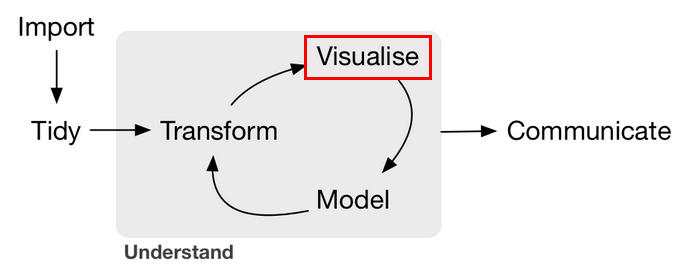
\includegraphics[width=0.75\textwidth]{../img/02_ciclo_4.png}
    \caption{Visualización en el análisis de datos \textcite[Introducción]{grolemund2016r}.}
    \label{fig:ciclo4}
\end{figure}

En \texttt{R} hay muchas maneras de realizar una tarea, esto es
particularmente cierto en lo que se refiere a visualización de datos
\parencite{basevggplot}. A fin de cuentas, lo más importante de la
visualización de datos es cuán útil es esta herramienta para el análisis
de datos y la forma en la que se le indica a la máquina como realizar la
tarea es un elemento importante solo en la medida en la que facilite el
trabajo del estadístico.

Aunque posiblemente cualquiera de los gráficos que se pueden hacer con
\texttt{ggplot2} pueden hacerse también con los gráficos implementados
en el \texttt{base\ graphics} de \texttt{R} \parencite{basevggplot},
aquí se cubre visualización en \texttt{ggplot2} principalmente debido a
que:

\begin{itemize}
\tightlist
\item
  El patrón de programación está definido formalmente mientras que en el
  \texttt{base} no lo está. Esto significa que cuando entiendes cómo
  hacer una gráfica en \texttt{ggplot2}, puedes hacer una gran cantidad
  de gráficos \parencite{basevggplot}.
\item
  \texttt{ggplot2} tiene una gran cantidad de \emph{defaults}
  predefinidos que facilitan realizar gráficos ilustrativos y estéticos
  muy rápidamente \parencite{reasonsggplot}.
\item
  \texttt{ggplot2} es compatible con
  \emph{piping}\footnote{Se introdujo el operador \textit{pipe} de \texttt{R} en la sección de transformación en este capítulo y se mencionó como ayuda en la lectura y escritura de código. Un\textit{pipeline} en programación consiste en un arreglo de elementos de procesamiento en donde la salida de cada elemento es la entrada del siguiente elemento. Este concepto fue concebido por Douglas Mcllroy \parencite{unixpipes}.}
  \parencite{notggplot}.
\item
  Muchas veces, resulta necesario realizar un mismo gráfico para varios
  subconjuntos de datos. Esta tarea se puede hacer en forma directa en
  \texttt{ggplot2} y no en el \texttt{base} a través de facetas.
\end{itemize}

Primero, se cubrirá el concepto detrás de \texttt{ggplot2}, la gramática
de las gráficas. Posteriormente, se describen los componentes de una
gráfica en \texttt{ggplot2}, las capas y sus componentes proporcionando
ejemplos en cada caso.

\subsection{La gramática de las
gráficas}\label{la-gramatica-de-las-graficas}

Es una herramienta que nos permite \parencite{wickham2010layered}:

\begin{itemize}
\tightlist
\item
  Describir los componentes de una gráfica en forma concisa
\item
  Ir más allá de los nombres de la gráfica (e.g.~scatterplot, boxplot,
  etc.)
\item
  Entender la estructura detrás de los gráficos estadísticos
\end{itemize}

\subsection{¿Qué es?}\label{que-es}

La gramática le da reglas al lenguaje y es un sistema formal para
generar enunciados \parencite{wilkinson2006grammar}.
\textcite{wilkinson2006grammar} proporciona una gramática para gráficos
que permite describir y construir una gran cantidad de gráficos
estadísticos. \parencite{wickham2010layered} implementa esta gramática
en el paquete \texttt{ggplot2} de \texttt{R} \parencite{ggplot2}.

La gramática define un gráfico estadístico como un mapeo de datos a
atributos estéticos (un color, una forma) en objetos geométricos
(barras, líneas, puntos). Además, una gráfica puede implicar
transformaciones estadísticas de los datos y se dibuja sobre un sistema
de coordenadas específico. Por último, es posible generar el mismo
gráfico en diferentes subconjuntos de los datos (facetas). La
combinación de estos factores independientes conforman un gráfico
\parencite[][p. 5]{ggplot2}.

La implementación en capas, permite que los usuarios no se limiten
únicamente a los gráficos específicos que se implementan paquete a
paquete sino que puedan realizar tantos gráficos como este lenguaje de
gráficos permita.

\subsection{Base plotting vs.~ggplot}\label{base-plotting-vs.ggplot}

Observemos una gráfica utilizando la base \texttt{diamonds} en donde
graficamos en el eje \(x\) el carataje de diamantes y en el eje \(y\) su
precio:

\begin{Shaded}
\begin{Highlighting}[]
\KeywordTok{data}\NormalTok{(diamonds, }\DataTypeTok{package =} \StringTok{"ggplot2"}\NormalTok{)}
\KeywordTok{str}\NormalTok{(diamonds)}
\end{Highlighting}
\end{Shaded}

\begin{verbatim}
## Classes 'tbl_df', 'tbl' and 'data.frame':    53940 obs. of  10 variables:
##  $ carat  : num  0.23 0.21 0.23 0.29 0.31 0.24 0.24 0.26 0.22 0.23 ...
##  $ cut    : Ord.factor w/ 5 levels "Fair"<"Good"<..: 5 4 2 4 2 3 3 3 1 3 ...
##  $ color  : Ord.factor w/ 7 levels "D"<"E"<"F"<"G"<..: 2 2 2 6 7 7 6 5 2 5 ...
##  $ clarity: Ord.factor w/ 8 levels "I1"<"SI2"<"SI1"<..: 2 3 5 4 2 6 7 3 4 5 ...
##  $ depth  : num  61.5 59.8 56.9 62.4 63.3 62.8 62.3 61.9 65.1 59.4 ...
##  $ table  : num  55 61 65 58 58 57 57 55 61 61 ...
##  $ price  : int  326 326 327 334 335 336 336 337 337 338 ...
##  $ x      : num  3.95 3.89 4.05 4.2 4.34 3.94 3.95 4.07 3.87 4 ...
##  $ y      : num  3.98 3.84 4.07 4.23 4.35 3.96 3.98 4.11 3.78 4.05 ...
##  $ z      : num  2.43 2.31 2.31 2.63 2.75 2.48 2.47 2.53 2.49 2.39 ...
\end{verbatim}

\begin{Shaded}
\begin{Highlighting}[]
\KeywordTok{plot}\NormalTok{(diamonds}\OperatorTok{$}\NormalTok{carat, diamonds}\OperatorTok{$}\NormalTok{price)}
\end{Highlighting}
\end{Shaded}

\includegraphics{ggplot2_files/figure-latex/unnamed-chunk-1-1.pdf}

Ese mismo gráfico, podemos realizarlo con la función \texttt{qplot} del
paquete\texttt{ggplot}:

\begin{Shaded}
\begin{Highlighting}[]
\KeywordTok{qplot}\NormalTok{(}\DataTypeTok{data =}\NormalTok{ diamonds, }\DataTypeTok{x =}\NormalTok{ carat, }\DataTypeTok{y =}\NormalTok{ price, }\DataTypeTok{geom =} \StringTok{"point"}\NormalTok{)}
\end{Highlighting}
\end{Shaded}

\includegraphics{ggplot2_files/figure-latex/unnamed-chunk-2-1.pdf}

En donde especificamos que la variable \texttt{carat} en la base
\texttt{diamonds} mapea al eje \(x\), la variable \texttt{price} en la
misma base al eje \(y\) y queremos que la geometría sea de puntos.

Observa que la estética de la gráfica generada con la función
\texttt{plot} es un poco distinta a la generada con \texttt{qplot}
(función que utiliza \texttt{ggplot}). Verifica la clase que tiene cada
objeto, en el primer caso no tiene y en el segundo tenemos un objeto de
clase \texttt{ggplot} que tiene atributos y que podemos guardar en un
objeto.

\subsection{ggplot}\label{ggplot}

Los componentes de la gramática de gráficas específica para
\texttt{ggplot} son:

\begin{enumerate}
\def\labelenumi{\arabic{enumi}.}
\tightlist
\item
  Una o más capas donde cada cuál tiene:

  \begin{enumerate}
  \def\labelenumii{\alph{enumii}.}
  \tightlist
  \item
    Datos
  \item
    Mapeo estético de los datos (\emph{aesthetic mappings})
  \item
    Un objeto geométrico
  \item
    Una transformación estadística
  \item
    Ajustes en las posiciones de los objetos
  \end{enumerate}
\item
  Una escala para cada estética
\item
  Un sistema de coordenadas
\item
  Una especificación de facetas
\end{enumerate}

Al graficar en \texttt{ggplot} se tiene control sobre todos estos
elementos:

\begin{Shaded}
\begin{Highlighting}[]
\KeywordTok{ggplot}\NormalTok{() }\OperatorTok{+}
\StringTok{  }\KeywordTok{layer}\NormalTok{( }\CommentTok{# una capa}
    \DataTypeTok{data =}\NormalTok{ diamonds, }\CommentTok{# datos}
    \DataTypeTok{mapping =} \KeywordTok{aes}\NormalTok{(}\DataTypeTok{x =}\NormalTok{ carat, }\DataTypeTok{y =}\NormalTok{ price), }\CommentTok{# mapeo estético}
    \DataTypeTok{geom =} \StringTok{"point"}\NormalTok{, }\CommentTok{# geometría}
    \DataTypeTok{stat =} \StringTok{"identity"}\NormalTok{, }\CommentTok{# transformación estadística}
    \DataTypeTok{position =} \StringTok{"identity"} \CommentTok{# ajuste en posición de objetos}
\NormalTok{    ) }\OperatorTok{+}\StringTok{ }
\StringTok{  }\KeywordTok{scale_y_continuous}\NormalTok{() }\OperatorTok{+}\StringTok{ }\CommentTok{# Escala para estética continua en y}
\StringTok{  }\KeywordTok{scale_x_continuous}\NormalTok{() }\OperatorTok{+}\StringTok{ }\CommentTok{# Escala para estética continua en x}
\StringTok{  }\KeywordTok{coord_cartesian}\NormalTok{() }\CommentTok{# Sistema de coordenadas}
\end{Highlighting}
\end{Shaded}

\includegraphics{ggplot2_files/figure-latex/unnamed-chunk-3-1.pdf}

\texttt{ggplot} implementa también una serie de \texttt{defaults}
\parencite[][p. 3]{ggplot2} que facilitan la escritura de nuevas
gráficas pues no es necesario especificar cada uno de los detalles al
agregar una capa. Por tanto, es posible escribir el mismo gráfico
haciendo uso de esos \texttt{defaults}:

\begin{Shaded}
\begin{Highlighting}[]
\KeywordTok{ggplot}\NormalTok{(diamonds, }\KeywordTok{aes}\NormalTok{(carat, price)) }\OperatorTok{+}\StringTok{ }\KeywordTok{geom_point}\NormalTok{()}
\end{Highlighting}
\end{Shaded}

\includegraphics{ggplot2_files/figure-latex/unnamed-chunk-4-1.pdf}

\subsection{Características
importantes}\label{caracteristicas-importantes}

Los componentes de una gráfica son ortogonales:

\begin{verbatim}
- Cambiar uno no debe romper los otros
- Una configuración distinta de componentes es válida
- Puedes construir mayor complejidad agregando capas
\end{verbatim}

\subsection{Las capas}\label{las-capas}

\texttt{ggplot} produce un objeto que se puede convertir en una gráfica.
Es decir, \texttt{R} sabe cómo convertirlo en una gráfica.

Este objeto está formado por capas, mismas que tienen sus entradas
(\emph{inputs}) particulares y que comparten argumentos del gráfico
\texttt{base} generado por la función \texttt{ggplot()}. Con el operador
\texttt{+} se van agregando las distintas capas al mismo objeto.

Así como en otros casos, el objeto en \texttt{R} puede ser guardado en
una variable, se le puede imprimir, se le puede guardar como imagen de
diferentes formatos, o se puede guardar en una lista o en un
\texttt{Rdata}.

\subsection{Componentes de una capa}\label{componentes-de-una-capa}

\subsubsection{Datos y mapa estético}\label{datos-y-mapa-estetico}

Permite mapear las columnas del \texttt{data.frame} de entrada a los
aspectos de la gráfica.

Es decir,

\begin{itemize}
\tightlist
\item
  las coordenadas \(x\), \(y\)
\item
  los grupos (definidos por otra variable)
\item
  el tamaño
\item
  el color
\item
  el relleno
\end{itemize}

Para ejemplificar, generamos una variable \(x\) que proviene de dos
distribuciones normales: mil realizaciones \(N(0, 1)\) y mil
\(N(3, 1)\). Asignamos un grupo a las primeras mil y otro a la segunda.

\begin{Shaded}
\begin{Highlighting}[]
\NormalTok{mix2norm <-}\StringTok{ }\KeywordTok{data.frame}\NormalTok{(}\DataTypeTok{x  =} \KeywordTok{c}\NormalTok{(}\KeywordTok{rnorm}\NormalTok{(}\DecValTok{1000}\NormalTok{), }\KeywordTok{rnorm}\NormalTok{(}\DecValTok{1000}\NormalTok{, }\DecValTok{3}\NormalTok{)), }
                       \DataTypeTok{grupo =} \KeywordTok{as.factor}\NormalTok{(}\KeywordTok{rep}\NormalTok{(}\KeywordTok{c}\NormalTok{(}\DecValTok{1}\NormalTok{,}\DecValTok{2}\NormalTok{),}\DataTypeTok{each=}\DecValTok{1000}\NormalTok{)))}

\KeywordTok{ggplot}\NormalTok{(mix2norm, }\KeywordTok{aes}\NormalTok{(}\DataTypeTok{x=}\NormalTok{x, }\DataTypeTok{color =}\NormalTok{ grupo)) }\OperatorTok{+}\StringTok{ }\KeywordTok{geom_density}\NormalTok{()}
\end{Highlighting}
\end{Shaded}

\includegraphics{ggplot2_files/figure-latex/unnamed-chunk-5-1.pdf}

\subsubsection{Transformaciones
estadísticas}\label{transformaciones-estadisticas}

Ésta puede ser, por ejemplo, un resumen de la entrada (\emph{input})
recibido; se especifica vía el comando \texttt{stat}. Ejemplos:

\begin{itemize}
\tightlist
\item
  binning
\item
  smoothing
\item
  boxplot
\item
  identity
\end{itemize}

Utilizamos, por ejemplo, la transformación \emph{bin}, misma que se
especifica en el objeto geométrico:

\begin{Shaded}
\begin{Highlighting}[]
\KeywordTok{ggplot}\NormalTok{(mix2norm, }\KeywordTok{aes}\NormalTok{(}\DataTypeTok{x=}\NormalTok{x, }\DataTypeTok{color =}\NormalTok{ grupo)) }\OperatorTok{+}\StringTok{ }
\StringTok{  }\KeywordTok{geom_density}\NormalTok{(}\DataTypeTok{stat =} \StringTok{"bin"}\NormalTok{, }\DataTypeTok{binwidth =} \FloatTok{0.1}\NormalTok{)}
\end{Highlighting}
\end{Shaded}

\includegraphics{ggplot2_files/figure-latex/unnamed-chunk-6-1.pdf}

La transformación utilizada tiene asociada parámetros como lo es el
tamaño en el que deben realizarse los colapsos de la variable categórica
(\emph{binwidth}).

\subsubsection{El objeto geométrico}\label{el-objeto-geometrico}

Esto permite especificar el tipo de gráfico a crear. Se especifica con
la \texttt{geom}. Se define de acuerdo a su dimensión, es decir,

\begin{itemize}
\tightlist
\item
  \texttt{0-dim}: puntos, texto
\item
  \texttt{1-dim}: líneas
\item
  \texttt{2-dim}: polígonos, intervalos
\end{itemize}

Otras geometrías incluyen:

\begin{itemize}
\tightlist
\item
  \texttt{geom\_hist}
\item
  \texttt{geom\_bar}
\item
  \texttt{geom\_contour}
\item
  \texttt{geom\_line}
\item
  \texttt{geom\_density}
\end{itemize}

Además, se puede cambiar la transformación estadística manteniendo la
geometría fijada. Al ejemplo anterior, le agregamos una transformación
estadística dentro del objeto geométrico con el parámetro
\texttt{adjust}.

\begin{Shaded}
\begin{Highlighting}[]
\KeywordTok{ggplot}\NormalTok{(mix2norm, }\KeywordTok{aes}\NormalTok{(}\DataTypeTok{x =}\NormalTok{ x, }\DataTypeTok{color =}\NormalTok{ grupo)) }\OperatorTok{+}\StringTok{ }\KeywordTok{geom_density}\NormalTok{(}\DataTypeTok{adjust =} \DecValTok{1}\OperatorTok{/}\DecValTok{2}\NormalTok{)}
\end{Highlighting}
\end{Shaded}

\includegraphics{ggplot2_files/figure-latex/unnamed-chunk-7-1.pdf}

En este caso, estamos pidiendo la mitad del tamaño del bin que se
calcula en forma algorítmica por el paquete.

Viceversa, puede cambiarse la geometría pero mantener la transformación
estadística.

\begin{Shaded}
\begin{Highlighting}[]
\KeywordTok{ggplot}\NormalTok{(mix2norm, }\KeywordTok{aes}\NormalTok{(}\DataTypeTok{x =}\NormalTok{ x, }\DataTypeTok{color =}\NormalTok{ grupo)) }\OperatorTok{+}\StringTok{ }\KeywordTok{stat_density}\NormalTok{(}\DataTypeTok{adjust =} \DecValTok{1}\OperatorTok{/}\DecValTok{2}\NormalTok{)}
\end{Highlighting}
\end{Shaded}

\includegraphics{ggplot2_files/figure-latex/unnamed-chunk-8-1.pdf}

Revisa el comando \texttt{position} y \texttt{geometry}. Revisa sus
defaults y copia algunos de los ejemplos en la documentación.

\texttt{geom\_density} por ejemplo utiliza \texttt{ribbon} o una cosa
que a veces encontrarán en español como violín.

\renewcommand\bcStyleTitre[1]{\large\textcolor{bbblack}{#1}}

\begin{bclogo}[
  couleur=llred,
  arrondi=0,
  logo=\bcstop,
  barre=none,
  noborder=true]{Ejercicios}
\begin{enumerate}
\item Genera una gráfica con la función \texttt{ggplot} en donde los datos sea
la base \texttt{diamonds} y la estética sea $x = price$. Especifica como geometría
una densidad.
\item Cambia el color y el relleno de la geometría a gris (\texttt{grey50})
\item Cambia la geometría a \texttt{ribbon}, cambia los parámetros necesarios
para que funcione.
\item Agrega una faceta para que se haga un gráfico para cada uno de los subconjuntos
definidos por la variable \texttt{cut}.
\item Agrega a la gráfica el comando \texttt{coord\_flip} para que el precio este
en el eje $y$.
\end{enumerate}

\end{bclogo}

\begin{Shaded}
\begin{Highlighting}[]
\CommentTok{# Respuestas}
\CommentTok{# 1}
\NormalTok{g <-}\StringTok{ }\KeywordTok{ggplot}\NormalTok{(diamonds, }\KeywordTok{aes}\NormalTok{(}\DataTypeTok{x =}\NormalTok{ price)) }\OperatorTok{+}\StringTok{ }\KeywordTok{stat_density}\NormalTok{()}
\NormalTok{g}
\CommentTok{# 2}
\NormalTok{g }\OperatorTok{+}
\StringTok{  }\KeywordTok{stat_density}\NormalTok{(}\DataTypeTok{fill =} \StringTok{"grey50"}\NormalTok{, }\DataTypeTok{colour =} \StringTok{"grey50"}\NormalTok{) }
\CommentTok{# 3}
\NormalTok{g <-}\StringTok{ }\NormalTok{g }\OperatorTok{+}
\StringTok{  }\KeywordTok{stat_density}\NormalTok{(}\KeywordTok{aes}\NormalTok{(}\DataTypeTok{ymax =}\NormalTok{ ..density..,  }\DataTypeTok{ymin =} \OperatorTok{-}\NormalTok{..density..),}
    \DataTypeTok{fill =} \StringTok{"grey50"}\NormalTok{, }\DataTypeTok{colour =} \StringTok{"grey50"}\NormalTok{,}
    \DataTypeTok{geom =} \StringTok{"ribbon"}\NormalTok{, }\DataTypeTok{position =} \StringTok{"identity"}\NormalTok{)}
\NormalTok{g}
\CommentTok{# 4}
\NormalTok{g <-}\StringTok{ }\NormalTok{g  }\OperatorTok{+}
\StringTok{  }\KeywordTok{facet_grid}\NormalTok{(. }\OperatorTok{~}\StringTok{ }\NormalTok{cut) }
\NormalTok{g}
\CommentTok{# 5}
\NormalTok{g }\OperatorTok{+}\StringTok{ }\KeywordTok{coord_flip}\NormalTok{()}
\end{Highlighting}
\end{Shaded}

\subsubsection{Posición}\label{posicion}

Es posible especificar la posición de cada una de las capas en relación
a otras. Ejemplos:

\begin{itemize}
\tightlist
\item
  \texttt{dodge}
\item
  \texttt{identity}
\item
  \texttt{jitter}
\end{itemize}

\begin{Shaded}
\begin{Highlighting}[]
\KeywordTok{ggplot}\NormalTok{(mix2norm, }\KeywordTok{aes}\NormalTok{(}\DataTypeTok{x=}\NormalTok{x, }\DataTypeTok{color =}\NormalTok{ grupo)) }\OperatorTok{+}\StringTok{ }
\StringTok{  }\KeywordTok{stat_density}\NormalTok{(}\DataTypeTok{adjust=}\DecValTok{1}\OperatorTok{/}\DecValTok{2}\NormalTok{, }\DataTypeTok{size=}\DecValTok{2}\NormalTok{, }\DataTypeTok{position =} \StringTok{"identity"}\NormalTok{, }\DataTypeTok{geom =} \StringTok{"line"}\NormalTok{)}
\end{Highlighting}
\end{Shaded}

\includegraphics{ggplot2_files/figure-latex/unnamed-chunk-10-1.pdf}

\subsubsection{Escalas}\label{escalas}

Determina cuál valor de entrada mapea a qué estética específica. Se
escribe usando \texttt{scale}. Hay de todo:

\begin{itemize}
\tightlist
\item
  \texttt{continous}
\item
  \texttt{logarithmic}
\item
  \texttt{values\ to\ shapes}
\item
  \texttt{what\ limits}
\item
  \texttt{what\ labels}
\item
  \texttt{what\ marks}
\end{itemize}

\begin{Shaded}
\begin{Highlighting}[]
\KeywordTok{ggplot}\NormalTok{(mix2norm, }\KeywordTok{aes}\NormalTok{(}\DataTypeTok{x=}\NormalTok{x, }\DataTypeTok{color =}\NormalTok{ grupo)) }\OperatorTok{+}\StringTok{ }
\StringTok{  }\KeywordTok{stat_density}\NormalTok{(}\DataTypeTok{adjust=}\DecValTok{1}\OperatorTok{/}\DecValTok{2}\NormalTok{, }\DataTypeTok{size=}\DecValTok{2}\NormalTok{, }\DataTypeTok{position =}\StringTok{"identity"}\NormalTok{, }\DataTypeTok{geom =}\StringTok{"line"}\NormalTok{) }\OperatorTok{+}
\StringTok{  }\KeywordTok{scale_y_log10}\NormalTok{(}\DataTypeTok{limits =} \KeywordTok{c}\NormalTok{(}\FloatTok{1e-5}\NormalTok{,}\DecValTok{1}\NormalTok{))}
\end{Highlighting}
\end{Shaded}

\includegraphics{ggplot2_files/figure-latex/unnamed-chunk-11-1.pdf}

\subsubsection{Coordenadas}\label{coordenadas}

Te permite especificar las posiciones de las cosas y cómo mapean a las
posiciones en la pantalla. Antes todo era entorno a cómo le dices las
cosas a \texttt{R} pero también importa cómo las ves. Coordenadas
distintas pueden afectar a los objetos geométricos. Ejemplos:

\begin{itemize}
\tightlist
\item
  \texttt{cartesian}
\item
  \texttt{polar}
\item
  \texttt{map-projection}
\end{itemize}

\begin{Shaded}
\begin{Highlighting}[]
\KeywordTok{ggplot}\NormalTok{(mix2norm, }\KeywordTok{aes}\NormalTok{(}\DataTypeTok{x =}\NormalTok{ x, }\DataTypeTok{color =}\NormalTok{ grupo)) }\OperatorTok{+}\StringTok{ }
\StringTok{  }\KeywordTok{stat_density}\NormalTok{(}\DataTypeTok{adjust =} \DecValTok{1}\OperatorTok{/}\DecValTok{2}\NormalTok{, }\DataTypeTok{size =} \DecValTok{2}\NormalTok{, }\DataTypeTok{position =} \StringTok{"identity"}\NormalTok{, }\DataTypeTok{geom =} \StringTok{"line"}\NormalTok{) }\OperatorTok{+}
\StringTok{  }\KeywordTok{coord_polar}\NormalTok{()}
\end{Highlighting}
\end{Shaded}

\includegraphics{ggplot2_files/figure-latex/unnamed-chunk-12-1.pdf}

\subsubsection{Facetas}\label{facetas}

Permite arreglar diferentes gráficas en un grid o panel.

\begin{Shaded}
\begin{Highlighting}[]
\KeywordTok{ggplot}\NormalTok{(mix2norm, }\KeywordTok{aes}\NormalTok{(}\DataTypeTok{x =}\NormalTok{ x, }\DataTypeTok{color =}\NormalTok{ grupo)) }\OperatorTok{+}\StringTok{ }
\StringTok{  }\KeywordTok{stat_density}\NormalTok{(}\DataTypeTok{adjust =} \DecValTok{1}\OperatorTok{/}\DecValTok{2}\NormalTok{, }\DataTypeTok{size =} \DecValTok{2}\NormalTok{, }\DataTypeTok{position =} \StringTok{"identity"}\NormalTok{, }\DataTypeTok{geom =} \StringTok{"line"}\NormalTok{) }\OperatorTok{+}
\StringTok{  }\KeywordTok{facet_grid}\NormalTok{(grupo }\OperatorTok{~}\StringTok{ }\NormalTok{.)}
\end{Highlighting}
\end{Shaded}

\includegraphics{ggplot2_files/figure-latex/unnamed-chunk-13-1.pdf}

Ve el help de \texttt{facet\_wrap}

\section{Material adicional}\label{material-adicional}

\begin{itemize}
\tightlist
\item
  Importación

  \begin{itemize}
  \tightlist
  \item
    Curso \textbf{Importing Data in R (Part 1)} de
    \href{https://www.datacamp.com/courses/importing-data-in-r-part-1}{Data
    Camp}.
  \item
    Curso \textbf{Importing Data in R (Part 2)} de
    \href{https://www.datacamp.com/courses/importing-data-in-r-part-2}{Data
    Camp}.
  \end{itemize}
\item
  \texttt{dplyr} y \texttt{tidyr}

  \begin{itemize}
  \tightlist
  \item
    Curso de \texttt{swirl} \textbf{Getting and cleaning data}.
  \item
    Curso \textbf{Cleaning Data in R} de
    \href{https://www.datacamp.com/courses/cleaning-data-in-r}{Data
    Camp}.
  \item
    Curso \textbf{Data Manipulation in R with dplyr} de
    \href{https://www.datacamp.com/courses/dplyr-data-manipulation-r-tutorial}{Data
    Camp}.
  \item
    Curso \textbf{Joining data in R with dplyr} de
    \href{https://www.datacamp.com/courses/joining-data-in-r-with-dplyr}{Data
    Camp}.
  \end{itemize}
\item
  Gráficos del \texttt{base}

  \begin{itemize}
  \tightlist
  \item
    Curso de \texttt{swirl} \textbf{Overview of Statistics}.
  \end{itemize}
\item
  \texttt{ggplot2}

  \begin{itemize}
  \tightlist
  \item
    Curso de \texttt{swirl} \textbf{Exploratory data analysis}.
  \item
    Curso \textbf{Data Visualization in R} de
    \href{https://www.datacamp.com/courses/data-visualization-in-r}{Data
    Camp}.
  \item
    Curso \textbf{Data Visualization with ggplot2 (Part 1)} de
    \href{https://www.datacamp.com/courses/data-visualization-with-ggplot2-1}{Data
    Camp}.
  \item
    Curso \textbf{Data Visualization with ggplot2 (Part 2)} de
    \href{https://www.datacamp.com/courses/data-visualization-with-ggplot2-2}{Data
    Camp}.
  \item
    Curso \textbf{Data Visualization with ggplot2 (Part 3)} de
    \href{https://www.datacamp.com/courses/data-visualization-with-ggplot2-3}{Data
    Camp}.
  \end{itemize}
\end{itemize}


\end{document}


\addtocontents{toc}{\vspace{2em}} % Add a gap in the Contents, for aesthetics

\appendix % Cue to tell LaTeX that the following 'chapters' are Appendices
\graphicspath{{00_otros/}}
\chapter{Markdown}\label{apendice-markdown}
\documentclass[]{article}
\usepackage{lmodern}
\usepackage{amssymb,amsmath}
\usepackage{ifxetex,ifluatex}
\usepackage{fixltx2e} % provides \textsubscript
\ifnum 0\ifxetex 1\fi\ifluatex 1\fi=0 % if pdftex
  \usepackage[T1]{fontenc}
  \usepackage[utf8]{inputenc}
\else % if luatex or xelatex
  \ifxetex
    \usepackage{mathspec}
  \else
    \usepackage{fontspec}
  \fi
  \defaultfontfeatures{Ligatures=TeX,Scale=MatchLowercase}
\fi
% use upquote if available, for straight quotes in verbatim environments
\IfFileExists{upquote.sty}{\usepackage{upquote}}{}
% use microtype if available
\IfFileExists{microtype.sty}{%
\usepackage{microtype}
\UseMicrotypeSet[protrusion]{basicmath} % disable protrusion for tt fonts
}{}
\usepackage[margin=1in]{geometry}
\usepackage{hyperref}
\hypersetup{unicode=true,
            pdftitle={Markdown},
            pdfborder={0 0 0},
            breaklinks=true}
\urlstyle{same}  % don't use monospace font for urls
\usepackage{color}
\usepackage{fancyvrb}
\newcommand{\VerbBar}{|}
\newcommand{\VERB}{\Verb[commandchars=\\\{\}]}
\DefineVerbatimEnvironment{Highlighting}{Verbatim}{commandchars=\\\{\}}
% Add ',fontsize=\small' for more characters per line
\usepackage{framed}
\definecolor{shadecolor}{RGB}{248,248,248}
\newenvironment{Shaded}{\begin{snugshade}}{\end{snugshade}}
\newcommand{\KeywordTok}[1]{\textcolor[rgb]{0.13,0.29,0.53}{\textbf{#1}}}
\newcommand{\DataTypeTok}[1]{\textcolor[rgb]{0.13,0.29,0.53}{#1}}
\newcommand{\DecValTok}[1]{\textcolor[rgb]{0.00,0.00,0.81}{#1}}
\newcommand{\BaseNTok}[1]{\textcolor[rgb]{0.00,0.00,0.81}{#1}}
\newcommand{\FloatTok}[1]{\textcolor[rgb]{0.00,0.00,0.81}{#1}}
\newcommand{\ConstantTok}[1]{\textcolor[rgb]{0.00,0.00,0.00}{#1}}
\newcommand{\CharTok}[1]{\textcolor[rgb]{0.31,0.60,0.02}{#1}}
\newcommand{\SpecialCharTok}[1]{\textcolor[rgb]{0.00,0.00,0.00}{#1}}
\newcommand{\StringTok}[1]{\textcolor[rgb]{0.31,0.60,0.02}{#1}}
\newcommand{\VerbatimStringTok}[1]{\textcolor[rgb]{0.31,0.60,0.02}{#1}}
\newcommand{\SpecialStringTok}[1]{\textcolor[rgb]{0.31,0.60,0.02}{#1}}
\newcommand{\ImportTok}[1]{#1}
\newcommand{\CommentTok}[1]{\textcolor[rgb]{0.56,0.35,0.01}{\textit{#1}}}
\newcommand{\DocumentationTok}[1]{\textcolor[rgb]{0.56,0.35,0.01}{\textbf{\textit{#1}}}}
\newcommand{\AnnotationTok}[1]{\textcolor[rgb]{0.56,0.35,0.01}{\textbf{\textit{#1}}}}
\newcommand{\CommentVarTok}[1]{\textcolor[rgb]{0.56,0.35,0.01}{\textbf{\textit{#1}}}}
\newcommand{\OtherTok}[1]{\textcolor[rgb]{0.56,0.35,0.01}{#1}}
\newcommand{\FunctionTok}[1]{\textcolor[rgb]{0.00,0.00,0.00}{#1}}
\newcommand{\VariableTok}[1]{\textcolor[rgb]{0.00,0.00,0.00}{#1}}
\newcommand{\ControlFlowTok}[1]{\textcolor[rgb]{0.13,0.29,0.53}{\textbf{#1}}}
\newcommand{\OperatorTok}[1]{\textcolor[rgb]{0.81,0.36,0.00}{\textbf{#1}}}
\newcommand{\BuiltInTok}[1]{#1}
\newcommand{\ExtensionTok}[1]{#1}
\newcommand{\PreprocessorTok}[1]{\textcolor[rgb]{0.56,0.35,0.01}{\textit{#1}}}
\newcommand{\AttributeTok}[1]{\textcolor[rgb]{0.77,0.63,0.00}{#1}}
\newcommand{\RegionMarkerTok}[1]{#1}
\newcommand{\InformationTok}[1]{\textcolor[rgb]{0.56,0.35,0.01}{\textbf{\textit{#1}}}}
\newcommand{\WarningTok}[1]{\textcolor[rgb]{0.56,0.35,0.01}{\textbf{\textit{#1}}}}
\newcommand{\AlertTok}[1]{\textcolor[rgb]{0.94,0.16,0.16}{#1}}
\newcommand{\ErrorTok}[1]{\textcolor[rgb]{0.64,0.00,0.00}{\textbf{#1}}}
\newcommand{\NormalTok}[1]{#1}
\usepackage{longtable,booktabs}
\usepackage{graphicx,grffile}
\makeatletter
\def\maxwidth{\ifdim\Gin@nat@width>\linewidth\linewidth\else\Gin@nat@width\fi}
\def\maxheight{\ifdim\Gin@nat@height>\textheight\textheight\else\Gin@nat@height\fi}
\makeatother
% Scale images if necessary, so that they will not overflow the page
% margins by default, and it is still possible to overwrite the defaults
% using explicit options in \includegraphics[width, height, ...]{}
\setkeys{Gin}{width=\maxwidth,height=\maxheight,keepaspectratio}
\usepackage[normalem]{ulem}
% avoid problems with \sout in headers with hyperref:
\pdfstringdefDisableCommands{\renewcommand{\sout}{}}
\IfFileExists{parskip.sty}{%
\usepackage{parskip}
}{% else
\setlength{\parindent}{0pt}
\setlength{\parskip}{6pt plus 2pt minus 1pt}
}
\setlength{\emergencystretch}{3em}  % prevent overfull lines
\providecommand{\tightlist}{%
  \setlength{\itemsep}{0pt}\setlength{\parskip}{0pt}}
\setcounter{secnumdepth}{0}
% Redefines (sub)paragraphs to behave more like sections
\ifx\paragraph\undefined\else
\let\oldparagraph\paragraph
\renewcommand{\paragraph}[1]{\oldparagraph{#1}\mbox{}}
\fi
\ifx\subparagraph\undefined\else
\let\oldsubparagraph\subparagraph
\renewcommand{\subparagraph}[1]{\oldsubparagraph{#1}\mbox{}}
\fi

%%% Use protect on footnotes to avoid problems with footnotes in titles
\let\rmarkdownfootnote\footnote%
\def\footnote{\protect\rmarkdownfootnote}

%%% Change title format to be more compact
\usepackage{titling}

% Create subtitle command for use in maketitle
\newcommand{\subtitle}[1]{
  \posttitle{
    \begin{center}\large#1\end{center}
    }
}

\setlength{\droptitle}{-2em}
  \title{Markdown}
  \pretitle{\vspace{\droptitle}\centering\huge}
  \posttitle{\par}
  \author{}
  \preauthor{}\postauthor{}
  \date{}
  \predate{}\postdate{}

\usepackage[
  backend=biber,
  style=alphabetic,
  sorting=ynt,
  citestyle=authoryear
  ]{biblatex}
\addbibresource{../lit/bib.bib}

\usepackage[utf8]{inputenc}
\usepackage[spanish]{babel}

%%%% Frames
\ifxetex
    \makeatletter % undo the wrong changes made by mathspec
    \let\RequirePackage\original@RequirePackage
    \let\usepackage\RequirePackage
    \makeatother
\fi

\usepackage{xcolor}
\usepackage[tikz]{bclogo}
\usepackage[framemethod=tikz]{mdframed}
\usepackage{lipsum}
\usepackage[many]{tcolorbox}

\definecolor{bgblue}{RGB}{245,243,253}
\definecolor{ttblue}{RGB}{91,194,224}
\definecolor{llred}{RGB}{255,228,225}
\definecolor{bbblack}{RGB}{0,0,0}

\mdfdefinestyle{mystyle}{%
  rightline=true,
  innerleftmargin=10,
  innerrightmargin=10,
  outerlinewidth=3pt,
  topline=false,
  rightline=true,
  bottomline=false,
  skipabove=\topsep,
  skipbelow=\topsep
}

\newtcolorbox{curiosidad}[1][]{
  breakable,
  title=#1,
  colback=white,
  colbacktitle=white,
  coltitle=black,
  fonttitle=\bfseries,
  bottomrule=0pt,
  toprule=0pt,
  leftrule=3pt,
  rightrule=3pt,
  titlerule=0pt,
  arc=0pt,
  outer arc=0pt,
  colframe=black,
}

\newtcolorbox{nota}[1][]{
  breakable,
  freelance,
  title=#1,
  colback=white,
  colbacktitle=white,
  coltitle=black,
  fonttitle=\bfseries,
  bottomrule=0pt,
  boxrule=0pt,
  colframe=white,
  overlay unbroken and first={
  \draw[red!75!black,line width=3pt]
    ([xshift=5pt]frame.north west) -- 
    (frame.north west) -- 
    (frame.south west);
  \draw[red!75!black,line width=3pt]
    ([xshift=-5pt]frame.north east) -- 
    (frame.north east) -- 
    (frame.south east);
  },
  overlay unbroken app={
  \draw[red!75!black,line width=3pt,line cap=rect]
    (frame.south west) -- 
    ([xshift=5pt]frame.south west);
  \draw[red!75!black,line width=3pt,line cap=rect]
    (frame.south east) -- 
    ([xshift=-5pt]frame.south east);
  },
  overlay middle and last={
  \draw[red!75!black,line width=3pt]
    (frame.north west) -- 
    (frame.south west);
  \draw[red!75!black,line width=3pt]
    (frame.north east) -- 
    (frame.south east);
  },
  overlay last app={
  \draw[red!75!black,line width=3pt,line cap=rect]
    (frame.south west) --
    ([xshift=5pt]frame.south west);
  \draw[red!75!black,line width=3pt,line cap=rect]
    (frame.south east) --
    ([xshift=-5pt]frame.south east);
  },
}

\begin{document}


Estamos acostumbrados a editores del tipo \emph{what you see is what you
get}. \texttt{Markdown} permite escribir contenidos en \textbf{texto
plano} con una sintáxis para darle formato. Sobre esta sintáxis la
herramienta de software en Perl convierte el texto plano a HTML
\parencite{markdown}.

Tiene un alfabeto y símbolos que, una vez procesados, se ven de cierta
forma. A diferencia de un editor como Word en el que la versión de cada
computadora cambia la manera en la que se ven los documentos, con
\texttt{Markdown} esto no sucede.

Este lenguaje se está volviendo cada vez más común y, en particular,
páginas como GitHub y reddit lo utilizan para sus comentarios.

La curva de aprendizaje es mínima. En lo que se va memorizando el
alfabeto de markdown, lo más útil es tener una lista de fácil acceso con
los caracteres más comúnes y lo que hacen. A continuación, se
proporciona un listado de la sintáxis más común
\footnote{Basado en \textcite{markdowncheet1} y en \textcite{markdowncheet2}.}.

\subsection{Encabezados}\label{encabezados}

\begin{verbatim}
# Nivel 1
## Nivel 2
### Nivel 3
#### Nivel 4

... y asi
\end{verbatim}

\section{Nivel 1}\label{nivel-1}

\subsection{Nivel 2}\label{nivel-2}

\subsubsection{Nivel 3}\label{nivel-3}

\paragraph{Nivel 4}\label{nivel-4}

\section{Lineas horizontales}\label{lineas-horizontales}

Con tres o mas de los siguientes

\begin{verbatim}
---

Guiones

***
Asteriscos

___

Guiones bajos
\end{verbatim}

\begin{center}\rule{0.5\linewidth}{\linethickness}\end{center}

Guiones

\begin{center}\rule{0.5\linewidth}{\linethickness}\end{center}

Asteriscos

\begin{center}\rule{0.5\linewidth}{\linethickness}\end{center}

Guiones bajos

\section{Énfasis}\label{enfasis}

\begin{verbatim}
*italica* o _italica_
**negritas** o __negritas__
**_combinado_**
**Uno en negritas _el otro combinado_**
~~tachar~~
\end{verbatim}

\begin{itemize}
\tightlist
\item
  \emph{italica} o \emph{italica}
\item
  \textbf{negritas} o \textbf{negritas}
\item
  \textbf{\emph{combinado}}
\item
  \textbf{Uno en negritas \emph{el otro combinado}}
\item
  \sout{tachar}
\end{itemize}

\section{Bloques}\label{bloques}

\begin{verbatim}
> Ejemplo: Un bloque de varias
> lineas.
\end{verbatim}

\begin{quote}
Ejemplo: Un bloque de varias líneas.
\end{quote}

\section{Listas}\label{listas}

\begin{verbatim}
1. Primero
2. Segundo
    - Primer elemento del segundo
    - Segundo elemento del segundo
7. No tengo que cambiar el nombre, se pondra el correcto
    i. Una sublista con incisos
    ii. Mas incisos
4. Mas cosas
    a. Otra cosa
    b. Una mas
5. Otra manera de hacer listas no ordenadas
    * Usando asteriscos
    - O usando menos
    - O usando el signo de mas
\end{verbatim}

\begin{enumerate}
\def\labelenumi{\arabic{enumi}.}
\tightlist
\item
  Primero
\item
  Segundo

  \begin{itemize}
  \tightlist
  \item
    Primer elemento del segundo
  \item
    Segundo elemento del segundo
  \end{itemize}
\item
  No tengo que cambiar el nombre, se pondrá el correcto

  \begin{enumerate}
  \def\labelenumii{\roman{enumii}.}
  \tightlist
  \item
    Una sublista con incisos
  \item
    Mas incisos
  \end{enumerate}
\item
  Mas cosas

  \begin{enumerate}
  \def\labelenumii{\alph{enumii}.}
  \tightlist
  \item
    Otra cosa
  \item
    Una mas
  \end{enumerate}
\item
  Otra manera de hacer listas no ordenadas

  \begin{itemize}
  \tightlist
  \item
    Usando asteriscos
  \item
    O usando menos
  \item
    O usando el signo de mas
  \end{itemize}
\end{enumerate}

\section{Links}\label{links}

\begin{verbatim}
[Esto es lo que se ve](https://www.google.com)
[Esto es lo que se ve y el mensaje "Google" aparece en el hover]
(https://www.google.com "Google")
[Puedo hacer referencia a un archivo local](readme.md)
[Puedes poner referencias][1]

Detecata urls completos www.google.com o google.com

Y luego pones a donde te lleva la referencia
[1]: https://en.wikipedia.org/wiki/42_%28number%29#The_Hitchhiker.27s_Guide_to_the_Galaxy



\end{verbatim}

\href{https://www.google.com}{Esto es lo que se ve}

\href{https://www.google.com}{Esto es lo que se ve y el mensaje
``Google'' aparece en el hover}

\href{readme.md}{Puedo hacer referencia a un archivo local}

\href{https://en.wikipedia.org/wiki/42_\%28number\%29\#The_Hitchhiker.27s_Guide_to_the_Galaxy}{Puedes
poner referencias con numeros}

Luego quieres hacer referencias a otra parte del documento
\href{http://www.reddit.com}{por lo tanto, puedes ligar texto}

Detecta urls completos \url{http://www.google.com}

Y luego pones a dónde te lleva la referencia

Nota que los espacios entre lineas son importantes.

\section{Imágenes}\label{imagenes}

\begin{verbatim}
Puedes ponerlo en una misma linea: 
![alt text](dw.png "Es lo mejor")

Reference-style: 
![alt text][logo]

[logo]: dw.png "Sin duda alguna"
\end{verbatim}

Puedes ponerlo en una misma linea: 
\includegraphics{dw.png}

Reference-style: 
\includegraphics{dw.png}

\section{Tablas}\label{tablas}

\begin{verbatim}
Una tabla simple 

Encabezado 1  | Encabezado dos
------------- | --------------
Contenido     | Contenido
Contenido     | Contenido 
\end{verbatim}

\begin{longtable}[]{@{}ll@{}}
\toprule
Encabezado 1 & Encabezado dos\tabularnewline
\midrule
\endhead
Contenido & Contenido\tabularnewline
Contenido & Contenido\tabularnewline
\bottomrule
\end{longtable}

\begin{verbatim}
Una tabla alineada. La alineacion la puedes hacer por columnas

| Derecha | Centro | Iquierda |
| ----: | :----: | :---- |
| 10    | 10     | 10    |
| 1000  | 1000   | 1000  |
\end{verbatim}

\begin{longtable}[]{@{}rcl@{}}
\toprule
Derecha & Centro & Izquierda\tabularnewline
\midrule
\endhead
10 & 10 & 10\tabularnewline
1000 & 1000 & 1000\tabularnewline
\bottomrule
\end{longtable}

\section{HTML}\label{html}

Si sabes html, puedes utilizarlo directo.

\begin{verbatim}
<dl>
  <dt>Lista de definiciones</dt>
  <dd> Una def.</dd>

  <dt>Markdown en HTML</dt>
  <dd>No *siempre* funciona **bien**. Puro HTML <em>para que funcione</em>.</dd>
</dl>

Puedes controlar mejor las imagenes

<img src="img/imagen.png" align="middle" height="50" width="75" margin="0 auto" />
\end{verbatim}

Lista de definiciones

Una def.

Markdown en HTML

No \emph{siempre} funciona muy \textbf{bien}. Usa puro HTML para que
funcione siempre.

Puedes controlar mejor las imágenes

\section{Código}\label{codigo}

\begin{verbatim}
En una linea puedo poner `código`
\end{verbatim}

En una linea puedo poner \texttt{código}.

Para poner bloques de código se utilizan tres acentos invertidos y se
especifica el lenguaje.

\begin{Shaded}
\begin{Highlighting}[]
\ImportTok{import}\NormalTok{ requests}
\BuiltInTok{print} \StringTok{"¡Hola mundo!"}
\end{Highlighting}
\end{Shaded}

\begin{Shaded}
\begin{Highlighting}[]
\KeywordTok{select}\NormalTok{ * }\KeywordTok{from}\NormalTok{ tabla;}
\end{Highlighting}
\end{Shaded}

\begin{Shaded}
\begin{Highlighting}[]
\KeywordTok{library}\NormalTok{(dplyr)}
\end{Highlighting}
\end{Shaded}

\begin{verbatim}
Sin lenguaje, no lo resalta
\end{verbatim}

\section{Párrafos}\label{parrafos}

\begin{verbatim}
Si
escribo asi
me lo junta todo.

Debo separar para iniciar otro parrafo.
\end{verbatim}

Si escribo así me lo junta todo.

Debo separar para iniciar otro párrafo.


\end{document}


\chapter{Packrat}\label{apendice-packrat}
\documentclass[]{article}
\usepackage{lmodern}
\usepackage{amssymb,amsmath}
\usepackage{ifxetex,ifluatex}
\usepackage{fixltx2e} % provides \textsubscript
\ifnum 0\ifxetex 1\fi\ifluatex 1\fi=0 % if pdftex
  \usepackage[T1]{fontenc}
  \usepackage[utf8]{inputenc}
\else % if luatex or xelatex
  \ifxetex
    \usepackage{mathspec}
  \else
    \usepackage{fontspec}
  \fi
  \defaultfontfeatures{Ligatures=TeX,Scale=MatchLowercase}
\fi
% use upquote if available, for straight quotes in verbatim environments
\IfFileExists{upquote.sty}{\usepackage{upquote}}{}
% use microtype if available
\IfFileExists{microtype.sty}{%
\usepackage{microtype}
\UseMicrotypeSet[protrusion]{basicmath} % disable protrusion for tt fonts
}{}
\usepackage[margin=1in]{geometry}
\usepackage{hyperref}
\hypersetup{unicode=true,
            pdftitle={Packrat},
            pdfborder={0 0 0},
            breaklinks=true}
\urlstyle{same}  % don't use monospace font for urls
\usepackage{color}
\usepackage{fancyvrb}
\newcommand{\VerbBar}{|}
\newcommand{\VERB}{\Verb[commandchars=\\\{\}]}
\DefineVerbatimEnvironment{Highlighting}{Verbatim}{commandchars=\\\{\}}
% Add ',fontsize=\small' for more characters per line
\usepackage{framed}
\definecolor{shadecolor}{RGB}{248,248,248}
\newenvironment{Shaded}{\begin{snugshade}}{\end{snugshade}}
\newcommand{\KeywordTok}[1]{\textcolor[rgb]{0.13,0.29,0.53}{\textbf{#1}}}
\newcommand{\DataTypeTok}[1]{\textcolor[rgb]{0.13,0.29,0.53}{#1}}
\newcommand{\DecValTok}[1]{\textcolor[rgb]{0.00,0.00,0.81}{#1}}
\newcommand{\BaseNTok}[1]{\textcolor[rgb]{0.00,0.00,0.81}{#1}}
\newcommand{\FloatTok}[1]{\textcolor[rgb]{0.00,0.00,0.81}{#1}}
\newcommand{\ConstantTok}[1]{\textcolor[rgb]{0.00,0.00,0.00}{#1}}
\newcommand{\CharTok}[1]{\textcolor[rgb]{0.31,0.60,0.02}{#1}}
\newcommand{\SpecialCharTok}[1]{\textcolor[rgb]{0.00,0.00,0.00}{#1}}
\newcommand{\StringTok}[1]{\textcolor[rgb]{0.31,0.60,0.02}{#1}}
\newcommand{\VerbatimStringTok}[1]{\textcolor[rgb]{0.31,0.60,0.02}{#1}}
\newcommand{\SpecialStringTok}[1]{\textcolor[rgb]{0.31,0.60,0.02}{#1}}
\newcommand{\ImportTok}[1]{#1}
\newcommand{\CommentTok}[1]{\textcolor[rgb]{0.56,0.35,0.01}{\textit{#1}}}
\newcommand{\DocumentationTok}[1]{\textcolor[rgb]{0.56,0.35,0.01}{\textbf{\textit{#1}}}}
\newcommand{\AnnotationTok}[1]{\textcolor[rgb]{0.56,0.35,0.01}{\textbf{\textit{#1}}}}
\newcommand{\CommentVarTok}[1]{\textcolor[rgb]{0.56,0.35,0.01}{\textbf{\textit{#1}}}}
\newcommand{\OtherTok}[1]{\textcolor[rgb]{0.56,0.35,0.01}{#1}}
\newcommand{\FunctionTok}[1]{\textcolor[rgb]{0.00,0.00,0.00}{#1}}
\newcommand{\VariableTok}[1]{\textcolor[rgb]{0.00,0.00,0.00}{#1}}
\newcommand{\ControlFlowTok}[1]{\textcolor[rgb]{0.13,0.29,0.53}{\textbf{#1}}}
\newcommand{\OperatorTok}[1]{\textcolor[rgb]{0.81,0.36,0.00}{\textbf{#1}}}
\newcommand{\BuiltInTok}[1]{#1}
\newcommand{\ExtensionTok}[1]{#1}
\newcommand{\PreprocessorTok}[1]{\textcolor[rgb]{0.56,0.35,0.01}{\textit{#1}}}
\newcommand{\AttributeTok}[1]{\textcolor[rgb]{0.77,0.63,0.00}{#1}}
\newcommand{\RegionMarkerTok}[1]{#1}
\newcommand{\InformationTok}[1]{\textcolor[rgb]{0.56,0.35,0.01}{\textbf{\textit{#1}}}}
\newcommand{\WarningTok}[1]{\textcolor[rgb]{0.56,0.35,0.01}{\textbf{\textit{#1}}}}
\newcommand{\AlertTok}[1]{\textcolor[rgb]{0.94,0.16,0.16}{#1}}
\newcommand{\ErrorTok}[1]{\textcolor[rgb]{0.64,0.00,0.00}{\textbf{#1}}}
\newcommand{\NormalTok}[1]{#1}
\usepackage{graphicx,grffile}
\makeatletter
\def\maxwidth{\ifdim\Gin@nat@width>\linewidth\linewidth\else\Gin@nat@width\fi}
\def\maxheight{\ifdim\Gin@nat@height>\textheight\textheight\else\Gin@nat@height\fi}
\makeatother
% Scale images if necessary, so that they will not overflow the page
% margins by default, and it is still possible to overwrite the defaults
% using explicit options in \includegraphics[width, height, ...]{}
\setkeys{Gin}{width=\maxwidth,height=\maxheight,keepaspectratio}
\IfFileExists{parskip.sty}{%
\usepackage{parskip}
}{% else
\setlength{\parindent}{0pt}
\setlength{\parskip}{6pt plus 2pt minus 1pt}
}
\setlength{\emergencystretch}{3em}  % prevent overfull lines
\providecommand{\tightlist}{%
  \setlength{\itemsep}{0pt}\setlength{\parskip}{0pt}}
\setcounter{secnumdepth}{0}
% Redefines (sub)paragraphs to behave more like sections
\ifx\paragraph\undefined\else
\let\oldparagraph\paragraph
\renewcommand{\paragraph}[1]{\oldparagraph{#1}\mbox{}}
\fi
\ifx\subparagraph\undefined\else
\let\oldsubparagraph\subparagraph
\renewcommand{\subparagraph}[1]{\oldsubparagraph{#1}\mbox{}}
\fi

%%% Use protect on footnotes to avoid problems with footnotes in titles
\let\rmarkdownfootnote\footnote%
\def\footnote{\protect\rmarkdownfootnote}

%%% Change title format to be more compact
\usepackage{titling}

% Create subtitle command for use in maketitle
\newcommand{\subtitle}[1]{
  \posttitle{
    \begin{center}\large#1\end{center}
    }
}

\setlength{\droptitle}{-2em}
  \title{Packrat}
  \pretitle{\vspace{\droptitle}\centering\huge}
  \posttitle{\par}
  \author{}
  \preauthor{}\postauthor{}
  \date{}
  \predate{}\postdate{}

\usepackage[
  backend=biber,
  style=alphabetic,
  sorting=ynt,
  citestyle=authoryear
  ]{biblatex}
\addbibresource{../lit/bib.bib}

\usepackage[utf8]{inputenc}
\usepackage[spanish]{babel}

%%%% Frames
\ifxetex
    \makeatletter % undo the wrong changes made by mathspec
    \let\RequirePackage\original@RequirePackage
    \let\usepackage\RequirePackage
    \makeatother
\fi

\usepackage{xcolor}
\usepackage[tikz]{bclogo}
\usepackage[framemethod=tikz]{mdframed}
\usepackage{lipsum}
\usepackage[many]{tcolorbox}

\definecolor{bgblue}{RGB}{245,243,253}
\definecolor{ttblue}{RGB}{91,194,224}
\definecolor{llred}{RGB}{255,228,225}
\definecolor{bbblack}{RGB}{0,0,0}

\mdfdefinestyle{mystyle}{%
  rightline=true,
  innerleftmargin=10,
  innerrightmargin=10,
  outerlinewidth=3pt,
  topline=false,
  rightline=true,
  bottomline=false,
  skipabove=\topsep,
  skipbelow=\topsep
}

\newtcolorbox{curiosidad}[1][]{
  breakable,
  title=#1,
  colback=white,
  colbacktitle=white,
  coltitle=black,
  fonttitle=\bfseries,
  bottomrule=0pt,
  toprule=0pt,
  leftrule=3pt,
  rightrule=3pt,
  titlerule=0pt,
  arc=0pt,
  outer arc=0pt,
  colframe=black,
}

\newtcolorbox{nota}[1][]{
  breakable,
  freelance,
  title=#1,
  colback=white,
  colbacktitle=white,
  coltitle=black,
  fonttitle=\bfseries,
  bottomrule=0pt,
  boxrule=0pt,
  colframe=white,
  overlay unbroken and first={
  \draw[red!75!black,line width=3pt]
    ([xshift=5pt]frame.north west) -- 
    (frame.north west) -- 
    (frame.south west);
  \draw[red!75!black,line width=3pt]
    ([xshift=-5pt]frame.north east) -- 
    (frame.north east) -- 
    (frame.south east);
  },
  overlay unbroken app={
  \draw[red!75!black,line width=3pt,line cap=rect]
    (frame.south west) -- 
    ([xshift=5pt]frame.south west);
  \draw[red!75!black,line width=3pt,line cap=rect]
    (frame.south east) -- 
    ([xshift=-5pt]frame.south east);
  },
  overlay middle and last={
  \draw[red!75!black,line width=3pt]
    (frame.north west) -- 
    (frame.south west);
  \draw[red!75!black,line width=3pt]
    (frame.north east) -- 
    (frame.south east);
  },
  overlay last app={
  \draw[red!75!black,line width=3pt,line cap=rect]
    (frame.south west) --
    ([xshift=5pt]frame.south west);
  \draw[red!75!black,line width=3pt,line cap=rect]
    (frame.south east) --
    ([xshift=-5pt]frame.south east);
  },
}

\begin{document}


Uno de los problemas en el trabajo colaborativo es poder ejecutar código
realizado en otra computadora. La analítica reproducible y fácil de
insertar en un ambiente de producción es fundamental para minimizar el
retrabajo y que lo que se realice se (re)utilice.

Existen múltiples maneras de trabajar de manera que se resuelva el
problema de las versiones de software y sus dependencias. Una
comprehensiva, por ejemplo, es usando \texttt{docker}. Cuando un
proyecto incluye únicamente código de \texttt{R}, \texttt{packrat} es
suficiente para empaquetarlo y que el código sea reproducible en
cualquier computadora y sistema operativo \parencite{packrat}.

\href{https://rstudio.github.io/packrat/}{Packrat} es un sistema de
administración de dependencias para R que busca eliminar los problemas
que suele haber para utilizar código realizado en diferentes momentos o
máquinas con diferentes versiones de las librerías, entre los típicos
son \parencite{packratconcept}:

\begin{itemize}
\tightlist
\item
  La falta de control sobre los paquetes que se necesitaban instalar
  para correr un script específico.
\item
  Instalar paquetes en el ambiente global y dejarlos para siempre
  instalados en las computadoras porque no se sabe si algo se romperá al
  quitarlos.
\item
  Romper código de otros proyectos por actualizar un paquete en otro.
\end{itemize}

Packrat permite que los proyectos en \texttt{R} sean
\parencite{packratconcept}:

\begin{itemize}
\tightlist
\item
  \textbf{Aislados}: cada proyecto tiene su paquetería privada.
\item
  \textbf{Portables}: puedes transferir rápidamente los proyectos de una
  computadora a otra -y a través de distintas plataformas- pues facilita
  la instalación de toda la paquetería sobre la que descansa el
  proyecto.
\item
  \textbf{Reproducibles}: guarda las versiones exactas sobre las que el
  proyecto fue trabajado y éstos son los que son instalados en cualquier
  ambiente.
\end{itemize}

\section{El directorio del proyecto}\label{el-directorio-del-proyecto}

Packrat se asocia a un directorio específico. Al iniciar una sesión de R
dentro de un directorio asociado a un packrat, R va a utilizar
únicamente los paquetes dentro de esa librería privada. Al instalar,
remover o actualizar un paquete dentro de ese directorio, esos cambios
se harán en la librería privada.

Se guarda en el proyecto toda la información que packrat necesita para
poder recrear el conjunto de librerías en cualquier otra máquina.

\section{Instalación}\label{instalacion}

El paquete está en el CRAN y se instala desde R con el comando.

\begin{Shaded}
\begin{Highlighting}[]
\KeywordTok{install.packages}\NormalTok{(}\StringTok{"packrat"}\NormalTok{)}
\end{Highlighting}
\end{Shaded}

\section{Inicializarlo}\label{inicializarlo}

Al iniciar un proyecto, el que sea, que use R, lo recomendable es
asociarle packrat. Esto se hace con el comando \texttt{packrat::init}.

\begin{Shaded}
\begin{Highlighting}[]
\NormalTok{packrat}\OperatorTok{::}\KeywordTok{init}\NormalTok{(}\StringTok{"~/prueba-packrat"}\NormalTok{)}
\end{Highlighting}
\end{Shaded}

Con esto, al trabajar en el directorio
\texttt{"\textasciitilde{}/prueba-packrat"} ya estás en un proyecto de
packrat con su librería privada.

Un proyecto de packrat se distingue porque -igual que git- tiene
archivos y directorios adicionales que se crean con la función
\texttt{init()}:

\begin{itemize}
\tightlist
\item
  \texttt{packrat/packrat.lock}: lista las versiones de los paquetes que
  fueron utilizadas. Este archivo no debe editarse a mano.
\item
  \texttt{packrat/packrat.opts}: guarda las opciones de configuración
  para el proyecto. Este se puede modificar con las opciones
  \texttt{get\_opts} y \texttt{set\_opts}. La lista completa de opciones
  se puede ver al escribir en la consola de R
  \texttt{?"packrat-options"}.
\item
  \texttt{packrat/lib/}: paquetes para el proyecto.
\item
  \texttt{packrat/src/}: paquetes para todas las dependencias.
\item
  \texttt{.Rprofile}: Le dice a R que la lista específica de librerías
  que debe utilizar cuando está en ese directorio (o cualquiera de sus
  subdirectorios) es la privada del proyecto que gestiona packrat.
\end{itemize}

\section{Agregar, remover y actualizar
paquetes}\label{agregar-remover-y-actualizar-paquetes}

\begin{enumerate}
\def\labelenumi{\arabic{enumi}.}
\tightlist
\item
  Inicializa \texttt{R} dentro de un proyecto \texttt{packrat}.
\item
  Se instala como siempre, usando \texttt{install.packages()}
\end{enumerate}

\begin{Shaded}
\begin{Highlighting}[]
\KeywordTok{install.packages}\NormalTok{(}\StringTok{"dplyr"}\NormalTok{)}
\end{Highlighting}
\end{Shaded}

\begin{enumerate}
\def\labelenumi{\arabic{enumi}.}
\setcounter{enumi}{2}
\tightlist
\item
  Se toma un \texttt{snapshot} para decirle a packrat que guarde los
  cambios
\end{enumerate}

\begin{Shaded}
\begin{Highlighting}[]
\NormalTok{packrat}\OperatorTok{::}\KeywordTok{snapshot}\NormalTok{()}
\end{Highlighting}
\end{Shaded}

Aquí \texttt{packrat} agrega lo que necesita a los folders mencionados
antes para poder recrear las versiones y dependencias. También modifica
el archivo \texttt{packrat.lock}.

\begin{enumerate}
\def\labelenumi{\arabic{enumi}.}
\setcounter{enumi}{3}
\tightlist
\item
  En cualquier momento, puedes revisar el estatus
\end{enumerate}

\begin{Shaded}
\begin{Highlighting}[]
\NormalTok{packrat}\OperatorTok{::}\KeywordTok{status}\NormalTok{()}
\end{Highlighting}
\end{Shaded}

Debe darte el mensaje \textbf{Up to date}.

¡Y listo!

\section{Otras cosas importantes}\label{otras-cosas-importantes}

\begin{itemize}
\tightlist
\item
  Packrat puede incorporar paquetes que no están en CRAN.
\item
  Puede restaurar un snapshot (de manera similar a la que un juego
  puedes regresar al último checkpoint).
\end{itemize}

\renewcommand\bcStyleTitre[1]{\large\textcolor{bbblack}{#1}}

\begin{bclogo}[
  couleur=llred,
  arrondi=0,
  logo=\bcstop,
  barre=none,
  noborder=true]{Ejercicio: Restaurando un snapshot en el ejemplo de juguete.}
\begin{enumerate}
\item Ve a la carpeta \texttt{~/prueba-packrat}
\item Muevete a la carpeta \texttt{packrat/}
\item Borra la libreria \texttt{rm -R lib/}
\item Regresa a la carpeta del proyecto \texttt{cd ..}
\item Inicializa \texttt{R}... y todo se restaura.
\end{enumerate}
\end{bclogo}

\section{Ligas utiles}\label{ligas-utiles}

\begin{itemize}
\tightlist
\item
  \href{https://rstudio.github.io/packrat/commands.html}{Comandos
  comunes y listas de opciones}
\item
  \href{https://rstudio.github.io/packrat/rstudio.html}{Packrat en
  RStudio} lo hace AUN mas fácil.
\item
  \href{https://rstudio.github.io/packrat/limitations.html}{Limitaciones
  de packrat}
\end{itemize}


\end{document}


\backmatter
%% ----------------------------------------------------------------
\phantomsection
\addcontentsline{toc}{chapter}{Bibliografía} 

\printbibliography

\end{document}  % The End
%% ----------------------------------------------------------------
